\documentclass[nofrench]{thesul}

\usepackage{amsmath}
\usepackage{amssymb}
\usepackage{amsthm}
\usepackage{mathtools}
\usepackage{bussproofs}
\usepackage{stmaryrd}
\usepackage{gb4e}
\noautomath
\usepackage{url}
\usepackage{subcaption}
\usepackage{array}
\usepackage[toc,page]{appendix}
\usepackage[export]{adjustbox}[2011/08/13]
\usepackage{rotating}
\usepackage{tikz}
\usepackage{tikz-qtree}
\usepackage{etoolbox}
\usepackage{chngpage}
\usepackage{fancybox}
\usepackage{enumerate}
\usepackage{drs}
\input{qobitree}
\usepackage{forest}
\usepackage{color}
\usepackage{graphicx}


\newcommand{\hsbind}{\mathbin{\gg\!=}}
\newcommand{\apl}{\mathbin{\ll\!\!\cdot}}
\newcommand{\apr}{\mathbin{\cdot\!\!\gg}}
\newcommand{\aplr}{\mathbin{\ll\!\!\cdot\!\!\gg}}
\newcommand{\cons}{\mathbin{::}}
\newcommand{\cat}{\mathbin{+\mkern-10mu+}}

\newcommand{\abs}[1]{\textsc{#1}}
\newcommand{\obj}[1]{\textbf{#1}}
\newcommand{\sem}[1]{\llbracket #1 \rrbracket}
\newcommand{\lex}[2]{\sem{\abs{#1}} &:= #2}

\newcommand{\dand}{\mathbin{\overline{\land}}}
\newcommand{\dnot}{\mathop{\overline{\lnot}}}
\newcommand{\dor}{\mathop{\overline{\lor}}}
\newcommand{\dimpl}{\mathbin{\overline{\to}}}
\newcommand{\dexists}{\mathop{\overline{\exists}}}
\newcommand{\dforall}{\mathop{\overline{\forall}}}

\newcommand{\limp}{\mathbin{{-}\mkern-3.5mu{\circ}}}

\newcommand{\llbparenthesis}{\vcenter{\hbox{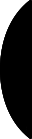
\includegraphics{symbols/llbparenthesis.png}}}}
\newcommand{\rrbparenthesis}{\vcenter{\hbox{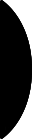
\includegraphics{symbols/rrbparenthesis.png}}}}
\newcommand{\lban}{\llparenthesis \,}
\newcommand{\rban}{\, \rrparenthesis}
\newcommand{\lbban}{\llbparenthesis \,}
\newcommand{\rbban}{\, \rrbparenthesis}
\newcommand{\banana}[1]{\lban #1 \rban}
\newcommand{\bbanana}[1]{\lbban #1 \rbban}
\newcommand{\cherry}{\rotatebox[origin=c]{270}{$\limp$}}

\newcommand{\lam}[2]{\lambda #1.\, #2}
\newcommand{\ap}[2]{#1\,#2}
\newcommand{\app}[3]{\ap{\ap{#1}{#2}}{#3}}
\newcommand{\appp}[4]{\ap{\ap{\ap{#1}{#2}}{#3}}{#4}}
\newcommand{\op}[1]{\mathtt{#1}}
\newcommand{\onto}[1]{#1 \mathalpha{:\,}}
\newcommand{\typedop}[3]{\op{#1} : #2 \rightarrowtail #3}
\newcommand{\typedopg}[3]{#1 : #2 \rightarrowtail #3}
\newcommand{\row}[2]{\{ #1 \mathrel{|} #2 \}}

\newcommand{\CC}{\mathcal{C}}
\newcommand{\FF}{\mathcal{F}}
\newcommand{\XX}{\mathcal{X}}
\newcommand{\EE}{\mathcal{E}}
\newcommand{\TT}{\mathcal{T}}
\newcommand{\PP}{\mathcal{P}}

\newcommand{\FV}{\operatorname{FV}}

\newcommand{\subst}[3]{#1[#2 \coloneqq #3]}

\newcommand{\syntclos}[1]{\mathbin{[#1]}}

\newcommand{\cibanana}{\banana{(\onto{\op{op}_i} M_i)_{i \in I},\ \onto{\eta} M_\eta}}
\newcommand{\cdbanana}{\banana{\onto{\op{op}_1} M_1,\ \dots,\ \onto{\op{op}_n} M_n,\ \onto{\eta} M_\eta}}

\newcommand{\cibbanana}{\bbanana{(\onto{\op{op}_i} M_i)_{i \in I},\ \onto{\eta} M_\eta}}

\newcommand{\TODO}[1]{\textbf{TODO}: #1}

\newcommand{\relR}{\mathbin{R}}

\newcommand{\swap}{\mathbin{\textbf{swap}}}

\newcommand{\tto}{\twoheadrightarrow}

\mathchardef\mhyphen="2D

\newcommand{\pair}[2]{\left<#1, #2\right>}
\newcommand{\inl}{\operatorname{inl}}
\newcommand{\inr}{\operatorname{inr}}

\newcommand{\true}{\textbf{T}}
\newcommand{\false}{\textbf{F}}
\newcommand{\ifte}[3]{\text{\textbf{if} $#1$ \textbf{then} $#2$ \textbf{else} $#3$}}


% Examples
\newcommand{\expr}[1]{\textsc{#1}}
\newcommand{\sume}{\expr{sum}}
\newcommand{\prode}{\expr{prod}}
\newcommand{\lite}{\expr{lit}}
\newcommand{\dive}{\expr{div}}
\newcommand{\trye}{\expr{try}}
\newcommand{\lete}{\expr{let}}
\newcommand{\vare}{\expr{var}}
\newcommand{\sumecn}[2]{\app{\sume}{#1}{#2}}
\newcommand{\prodecn}[2]{\app{\prode}{#1}{#2}}
\newcommand{\litecn}[1]{\ap{\lite}{#1}}
\newcommand{\divecn}[2]{\app{\dive}{#1}{#2}}
\newcommand{\tryecn}[2]{\app{\trye}{#1}{#2}}
\newcommand{\letecn}[3]{\appp{\lete}{\bar{#1}}{#2}{#3}}
\newcommand{\varecn}[1]{\ap{\vare}{#1}}

\newcommand{\paren}[1]{(#1)}

\newcommand{\sumec}[2]{\paren{\sumecn{#1}{#2}}}
\newcommand{\prodec}[2]{\paren{\prodecn{#1}{#2}}}
\newcommand{\litec}[1]{\paren{\litecn{#1}}}
\newcommand{\divec}[2]{\paren{\divecn{#1}{#2}}}
\newcommand{\tryec}[2]{\paren{\tryecn{#1}{#2}}}
\newcommand{\letec}[3]{\paren{\letecn{#1}{#2}{#3}}}
\newcommand{\varec}[1]{\paren{\varecn{\bar{#1}}}}


\newcommand{\NN}{\mathbb{N}}
\newcommand{\dbze}{\frac{\cdot}{0}}
\newcommand{\dbzelong}{\operatorname{DivisionByZero}}


\newcommand{\reseto}{\mathtt{reset0}}
\newcommand{\shifto}{\mathtt{shift0}}
\newcommand{\resetobanana}{\banana{\onto{\op{shift0}}{(\lam{c k}{\ap{c}{k}})}}}
\newcommand{\resetbanana}{\bbanana{\onto{\op{shift0}}{(\lam{c k}{\ap{c}{k}})}}}
\newcommand{\from}{\leftarrow}

\newcommand*{\twoheadleftrightarrow}{%
  \twoheadleftarrow
  \mathrel{\mkern-15mu}%
  \twoheadrightarrow
}

\newcommand{\ffrom}{\twoheadleftarrow}
\newcommand{\ttoffrom}{\twoheadleftrightarrow}


\newcommand{\reset}{\mathtt{reset}}
\newcommand{\shift}{\mathtt{shift}}

\newcommand{\semo}[1]{\sem{#1}_0}


\newcommand{\demph}[1]{\textbf{#1}}

\newcommand{\pipe}{\mathbin{|}}
\newcommand{\xto}[1]{\xrightarrow{#1}}

\renewcommand\theequation{\arabic{equation}}


\begin{document}

%\ThesisDraft

\dominitoc

\ThesisTitle{Les effects et les handlers \\
  dans le langage naturel \\
  ~\\
  Effects and Handlers \\ in Natural Language}
\ThesisDate{9 d\'ecembre 2016}
\ThesisAuthor{Jirka Mar\v{s}\'ik}

\ThesisUL

\ClearJury
\NewJuryCategory{President}{\textit{Pr\'esident :}}{\textit{Pr\'esidents :}}
\NewJuryCategory{Directeurs}{\textit{Directeur de th\`ese :}}{\textit{Directeurs de th\`ese :}}
\NewJuryCategory{Codirecteurs}{\textit{Co-directeur de th\`ese :}}{\textit{Co-directeurs de th\`ese :}}
\NewJuryCategory{Rapporteurs}{\textit{Rapporteur :}}{\textit{Rapporteurs :}}
\NewJuryCategory{Examinateurs}{\textit{Examinateur :}}{\textit{Examinateurs :}}
\President    = { VIGNERON Laurent & Universit\'e de Lorraine }
\Directeurs   = { DE GROOTE Philippe & Inria Nancy - Grand Est }
\Codirecteurs = { AMBLARD Maxime & Universit\'e de Lorraine }
\Rapporteurs  = { BARKER Chris & New York University \\
                  HERBELIN Hugo & Inria Paris - Rocquencourt }
\Examinateurs = { QUATRINI Myriam & Institut de Math\'ematiques de Luminy \\
                  UNGER Christina & Universit\"at Bielefeld }

\nthks

\MakeThesisTitlePage

\begin{ThesisAcknowledgments}
  I would like to thank my supervisors, whose contributions have been essential to
my work. Maxime Amblard was always eager to spend his time listening to all the
developments in my work, including numerous dead ends, and providing help and
support every step of the way. Philippe de Groote had a large impact on my work
by sharing his insight and experience with the lambda calculus, leading to some
of the most important developments in the first part of this thesis. I would
also like to thank the other members of the jury, who have all gone above and
beyond their duty and devoted their time to studying my work: Chris Barker, Hugo
Herbelin, Myriam Quatrini, Christina Unger, Laurent Vigneron.

The research presented in this manuscript was carried out within the Sémagramme
team at Inria. One of the key factors behind the quality of this work was the
friendly atmosphere at the Sémagramme team fostered by its researchers,
engineers, PhD students and interns: Clément Beysson, Sarah Blind, Vu Anh Duc,
Bruno Guillaume, Nicolas Lefebvre, Pierre Ludmann, Aleksandre Maskharashvili,
Guy Perrier, Sylvain Pogodalla, Sai Qian, Stéphane Tiv. My gratitude also
extends to all the people that made the day-to-day working conditions at Loria
very pleasant, notably the excellent staff at the restaurant, the administrative
teams handling all the paperwork (Aurélie Aubry, Céline Simon, François Thaveau)
and the many friends and colleagues that I got to play music with or chat during
lunch breaks: Mihai Andries, Benoît Chappet de Vangel, Émilie Colin, Sylvain
Contassot-Vivier, Baldwin Dumortier, Mariia Fedotenkova, Iñaki Fernández Pérez,
Francesco Giovannini, Arseniy Gorin, Meysam Hashemi, Adrien Krähenbühl, Cecilia
Lindig-Leon, Jérémy Miranda, Aybüke Özgün, Motaz Saad, Yann Salaun, Evangelia
Tsiontsiou, Jan Volec.

My decision to stay in Nancy and do a PhD with the Sémagramme team was in one
part due to an excellent introduction into the fields of formal grammar and
computational semantics that I had during my Master studies there, taught by
Maxime Amblard, Philippe de Groote, Bruno Guillaume, Guy Perrier and Sylvain
Pogodalla. The other part that made me enjoy my Master studies in Nancy so much
were my amazing classmates, talented individuals who were always eager to go to
bars on weekdays and organize study group sessions on weekends: Bruno
Andriamiarina Miharimanana, Georgy Boytchev, Caroline Ceballos, Tatiana
Ekeinhor-Komi, Nicolas Feuillet, Natalia Korchagina, Imane Nkairi, Gabin
Personeni, Wei Qiu, Camille Sauder.

During my PhD studies, I drew a lot of inspiration and motivation from my
regular visits to the European Summer School of Logic, Language and Information.
Among the many bright minds that I have had the time to discuss and spend time
with, I would like to mention Lasha Abzianidze, Eleri Aedmaa, Pepijn Kokke and
Stellan Petersson.

Before ending this section, I would also like to thank the people who have
enriched my life outside of the office. I am grateful to Marie-George Alle-Hans
for her great teaching skills during the university dancing classes. I am
forever in debt to Nelly Madigou for carefully teaching me the basics of cello
playing. I was very lucky to find and join the Orchestre Symphonique
Universitaire de Lorraine, where I got to discover the joys of orchestral
playing. I also wish to thank the many friends and flatmates who have kept me
company during my stay in Nancy: Aurélie Boizard, Orianne Cabaret, Marie Gantet,
Marine Larrière, Jordan Medic, Dorine Petit, Gautier Vacheron.

Finally, I wish to send the biggest thanks to my parents and family who have
supported me during my long studies abroad.
\end{ThesisAcknowledgments}


\begin{ThesisDedication}
  \begin{czech}
    Tuto práci věnuji \\ mým rodičům
  \end{czech}
\end{ThesisDedication}


\tableofcontents

\NoChapterHead

\NoNewPageAfterParts

\mainmatter


\chapter*{Introduction}

The motivation behind this thesis is to advance the automatic process of
translating natural language into logical representations. The interest
behind this translation procedure is two-fold: linguists use it to give a
formal semantics to natural languages and computer scientists use it to
perform automated reasoning on natural language data.

There has been considerable research into translating parts of English and
other natural languages. When looking at a sentence of English, we can
identify many of the problems inherent in the translation and point to
papers that have proposed solutions.

\begin{exe}
  \ex She might still be dating that idiot. \label{ex:intro}
\end{exe}

\begin{enumerate}
\item \label{item:first-feature} We have anaphoric expressions, such as the
  pronoun \emph{she}. We know that we can translate sentences with anaphora into
  Discourse Representation Theory~(DRT) structures~\cite{kamp1993discourse},
  Dynamic Predicate Logic~(DPL) formulas~\cite{groenendijk1991dynamic} or
  continuation-passing style $\lambda$-terms~\cite{de2006towards}.
  \item We have the modal auxiliary \emph{might} that we can translate into
    an operator of modal logic or directly to some existential
    quantification over possible worlds.
  \item We have the progressive present tense in \emph{be
      dating}. Similarly to the modal, we can translate this into an
    operator of temporal logic or directly posit the existence of some
    interval of time during which the dating takes place and assert that
    the time of utterance (possibly) lies in that interval.
  \item We have the presupposition trigger \emph{still} that tells us that
    the two subjects must have been dating in the past already. We will
    have to possess some mechanism to project this contribution outside the
    scope of any of the logical operators present.\footnote{While in the
      present, we can only infer that they \emph{might} be dating, by
      accommodating the presupposition, we can infer that sometime in the
      past, they \emph{must have been} dating.} We can adopt the strategy
    of Lebedeva~\cite{lebedeva2012expression} and raise exceptions to
    perform the projection.
  \item \label{item:last-feature} We have the expressive epithet
    \emph{idiot}. Following the theory of conventional implicatures of
    Potts~\cite{potts2005logic}, elaborated by
    Gutzmann~\cite{gutzmann2015use}, we know that we should introduce a
    second dimension into which we tuck away the speaker's negative
    attitude towards the date-ee so that it does not interfere with the
    at-issue content.
\end{enumerate}

All of the advice given above seems sound. We could follow these guidelines
to intuitively arrive at some reasonable logical representation. Now how do
we write down this joint translation process? Most of the theories
mentioned above come with their own language: their own definitions,
notation and operations.

DRT introduces its own encoding of logical formulas and states an algorithm
that builds them up incrementally from the input
sentence~\cite{kamp1993discourse}. Potts's logic of conventional
implicatures introduces two-dimensional logical formulas and defines new
modes of combination to compute with
them~\cite{potts2005logic}. Compositional treatments of intensionality or
tense tend to use the simply-typed lambda
calculus~\cite{ben2007semantics,de2013note}, as is also the case in de
Groote's treatment of anaphora~\cite{de2006towards}. In studying
presuppositions, Lebedeva uses a modified version of de Groote's calculus
which includes exceptions~\cite{lebedeva2012expression}.

It seems clear that in order to arrive at a precise notion of what it means
do all of~\ref{item:first-feature}--\ref{item:last-feature}, we will first
have to be able to express the theories behind
\ref{item:first-feature}--\ref{item:last-feature} using a common formal
language.

\section*{Enter Monads}

We will base our universal language on the $\lambda$-calculus. Thanks to
Richard Montague's hugely influential work~\cite{montague1973proper}, the
$\lambda$-calculus is already a very popular formalism in formal
compositional semantics.\footnote{Frege's compositionality principle states
  that the meanings of complex expressions should be determined by (i.e.\
  be functions of) the meanings of its constituents. If complex meanings
  are to be seen as functions of other meanings, it makes sense to use a
  calculus of functions, i.e.\ the $\lambda$-calculus.} Many phenomena are
analyzed using the $\lambda$-calculus and the rest tend to get translated
to $\lambda$-calculus as well (see, for example,
$\lambda$-DRT~\cite{kuschert1995type} or de Groote's continuation-based
approach to dynamics~\cite{de2006towards}).

However, even though we have several theories which are all formalised in
$\lambda$-calculus, it does not necessarily mean that they are compatible
or that we know how to combine them together. A theory of intensionality
might state that sentences ought to be translated to terms that have the
type $\sigma \to o$, the type of functions from possible worlds to truth
values. On the other hand, an account of expressives would argue that
sentences ought to correspond to terms of type $o \times \epsilon$, the
type of pairs of truth values (propositional content) and expressive
markers (expressive content). The two theories would be compatible at the
calculus-level but not at the term-level. A function operating with
intensional propositions would not be directly applicable to an expressive
proposition.

To continue our quest for uniformity and compatibility of semantic
operations, we will look at the terms and types used by the different
$\lambda$-theoretic treatments of semantics and try to find a common
structure underneath. We notice that all such approaches share at least the
following structure:

\begin{enumerate}
\item \label{item:type-transformation} The types of some of the denotations
  get expanded. For example, when dealing with quantifiers, the type of
  denotations of noun phrases goes from $\iota$ (single individuals) to
  $(\iota \to o) \to o$ (generalized quantifiers over individuals); in
  intensional semantics, the type of denotations of sentences goes from $o$
  (truth values) to $\sigma \to o$ (functions from possible worlds to truth
  values, i.e.\ sets of possible worlds); and with expressives, the type of
  denotations of sentences goes from $o$ to $o \times \epsilon$ (truth
  values coupled with expressive markers).
\item \label{item:monad-eta} There is a process that can lift denotations
  of the old type into denotations of the new type. In the quantifier
  example, this is the famous type raising operation. In the intensional
  example, this is the $\textbf{K}$ combinator that turns a truth value
  into a constant function that assigns that truth value to all worlds, a
  rigid intension. In the expressive example, this is the function that
  couples a proposition with a neutral/empty expressive marker.
\item Then there are other inhabitants of the expanded type that are not
  found by using the lifting function described above; those are the ones
  for which we expanded the type. Quantificational noun phrases such as
  \emph{everyone} are not the result of type raising any specific
  individual. Intensional propositions such as \emph{Hespherus is
    Phosphorus} have extensions that vary from world to world. Expressives
  such as the diminutive \emph{Wolfie} will point to some individual and
  also carry some expressive marker that conveys the speaker's attitude
  towards the referent.
\item \label{item:monad-mu} Finally, these approaches also have some
  general way of composing smaller denotations into larger ones and dealing
  with the added complexity caused by the more elaborate types. When
  applying a transitive verb to a quantificational subject and object, we
  let one (often the subject) first take scope and then we let the other
  take scope. When applying the verb to intensional arguments, we pass the
  world at which we are evaluating the sentence down to both the subject
  and the object. When applying it to expressive arguments, we apply the
  verb to the referents of both the subject and the object and on the side
  we collect the expressive content of both.
\end{enumerate}

This kind of structure is very commonly seen in functional programming and
in denotational semantics of programming languages. It is the structure of
an \emph{applicative functor}~\cite{mcbride2008applicative} (or
\emph{strong lax monoidal functor}, for the categorically-inclined). The
above examples are also instances of a more special structure called a
\emph{monad}~\cite{moggi1991notions}.

We will not go into the minutiae of the definition of a monad here but we
will give a rough sketch nonetheless. A monad is a triple
$(T, \eta, \hsbind)$ where $T$ is a function on types (the type expansion
we saw in~\ref{item:type-transformation}), $\eta$ is some way of lifting
simple values into expanded values (the lifting functions
in~\ref{item:monad-eta}) and $\hsbind$ gives us a general way of combining
values of this expanded type (similar to the examples given
in~\ref{item:monad-mu}).\footnote{This way of presenting a monad (a type
  constructor, $\eta$ and $\hsbind$) is particular to functional
  programming. Note that this presentation differs from the
  category-theoretical one which replaces $\hsbind$ with a natural
  transformation $\mu$ \cite{mac1978categories}.} The triple also has to
satisfy some algebraic properties which guarantee that composing functions
of expanded types is associative and that the lifting function serves as a
unit for this composition operator.

The examples given above are all instances of monads. The prevalence of
monads in natural language semantics has been already discovered by Shan
in~\cite{shan2002monads}. However, the challenge lies in trying to use
several monads at the same time.


\section*{Linguistic Side Effects}

Monads often appear in denotational semantics of programming languages to
account for notions of computation commonly referred to as \emph{side
  effects}~\cite{moggi1991notions}. We can base ourselves on this
correspondence and regard the monadic structure in natural language as
linguistic side effects. This analogy was pursued by
Shan~\cite{shan2005linguistic,shan2005thesis} and
Kiselyov~\cite{kiselyov2008call} and is present in recent work on monads in
natural language
semantics~\cite{giorgolo2012monads,charlow2014semantics}. However, the idea
itself stretches back before monads were even introduced to computer
science. In their 1977 paper~\cite{hobbs1977making}, Hobbs and Rosenschein
take a computational perspective on the intensional logic of
Montague~\cite{montague1973proper}: intensions correspond to programs and
extensions correspond to values. A program can read the value of global
variables that describe the state of the world.\footnote{Dependence on an
  environment of some type $\sigma$ is a side effect that can be described
  using the reader monad. This monad lifts the type $\alpha$ to the type
  $\sigma \to \alpha$. This is exactly the change of types that is
  prescribed by theories of
  intensionalization~\cite{ben2007semantics,de2013note}.} The operators
$\uparrow$ and $\downarrow$, which map between extension-denoting
expressions and intension-denoting expressions, then correspond to the
Lisp-style operators $\texttt{quote}$ and $\texttt{eval}$ respectively.

The idea of treating linguistic expressions as effectful actions or programs is
also very relevant to dynamic semantics, which treats the meanings of sentences
as instructions to update some common ground or other linguistic
context.\footnote{The use of monads to encode dynamic effects (anaphora) dates
  back to 2009 and the work of Giorgolo and
  Unger~\cite{giorgolo2009coreference,unger2012dynamic}.} Dynamic semantics and
anaphora are sometimes classified as belonging to both semantics and pragmatics.
This is also the case for other phenomena that we will treat as side effects in
our dissertation: deixis, presupposition, conventional implicature. Pragmatics
studies the way a language fits into the community of its users, i.e.\ how it is
actually used by its speakers to achieve their goals. It might then come as no
surprise that pragmatics align well with side effects in programming languages
since side effects themselves concern the ways that programs can interact with
the world of their users (e.g.\ by making things appear on screen or by
listening for the user's input).


\section*{Effects and Handlers}

By looking at the different monadic structures of natural language
semantics as side effects, we can apply theories that combine side effects
to find a formalism that can talk about all the aspects of language at the
same time. One such theoretical framework are effects and handlers. In this
framework, programs are interpreted as sequences of instructions (or more
generally as decision trees).\footnote{More precisely, we are interpreting
  programs in a free monad~\cite{swierstra2008data}.} The instructions are
symbols called \emph{operations}, which stand for the different effects,
the different ways that programs can interact with their contexts. In our
application to natural language semantics, here are some examples of
operations that will feature in our demonstrations, along with their
intended semantics:\footnote{The operations are just symbols and so have no
  inherent meaning.}

\begin{itemize}
\item $\op{introduce}$ introduces a new discourse referent to the
  context. This is the kind of operation used by noun phrases such as the
  indefinite \emph{a man}.
\item $\ap{\op{presuppose}}{P}$ presupposes the existence of an entity
  satisfying the predicate $P$. This is used by definite descriptions
  \emph{the $P$} and by proper nouns.
\item $\ap{\op{implicate}}{i}$ states that $i$ is a conventional implicature.
  This operation is used by appositive constructions such as \emph{John, who is
    my neighbor}.
\item $\op{speaker}$ asks the context for the identity of the speaker. This
  is used by the first-person pronoun to find its referent.
\end{itemize}

The process of calculating the denotation of a linguistic expression is
broken down to these operations. When expressions combine to form sentences
and discourses, these operations end up being concatenated into a large
program which will want to perform a series of interactions with its
context. This is when handlers come into play. A \emph{handler} is an
interpreter that gives a definition to the operation symbols in a
program. Handlers can be made modular~\footnote{In a similar way that
  monads can be turned into monad transformers (monad morphisms) and then
  composed~\cite{shan2002monads,wu2015transformers}.} so that the
interpreter for our vocabulary of context interactions can be defined as
the composition of several smaller handlers, each treating a different
aspect of language (dynamicity, implicatures, deixis\ldots).

When using effects and handlers, we therefore start by enumerating the set
of interactions that programs (i.e.\ linguistic expressions in our
application) can have with their contexts. Then, we can interpret
linguistic expressions as sequences of such instructions. Finally, we write
handlers which implement these instructions and produce a suitable semantic
representation. This approach thus closely follows the mantra given by
Lewis:

\begin{quote}
  In order to say what a meaning is, we may first ask what a meaning does
  and then find something that does that.

  \begin{flushright}
    General Semantics, David Lewis~\cite{lewis1970general}
  \end{flushright}
\end{quote}

We can trace the origins of effects and handlers to two strands of
work. One is Cartwright and Felleisen's work on Extensible Denotational
Language Specifications~\cite{cartwright1994extensible}, in which a
technique for building semantics is developed such that when a
(programming) language is being extended with new constructions (and new
side effects), the existing denotations remain compatible and can be
reused. The other precursor is Hyland's, Plotkin's and Power's work on
algebraic effects~\cite{hyland2006combining}, a categorical technique for
studying effectful computations, which was later extended by Plotkin and
Pretnar to include
handlers~\cite{plotkin2009handlers,pretnar2010logic,plotkin2013handling}. The
technique has gained in popularity in recent years (2012 and onward). It
finds applications both in the encoding of effects in pure functional
programming
languages~\cite{kiselyov2013extensible,kiselyov2015freer,kammar2013handlers,brady2013programming}
and in the design of programming
languages~\cite{bauer2012programming,lindley2016dobedobedo,dolan2015effective,kiselyov2016eff,hillerstrom2016compiling}. Our
thesis will explore the applicability of effects and handlers to natural
language semantics.


\section*{Plan}

The manuscript of this thesis is split into two parts. In the first, we
develop a formal calculus that extends the simply-typed lambda calculus
with a free monad for effects and handlers. We prove some key properties,
such as strong normalization, and we show how the calculus relates to other
similar notions such as continuations or monads. In the second part, we
analyze some of the aspects of linguistic meaning as side effects: deixis,
conventional implicature, quantification, anaphora and presupposition. We
then incrementally build up a fragment that features all of those features
and demonstrates some of their interactions.



\part{Calculus of Effects and Handlers}
\label{part:calculus}

We will present a calculus with special constructions for dealing with
effects and handlers, which we will then apply to the problem of natural
language semantics in the rest of the thesis. Our calculus is an extension
of the simply-typed lambda calculus (STLC). We enrich STLC with a type for
representing effectful computations alongside with operations to create and
process values of this type.

\chapter{Definitions}

We are tempted to start by first giving the formal definitions of all the
essential components of our calculus:

\begin{itemize}
\item the syntax of the terms in our calculus
\item the syntax of the types in our calculus
\item the judgments that relate types to terms
\item a reduction semantics
\end{itemize}

However, before we do so, we will briefly sketch the ideas behind the
calculus so you can start building an intuition about the meaning of the
symbols that we will be introducing below.

\section{Sketching Out the Calculus}
%% \todo{This now serves both as a sketch and a justification of the calculus,
%%   along with the history of the techniques used. This could maybe later
%%   live in its own place, somewhere in the introduction.}

We will be adding a new type constructor, $\FF$, into our
language. The type $\FF(\alpha)$ will correspond to effectful
\emph{computations} that produce values of type $\alpha$. The idea comes
from the programming language Haskell and its use of monads
\cite{moggi1991notions,wadler1992essence,jones2003haskell}. Our type
constructor $\FF$ will also stand in for a monad, one that has been
already encoded in Haskell in several ways
\cite{kiselyov2013extensible,kammar2013handlers}. The motivation behind our
calculus is thus to build a minimal language which gives us directly the
primitive operations for working with this particular monad. This way, we
end up with a language that:
\begin{itemize}
\item is smaller than Haskell (and thus more mananageable to analyse),
\item is closer to the STLC favored by semanticists,
\item and which makes more evident the features that our proposal relies on.
\end{itemize}

The transition from type $\alpha$ to a type $\FF(\alpha)$ is meant
as a generalization of a scheme often seen in semantics when novel forms of
meaning are studied (e.g., type raising \cite{montague1973proper},
dynamization \cite{lebedeva2012expression}, intensionalization
\cite{de2013note}). The distinction between the type $\alpha$ and the type
$\FF(\alpha)$ will, in different analyses, align with dichotomies
such as the following:

\begin{itemize}
\item static/dynamic meaning
\item extension/intension
\item semantics/pragmatics
\end{itemize}

The question then is, what form should our general $\FF$ type
constructor take? We want to have a construction that can combine all the
existing ones. One can do the combining at the level of monads with the use
of monad transformers, a technique pioneered by Moggi and very
well-established in the Haskell programming community
\cite{moggi1991notions}. Simon Charlow has made the case that this
technique can be exploited to great benefit in natural language semantics
as well \cite{charlow2014semantics}.

However, a competing technique has emerged in recent years and it is the
goal of this thesis to introduce it to semanticists and verify its
applicability to the study of natural language. The technique goes by many
names, ``algebraic effects and handlers'' and ``extensible effects'' being
the most commonly used ones. This is in part due to the fact that it lies
at the confluence of several research programs. This fact will allow us to
present the theory from two different perspectives so you can be equipped
with two different intuitive models.

%% Mention Lewis' ``What should meanings do instead of what should meanings
%% be.'' somewhere?

\subsubsection*{Algebraic Effects and Handlers}

Hyland, Power and Plotkin have studied the problem of deriving denotational
semantics of programming languages that combine different side effects
\cite{hyland2006combining}. In their approach, rather then modeling the
individual effects using monads and combining the monads, every effect is
expressed in terms of \emph{operators} on computations. Computations thus
become algebraic expressions with effects as operations and values as part
of the generator set.

Let us take the example of nondeterminism. In the monadic framework, this
effect is analyzed by shifting the type of denotations from $\alpha$ to the
powerset $\PP(\alpha)$. In the algebraic framework, a binary
operator $+$ is introduced and is given meaning through a set of equations.
In this case, these are the equations of a semilattice (stating the
operator's associativity, commutativity and idempotence).

When the time comes to combine two effects, their signatures are summed
together and their theories are combined through either a sum or a tensor
(a sum that adds commutativity laws for operators coming from the two
different effects).

In order to fit exception handlers into their theory, Plotkin and Pretnar
enriched the theory with a general notion of a \emph{handler}
\cite{plotkin2013handling}. A handler's purpose is to replace occurrences
of an operator within a computation by another expression. This notion was
shown to be very useful. Since using a handler on a computation is similar
to interpreting its algebraic expression in a particular algebra, in many
practical applications, the use of handlers has replaced equational
theories altogether
\cite{bauer2012programming,kammar2013handlers,brady2013programming}.

\subsubsection*{Extensible Effects}

In the early 90's, Cartwright and Felleisen were working on the following
problem. Imagine you have a simple programming language along with some
denotational semantics or some other interpretation. In your simple
language, numerical expressions might be interpreted as numbers. In that
case, the literal number 3 would denote the number 3 and the application of
the sum operator to two numerical expressions would denote the sum of their
interpretations. Now consider that you want to add mutable variables to
your language. Numerical expressions no longer denote specific numbers, but
rather functions from states of the variable store to both a number and an
updated variable store (since expressions can now both read from and write
to variables). The number 3 is thus no longer interpreted as the number 3
but as a combination of a constant function yielding the number 3 and an
identity function. The addition operator now has to take care to thread the
state of the memory through the evaluation of both of its arguments. In
short, we are forced to give new interpretations for the entire language.

Cartwright and Felleisen proposed a solution to this problem
\cite{cartwright1994extensible}. In their system, an expression can either
yield a value or produce an effect. If it produces an effect, the effect
percolates through the program all the way to the top, with the context
that the effect projected from stored as a continuation. The effect and the
continuation are then passed to an external ``authority'' that handles the
effect, often by producing some output and passing it back to the
continuation. When a new feature is added to the language, it often
suffices to add a new kind of effect and introduce a new clause into the
central ``authority''. The central authority then ends up being a
collection of small modular interpreters for the various effect
types. Denotation-wise, every expression can thus have a stable denotation
which is either a pure value or an effect request coupled with a
continuation.

Later on, this project was picked up by Oleg Kiselyov, who, following
Plotkin and Pretnar's work on handlers, proposed to break down the
``authority'' into the smaller constituent interpreters and have them be
part of the language themselves \cite{kiselyov2013extensible}.

\subsubsection*{Synthesis}

In our language, we can see values of type $\FF(\alpha)$ as
algebraic expressions built on top of some effect signature and the
generator set $\alpha$. Since an
%% \todo{Maybe introduce a more precise term
%%   which would correspond to an algebraic expression in which variables have
%%   been replaced by members of a carrier/generator set.}
{algebraic expression} is either a constant or an operator applied to some
other expressions/computations, we can also use the ``extensible effects''
perspective. Under that perspective, we can think of computations as
something which is either a pure value or an effect coupled with a
continuation (the effect corresponds to the operator and the continuation
to the indexed family of operands).

Our calculus will contain tools for injecting values of type $\alpha$ into
the type of algebraic expressions $\FF(\alpha)$, as well as tools
for constructing expressions using operators from the effect
signature. Under the ``extensible effects'' point of view, the latter can
be seen as tools for creating a computation that will raise a request to
perform an effect.

Finally, we will have a special form for defining handlers. In the
``algebraic effects and handlers'' frame of mind, these can be thought of
folds or catamorphisms that traverse the algebraic expression and transform
certain operators within. On the other hand, with ``extensible effects'',
the intuition is more similar to that of an exception handler which
intercepts requests of a certain type and decides how the computation
should continue.

\section{Terms}

Having sketched the idea behind our calculus, we will now turn our
attention to the specifics. We start by defining the syntactic
constructions used to build the terms of our language.

Without further ado, we give the syntax of the expressions of our
language. First off, let $\XX$ be a set of variables, $\Sigma$ a typed
signature and $\EE$ a set of operation symbols.

The expressions of our language are comprised of the following:
\begin{description}
  \item[abstraction] $\lam{x}{M}$, where $x$ is a variable from $\XX$ and
    $M$ is an expression
  \item[application] $\ap{M}{N}$, where $M$ and $N$ are expressions
  \item[variable] $x$, where $x$ is a variable from $\XX$
  \item[constant] $c$, where $c$ is a constant from $\Sigma$
  \item[operation] $\op{op}$, where $\op{op}$ is an operator from $\EE$
  \item[injection] $\eta$
  \item[handler] $\banana{\onto{\op{op}_1} M_1,\ \dots,\ \onto{\op{op}_n} M_n,\ 
                          \onto{\eta} M_\eta}$
    where $\op{op}_i$ are operators from $\EE$ and $M_i$ and $M_\eta$ are
    expressions
  \item[extraction] $\cherry$
  \item[exchange] $\CC$
\end{description}

The first four constructions --- abstraction, application, variables and
constants --- come directly from STLC with constants.

The next four deal with the algebraic expressions used to encode
computations. Let us sketch the behaviors of these four kinds of
expressions under the two readings outlined above.

\subsection*{Algebraic Expressions -- The Denotational View}

The $\eta$ function serves to inject values from the generator set into the
set of algebraic expressions. It is a constructor for the trivial atomic
algebraic expression consisting of just a single constant.

Next, for every symbol $\op{op}$ in $\EE$, we have a corresponding function
$\op{op}$ in our calculus. The function $\op{op}$ is a constructor for
algebraic expressions whose topmost operation is $\op{op}$. The $\op{op}$
constructor takes as argument a function that provides its operands, which
are further algebraic expressions.

The banana brackets $\banana{\onto{\op{op}_1}
  M_1,\ \dots,\ \onto{\op{op}_n} M_n,\ \onto{\eta} M_\eta}$ contain algebras:
interpretations of operators and constants. These components are combined
into a catamorphism that can interpret algebraic expressions (hence the use
of banana brackets \cite{meijer1991functional})\footnote{Since the banana
  brackets can contain an arbitrary number of operator clauses, we use the
  syntax of named parameters/records commonly used in popular programming
  languages such as Ruby, Python or JavaScript.}.

The extraction function $\cherry$, pronounced ``cherry'', takes an atomic
algebraic expression (the kind produced by $\eta$) and projects out the
element of the generator set.

\subsection*{Effectful Computations -- The Operational View}

We will now explain these constructions from the computational point of
view.

The $\eta$ function ``returns'' a given value. The result of applying it to
a value $x$ is a computation that immediately terminates and produces the
value $x$.

The symbols from $\EE$ become something like system calls. A computation
can interrupt its execution and throw an exception with a request to
perform a system-level operation. For every symbol $\op{op}$ in $\EE$,
there is a constructor $\op{op}$ that produces a computation which issues a
request to perform the operation $\op{op}$. This constructor takes as an
argument a continuation which yields the computation that should be pursued
after the system-level operation $\op{op}$ has been performed.

The banana brackets $\banana{\onto{\op{op}_1}
  M_1,\ \dots,\ \onto{\op{op}_n} M_n,\ \onto{\eta} M_\eta}$ describe
handlers: they contain clauses for different kinds of interrupts (operation
requests) and for successful computations (clause $\eta$). They behave very
much like handlers in languages with resumable exceptions such as Common
Lisp or Dylan.

Finally, the cherry function $\cherry$ can take a computation that is
guaranteed to be free of side effects and run it to capture its result.

\vspace{2em}

The 9th construction in our calculus is the $\CC$ operator. $\CC$ serves as
a link between the function type discussed by STLC (constructions 1--4) and
the computation type introduced in our calculus (constructions 5--8). $\CC$
is a (partial) function that takes a computation that produces a function
and returns a function that yields computations. In a way, $\CC$ makes
abstracting over a variable and performing an operation commute
together\footnote{This is \emph{very} reminiscent of the idea behind Paul
  Blain Levy's call-by-push-value calculus \cite{levy1999call}, which
  treats abstracting over a variable as an effectful operation of popping a
  value from a stack. Using call-by-push-value should prove to be a
  rewarding way to refine our approach.}.

We will see the utility of $\CC$ later on. The idea came to us from a paper
by Philippe de Groote \cite{degroote2015conservativity} which tried to
solve a similar problem. The name comes from the $\mathbf{C}$ combinator,
which reorders the order of abstractions in a $\lambda$-term. $\mathbf{C}$
can be seen as a special case of our $\CC$ when the type of computations
producing values $\alpha$ is $\gamma \to \alpha$ for some $\gamma$.


\section{Types and Typing Rules}

We now give a syntax for the types of our calculus alongside with a typing
relation. In the grammar below, $\nu$ ranges over atomic types from set
$\TT$.

The types of our language consist of:
\begin{description}
\item[function] $\alpha \to \beta$, where $\alpha$ and $\beta$ are types
\item[atom] $\nu$, where $\nu$ is an atomic type from $\TT$
\item[computation] $\FF_E(\alpha)$, where $\alpha$ is a type and $E$ is an
  effect signature (defined next)
\end{description}

The only novelty here is the $\FF_E(\alpha)$
computation\footnote{Throughout this manuscript, we will be using the term
  \emph{computation} to mean values of type $\FF_E(\alpha)$. Programs
  written in our calculus are simply called terms and their normal forms
  are called values. To break it down, in our calculus, terms evaluate to
  values, some of which can be computations (those of an $\FF$ type).}
type. This type will be inhabited by effectful computations that have
permission to perform the effects described in $E$ and yield values of type
$\alpha$. The representation will be that of an algebraic expression with
operators taken from the signature $E$ and constants (elements of the
generator set) taken to be in type $\alpha$.

In giving the typing rules, we will rely on the standard notion of a
\emph{context}. For us, specifically, a context is a partial mapping from
the variables in $\XX$ to the types defined above.  We commonly write
$\Gamma, x : \alpha$ for a context that assigns to $x$ the type $\alpha$
and to other variables $y$ the type $\Gamma(y)$. We also write $x : \alpha
\in \Gamma$ to say that the context maps $x$ to $\alpha$. Note, however,
that for $\Delta = \Gamma, x : \alpha, x : \beta$, $x : \beta \in \Delta$
while $x : \alpha \notin \Delta$.

\emph{Effect signatures} are very much like contexts. They are partial
mappings from the set of operation symbols $\EE$ to pairs of types. We will
write the elements of effect signatures the following way:
$\typedop{op}{\alpha}{\beta} \in E$ means that $E$ maps $\op{op}$ to the
pair of types $\alpha$ and $\beta$\footnote{The two types $\alpha$ and
  $\beta$ are to be seen as the operation's \emph{input} and \emph{output}
  types, respectively.}. When dealing with effect signatures, we will often
make use of the disjoint union operator $\uplus$. The term $E_1 \uplus E_2$
serves as a constraint demanding that the domains of $E_1$ and $E_2$ be
disjoint and at the same time it denotes the effect signature that is the
union of $E_1$ and $E_2$.

The last kind of dictionary used by the type system is a standard
\emph{higher-order signature} for the constants (a map from names of
constants to types). For those, we adopt the same conventions.

In our typing judgments, contexts will appear to the left of the turnstile
and they will hold information about the \emph{statically} (lexically)
bound variables, as in STLC.\@ Effect signatures will appear as indices of
computation types and they will hold information about the operations that
are \emph{dynamically} bound by handlers. Finally, there will be a single
higher-order signature that will globally characterize all the available
constants.

The typing judgments are presented in Figure~\ref{fig:types}. Metavariables
$M$, $N$\ldots\ stand for expressions, $\alpha$, $\beta$,
$\gamma$\ldots\ stand for types, $\Gamma$, $\Delta$\ldots\ stand for
contexts, $\op{op}$, $\op{op}_i$ stand for operation symbols and $E$,
$E'$\ldots\ stand for effect signatures. $\Sigma$ refers to the
higher-order signature giving types to constants.

\newcommand{\handlerrule}{
 \begin{prooftree}
  \AxiomC{$E = \{\typedopg{\op{op}_i}{\alpha_i}{\beta_i}\}_{i \in I} \uplus E_f$}
  \noLine
  \def\extraVskip{0pt}
  \UnaryInfC{$E' = E'' \uplus E_f$}
  \noLine
  \UnaryInfC{$[\Gamma \vdash M_i : \alpha_i \to (\beta_i \to
    \FF_{E'}(\delta)) \to \FF_{E'}(\delta)]_{i \in I}$}
  \noLine
  \UnaryInfC{$\Gamma \vdash M_\eta : \gamma \to \FF_{E'}(\delta)$}
  \def\extraVskip{2pt}
  \RightLabel{[$\banana{}$]}
  \UnaryInfC{$\Gamma \vdash \banana{(\onto{\op{op}_i}{M_i})_{i \in I},\ \onto{\eta}{M_\eta}} : \FF_{E}(\gamma) \to \FF_{E'}(\delta)$}
 \end{prooftree}}

\begin{figure}
  \def\labelSpacing{4pt}

  \begin{subfigure}{.5\textwidth}
   \begin{prooftree}
    \AxiomC{$\Gamma, x : \alpha \vdash M : \beta$}
    \RightLabel{[abs]}
    \UnaryInfC{$\Gamma \vdash \lam{x}{M} : \alpha \to \beta$}
   \end{prooftree}
  \end{subfigure}
  \begin{subfigure}{.5\textwidth}
   \begin{prooftree}
    \AxiomC{$\Gamma \vdash M : \alpha \to \beta$}
    \AxiomC{$\Gamma \vdash N : \alpha$}
    \RightLabel{[app]}
    \BinaryInfC{$\Gamma \vdash M N : \beta$}
   \end{prooftree}
  \end{subfigure}

  \vspace{2mm}
 
  \begin{subfigure}{.5\textwidth}
   \begin{prooftree}
    \AxiomC{$x : \alpha \in \Gamma$}
    \RightLabel{[var]}
    \UnaryInfC{$\Gamma \vdash x : \alpha$}
   \end{prooftree}
  \end{subfigure}
  \begin{subfigure}{.5\textwidth}
   \begin{prooftree}
    \AxiomC{$c : \alpha \in \Sigma$}
    \RightLabel{[const]}
    \UnaryInfC{$\Gamma \vdash c : \alpha$}
   \end{prooftree}
  \end{subfigure}

  \vspace{6mm}

  \begin{subfigure}{.5\textwidth}
   \begin{prooftree}
    \AxiomC{$\Gamma \vdash \eta : \alpha \to \FF_E(\alpha)$
    \hskip 4pt [$\eta$]}
   \end{prooftree}
  \end{subfigure}
  \begin{subfigure}{.5\textwidth}
   \begin{prooftree}
    \AxiomC{$\Gamma \vdash \cherry : \FF_\emptyset(\alpha) \to \alpha$
    \hskip 4pt [$\cherry$]}
   \end{prooftree}
  \end{subfigure}

  \vspace{3mm}

  \hspace{-1.5cm}
  \begin{subfigure}{.5\textwidth}
   \begin{prooftree}
    \AxiomC{$\typedop{op}{\alpha}{\beta} \in E$}
    \RightLabel{[op]}
    \UnaryInfC{$\Gamma \vdash \op{op} : \alpha \to (\beta \to \FF_E(\gamma)) \to \FF_E(\gamma)$}
   \end{prooftree}
  \end{subfigure}
  \hspace{1cm}
  \begin{subfigure}{.5\textwidth}
   \handlerrule
  \end{subfigure}

  \vspace{6mm}

  \begin{subfigure}{\textwidth}
   \begin{prooftree}
    \AxiomC{$\Gamma \vdash \CC : (\alpha \to \FF_E(\beta)) \to
      \FF_E(\alpha \to \beta)$
    \hskip 4pt [$\CC$]}
   \end{prooftree}
  \end{subfigure}

  \caption{\label{fig:types}Typing rules for our calculus.}
\end{figure}


The typing rules mirror the syntax of expressions. Again, the first four
rules come from STLC.\@ The next four deal with introducing pure
computations, enriching them with effectful operations, handling those
operations away and finally eliminating pure computations. The $\CC$ rule
lets us start to see what we meant by saying that the $\CC$ operator lets
the function type and the computation type commute.

Let us ponder the types of the new constructions so as to get a grip on the
interface that the calculus provides us for dealing with computation
values.

\subsection*{[$\eta$]}

First off, we have the $\eta$ operator. It takes a value of type $\alpha$
and injects it into the type $\FF_E(\alpha)$. The meta-variable $E$ is
free, meaning $\eta$ can take values of type $\alpha$ to type
$\FF_E(\alpha)$ for any $E$. The algebraic intuition would say that elements
of the generator set are valid algebraic expressions independent of the
choice of signature. Computationally, returning a value is always an
option, independently of the available permissions.

\subsection*{[op]}

More complicated computations can be built up by extending existing
computations using the \textbf{operation} construction. Let us have an
effect signature $E$, such that $\typedop{op}{\alpha}{\beta} \in E$. To use
$\op{op}$, we first apply it to a value of the input type $\alpha$ and to a
continuation. The continuation is a function of type $\beta \to
\FF_E(\gamma)$ that accepts a value of the output type $\beta$ (the result
of performing the operation) and chooses in return a computation that
should be pursued next. The return type of our new computation will thus be
the return type $\gamma$ of the computation provided by the
continuation. The continuation's computation and the new extended
computation will also share the same effect signature $E$. This means that
all uses of the operation $\op{op}$ within the created computation have the
same input and output types\footnote{In general, the same operation symbol
  can be used in different computations whose types are indexed by
  different effect signatures.}.

Notice also how the [op] rule is similar to the [var] rule in that it lets
use a symbol with a certain type given that it exists in some kind of
signature/context. The crucial difference is that contexts are components
of judgments whereas effect signatures are components of types. The meaning
of a variable is determined by inspecting the expression in which it occurs
and finding the $\lambda$ that binds it (this is known as \emph{lexical} or
\emph{static binding}). On the other hand, the meaning of an operation in a
computation is determined by evaluating the term in which the computation
appears until the computation becomes the argument of a handler. This
handler will then give meaning to the operation symbol by effectively
substituting it with a suitable interpretation (this kind of \emph{late}
binding is known as \emph{dynamic binding}).

We have now seen how to construct pure computations using $\eta$ and extend
them by adding operations. However, before we go on and start talking about
handlers, we would like to give the algebraic intuition behind [op], as the
algebraic point of view makes explaining the handler rule [$\banana{}$]
easier.

We can see the effect signature as an algebraic signature. Whenever we have
$\typedop{op}{\alpha}{\beta} \in E$, we have an $\alpha$-indexed family of
operators of arity $\beta$. Let's unpack this statement.

\begin{itemize}
\item First, there is the matter of having an indexed family of
  operators. A common example of these is the case of scalar multiplication
  in the algebra of a vector space. A \emph{single-sorted algebraic
    signature} is a set of operation symbols, each of which is given an
  arity (a natural number). For vector addition, the arity is 2, since
  vector addition acts on two vectors (two elements of the
  domain). Scalar multiplication acts on one scalar and one
  vector. However, neither arity 1 nor arity 2 adequately express this. We
  can get around the limitations of a single-sorted signature by
  introducing for every scalar $k$ an operation of arity 1 that corresponds
  to multiplying the vector by $k$. Scalar multiplication is therefore not
  a single operator but a scalar-indexed family of operators.

  The very same strategy is applied here as well. A single operation symbol
  doesn't need to map to a single operator but can instead map to (possibly
  infinitely) many operators indexed by values of some type $\alpha$. For
  example, writing messages to the program's output
  ($\typedop{print}{string}{1}$) can be seen as a string-indexed family of
  unary operators on computations. For every string $s$, we get an operator
  that maps computations $c$ to computations that first print $s$ and then
  continue as $c$.

\item Next, we were speaking about operators of arity $\beta$. The use of a
  type in place of a numerical arity is due to a certain generalization. In
  set theory, natural numbers become sets that have the same cardinality as
  the number they represent ($\left\vert N \right\vert = N$). We can
  therefore conservatively generalize the idea of arity to a set by saying
  that an operator of arity $X$ takes one operand per each element of the
  set $X$. It's a short step from there to using types as arities, wherein
  an operator of arity $\beta$ takes one operand per possible value of type
  $\beta$.

  This will come in very handy in our system. We want our operator
  $\op{op}$ to have as many operands as there are possible values in the
  output type $\beta$. Therefore, we simply say that the operator has arity
  $\beta$.

  How do we write down the application of an operator of arity $\beta$ to
  its operands? We can no longer just list out all the operands, since
  types in our calculus may have an unbounded number of inhabitants. We
  will organize operands in \emph{operand clusters}\footnote{Our use of the
  word \emph{cluster} is synonymous with the mathematical term
  \emph{family}. We will be using the term \emph{cluster} for families of
  computations passed to operations and handlers.}, arity-indexed families
  of operands. We will write them down as functions, using
  $\lambda$-abstraction, from the arity type $\beta$ to some operand type,
  e.g., $\FF_E(\gamma)$.
\end{itemize}

Now we can understand what it means to say that
$\typedop{op}{\alpha}{\beta} \in E$ gives rise to an $\alpha$-indexed
family of operators of arity $\beta$. We apply to $\op{op}$ an index of
type $\alpha$ to get an operator and then we apply that operator to an
operand cluster of type $\beta \to \FF_E(\gamma)$ to get a new expression
of type $\FF_E(\gamma)$.

We suggest visualizing these algebraic expressions as trees (see Section~2
of \cite{lindley2014algebraic} for the original idea). Trees of type
$\FF_E(\alpha)$ consist of leafs containing values of type $\alpha$ and
internal nodes labelled with operations and their parameters. Every
internal node is labelled with some $\typedop{op}{\alpha}{\beta} \in E$ and
with a parameter of type $\alpha$ and it has a cluster of children indexed
by $\beta$.

\subsection*{[$\banana{}$]}

Now we are ready to explain the handler rule. Let us have some computation
$N : \FF_E(\gamma)$ (which we can now think of as an algebraic
expression or a tree). By applying the handler
$\banana{(\onto{\op{op}_i}{M_i})_{i \in I},\ \onto{\eta}{M_\eta}}$ to $N$,
we get a new computation $N' : \FF_{E'}(\delta)$. The typing rule
for $\banana{}$ is repeated in Figure~\ref{fig:handler-rule}.

\begin{figure}
  \handlerrule
  \caption{\label{fig:handler-rule} The typing rule for the handler
    construction.}
\end{figure}

To illustrate the constraints on the types of the components, $M_i$ and
$M_\eta$, of a handler, we will examine its semantics. The handler
processes the tree $N$ by recursive induction. Depending on the shape of
the tree, one of the following will happen:

\begin{itemize}
\item If $N$ is a leaf, then the value stored in the leaf is of type
  $\gamma$. This is where the $M_\eta$ function comes in. It must take a
  value of type $\gamma$ and produce a new tree of type $\FF_{E'}(\delta)$,
  hence the fourth hypothesis of the $\banana{}$ rule.

\item If $N$ is an internal node labelled with the operation symbol
  $\op{op}_i$ for some $i \in I$ and some parameter, then that parameter
  must be of type $\alpha_i$. Furthermore, this node will have a
  $\beta_i$-indexed cluster of children. We know this since $N$ is of type
  $\FF_E(\gamma)$ and the first hypothesis tells us that
  $\typedopg{\op{op}_i}{\alpha_i}{\beta_i} \in E$.

  We will recursively apply our handler to the cluster of children,
  changing their type from $\FF_E(\gamma)$ to $\FF_{E'}(\delta)$. We now
  need something which takes the parameter in the node, type $\alpha_i$,
  and the family of the processed subtrees, type $\beta_i \to
  \FF_{E'}(\delta)$, which is exactly the function $M_i$ in the third
  hypothesis of the $\banana{}$ rule.

\item If $N$ is an internal node labelled with some operation symbol
  $\op{op}$ such that $\typedop{op}{\alpha}{\beta} \in E_f$ for some
  $\alpha$ and $\beta$, then we will ignore the node and process only its
  children. This means that the resulting tree will contain the operation
  $\op{op}$ and any other symbols defined in $E_f$\footnote{The $f$ in
    $E_f$ stands for \emph{forwarded effects}, since it refers to effects
    that the handler will not interpret but instead forward to some other
    interpreter.}. In order for such a tree to be of the desired type
  $\FF_{E'}(\delta)$, $E_f$ must be a subset of $E'$, which is what the
  second hypothesis of the $\banana{}$ rule guarantees.
\end{itemize}

We have covered the whole $\banana{}$ rule, except for the presence of the
effect signature $E''$. It serves two roles.

\begin{itemize}
\item First of all, it acts as a ``free'' variable over effect
  signatures. This means that we can give any effect signature $E'$ to the
  type $\FF_{E'}(\delta)$ of the resulting computation $N'$ as long as $E'$
  contains $E_f$ ($E''$ represents the relative complement of $E_f$ in
  $E'$). This is in analogy to the free effect variable $E$ in the [$\eta$]
  and [op] rules. This freedom of effect variables is a way of implementing
  the idea that a computation of type $\FF_{E_1}(\alpha)$ can be used
  anywhere that a computation of type $\FF_{E_2}(\alpha)$ given that $E_1
  \subseteq E_2$\footnote{This relation is an instance of subtyping and a
    more robust treatment will be outlined in Section~\ref{sec:subtyping}.}.

\item In the previous paragraph, why did we put the word ``free'' in
  quotation marks?  Because the effect variable $E''$ is not actually
  free. It is the complement of $E_f$ in $E'$ and $E'$ is constrained by
  the types of $M_i$ and $M_\eta$ in the third and fourth hypotheses,
  respectively. The handler's clauses might themselves introduce new
  effects, which will in turn translate into constraints on $E'$ and
  $E''$. This happens when a handler interprets an operation by making an
  appeal to some other operation (e.g.\ a handler can interpret
  computations using n-ary choice into computation using binary choice).

  As the simplest example, we can take a handler that replaces one
  operation symbol with another,
  $\banana{\onto{\op{old}} \op{new},\ \onto{\eta} \eta}$. The type scheme
  corresponding to the term is $\FF_{\{\typedop{old}{\alpha}{\beta}\}
    \uplus E_f}(\gamma) \to \FF_{\{\typedop{new}{\alpha}{\beta}\} \uplus
    E^3 \uplus E_f}(\gamma)$. In this scheme, $\alpha$, $\beta$ and
  $\gamma$ are free meta-variables ranging over types and $E_f$ and $E^3$
  are free over effect signatures. The $E''$ of the $\banana{}$ rule
  corresponds to $\{\typedop{new}{\alpha}{\beta}\} \uplus E^3$. The handler
  has eliminated the $\op{old}$ effect but it has also introduced the
  $\op{new}$ effect.
\end{itemize}

This concludes our exploration of the $\banana{}$ rule. We have explained
it in terms of algebraic expressions and trees, using the denotational
intution. We will develop the operational intuition, which talks about
handlers in terms of computations and continuations, in
Section~\ref{sec:reductions}, where we will give the semantics of our
language using reduction rules.

\subsection*{[cherry]}

Next up is the cherry operator, $\cherry$. Its type is
$\FF_\emptyset(\alpha) \to \alpha$ and it serves as a kind of dual to the
$\eta$ opertator, an elimination for the $\FF$ type.

The type $\FF_\emptyset(\alpha)$ demands that the effect signature be
empty. In such a case, the tree has no internal nodes and is composed of
just a leaf containing a value of the type $\alpha$. The $\cherry$ operator
serves to extract that value.

Another way to look at it is to say that a computation of type
$\FF_\emptyset(\alpha)$ cannot perform any ``unsafe'' operations and it is
therefore always safe to execute it and get the resulting value of type
$\alpha$.

\subsection*{[$\CC$]}

Finally, we take a look at the $\CC$ operator. The type of the operator is
$(\alpha \to \FF_E(\beta)) \to \FF_E(\alpha \to \beta)$. Its input is an
$\alpha$-indexed family of computations and its output is a computation of
$\alpha$-indexed families. The operator applies only in the case when all
the computations in the family share the same \emph{internal structure}. By
sharing the same \emph{internal structure}, we mean that the trees can only
differ in their leaves. What the $\CC$ operator then does is to push the
$\lambda$-binder down this common internal structure into the leaves (see
Figure~\ref{fig:c-illustration} for an example). This way, we can
evaluate/handle the common operations without commiting to a specific value
of type $\alpha$.

\begin{figure}
  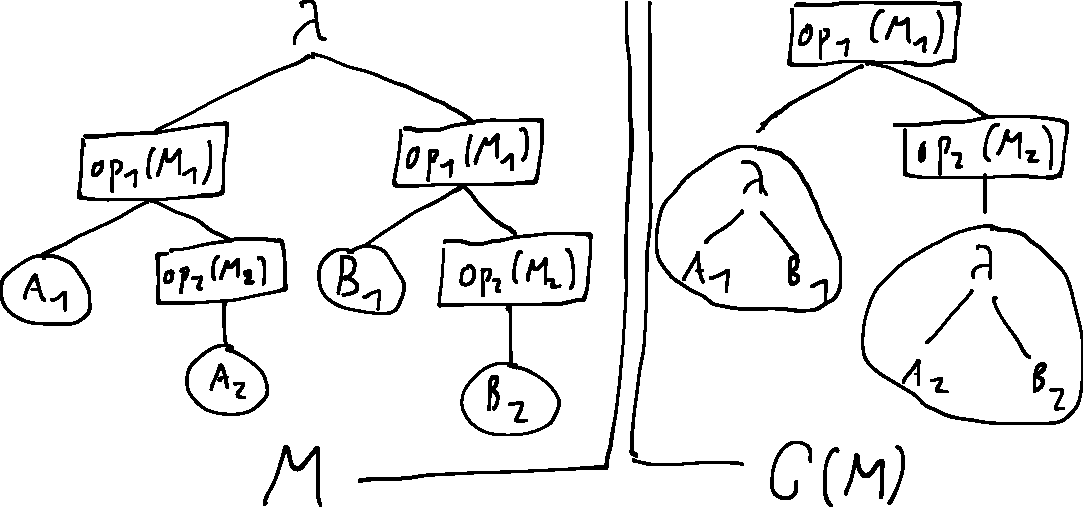
\includegraphics[width=\textwidth]{doodles/c-illustration}
  \caption{\label{fig:c-illustration} Example of applying the $\CC$
    operator to a term. Functions/families are drawn as trees. In this
    example, the $\lambda$ binds a variable of a binary type, the output of
    $\op{op}_1$ is binary and the output of $\op{op}_2$ is unary. TODO:
    This doodle is a placeholder for a cleaner picture generated by a
    program (or at least until I learn to draw).}
\end{figure}

We can also explain the action of $\CC$ in operational terms. As in
call-by-push-value~\cite{levy1999call}, we can think of abstraction over
$\alpha$ as some effectful operation that tries to pop a value $x : \alpha$
off a stack. The input of $\CC$ can then be seen as a continuation waiting
for this $x$ and wanting to perform some further operations. $\CC$ assumes
that the continuation performs operations independently of
$x$\footnote{Violating this assumption will yield terms which get stuck
  during evaluation (we will see the partial reduction rules in
  Section~\ref{sec:reductions}). Sam Lindley presented a refined type
  system for a similar calculus to track the use of variables
  \cite{lindley2014algebraic}. A similar refinement should be possible in
  our case as well but it would obscure the already dense type notation.}
and it can thus postpone popping $x$ off the stack until after the
operations dictated by the continuation have been evaluated. $\CC$ is thus
a kind of commutativity law for operations and abstraction (the popping of
a value off the operand stack): as long as one does not depend on the
other, it does not matter whether we first perform an operation and then
abstract over an argument or whether we do so the other way
around\footnote{The other direction, typed $\FF_E(\alpha \to \beta) \to
  (\alpha \to \FF_E(\beta))$, is already possible without introducing a
  special operator since $\FF_E$ is a functor (as we will show later).}.


\section{Reduction Rules}
\label{sec:reductions}

We will now finally give a semantics to our calculus. The semantics will be
given in the form of a reduction relation on terms. Even though the point
of the calculus is to talk about effects, the reduction semantics will have
no notion of order of evaluation or evaluation context; any subexpression
that is reducible can be reduced in any context.

Before we dive into the reduction rules proper we will first have to handle
some formal paperwork.

\begin{definition}
  Let $\sim$ be a binary relation on the terms of our calculus. We define
  the relation $\syntclos{\sim}$, called the \emph{syntactic closure} of
  $\sim$, as the smallest relation that contains $\sim$ and satisfies the
  following conditions:

  \begin{itemize}
  \item if $M \sim M'$, then $\lam{x}{M} \syntclos{\sim} \lam{x}{N}$
  \item if $M \sim M'$, then $\ap{M}{N} \syntclos{\sim} \ap{M'}{N}$
  \item if $N \sim N'$, then $\ap{M}{N} \syntclos{\sim} \ap{M}{N'}$
  \item if $M_i \sim M_i'$, then $\banana{\onto{\op{op}_1}
    M_1,\ \dots,\ \onto{\op{op}_i} M_i,\ \dots,\ \onto{\op{op}_n}
    M_n,\ \onto{\eta}{M_\eta}} \syntclos{\sim} \banana{\onto{\op{op}_1}
    M_1,\ \dots,\ \onto{\op{op}_i} M_i',\ \dots,\ \onto{\op{op}_n}
    M_n,\ \onto{\eta} M_\eta}$
  \item if $M_\eta \sim M_\eta'$, then
    $\banana{(\onto{\op{op}_i}{M_i})_{i \in I},\ \onto{\eta}{M_\eta}}
    \syntclos{\sim} \banana{(\onto{\op{op}_i}{M_i})_{i \in I},\ \onto{\eta}{M_\eta'}}$
  \end{itemize}
\end{definition}

We will now present a set of type-preserving rules that we will use to
evaluate/simplify expressions in our language.

\vspace{3mm}

\begin{tabular}{lr}
  $(\lambda x.\ M)\ N \rightarrow$ & [$\beta$] \\
  $M[x \coloneqq N]$ & \\
  \\
  $[\mathcal{H}\ (OP_i\ M_i)\ldots\ (\eta\ M_\eta)]\ (\eta\ N) \rightarrow$ & [$\mathcal{H}$-$\eta$] \\
  $M_\eta\ N$ & \\
  \\
  $[\mathcal{H}\ (OP_i\ M_i)\ldots\ (\eta\ M_\eta)]\ (OP_i\ N_a\ N_k) \rightarrow$ & [$\mathcal{H}$-$OP$] \\
  $M_i\ N_a\ (\lambda x.\ [\mathcal{H}\ (OP_i\ M_i)\ldots\ (\eta\ M_\eta)]\ (N_k\ x))$ & where $x$ is fresh \\
  \\
  $[\mathcal{H}\ (OP_i\ M_i)\ldots\ (\eta\ M_\eta)]\ (OP\ N_a\ N_k) \rightarrow$ & [$\mathcal{H}$-$OP^*$] \\
  $OP\ N_a\ (\lambda x.\ [\mathcal{H}\ (OP_i\ M_i)\ldots\ (\eta\ M_\eta)]\ (N_k\ x))$ & where $x$ is fresh \\
  & and $OP \notin \{OP_i\}_i$ \\
  \\
  $\mathcal{C}\ (\lambda x.\ \eta\ M) \rightarrow$ & [$\mathcal{C}$-$\eta$] \\
  $\eta\ (\lambda x.\ M)$ & \\
  \\
  $\mathcal{C}\ (\lambda x.\ OP\ M_a\ M_k) \rightarrow$ & [$\mathcal{C}$-$OP$] \\
  $OP\ M_a\ (\lambda y.\ \mathcal{C}\ (\lambda x.\ M_k\ y))$ & where $y$ is fresh \\
  & and $x \notin FV(M_a)$
\end{tabular}

\vspace{3mm}

Besides the standard $\beta$-reduction rule, we have rules that define the
behavior of the handlers formed using $\mathcal{H}$ and of the
$\mathcal{C}$ operator.


\section{Sums and Products}


\section{Common Combinators}

Here we will introduce a collection of generally useful syntactic shortcuts
and combinators for our calculus.

\begin{align*}
  \_ \circ \_ &: (\beta \to \gamma) \to (\alpha \to \beta) \to (\alpha \to \gamma) \\
  f \circ g &= \lambda x.\ f\ (g\ x) \\
  \_^* &: (\alpha \to \mathcal{F}(\beta)) \to (\mathcal{F}(\alpha) \to \mathcal{F}(\beta)) \\
  f^* &= [\mathcal{H}\ (\eta\ f)] \\
  \mathcal{F} &: (\alpha \to \beta) \to (\mathcal{F}(\alpha) \to \mathcal{F}(\beta)) \\
  \mathcal{F} &= \lambda f.\ (\eta \circ f)^* \\
  \_ \hsbind \_ &: \mathcal{F}(\alpha) \to (\alpha \to \mathcal{F}(\beta)) \to \mathcal{F}(\beta) \\
  M \hsbind N &= N^*\ M \\
  \\
  [\mathcal{H}\ (OP_i\ M_i)\ldots] &= [\mathcal{H}\ (OP_i\ M_i)\ldots\ (\eta\ \eta)]
\end{align*}

We will also make use of combinators for function application where one or
more of the arguments are computations.

\begin{align*}
  \_ \apl \_ &: \mathcal{F}(\alpha \to \beta) \to \alpha \to \mathcal{F}(\beta) \\
  F \apl x &= F \hsbind (\lambda x.\ \eta\ (f\ x)) \\
  \_ \apr \_ &: (\alpha \to \beta) \to \mathcal{F}(\alpha) \to \mathcal{F}(\beta) \\
  f \apr X &= X \hsbind (\lambda x.\ \eta\ (f\ x))
\end{align*}


\chapter{Examples}
\label{chap:examples}

We have given a formal definition of our calculus but we have not shown how
to use it to model side effects and what are the benefits. In this chapter,
we will present an example problem and as we explore it deeper, we will see
emerge some of the properties behind our calculus.

\minitoc

\section{Introducing Our Running Example}

We will try to build a calculator. Given some arithmetic expression, we
would like to reduce it to a simple number. 

$$
\app{\sume}{(\ap{\lite}{1})}{(\app{\prode}{(\ap{\lite}{2})}{(\ap{\lite}{4})})}
\quad \to \quad 9
$$

In the above, expressions are formed using the constructors $\sume$,
$\prode$ and $\lite$ which stand for sums, products and literals,
respectively. Expressions in our calculator have the type $exp$, the types
of the constructors (formation rules) are given below\footnote{The type
  $\NN$ is the type of natural numbers. Since our examples will deal with
  numbers, we will treat naturals as terms of our calculus that have the
  type $\NN$. Their syntax and equational theory are both standard so we
  will not repeat it here.}:

\begin{align*}
  \sume &: exp \to exp \to exp \\
  \prode &: exp \to exp \to exp \\
  \lite &: \NN \to exp
\end{align*}

The exercise is similar to our enterprise of formal semantics. We have a
language (fragment) with a formal grammar and we try to find a systematic
way of identifying sentences of this language with their senses or
references. Our methodology will also be the same of formal semantics: a
composition of meanings that mirrors the syntactic structure.

Before we go on, a quick technical remark about the $exp$ type and its
encoding. A common approach is to model $exp$ as an inductive
algebraic data type\footnote{This would be something called an
  \emph{initial encoding} of a language.} and then have our calculator be a
function from $exp$ to $\NN$ or some other domain of
interpretation. Our calculus does not directly provide inductive types but
the $\FF$ type constructor is built on top of them and since it is
parameterizable by an effect signature, it can be used to implement a
variety of inductive types. In this particular scenario, we could use
$\FF_{\{\typedop{sum}{1}{2},\typedop{prod}{1}{2}\}}(\NN)$ as
$exp$. The notion of a closed handler ($\bbanana{}$, see
$\ref{ssec:operations-and-handlers}$) would then give use the induction
principle over these arithmetic expression, i.e.\ a way to compositionally
compute some value from the arithmetic expression.

We will not be using the encoding described above. The point of this
chapter is to make the reader familiar with the notion of using the
$\FF$-types to model computations. We will therefore restrict their use to
computations.

We can avoid introducing any kind of type for encoding arithmetic
expressions. The reduction step from an arithmetic expression to a simple
number can be realized by adding equations that ``define'' the functions
$\sume$, $\prode$, $\lite$ and the type $exp$. We thus take $exp$ to be the
name of the type of our desired interpretations and we take $\sume$,
$\prode$ and $\lite$ to be some functions that compute directly with these
interpretations\footnote{This is known as a \emph{final encoding} of a
  language.}. The task of the semanticist is to fix some specific
interpretation for the abstract type $exp$ and figuring out the definitions
of the abstract functions $\sume$, $\prode$ and $\lite$\footnote{As we will
  see in Chapter~\ref{chap:intro-fs} when we introduce them, this is
  exactly the idea behind abstract categorial grammars
  \cite{de2001towards}.}. Within our tiny fragment, this is quite easy to
do:

\begin{align*}
  exp &= \NN \\
  \sume &= \lam{x y}{x + y} \\
  \prode &= \lam{x y}{x \times y} \\
  \lite &= \lam{x}{x}
\end{align*}

Applying these equations to the term
$\app{\sume}{(\ap{\lite}{1})}{(\app{\prode}{(\ap{\lite}{2})}{(\ap{\lite}{4})})}$
and then reducing according to the reduction rules of our calculus
(alongside with rules/equations to perform arithmetic operations), we get
the result, $9$.


\section{Adding Errors}

We will now try expanding our fragment by adding integer division.

\begin{align*}
  \dive &: exp \to exp \to exp
\end{align*}

We could be tempted to treat this the same way and simply give this
semantics to $\dive$:

\begin{align*}
  \dive &= \lam{x y}{x / y}
\end{align*}

However, this assumes that we have a division operator that defines the
division $x/y$ for all naturals $x$ and $y$. This is not the case when $y =
0$. Defining $x/0$ to be some specific natural $d$ is not satisfactory
since then we cannot distinguish between the cases when $x/y$ is $d$ and
when $x/y$ is not defined. Fortunately, this is what sum types are very
useful for. We will have the type of $x/y$ be $\NN + 1$, $x/0$ will reduce
to $(\ap{\inr}{\star})$ and $x/y$ for $y \neq 0$ will reduce to
$(\ap{\inl}{q})$ where $q$ is the greatest natural such that $q y \le
x$.

\subsection{Raising the Type of $exp$}
\label{ssec:raising-the-type-of-exp}

Now the cases when $x/y$ is and is not defined are clearly
delimited\footnote{Realizing that $x/y$ is not defined for $y = 0$ and then
  changing the type and behavior of the underlying division operator is
  very much like semanticists taking into account that expressions such as
  \emph{the King of France} need not have a reference and then changing the
  underlying model by switching from functions to
  relations.}. Nevertheless, we just made ourselves a new problem. The
result of a division is something of type $\NN + 1$ and so in our
interpretation, $exp$ will correspond to $\NN + 1$. This is in line with
our intuition that arithmetic expressions which contain division can
sometimes be undefined. However, the implications of having $exp = \NN + 1$
begin to sting when we consider the cases of $\sume$ and
$\prode$\footnote{As a convention, we use $\_$ as a variable name for
  variables whose values are never used.}.

\begin{align*}
  exp &= \NN + 1 \\
  \dive &= \lam{X Y}{\case{X}{x}{\case{Y}{y}{x / y}{\_}{\ap{\inr}{\star}}}{\_}{\ap{\inr}{\star}}} \\ 
  \sume &= \lam{X Y}{\case{X}{x}{\case{Y}{y}{\ap{\inl}{(x + y)}}{\_}{\ap{\inr}{\star}}}{\_}{\ap{\inr}{\star}}} \\ 
  \prode &= \lam{X Y}{\case{X}{x}{\case{Y}{y}{\ap{\inl}{(x \times y)}}{\_}{\ap{\inr}{\star}}}{\_}{\ap{\inr}{\star}}} \\ 
  \lite &= \lam{x}{\ap{\inl}{x}}
\end{align*}


the calculation only if both of the operands successfully yield a
natural\footnote{If you are unfamiliar with the notation used in the terms
  above, consult Section~\ref{sec:sums-and-products} where we introduced
  sums and products into our calculus.}. In $\sume$, $\prode$ and $\lite$,
we also have to wrap the result in $\inl$ in order to go from $\NN$ to $\NN
+ 1$\footnote{We $\eta$ reduce the definition of $\lite$ for
  convenience.}. In $\dive$, we do not wrap the result using $\inl$ since
division already produces a value of type $\NN + 1$. All this seems a heavy
price to pay just to include division.

\subsection{Refactoring with Monads}
\label{ssec:refactoring-with-monads}

We can make this solution look a little bit better. We can introduce a
function on types and a pair of combinators that will allow us to be a
little less repetitive.

\begin{align*}
  T_\bot(\alpha) &= \alpha + 1 \\
  \eta_\bot &: \alpha \to T_\bot(\alpha) \\
  \eta_\bot &= \inl \\
  (\hsbind_\bot) &: T_\bot(\alpha) \to (\alpha \to T_\bot(\beta)) \to T_\bot(\beta) \\
  (\hsbind_\bot) &= \lam{X k}{\case{X}{x}{\ap{k}{x}}{\_}{\ap{\inr}{\star}}}
\end{align*}

With these in our hands, we can now straighten out our interpretation.

\begin{align*}
  exp &= T_\bot(\NN) \\
  \dive &= \lam{X Y}{X \hsbind_\bot (\lam{x}{Y \hsbind_\bot (\lam{y}{x / y})})} \\
  \sume &= \lam{X Y}{X \hsbind_\bot (\lam{x}{Y \hsbind_\bot (\lam{y}{\ap{\eta_\bot}{(x + y)}})})} \\
  \prode &= \lam{X Y}{X \hsbind_\bot (\lam{x}{Y \hsbind_\bot (\lam{y}{\ap{\eta_\bot}{(x \times y)}})})} \\
  \lite &= \lam{x}{\ap{\eta_\bot}{x}}
\end{align*}

This pattern that we uncovered in the type $\NN + 1$ and the terms defining
$\dive$, $\sume$, $\prode$ and $\lite$ is not incidental. The triple
$\left<T_\bot, \eta_\bot, \hsbind_\bot \right>$ forms a monad\footnote{This
  way of presenting a monad (a type constructor, $\eta$ and $\hsbind$) is
  particular to functional programming. Note that this presentation differs
  from the category-theoretical one which replaces $\hsbind$ with a natural
  transformation $\mu$ \cite{mac1978categories}.}. This formulation in
terms of monadic operations will allow us to transition more easily into
our proposed solution since, as we will show in~\ref{ssec:monad},
$\left< \FF_E, \eta, \hsbind \right>$ also forms a monad.

\subsection{Interpreting Expressions as Computations}

We will now explore an alternative solution which takes advantage of the
$\FF$-types in our calculus. We will interpret expressions as computations
of naturals, $exp = \FF_E(\NN)$. Computations will have the ability to fail
by using the operation $\typedop{fail}{1}{0}$. The input type $1$ means
that there is only one way to fail (i.e.\ $\op{fail}$ does not distinguish
failure states) and the output type $0$ means that there is no continuation
(formally there is a dummy continuation that accepts the impossible type
$0$). There is a natural way to generalize this approach by using
$\typedop{error}{\chi}{0}$ instead. Computations can now terminate by
throwing exceptions of type $\chi$, allowing us to distinguish failure
states. To identify the division-by-zero failure state, we will introduce
$\dbzelong : \chi$. A computation that uses the $\op{error}$ operation to
throw a division-by-zero exception would look like the following:

\begin{align*}
  \dbze &: \FF_{\{\typedop{error}{\chi}{0}\}}(\alpha) \\
  \dbze &= \app{\op{error}}{\dbzelong}{(\lam{o}{\absurd{o}})}
\end{align*}

The continuation uses the [empty] rule to turn the $o$ of type $0$ into
something of type $\FF_E(\alpha)$.

\begin{align*}
  exp &= \FF_{\{\typedop{error}{\chi}{0}\}}(\NN) \\
  \dive &= \lam{X Y}{X \hsbind (\lam{x}{Y \hsbind (\lam{y}{\case{(x / y)}{z}{\ap{\eta}{z}}{\_}{\dbze}})})} \\
  \sume &= \lam{X Y}{X \hsbind (\lam{x}{Y \hsbind (\lam{y}{\ap{\eta}{(x + y)}})})} \\
  \prode &= \lam{X Y}{X \hsbind (\lam{x}{Y \hsbind (\lam{y}{\ap{\eta}{(x \times y)}})})} \\
  \lite &= \lam{x}{\etaE{x}}
\end{align*}

Let us compare this with the last set of definitions:

\begin{itemize}
\item We replaced the $\left< T_\bot, \eta_\bot, \hsbind_\bot \right>$ monad
  with the $\left< \FF_{\{\typedop{error}{\chi}{0}\}}, \eta, \hsbind \right>$ monad.
\item Since the type of $x / y$ is not the same as the type of our
  interpretations, we need to translate from the type $\NN + 1$ to the type
  $\FF_{\{\typedop{error}{\chi}{0}\}}(\NN)$ by case analysis.
\end{itemize}

The advantage to using the $\FF_E$ monad instead of the $T_\bot$ monad is
that the $\FF_E$ can be extended to handle other kinds of effects besides
exceptions whereas the $T_\bot$ monad need would need to be replaced by a
different one. We will see an example of this later
in~\ref{sec:enriching-the-context-with-variables}. For now, we still have
something more to explore regarding errors.

\subsection{Handling Errors}

We can now use division in our small calculator language. However, division
can make the evaluation of an expression fail and yield no useful
result. We could thus ask for a way to speculatively evaluate a
subexpression and if it fails, recover by providing some default value and
carry on evaluating the rest of the expression.

We add a new construction into our language:

$$
\trye : exp \to exp \to exp
$$

Its intended meaning is to return the value of its second
argument. However, if the second argument fails to evaluate, the value of
the first argument should be used instead.

$$
\app{\trye}{(\ap{\lite}{42})}{(\app{\dive}{(\ap{\lite}{1})}{(\ap{\lite}{0})})}
\quad \to \quad \ap{\eta}{42}
$$

Our task now is to give a formal semantics to $\trye$.

$$
\trye = \lam{X Y}{\ap{\banana{\onto{\op{error}}{(\lam{e k}{X})}}}{Y}}
$$

Instead of passing $Y$ through the $\hsbind$ operator, which basically says
to do whatever $Y$ would do (i.e.\ fail whenever $Y$ fails), we apply a
handler to $Y$\footnote{Feeding it into $\hsbind$ or applying a handler to
  it are the two most common ways we will be using computations.}. This
handler is very simple, it replaces any failed computation with the
computation $X$ (the backup computation that should yield the default
value). It behaves like the exception handlers of common programming
languages, whenever the computation $Y$ would throw an $\op{error}$, we
handle it by running computation $X$ instead.

\subsection{Examples of Errors}

We now have enough interesting material to play around with a little bit
and see if (and why) it really works as it should. We will take an
expression large enough to contain all the features which we added and we
will evaluate it piece by piece.

$$
\app{\sume}{\litec{5}}{\tryec{\litec{0}}{\prodec{\litec{3}}{\divec{\litec{2}}{\litec{0}}}}}
$$

Let's start with $\app{\dive}{\litec{2}}{\litec{0}}$.

\NoChapterPrefix
\begin{align}
  \app{\dive}{\litec{2}}{\litec{0}}
  &= \app{\dive}{(\ap{\eta}{2})}
                {(\ap{\eta}{0})} \\
  &= \app{(\lam{X Y}{X \hsbind (\lam{x}{Y \hsbind (\lam{y}
          {\case{(x / y)}{z}{\ap{\eta}{z}}{\_}{\dbze}})})})}
                {(\ap{\eta}{2})} {(\ap{\eta}{0})} \\
  &\to_{\beta,\beta} (\ap{\eta}{2}) \hsbind (\lam{x}{(\ap{\eta}{0}) \hsbind (\lam{y}
          {\case{(x / y)}{z}{\ap{\eta}{z}}{\_}{\dbze}})}) \\
  &= \ap{(\lam{x}{(\ap{\eta}{0}) \hsbind (\lam{y}
          {\case{(x / y)}{z}{\ap{\eta}{z}}{\_}{\dbze}})})^*}{(\ap{\eta}{2})} \\
  &= \ap{\banana{\onto{\eta}{(\lam{x}{(\ap{\eta}{0}) \hsbind (\lam{y}
          {\case{(x / y)}{z}{\ap{\eta}{z}}{\_}{\dbze}})})}}}{(\ap{\eta}{2})} \\
  &\to_{\banana{\eta}} \ap{(\lam{x}{(\ap{\eta}{0}) \hsbind (\lam{y}
          {\case{(x / y)}{z}{\ap{\eta}{z}}{\_}{\dbze}})})}{2} \\
  &\to_{\beta} (\ap{\eta}{0}) \hsbind (\lam{y}
          {\case{(2 / y)}{z}{\ap{\eta}{z}}{\_}{\dbze}}) \\
  &\to_{\ldots} \ap{(\lam{y}{\case{(2 / y)}{z}{\ap{\eta}{z}}{\_}{\dbze}})}{0} \\
  &\to_{\beta} \case{(2 / 0)}{z}{\ap{\eta}{z}}{\_}{\dbze} \\
  &\to_{/} \case{(\ap{\inr}{\star})}{z}{\ap{\eta}{z}}{\_}{\dbze} \\
  &\to_{\beta.+_2} \dbze
\end{align}
\setcounter{equation}{0}
\ChapterPrefix

The reductions state which rule was used to perform the step. The equality
on line 2 is due to our interpretation of $\dive$. Those on lines 4 and 5
come from the definitions of $\hsbind$ and $^*$
in~\ref{ssec:composing-functions}. The step on line 8 is just a repeat of
the steps on lines 4 to 6. This sequence of steps will be quite common and
we will from now on refer to it as the reduction rule
$\eta.\hsbind$\footnote{This rule will be formally introduced
  in~\ref{ssec:bind}. It says that whenever we have
  $(\ap{\eta}{x}) \hsbind k$, we can reduce this to $\ap{k}{x}$.}

The result of this first elaboration was not surprising: dividing 2 by 0
throws a $\dbzelong$ exception. We will now try to see what happens when
this faulty expression appears within another expression.

\NoChapterPrefix
\begin{align}
  \app{\prode}{\litec{3}}{\dbze}
  &= \app{\prode}{(\ap{\eta}{3})}{\dbze} \\
  &= \app{(\lam{X Y}{X \hsbind (\lam{x}{Y \hsbind (\lam{y}{\ap{\eta}
          {(x \times y)}})})})}
      {(\ap{\eta}{3})}{\dbze} \\
  &\to_{\beta,\beta} (\ap{\eta}{3}) \hsbind (\lam{x}{\dbze \hsbind (\lam{y}{\ap{\eta}
          {(x \times y)}})}) \\
  &\to_{\eta.\hsbind} \ap{(\lam{x}{\dbze \hsbind (\lam{y}{\ap{\eta}
          {(x \times y)}})})}{3} \\
  &\to_{\beta} \dbze \hsbind (\lam{y}{\ap{\eta} {(3 \times y)}}) \\
  &= (\app{\op{error}}{\dbzelong}{(\lam{o}{\absurd{o}})}) \hsbind (\lam{y}{\ap{\eta} {(3 \times y)}}) \\
  &= \ap{(\lam{y}{\ap{\eta} {(3 \times y)}})^*}{(\app{\op{error}}{\dbzelong}{(\lam{o}{\absurd{o}})})} \\
  &= \ap{\banana{\onto{\eta}{(\lam{y}{\ap{\eta} {(3 \times y)}})}}}{(\app{\op{error}}{\dbzelong}{(\lam{o}{\absurd{o}})})} \\
  &\to_{\banana{\op{op}'}} \app{\op{error}}{\dbzelong}{(\lam{z}{\ap{\banana{\onto{\eta}{(\lam{y}{\ap{\eta} {(3 \times y)}})}}}{(\absurd{z})}})} \\
  &\simeq \dbze
\end{align}
\setcounter{equation}{0}
\ChapterPrefix

Line 2 is due to our interpretation of $\prode$. Line 4 is due to the
$\eta.\hsbind$ rule that we have demonstrated in the last example. Lines 6,
7 and 8 expand the definitions of $\dbze$, $\hsbind$ and $^*$. On line 10,
we equate the term with $\dbze$. The terms differ in the continuation but
since the continuation can never be called\footnote{Technical aside: To be
  precise, we should define $\dbze$ to be a class of terms of the shape
  $\app{\op{error}}{\dbzelong}{M}$ for any term $M$. The only operations we
  will ever perform on $\dbze$ in these examples will be congruent with the
  equivalence relation of our calculus refined by adding equalities between
  terms of the shape $\app{\op{error}}{\dbzelong}{M}$. Therefore, so long
  as we end up removing the $\dbze$ terms from our result, we can treat
  them as equivalent during our calculations.}, we can consider them equal.

We have seen the $\dbzelong$ exception propagate. Now let's see what
happens when it hits a $\trye$ construction.

\NoChapterPrefix
\begin{align}
  \app{\trye}{\litec{0}}{\dbze}
  &= \app{\trye}{(\ap{\eta}{0})}{\dbze} \\
  &= \app{(\lam{X Y}{\ap{\banana{\onto{\op{error}}{(\lam{e k}{X})}}}{Y}})}{(\ap{\eta}{0})}{\dbze} \\
  &\to_{\beta,\beta} \ap{\banana{\onto{\op{error}}{(\lam{e k}{\ap{\eta}{0}})}}}{\dbze} \\
  &= \ap{\banana{\onto{\op{error}}{(\lam{e k}{\ap{\eta}{0}})}}}{(\app{\op{error}}{\dbzelong}{(\lam{o}{\absurd{o}})})} \\
  &\to_{\banana{\op{op}}} \app{(\lam{e k}{\ap{\eta}{0}})}{\dbzelong}{(\lam{z}{\ap{\banana{\onto{\op{error}}{(\lam{e k}{\ap{\eta}{0}})}}}{(\absurd{z})}})} \\
  &\to_{\beta,\beta} \ap{\eta}{0}
\end{align}
\setcounter{equation}{0}
\ChapterPrefix

Line 2 is our interpretation of $\trye$. Line 4 is the definition of
$\dbze$.

We see that since the embedded expression failed to evaluate (its sense was
$\dbze$), we have evaluated the literal 0 instead. We now have an actual
number again and we can try feeding it into another operation.

\NoChapterPrefix
\begin{align}
  \app{\sume}{\litec{5}}{(\ap{\eta}{0})}
  &= \app{\sume}{(\ap{\eta}{5})}{(\ap{\eta}{0})} \\
  &= \app{(\lam{X Y}{X \hsbind (\lam{x}{Y \hsbind (\lam{y}{\ap{\eta}{(x + y)}})})})}{(\ap{\eta}{5})}{(\ap{\eta}{0})} \\
  &\to_{\beta,\beta} (\ap{\eta}{5}) \hsbind (\lam{x}{(\ap{\eta}{0}) \hsbind (\lam{y}{\ap{\eta}{(x + y)}})}) \\
  &\to_{\eta.\hsbind} \ap{(\lam{x}{(\ap{\eta}{0}) \hsbind (\lam{y}{\ap{\eta}{(x + y)}})})}{5} \\
  &\to_{\beta} (\ap{\eta}{0}) \hsbind (\lam{y}{\ap{\eta}{(5 + y)}}) \\
  &\to_{\eta.\hsbind} \ap{(\lam{y}{\ap{\eta}{(5 + y)}})}{0} \\
  &\to_{\beta} \ap{\eta}{(5 + 0)} \\
  &\to_+ \ap{\eta}{5}
\end{align}
\setcounter{equation}{0}
\ChapterPrefix

Line 2 is our interpretation of $\sume$. The others are reductions of the
kind we have seen before.

Finally, we see the simplest case when an operator just reaches into the
results of both operands using $\to_{\eta.\hsbind}$ and carries out its
operation. This also concludes our evaluation of the expression we have
presented at the beginning of this subsection. We can therefore now
conclude that:

$$
\app{\sume}{\litec{5}}{\tryec{\litec{0}}{\prodec{\litec{3}}{\divec{\litec{2}}{\litec{0}}}}}
\quad \to \quad \ap{\eta}{5}
$$


\section{Enriching the Context with Variables}
\label{sec:enriching-the-context-with-variables}

Sometimes, when writing down arithmetic expressions, it becomes useful to
introduce variables for intermediate expressions and then build up the
final result using those. Let's try and add such a facility to our
calculator.

\begin{align*}
  \lete &: var \to exp \to exp \to exp \\
  \vare &: var \to exp \\
  \bar{x}, \bar{y}, \bar{z},\ldots &: var
\end{align*}

$\lete$ binds a variable to the result of the first expression; this
variable stays available during the evaluation of the second
expression. $\vare$ then lets us use the variable in place of an
expression. We also introduce terms for the different variables that can be
used in our calculator. They look the same as the variables in our calculus
but with a bar on top.

Here is a term that uses the new constructions:

\begin{align*}
& \letecn{x}{\sumec{\litec{2}}{\litec{3}}}
 {\\ & \hspace{9mm} \letec{y}{\prodec{\varec{x}}{\varec{x}}}
 {\\ & \hspace{19mm} \prodec{\varec{y}}{\litec{2}}}} \quad \to \quad \ap{\eta}{50}
\end{align*}

In order to give a semantics to $\lete$ and $\vare$, we will augment the
set of operations in the computations we use to interpret the
expressions. We want computations to be able to ask for the values of
variables and so we will introduce $\typedop{get}{var}{\NN}$. In our new
interpretation, we will have $exp =
\FF_{\{\typedop{error}{\chi}{0},\typedop{get}{var}{\NN}\}}(\NN)$. Though it
might seem that we are changing our domain of interpretation and will thus
need to redo our existing interpretations, it is actually not the case. The
type that we associated with $exp$ before could have been more precisely
written as $\FF_{\{\typedop{error}{\chi}{0}\} \uplus E}(\NN)$, where $E$ is
a free variable ranging over effect signatures. What we are doing is simply
specifying $E = \{\typedop{get}{var}{\NN}\} \uplus E'$, where $E'$ is again
free.

\begin{align*}
  \lete &= \lam{v X Y}{X \hsbind
    (\lam{x}{\ap{\banana{\onto{\op{get}}{(\lam{u k}{\ifte{u = v}{(\ap{k}{x})}{(\app{\op{get}}{u}{k})}})}}}{Y}})} \\
  \vare &= \op{get}!
\end{align*}

In the implementation above, we also rely on the presence of an equality
predicate on the $var$ type:

 $$
  (=) : var \to var \to 2
 $$

And that is all we need. We can put these two combinators side-by-side with
the existing ones like $\dive$ and $\trye$ and we will have a semantics for
a calculator with exceptions and variables.

\subsection{Example with Variables}

To get some practice with the calculus, we will evaluate a simple
expression with multiple variables, step by step.

$$
\letecn{x}{\litec{1}}{\letec{y}{\litec{2}}{\sumec{\varec{x}}{\varec{y}}}}
$$

Let us start off with the innermost expression, the sum of $\bar{x}$ and
$\bar{y}$.

\NoChapterPrefix
\begin{align}
  \sumecn{\varec{x}}{\varec{y}}
  & = \sumecn{(\ap{\op{get}!}{\bar{x}})}
    {(\ap{\op{get}!}{\bar{y}})} \\
  & = \app{(\lam{X Y}{X \hsbind (\lam{x}{Y \hsbind (\lam{y}{\ap{\eta}{(x + y)}})})})}
    {(\ap{\op{get}!}{\bar{x}})}
    {(\ap{\op{get}!}{\bar{y}})} \\
  & \to_{\beta,\beta} (\ap{\op{get}!}{\bar{x}}) \hsbind (\lam{x}{
    (\ap{\op{get}!}{\bar{y}}) \hsbind (\lam{y}{
    \ap{\eta}{(x + y)}})}) \\
  & = (\ap{(\lam{p}{\app{\op{get}}{p}{(\lam{x}{\etaE{x}})}})}{\bar{x}}) \hsbind (\lam{x}{
    (\ap{\op{get}!}{\bar{y}}) \hsbind (\lam{y}{
    \ap{\eta}{(x + y)}})}) \\
  & \to_{\beta} (\app{\op{get}}{\bar{x}}{(\lam{x}{\etaE{x}})}) \hsbind (\lam{x}{
    (\ap{\op{get}!}{\bar{y}}) \hsbind (\lam{y}{
    \ap{\eta}{(x + y)}})}) \\
  & = \ap{\banana{\onto{\eta}{(\lam{x}{(\ap{\op{get}!}{\bar{y}}) \hsbind (\lam{y}{
    \ap{\eta}{(x + y)}})})}}}{(\app{\op{get}}{\bar{x}}{(\lam{x}{\etaE{x}})})} \\
  & \to_{\banana{\op{op}'}} \app{\op{get}}{\bar{x}}
    {(\lam{x}{\ap{\banana{\onto{\eta}{(\lam{x}{(\ap{\op{get}!}{\bar{y}})
    \hsbind (\lam{y}{\ap{\eta}{(x + y)}})})}}}{(\ap{\eta}{x})}})} \\
  & \to_{\banana{\eta}} \app{\op{get}}{\bar{x}}
    {(\lam{x}{\ap{(\lam{x}{(\ap{\op{get}!}{\bar{y}})
    \hsbind (\lam{y}{\ap{\eta}{(x + y)}})})}{x}})} \\
  & \to_{\beta} \app{\op{get}}{\bar{x}}
    {(\lam{x}{(\ap{\op{get}!}{\bar{y}})
    \hsbind (\lam{y}{\ap{\eta}{(x + y)}})})} \\
  & \to_{\ldots} \app{\op{get}}{\bar{x}}
    {(\lam{x}{\app{\op{get}}{\bar{y}}{(\lam{y}{\ap{\eta}{(x + y)}})}})}
\end{align}
\setcounter{equation}{0}
\ChapterPrefix

The first three lines are the usual. First, we expand the definitions of
the operands (the $\vare$ operator). Then we do the same for the operation
$\sume$ and we $\beta$ reduce.

On line 4, we substitute $\op{get}!$ with the definition of the exclamation
mark that we provided in~\ref{ssec:operations-and-handlers}. Similarly, on
line 6, we expand the definition of $\hsbind$\footnote{$\hsbind$ is defined
  in terms of $^*$, which is itself defined in terms of $\banana{}$. Here,
  we expand both in one go, i.e.\ $(x \hsbind f) =
  (\ap{\banana{\onto{\eta}{f}}}{x})$}.

If you compare line 3 and line 9 (the second to last line), you will
notice that they are practically identical. The $(\ap{\op{get}!}{\bar{x}})
\hsbind k$ on line 3 has been replaced with
$\app{\op{get}}{\bar{x}}{k}$. This is encapsulated in a rule named
$\op{op}!.\hsbind$ that will be introduced in Chapter~\ref{chap:properties}
and which lets us replace $(\ap{\op{op}!}{x}) \hsbind k$ with
$\app{\op{op}}{x}{k}$.

On the last line, we simply repeat the last 6 steps (which we now packaged
into the $\op{op}!.\hsbind$ rule) for $\ap{\op{get}!}{\bar{y}}$.

We have our result, a computation that asks for the values of the variables
$\bar{x}$ and $\bar{y}$ to compute their sum. Now we will compute the value
of $\app{\lete}{\bar{y}}{\litec{2}}$.

\NoChapterPrefix
\begin{align}
  \app{\lete}{\bar{y}}{\litec{2}}
&= \app{\lete}{\bar{y}}{(\ap{\eta}{2})} \\
&= \appp{(\lam{v X Y}{X \hsbind (\lam{x}{\ap{\banana{\onto{\op{get}} {(\lam{u k}{\ifte{u = v}{(\ap{k}{x})} {(\app{\op{get}}{u}{k})}})}}}{Y}})})} {\bar{y}}{(\ap{\eta}{2})} \\
&\to_{\beta,\beta} \lam{Y}{(\ap{\eta}{2}) \hsbind (\lam{x}{\ap{\banana{\onto{\op{get}}{(\lam{u k}{\ifte{u = \bar{y}}{(\ap{k}{x})}{(\app{\op{get}}{u}{k})}})}}}{Y}})} \\
&\to_{\eta.\hsbind} \lam{Y}{\ap{(\lam{x}{\ap{\banana{\onto{\op{get}}{(\lam{u k}{\ifte{u = \bar{y}}{(\ap{k}{x})}{(\app{\op{get}}{u}{k})}})}}}{Y}})}{2}} \\
&\to_{\beta} \lam{Y}{\ap{\banana{\onto{\op{get}}{(\lam{u k}{\ifte{u = \bar{y}}{(\ap{k}{2})}{(\app{\op{get}}{u}{k})}})}}}{Y}} \\
&\to_{\eta} \banana{\onto{\op{get}}{(\lam{u k}{\ifte{u = \bar{y}}{(\ap{k}{2})}{(\app{\op{get}}{u}{k})}})}}
\end{align}
\setcounter{equation}{0}
\ChapterPrefix

Lines 1 and 2 are our interpretations of $\lite$ and $\lete$ and the rest
are applications of rules we have seen before. We find out that the
semantic action of $\app{\lete}{\bar{y}}{\litec{2}}$ is a handler. This
handler is only interested in $\op{get}$ operations that act on the
variable $\bar{y}$. It interprets such operations by returning the value
$2$, otherwise it leaves them untouched.

We will now apply this handler to the meaning of
$\sumecn{\varec{x}}{\varec{y}}$ to get the meaning of
$\letecn{y}{\litec{2}}{\sumec{\varec{x}}{\varec{y}}}$.

\NoChapterPrefix
\begin{align}
  & \letecn{y}{\litec{2}}{\sumec{\varec{x}}{\varec{y}}} \\
= & \letecn{y}{\litec{2}}
       {(\app{\op{get}}{\bar{x}} {(\lam{x}{
         \app{\op{get}}{\bar{y}}{(\lam{y}{\ap{\eta}{(x + y)}})}})})} \\
= & \ap{\banana{\onto{\op{get}}{(\lam{u k}{\ifte{u = \bar{y}}
        {(\ap{k}{2})}{(\app{\op{get}}{u}{k})}})}}}
       {(\app{\op{get}}{\bar{x}} {(\lam{x}{
         \app{\op{get}}{\bar{y}}{(\lam{y}{\ap{\eta}{(x + y)}})}})})} \\
\to_{\banana{\op{op}}} &
  \app{(\lam{u k}{\ifte{u = \bar{y}}{(\ap{k}{2})}{(\app{\op{get}}{u}{k})}})}
      {\bar{x}}
      {(\lam{x}{\appp{\lete}{\bar{y}}{\litec{2}}
                   {(\app{\op{get}}{\bar{y}}{(\lam{y}{\ap{\eta}{(x + y)}})})}})} \\
\to_{\beta} &
  \ap{(\lam{k}{\ifte{\bar{x} = \bar{y}}{(\ap{k}{2})}{(\app{\op{get}}{\bar{x}}{k})}})}
     {(\lam{x}{\appp{\lete}{\bar{y}}{\litec{2}}
                  {(\app{\op{get}}{\bar{y}}{(\lam{y}{\ap{\eta}{(x + y)}})})}})} \\
\to_= &
  \ap{(\lam{k}{\ifte{\false}{(\ap{k}{2})}{(\app{\op{get}}{\bar{x}}{k})}})}
     {(\lam{x}{\appp{\lete}{\bar{y}}{\litec{2}}
                  {(\app{\op{get}}{\bar{y}}{(\lam{y}{\ap{\eta}{(x + y)}})})}})} \\
\to_{\textbf{if}.\false} &
  \ap{(\lam{k}{(\app{\op{get}}{\bar{x}}{k})})}
     {(\lam{x}{\appp{\lete}{\bar{y}}{\litec{2}}
                  {(\app{\op{get}}{\bar{y}}{(\lam{y}{\ap{\eta}{(x + y)}})})}})} \\
\to_{\beta} &
  \app{\op{get}}{\bar{x}}
     {(\lam{x}{\appp{\lete}{\bar{y}}{\litec{2}}
                  {(\app{\op{get}}{\bar{y}}{(\lam{y}{\ap{\eta}{(x + y)}})})}})} \\
= &
  \app{\op{get}}{\bar{x}}
     {(\lam{x}{\ap{\banana{\onto{\op{get}}{(\lam{u k}{\ifte{u = \bar{y}}
                                          {(\ap{k}{2})}{(\app{\op{get}}{u}{k})}})}}}
                  {(\app{\op{get}}{\bar{y}}{(\lam{y}{\ap{\eta}{(x + y)}})})}})} \\
\to_{\banana{\op{op}}} &
  \app{\op{get}}{\bar{x}}
     {(\lam{x}{(\app{(\lam{u k}{\ifte{u = \bar{y}}
                                     {(\ap{k}{2})}{(\app{\op{get}}{u}{k})}})}
                    {\bar{y}}{(\lam{y}{\appp{\lete}{\bar{y}}{\litec{2}}{(\ap{\eta}{(x + y)})}})})})} \\
\to_{\beta} &
  \app{\op{get}}{\bar{x}}
     {(\lam{x}{(\ap{(\lam{k}{\ifte{\bar{y} = \bar{y}}
                                     {(\ap{k}{2})}{(\app{\op{get}}{\bar{y}}{k})}})}
                    {(\lam{y}{\appp{\lete}{\bar{y}}{\litec{2}}{(\ap{\eta}{(x + y)})}})})})} \\
\to_= &
  \app{\op{get}}{\bar{x}}
     {(\lam{x}{(\ap{(\lam{k}{\ifte{\true}
                                     {(\ap{k}{2})}{(\app{\op{get}}{\bar{y}}{k})}})}
                    {(\lam{y}{\appp{\lete}{\bar{y}}{\litec{2}}{(\ap{\eta}{(x + y)})}})})})} \\
\to_{\textbf{if}.\true} &
  \app{\op{get}}{\bar{x}}
     {(\lam{x}{(\ap{(\lam{k}{\ap{k}{2}})}
                   {(\lam{y}{\appp{\lete}{\bar{y}}{\litec{2}}{(\ap{\eta}{(x + y)})}})})})} \\
\to_{\beta} &
  \app{\op{get}}{\bar{x}}
     {(\lam{x}{\ap{(\lam{y}{\appp{\lete}{\bar{y}}{\litec{2}}{(\ap{\eta}{(x + y)})}})}
                  {2}})} \\
\to_{\beta} &
  \app{\op{get}}{\bar{x}}
     {(\lam{x}{\appp{\lete}{\bar{y}}{\litec{2}}{(\ap{\eta}{(x + 2)})}})} \\
= &
  \app{\op{get}}{\bar{x}}
     {(\lam{x}{\ap{\banana{\onto{\op{get}}{(\lam{u k}{\ifte{u = \bar{y}}
                                          {(\ap{k}{2})}{(\app{\op{get}}{u}{k})}})}}}
                  {(\ap{\eta}{(x + 2)})}})} \\
\to_{\banana{\eta}} & \app{\op{get}}{\bar{x}} {(\lam{x}{\ap{\eta}{(x + 2)}})}
\end{align}
\setcounter{equation}{0}
\ChapterPrefix

This one is a bit more complicated and so we will go through it line by
line:


\begin{description}

  \item[Line 2 ($=$)] We replace the expression
    $\sumecn{\varec{x}}{\varec{y}}$ with its denotation that we computed
    earlier.

  \item[Line 3 ($=$)] We do the same for the construction
    $\app{\lete}{\bar{y}}{\litec{2}}$.

  \item[Line 4 ($\to_{\banana{\op{op}}}$)] The let-binder is a handler with
    a clause for $\op{get}$ and its argument is a computation that performs
    $\op{get}$. This means we do two things: we replace $\op{get}$ with the
    clause ($\lam{u k}{\ldots}$) from the handler and we move the handler
    inside the continuation. In order to save space, we contract the
    handler back to $\app{\lete}{\bar{y}}{\litec{2}}$.

  \item[Line 5 ($\beta$)] Here we apply the handler clause to the
    operation's argument, the variable $\bar{x}$. We do not do the same for
    the continuation argument $k$ since we would have to copy it twice and
    we can avoid that by reducing the conditional expression first.

  \item[Line 6 ($=$)] Since $\bar{x}$ and $\bar{y}$ are different
    variables, we expect the equality predicate to return false ($\false$).

  \item[Line 7 ($\textbf{if}.\false$)] Since the condition evaluated to
    $\false$, we choose the second branch of the conditional. We are
    invoking a derived rule that we have not shown before. The rule
    consists simply of expanding the definitions of $\false$ and
    $\textbf{if}$ and performing a $\beta.+_2$ reduction. You can find the
    rule in Chapter~\ref{chap:properties}.

  \item[Line 8 ($\beta$)] We have simplified the handler clause and so
    we are ready to substitute in the continuation. Remark the similarity
    between this line and line 2. The only difference is the position of
    the $\app{\lete}{\bar{y}}{\litec{2}}$ handler. It has moved from the
    first $\op{get}$ down to the second $\op{get}$.

  \item[Line 9 ($=$)] We will proceed as we did from line 3 onwards. We
    expand $\app{\lete}{\bar{y}}{\litec{2}}$ to reveal the handler.

  \item[Line 10 ($\banana{\op{op}}$)] We have another $\op{get}$
    computation and so we pull out the handler clause for $\op{get}$. We
    contract the handler back into $\app{\lete}{\bar{y}}{\litec{2}}$ and
    move it down, applying it to the next step of the computation in the
    same way as was described at line 4.

  \item[Line 11 ($\beta$)] We pass the variable $\bar{y}$ into the
    handler clause so we can decide the condition.

  \item[Line 12 ($=$)] This time, we are comparing a variable to itself and
    so the equality predicate will yield true ($\true$).

  \item[Line 13 ($\textbf{if}.\true$)] Since the condition is true, we
    choose the first branch of the conditional. The rule
    $\textbf{if}.\true$ is analogous to the $\textbf{if}.\false$ described
    at line 7.

  \item[Line 14 ($\beta$)] Having simplified the handler clause, we can
    pass in the continuation so that we can supply it with the value of the
    variable $bar{y}$ that it was looking for.

  \item[Line 15 ($\beta$)] We pass $2$ to the continuation.

  \item[Line 16 ($=$)] Now we will use the handler one last time so we
    reveal it first by expanding $\app{\lete}{\bar{y}}{\litec{2}}$.

  \item[Line 17 ($\banana{\eta}$)] The handler has no clause for
    $\eta$. In~\ref{ssec:operations-and-handlers}, we have declared that
    this is just a syntactic shortcut for the handler having a default
    clause $\onto{\eta}{\eta}$. Applying the $\banana{\eta}$ rule has two
    effects: we replace $\eta$ with its handler clause, $\eta$, and we
    discard the handler since there is no continuation.
\end{description}

We have started with $\app{\op{get}}{\bar{x}}
{(\lam{x}{\app{\op{get}}{\bar{y}}{(\lam{y}{\ap{\eta}{(x + y)}})}})}$ as the
denotation of $\sumecn{\varec{x}}{\varec{y}}$. By applying the denotation
of $\app{\lete}{\bar{y}}{\litec{2}}$, we have interpreted away the
$\ap{\op{get}}{\bar{y}}$ request by providing the value $2$ as the
response, leaving us with $\app{\op{get}}{\bar{x}} {(\lam{x}{\ap{\eta}{(x +
      2)}})}$. We will resolve the variable $\bar{x}$ by analogy.

\begin{align*}
  \app{\lete}{\bar{x}}{\litec{1}}
&\to_{\ldots} \banana{\onto{\op{get}}{(\lam{u k}{\ifte{u = \bar{x}}{(\ap{k}{1})}{(\app{\op{get}}{u}{k})}})}}
\end{align*}

This computation goes down the same way as the one for
$\app{\lete}{\bar{x}}{\litec{1}}$, only the number and the variable name
are different.


\begin{align*}
\letecn{x}{\litec{1}}{\letec{y}{\litec{2}}{\sumec{\varec{x}}{\varec{y}}}}
& = \letecn{x}{\litec{1}}{(\app{\op{get}}{\bar{x}} {(\lam{x}{\ap{\eta}{(x + 2)}})})} \\
& \to_{\ldots} \ap{\eta}{(1 + 2)} \\
& \to_{+} \ap{\eta}{3}
\end{align*}

We can perform the reduction from the first line to the second line by
repeating the exact same steps as we did from line 8 to line 17 when
simplifying $\appp{\lete}{\bar{y}}{\litec{2}}
{(\app{\op{get}}{\bar{y}}{(\lam{y}{\ap{\eta}{(x + y)}})})}$.

Finally, we can conclude that according to our interpretations, the
value of the expression we started off with is $3$. In other words, the
following holds:

$$
\letecn{x}{\litec{1}}{\letec{y}{\litec{2}}{\sumec{\varec{x}}{\varec{y}}}}
\quad \to \quad
\ap{\eta}{3}
$$


\subsection{Treating Variables without Computations}

Before we proceed onto the next chapter, let us compare the calculator
semantics that we have developed so far with an alternative that does not
rely on the computation abstraction.

As a reminder, this is our calculator semantics
from~\ref{ssec:raising-the-type-of-exp}, along with a semantics for
$\trye$.

\begin{align*}
  exp &= \NN + 1 \\
  \dive &= \lam{X Y}{\case{X}{x}{\case{Y}{y}{x / y}{\_}{\ap{\inr}{\star}}}{\_}{\ap{\inr}{\star}}} \\ 
  \trye &= \lam{X Y}{\case{X}{x}{\case{Y}{y}{\ap{\inl}{y}}{\_}{\ap{\inl}{x}}}{\_}{\ap{\inr}{\star}}} \\ 
  \sume &= \lam{X Y}{\case{X}{x}{\case{Y}{y}{\ap{\inl}{(x + y)}}{\_}{\ap{\inr}{\star}}}{\_}{\ap{\inr}{\star}}} \\ 
  \prode &= \lam{X Y}{\case{X}{x}{\case{Y}{y}{\ap{\inl}{(x \times y)}}{\_}{\ap{\inr}{\star}}}{\_}{\ap{\inr}{\star}}} \\ 
  \lite &= \lam{x}{\ap{\inl}{x}}
\end{align*}

What denotation should we assign to $\varecn{x}$? It does not correspond to
any particular natural nor is it an expression that should always fail. We
can find an answer to our question by expanding the domain from $\NN + 1$
to $\gamma \to (\NN + 1)$ where $\gamma = var \to (\NN + 1)$ is the type of
environments\footnote{Environments are partial functions from variable
  names to naturals, hence the $+ 1$ in the result type.}.

\begin{align*}
  exp &= \gamma \to \NN + 1 \\
  \gamma &= var \to \NN + 1 \\
  \lete &= \lam{v X Y e}{\case{\ap{X}{e}}{x}{\ap{Y}{(\lam{u}{\ifte{u = v}{\ap{\inl}{x}}{\ap{e}{u}}})}}{\_}{\ap{\inr}{\star}}} \\
  \vare &= \lam{v e}{\ap{e}{v}} \\
  \dive &= \lam{X Y e}{\case{\ap{X}{e}}{x}{\case{\ap{Y}{e}}{y}{x / y}{\_}{\ap{\inr}{\star}}}{\_}{\ap{\inr}{\star}}} \\ 
  \trye &= \lam{X Y e}{\case{\ap{Y}{e}}{y}{\ap{\inl}{y}}{\_}{\ap{X}{e}}} \\ 
  \sume &= \lam{X Y e}{\case{\ap{X}{e}}{x}{\case{\ap{Y}{e}}{y}{\ap{\inl}{(x + y)}}{\_}{\ap{\inr}{\star}}}{\_}{\ap{\inr}{\star}}} \\ 
  \prode &= \lam{X Y e}{\case{\ap{X}{e}}{x}{\case{\ap{Y}{e}}{y}{\ap{\inl}{(x \times y)}}{\_}{\ap{\inr}{\star}}}{\_}{\ap{\inr}{\star}}} \\ 
  \lite &= \lam{x e}{\ap{\inl}{x}}
\end{align*}

Since we needed to expand the type $exp$ into $\gamma \to \NN + 1$, we need
to make appropriate changes to the previous denotations. When producing
values of type $exp$, we now abstract over an argument $e$ of type
$\gamma$. When consuming values of type $exp$, we apply to them an
environment of type $\gamma$ to get a value of the old type $\NN + 1$.

In the rule for $\vare$, we just lookup the value of the variable in the
environment. If the environment does not contain a value for this variable,
it returns $\inr{\star}$ of type $\NN + 1$. In that case, $\vare$ returns
the same to indicate that the expression has no reference. In $\lete$,
evaluate $X$ in the current environment $e$ and if it has a value, we also
evaluate $Y$. However, $Y$ itself is evaluated in an environment in which
$v$ is bound to $x$, the value of $X$.


\begin{align*}
  exp &= \FF_{\{\typedop{error}{\chi}{0},\typedop{get}{var}{\NN}\}}(\NN) \\
  \lete &= \lam{v X Y}{X \hsbind
    (\lam{x}{\ap{\banana{\onto{\op{get}}{(\lam{u k}{\ifte{u = v}{(\ap{k}{x})}{(\app{\op{get}}{u}{k})}})}}}{Y}})} \\
  \vare &= \op{get}! \\
  \dive &= \lam{X Y}{X \hsbind (\lam{x}{Y \hsbind (\lam{y}{\case{(x / y)}{z}{\ap{\eta}{z}}{\_}{\dbze}})})} \\
  \trye &= \lam{X Y}{\ap{\banana{\onto{\op{error}}{(\lam{e k}{X})}}}{Y}} \\
  \sume &= \lam{X Y}{X \hsbind (\lam{x}{Y \hsbind (\lam{y}{\ap{\eta}{(x + y)}})})} \\
  \prode &= \lam{X Y}{X \hsbind (\lam{x}{Y \hsbind (\lam{y}{\ap{\eta}{(x \times y)}})})} \\
  \lite &= \lam{x}{\etaE{x}}
\end{align*}

We notice that $\op{get}$ is used in $\lete$ and $\vare$ but it is not
mentioned in other parts of the fragment. $\op{error}$ is used in $\dive$
(through $\dbze$) and in $\trye$ and again it is absent in the rest of the
fragment. Compare this with the approach that models $exp$ as $\gamma \to
\NN + 1$. In all of the entries, we abstract over a variable of type
$\gamma$ for the current environment and we explicitly pass it around. We
also do explicit case analysis on all intermediate results and we wrap all
our results in $\inl$. Furthermore, changing the type $exp$ to accomodate
$\lete$ and $\vare$ forced us to change the definitions of $\dive$,
$\trye$, $\sume$, $\prode$ and $\lite$ (i.e.\ all the other constructions
in our fragment).

We could mitigate both of these problems using the same technique we have
seen in~\ref{ssec:refactoring-with-monads}. We can find a monad whose type
constructor is $T(\alpha) = \gamma \to \alpha + 1$, whose unit is $\eta =
(\lam{x e}{\ap{\inl}{x}})$ and whose bind simultaneously takes care of
passing around the environment and performing case analysis on intermediate
results

%% TODO: Talk about monad transformers, maybe?
%% However, as we will see in~\ref{sec:monads}, we will still be
%% motivated to recreate something like the abstract operations that we are
%% using in our proposed solution.


\section{Summary}

In this chapter, we have hoped to convey two things:

\begin{itemize}
\item Some sense of familiarity with our calculus. 

  We have performed long reduction chains which illustrated a large part of
  the reduction rules and syntax introduced in
  Chapter~\ref{chap:definitions}. The goal of that was to build up our
  intuition of how terms written in our calculus actually look like and how
  to use them to write computations.

\item A glimpse of the methodology we would like to adopt.

  As a running example in this chapter, we have studied a simple formal
  language and gave it a compositional semantics. In the process of doing
  that, we have seen some advantages of using computations as opposed to
  using simpler terms. Notably the fact that we could extend the fragment
  with new constructions that demonstrate new semantic phenomena, such as
  errors or variables, without having to rewrite existing denotations. One
  of the principal motivations of this thesis is to apply this technique to
  the problem of natural language semantics and verify whether we can enjoy
  the same properties.
\end{itemize}


\chapter{Properties}


\section{Algebraic Properties}

Here we will introduce a collection of generally useful syntactic shortcuts
and combinators for our calculus.

\begin{align*}
  \_ \circ \_ &: (\beta \to \gamma) \to (\alpha \to \beta) \to (\alpha \to \gamma) \\
  f \circ g &= \lambda x.\ f\ (g\ x) \\
  \_^* &: (\alpha \to \mathcal{F}(\beta)) \to (\mathcal{F}(\alpha) \to \mathcal{F}(\beta)) \\
  f^* &= [\mathcal{H}\ (\eta\ f)] \\
  \mathcal{F} &: (\alpha \to \beta) \to (\mathcal{F}(\alpha) \to \mathcal{F}(\beta)) \\
  \mathcal{F} &= \lambda f.\ (\eta \circ f)^* \\
  \_ \hsbind \_ &: \mathcal{F}(\alpha) \to (\alpha \to \mathcal{F}(\beta)) \to \mathcal{F}(\beta) \\
  M \hsbind N &= N^*\ M \\
  \\
  [\mathcal{H}\ (OP_i\ M_i)\ldots] &= [\mathcal{H}\ (OP_i\ M_i)\ldots\ (\eta\ \eta)]
\end{align*}

We will also make use of combinators for function application where one or
more of the arguments are computations.

\begin{align*}
  \_ \apl \_ &: \mathcal{F}(\alpha \to \beta) \to \alpha \to \mathcal{F}(\beta) \\
  F \apl x &= F \hsbind (\lambda x.\ \eta\ (f\ x)) \\
  \_ \apr \_ &: (\alpha \to \beta) \to \mathcal{F}(\alpha) \to \mathcal{F}(\beta) \\
  f \apr X &= X \hsbind (\lambda x.\ \eta\ (f\ x)) \\
  \_ \ap \_ &: \mathcal{F}(\alpha \to \beta) \to \mathcal{F}(\alpha) \to \mathcal{F}(\beta) \\
  F \ap X &= F \hsbind (\lambda f.\ X \hsbind (\lambda x.\ \eta\ (f\ x)))
\end{align*}


\section{Subject Reduction}

\section{Termination}

\section{Confluence}



\chapter{Continuations}
\label{chap:continuations}

Continuations are a fundamental notion in computer science. They subsume
all of the monadic structures that we are interested
in~\cite{filinski1994representing} and they are central to the meaning of
linguistic expressions~\cite{barker2014continuations}. In this chapter, we
will show the connection between calculi containing operators for
manipulating continuations and our $\banana{\lambda}$ calculus. Throughout
the chapter, we will introduce different calculi and map their terms and
reduction relations onto the terms and reduction relation of
$\banana{\lambda}$. For one of the calculi with control operators, we also
introduce a type system, which is a simplification of the one found
in~\cite{danvy1989functional} and we map it onto the type system of
$\banana{\lambda}$. See Figure~\ref{fig:continuation-plan} for a high-level
look at the structure of the chapter.

\begin{figure}[h]
  \begin{center}
  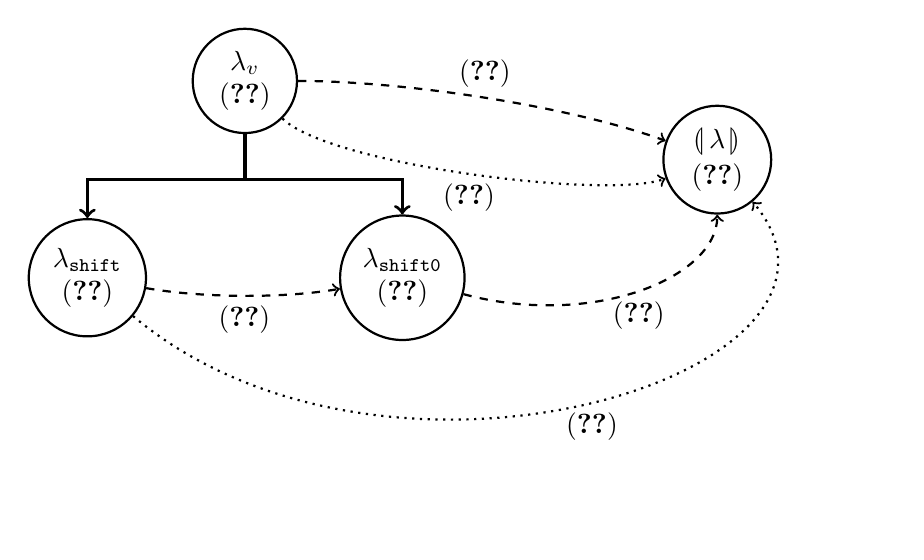
\begin{tikzpicture}[align=center,thick]
    \node[draw,circle](lambda) at (0,0){\shortstack{$\lambda_v$ \\ (\ref{sec:introducing-cbv})}};
    \node[draw,circle](shift) at +(-2,-2.5){\shortstack{$\lambda_\shift$ \\ (\ref{sec:turning-to-shift})}};
    \node[draw,circle](shift0) at +(2,-2.5){\shortstack{$\lambda_\shifto$ \\ (\ref{sec:introducing-control-operators})}};
    \node[draw,circle](banana) at +(6,-1){\shortstack{$\banana{\lambda}$ \\ (\ref{chap:definitions})}};
    \coordinate(split) at +(0,-1.25);
    \draw[very thick] (lambda) -- (split);
    \draw[->,very thick] (split) -| (shift);
    \draw[->,very thick] (split) -| (shift0);
    \draw[->,dashed] (lambda) .. controls +(0:2) and +(160:2) .. (banana) node[midway,above]{(\ref{sec:simulating-cbv})};
    \draw[->,dotted] (lambda) .. controls +(-45:1.5) and +(-160:1.5) .. (banana) node[midway,below]{(\ref{sec:simulating-cbv})};
    \draw[->,dashed] (shift0) .. controls +(-15:2.5) and +(270:1.5) .. (banana) node[midway,below]{(\ref{sec:simulating-shift0})};
    \draw[->,dashed] (shift) .. controls +(-10:1.5) and +(190:1.5) .. (shift0) node[midway,below]{(\ref{sec:turning-to-shift})};
    \draw[->,dotted] (shift) .. controls +(-40:5) and +(-50:3.5) .. (banana) node[midway,below]{(\ref{sec:considering-types})};
  \end{tikzpicture}
  \end{center}
  \caption[The plan of
  Chapter~\ref{chap:continuations}.]{\label{fig:continuation-plan} The plan
    of Chapter~\ref{chap:continuations}. The nodes are calculi, solid edges
    correspond to extensions of calculi, dashed edges correspond to
    translations of rewriting relations and dotted edges correspond to
    translations of type systems.}
\end{figure}


%% \begin{figure}
%%   \includegraphics[width=\textwidth]{diagrams/continuations.pdf}
%%   \caption{\label{fig:cont-diagram} The different calculi we will study in
%%     this section and their relationships.}
%% \end{figure}

\minitoc

\section{Introducing Call-by-Value}
\label{sec:introducing-cbv}

The nature of control operators is that their evaluation depends on their
context. In order for a language with such control operators to be
deterministic, it must have a fixed evaluation order. So in order to set up
the stage for our study of delimited control, we will start by simulating
the call-by-value $\lambda$-calculus in $\banana{\lambda}$.

First, we introduce some key notions of call-by-value and ordered
evaluation in the call-by-value $\lambda$-calculus.

We will single out some of the terms in $\lambda_v$ and call them values.

\begin{definition}
  The following grammar defines the \demph{terms} of $\lambda_v$
  (metavariables $M$ and $N$) and the \demph{values} (metavariable $V$).

\begin{align*}
  V ::= &\ \lam{x}{M} \\
   | \, &\ x \\
  M, N ::= &\ V \\
   | \, &\ (\ap{M}{N})
\end{align*}
\end{definition}

The idea behind this distinction is that values ($V$) are terms that have
already been reduced/evaluated. This distinction will become useful in
definining the following notion:

\begin{definition}
  We define an \demph{evaluation context} $C$ as a structure formed by the
  following grammar:

\begin{align*}
  C ::= &\ [] \\
  | \, &\ (\ap{C}{M}) \\
  | \, &\ (\ap{V}{C})
\end{align*}

  We write $C[M]$ to designate the term that you obtain by replacing the
  $[]$ in $C$ with $M$.
\end{definition}

We now have all the pieces in play to be able to define the semantics of
$\lambda_v$.

\begin{definition}
  A term $M$ \demph{reduces to} a term $N$ in one step, written as $M \to
  N$, when the pair $M \to N$ matches this pattern:

$$
C[\ap{(\lam{x}{M})}{V}] \to_\beta C[\subst{M}{x}{V}]
$$
\end{definition}

Here we see that we only substitute \emph{values} for the variables in a
$\lambda$-abstraction. Also note that we can only perform reductions inside
an evaluation context. Given our definition of $C$, this enforces a
left-to-right evaluation order and also prohibits evaluation under a
$\lambda$-abstraction.


\section{Simulating Call-by-Value}
\label{sec:simulating-cbv}

We first present the translation from $\lambda_v$ to $\banana{\lambda}$ and
then we elaborate on it.

\begin{definition}
  Let $M$ be a term of $\lambda_v$. We define its \demph{interpretation} in
  $\banana{\lambda}$, written as $\sem{M}$:

\begin{align*}
  \sem{x} &= \ap{\eta}{x} \\
  \sem{\lam{x}{M}} &= \ap{\eta}{(\lam{x}{\sem{M}})} \\
  \sem{\ap{M}{N}} &= \sem{M} \hsbind (\lam{m}{\sem{N} \hsbind (\lam{n}{\ap{m}{n}})})
\end{align*}
\end{definition}

An expression of $\lambda_v$ is modelled in $\banana{\lambda}$ as a
computation. The values form a special case since they are all interpreted
as pure computations, terms of the form $(\ap{\eta}{M})$ for some $M$. In
interpreting an application $(\ap{M}{N})$, we first evaluate $M$ and then
$N$, reflecting the behavior we have defined for $\lambda_v$ above.

Before we show that this translation is indeed a faithful one, we will
discuss the types of the interpretations to get a better understanding of
the structures involved.

$\lambda_v$ can be typed with the type system of the simply-typed
$\lambda$-calculus. A well-typed $\lambda_v$ term will then yield a
well-typed $\banana{\lambda}$ term since our translation satisifies the
following property. 

\begin{property}
  Let $M$ be $\lambda_v$ term, $\alpha$ a simple type, $\Gamma$ a
  simply-typed environment and $E$ an effect signature. Then the following
  implication holds.

$$
\Gamma \vdash M : \alpha
\quad \Rightarrow \quad
\sem{\Gamma} \vdash \sem{M} : \FF_E(\sem{\alpha})
$$
\end{property}

\begin{proof}
  By structural induction on the structure of $M$. The
  Definition~\ref{def:cont-interpret-types} of $\sem{.}$ for simple types
  and simply-typed environments is given just below.
\end{proof}

\begin{definition}\label{def:cont-interpret-types}
We define the \demph{interpretation of types and environments} using the
following formulas. $\nu$ stands for an atomic type and $\emptyset$ for the
empty environment.

\begin{align*}
  \sem{\alpha \to \beta} &= \sem{\alpha} \to \FF_E(\sem{\beta}) \\
  \sem{\nu} &= \nu \\
  \sem{\Gamma, x: \alpha} &= \sem{\Gamma}, x: \sem{\alpha} \\
  \sem{\emptyset} &= \emptyset
\end{align*}
\end{definition}

We see that we model $\lambda_v$ expressions of type $\alpha$ using
computations that yield values of type $\sem{\alpha}$. $\sem{.}$ translates
the function type so that it takes values but produces computations (since
the body of a $\lambda$-abstraction can in general be any expression and
the denotation of an expression is a computation).

To show that our translation simulates the behavior of $\lambda_v$, we will
prove that any reduction chain $M \tto N$ in $\lambda_v$ gives rise to a
reduction chain $\sem{M} \tto \sem{N}$ in $\banana{\lambda}$. We start by
proving $\sem{\ap{(\lam{x}{M})}{V}} \tto \sem{\subst{M}{x}{V}}$.

\begin{property}
  Let $M$ be a $\lambda_v$ term and $V$ a $\lambda_v$ value. Then the
  following reduction chain exists in $\calc$:
  
  $\sem{\ap{(\lam{x}{M})}{V}} \tto \sem{\subst{M}{x}{V}}$
\end{property}

\begin{proof}

\NoChapterPrefix
\begin{align}
  \sem{\ap{(\lam{x}{M})}{V}}
&= \sem{\lam{x}{M}} \hsbind (\lam{m}{\sem{V} \hsbind (\lam{n}{\ap{m}{n}})}) \\
&= (\ap{\eta}{(\lam{x}{\sem{M}})}) \hsbind (\lam{m}{(\ap{\eta}{v}) \hsbind (\lam{n}{\ap{m}{n}})}) \\
&\to_{\eta.\hsbind,\beta} (\ap{\eta}{v}) \hsbind (\lam{n}{\ap{(\lam{x}{\sem{M}})}{n}}) \\
&\to_{\eta.\hsbind,\beta} \ap{(\lam{x}{\sem{M}})}{v} \\
&\to_{\beta} \subst{\sem{M}}{x}{v} \\
&= \sem{\subst{M}{x}{V}}
\end{align}
\setcounter{equation}{0}
\ChapterPrefix

where $\sem{V} = \ap{\eta}{v}$. We first expand the definition of $\sem{.}$
for the application, the abstraction and the argument value (we note that
$\sem{V}$ is always equal to $\ap{\eta}{v}$ for some $v$). Since we have
two occurrences of a pure computation being piped into a bind
($(\ap{\eta}{x}) \hsbind k$), we can simplify using $\eta.\hsbind$ and
$\beta$. On line 5, we finally get to the point where we perform the
$\banana{\lambda}$ $\beta$-reduction that actually corresponds to the
$\lambda_v$ $\beta$-reduction that we are modelling.

On line 6, we push the substitution under the $\sem{.}$ operator. This is
valid, since any free $x$ in $\sem{M}$ must have originated as a
translation of a free $x$ in $M$. In the first expression, such an $x$
would get interpreted as $\ap{\eta}{x}$ and then $x$ would get replaced
with $v$ to get $\ap{\eta}{v}$. In the second expression, the $x$ would
first get replaced by $V$ and then $V$ would be interpreted as
$\ap{\eta}{v}$. In both cases, we get the same result.

\end{proof}

We have proven that our simulation preserves the reduction
$\ap{(\lam{x}{M})}{V} \to \subst{M}{x}{V}$. However, it might seem that our
work is not over since this is just a special case of the rule in
$\lambda_v$, which licenses the reduction
$C[\ap{(\lam{x}{M})}{V}] \to C[\subst{M}{x}{V}]$. Nevertheless, our
calculus is pure and lets us perform reductions in any syntactic context
(see the notion of context closure from~\ref{sec:reductions}). This means
that whenever we have $\sem{M} \to \sem{N}$, we also always have
$\sem{C}[\sem{M}] \to \sem{C}[\sem{N}]$,\footnote{We have not defined the
  $\sem{.}$ interpretation operator for contexts. Contexts are simply terms
  with a $[]$ inside and so we just extend the $\sem{.}$ interpretation of
  terms with the clause $\sem{[]} = []$.} which is the same as
$\sem{C[M]} \to \sem{C[N]}$.

\begin{corollary}
  Let $M$ and $N$ be terms of $\lambda_v$ such that $M \tto N$. Then we
  have that $\sem{M} \tto \sem{N}$ in $\banana{\lambda}$.
\end{corollary}

We have shown that our translation \emph{preserves} reduction chains. Can
we get anything stronger?

The inverse is not true in this case. Consider the example of
$M = \lam{x}{(\ap{(\lam{y}{y})}{x})}$ and $N = \lam{x}{x}$. If we take
$\sem{M}$ and perform some reductions, we arrive at
$\ap{\eta}{(\lam{x}{\ap{\eta}{x}})}$. However, this is equal to $\sem{N}$
and so we have $\sem{M} \tto \sem{N}$. This is the case even though $M$
does not reduce to $N$ in $\lambda_v$ ($\lambda_v$ does not allow
reductions inside a $\lambda$-abstraction). Our interpretation will end up
licencing an equality between $M$ and $N$ even though the language we were
modelling ($\lambda_v$) does not equate them (in a way, this interpretation
is complete but not sound). While this makes the interpretation less
appealing, we still elaborate it because it is instructive in showing the
similarity between delimited control and effect handlers.

To conclude this section, we have defined a translation from $\lambda_v$
to $\banana{\lambda}$ and proven that it preserves types and
reductions. This means that we have a way of simulating simply-typed
$\lambda_v$ in our typed $\banana{\lambda}$ and a way of simulating untyped
$\lambda_v$ in an untyped version of $\banana{\lambda}$.

\section{Introducing Control Operators}
\label{sec:introducing-control-operators}

Now that we have introduced how a $\lambda$-calculus with a notion of
evaluation order is to be interpreted in $\banana{\lambda}$, we are ready
to introduce control operators. Our claim is that the effects and handlers
of $\calc$ are very close to delimited continuations.\footnote{This analogy
  originates with Andrej Bauer who says that effects and handlers are to
  delimited continuations what while loops or if-then-else statements are
  to gotos~\cite{bauer2012lambda}.} The pair of operators that resembles
the behavior of handlers the most are the operators $\shifto$ and
$\reseto$.

\begin{definition}
  We define the \demph{terms} ($M$, $N$) and values $V$ of
  $\lambda_\shifto$ using the following grammar:

\begin{align*}
  V ::= &\ \lam{x}{M} \\
   | \, &\ x \\
  M, N ::= &\ V \\
   | \, &\ (\ap{M}{N}) \\
   | \, &\ (\ap{\shifto}{M}) \\
   | \, &\ (\ap{\reseto}{M})
\end{align*}
\end{definition}

The terms of this new calculus, $\lambda_{\shifto}$, are just the terms of
$\lambda_v$ extended with the operators $\shifto$ and $\reseto$. Before we
give the reduction rules, we will also have to refine our notion of an
evaluation context.

\begin{definition}
  We define \demph{evaluation contexts} ($C$) and \demph{evaluation frames}
  ($F$) the following way:
\begin{align*}
  C ::= &\ [] \\
   | \, &\ (\ap{C}{M}) \\
   | \, &\ (\ap{V}{C}) \\
   | \, &\ (\ap{\shifto}{C}) \\
   | \, &\ (\ap{\reseto}{C}) \\
  F ::= &\ [] \\
   | \, &\ (\ap{F}{M}) \\
   | \, &\ (\ap{V}{F}) \\
   | \, &\ (\ap{\shifto}{F})
\end{align*}
\end{definition}

For evaluation contexts ($C$), we add rules saying that when evaluating
applications of either $\shifto$ or $\reseto$, we can evaluate their
arguments. We also introduce a notion of an evaluation frame
($F$). Similarly to how values are a subset of terms, evaluation frames are
a subset of evaluation contexts. A frame is a context which does not embed
$[]$ inside a $\reseto$.

\begin{definition}
  A term $M$ \demph{reduces to} a term $N$ in $\lambda_\shifto$ in one step
  whenever $M$ and $N$ match one of the patterns below:

\vspace{4mm}
\begin{tabular}{>{$}r<{$} >{$}c<{$} >{$}l<{$}}
  C[\ap{(\lam{x}{M})}{V}] & \to_\beta & C[\subst{M}{x}{V}] \\
  C[\ap{\reseto}{V}] & \to_{\reseto} & C[V] \\
  C[\ap{\reseto}{(F[\ap{\shifto}{V}])}] & \to_{\shifto} & C[\ap{V}{(\lam{x}{\ap{\reseto}{(F[x])}})}]
\end{tabular}
\vspace{4mm}
\end{definition}

We keep the reduction rule $\beta$ and we add two new rules for $\reseto$
and $\shifto$. The rule for $\reseto$ makes $\reseto$ look redundant but
its importance shows up in the rule for $\shifto$. In the $\shifto$ rule,
we have an application of $\shifto$ buried inside the context
$C[\ap{\reseto}{F}]$. This kind of context corresponds to a context which
embeds $[]$ inside at least one $\reseto$. The $F$ then corresponds to the
frame which separates the $\shifto$ from the nearest enclosing
$\reseto$. The only role of $\reseto$ is thus to serve as a kind of marker
to delimit the context/continuation $F$ of $\shifto$. The argument to
$\shifto$ then receives this continuation $F$, composed with $\reseto$, as
its argument.\footnote{You may already start to see similarities with the
  $\banana{\op{op}}$ rule of $\banana{\lambda}$ and why we chose $\shifto$
  and $\reseto$ in particular.}

\section{Simulating $\shifto$ and $\reseto$}
\label{sec:simulating-shift0}

To simulate $\lambda_{\shifto}$ in $\banana{\lambda}$, all we have to do is
extend the simulation of $\lambda_v$ with interpretations of the two new
syntactic forms.

\begin{definition}
  Let $M$ be a term of $\lambda_\shifto$. We define its
  \demph{interpretation} $\sem{M}$ as an extension of the interpretation
  defined for $\lambda_v$ with the following clauses:

\begin{align*}
  \sem{\ap{\shifto}{M}} &= \sem{M} \hsbind (\lam{m}{\ap{\op{shift0}!}{m}}) \\
  \sem{\ap{\reseto}{M}} &= \ap{\resetobanana}{\sem{M}}
\end{align*}
\end{definition}

The above translation also gives us a general template for simulating
effectful calculi in $\banana{\lambda}$. Amongst the impure operators of a
calculus, we identify those that manipulate a context (raising an
exception, modifying a variable, reading a dynamically bound value,
accessing the continuation\ldots) and those that establish a context
(exception handlers, transactions, binders for dynamic variables,
continuation delimiters such as $\texttt{prompt}$ or
$\texttt{reset}$\ldots). Operators that manipulate the context are
translated into operations in $\banana{\lambda}$,
i.e.\ $\sem{\ap{\texttt{op}}{M}} = \sem{M} \hsbind
(\lam{m}{\ap{\op{op}!}{m}})$. Operators that establish a context are
translated into handlers, i.e.\ $\sem{\ap{\texttt{op}}{M}} =
\ap{\banana{\ldots}}{\sem{M}}$.

To show that this simulation is faithful, we will prove that $M \to N$ in
$\lambda_{\shifto}$ implies $\sem{M} \ttoffrom \sem{N}$ in
$\banana{\lambda}$. $\sem{M} \ttoffrom \sem{N}$ says that we can go from
$\sem{M}$ to $\sem{N}$ through a series of reductions and expansions, i.e.\
$\sem{M}$ and $\sem{N}$ are convertible.\footnote{We will need the
  expansions when ``unevaluating'' some of the monadic binds that have been
  introduced by our translations.} In this case, our simulation property
will prove that equivalence given by the calculus' equational theory is
preserved,
% \footnote{Such a one-sided property is also satisfied by trivial
% interpretations so the property itself does not do the interpretation
% justice. In other words, this interpretation is complete but not sound
% (consider already the $\lambda_v$ example towards the end of
% \ref{sec:simulating-cbv}). Is there some better characterization of this
% kind of simulation? Check out Plotkin's seminal paper on Call-by-value,
% call-by-name and the lambda-calculus.}
i.e.\ $M = N$ in $\lambda_\shifto$ implies $\sem{M} = \sem{N}$ in
$\banana{\lambda}$ (where $X = Y$ is to be read as $X \ttoffrom Y$).

\begin{property}
  Let $M$ and $N$ be terms of $\lambda_\shifto$. If $M \to N$, then
  $\sem{M} \ttoffrom \sem{N}$.
\end{property}

\begin{proof}
We have three reduction rules to tackle: $\to_\beta$, $\to_\reseto$ and
$\to_\shifto$. We have proven the case of $\to_\beta$
in~\ref{sec:simulating-cbv} and that proof still holds in this extended
interpretation. We also reuse our observation
from~\ref{sec:simulating-cbv} that in order to prove $\sem{C[M]} \tto
\sem{C[N]}$, it is enough to prove $\sem{M} \tto \sem{N}$. The case of
$\to_\reseto$ is a simple one so we will deal with that first:

\NoChapterPrefix
\begin{align}
  \sem{\ap{\reseto}{V}}
  &= \ap{\resetobanana}{\sem{V}} \\
  &= \ap{\resetobanana}{(\ap{\eta}{v})} \\
  &\to_{\banana{\eta}} \ap{\eta}{v} \\
  &= \sem{V}
\end{align}
\setcounter{equation}{0}
\ChapterPrefix

where $\sem{V} = \ap{\eta}{v}$. As we have said
in~\ref{ssec:operations-and-handlers}, an (open) handler without an
explicit clause for $\eta$ is presumed to handle $\eta$ with $\eta$. In
this case, the $\lambda_\shifto$ reduction ends up corresponding to exactly
one $\banana{\eta}$ reduction in $\banana{\lambda}$.

Now, let's deal with the last reduction rule, $\to_\shifto$.

\NoChapterPrefix
\begin{align}
  \sem{\ap{\reseto}{(F[\ap{\shifto}{V}])}}
  &= \ap{\resetobanana}{\sem{F[\ap{\shifto}{V}]}} \\
  &\ttoffrom \ap{\resetobanana}{(\app{\op{shift0}}{v}{(\lam{x}{\sem{F[x]}})})} \\
  &\to_{\banana{\op{op}}} \app{(\lam{c k}{\ap{c}{k}})}{v}{(\lam{x}{\ap{\resetobanana}{\sem{F[x]}}})} \\
  &\to_{\beta,\beta} \ap{v}{(\lam{x}{\ap{\resetobanana}{\sem{F[x]}}})} \\
  &= \ap{v}{(\lam{x}{\sem{\ap{\reseto}{(F[x])}}})} \\
  &\from_{\beta,\eta.\hsbind} (\ap{\eta}{(\lam{x}{\sem{\ap{\reseto}{(F[x])}}})}) \hsbind (\lam{n}{\ap{v}{n}}) \\
  &= \sem{\lam{x}{\ap{\reseto}{(F[x])}}} \hsbind (\lam{n}{\ap{v}{n}}) \\
  &\from_{\beta,\eta.\hsbind} (\ap{\eta}{v}) \hsbind (\lam{m}{\sem{\lam{x}{\ap{\reseto}{(F[x])}}} \hsbind (\lam{n}{\ap{m}{n}})}) \\
  &= \sem{V} \hsbind (\lam{m}{\sem{\lam{x}{\ap{\reseto}{(F[x])}}} \hsbind (\lam{n}{\ap{m}{n}})}) \\
  &= \sem{\ap{V}{(\lam{x}{\ap{\reseto}{(F[x])}})}}
\end{align}
\setcounter{equation}{0}
\ChapterPrefix

where $\sem{V} = \ap{\eta}{v}$. Lines 2 and 3 are the crucial lines. On
line 2, we use the upcoming Lemma~\ref{lem:contexts-continuations} that
will show that through a series of reductions and expansions, we can go
from $\sem{F[\ap{\shifto}{V}]}$ to
$(\app{\op{shift0}}{v}{(\lam{x}{\sem{F[x]}})})$ where $\sem{V} =
\ap{\eta}{v}$. Since we have moved $\op{shift0}$ to the head of the
handler's argument, we can apply the $\banana{\op{op}}$ rule on line
3. Since the handler clause is basically the identity function, it
disappears on line 4 after two $\beta$-reductions.

From then on, we perform a series of expansions while trying to push the
interpretation operator $\sem{.}$ outwards from $F[x]$ to the entire
expression. The expansions used above are a reversal of a common idiom we
have used before. We used to go from $(\ap{\eta}{M}) \hsbind (\lam{m}{N})$
to $\subst{N}{m}{M}$ using $\eta.\hsbind$ and then a
$\beta$-reduction. Here, we go the other way from $\subst{N}{m}{M}$ to
$(\ap{\eta}{M}) \hsbind (\lam{m}{N})$ using a $\beta$-expansion and the
derived expansion $\eta.\hsbind$ (lines 6 and 8).
\end{proof}

\begin{corollary}
  \label{coro:simul-sem}
  Let $M$ and $N$ be terms of $\lambda_\shifto$. If $M \ttoffrom N$ in
  $\lambda_\shifto$, then $\sem{M} \ttoffrom \sem{N}$ in
  $\banana{\lambda}$.
\end{corollary}


\subsection*{Contexts $=$ Continuations: Proving the Lemma}

All that is left to show is a proof of the lemma we mentioned above.

\begin{lemma}
\label{lem:contexts-continuations}
$$
\sem{F[\ap{\shifto}{V}]} \ttoffrom (\app{\op{shift0}}{v}{(\lam{x}{\sem{F[x]}})})
$$

where $\sem{V} = \ap{\eta}{v}$. 
\end{lemma}

This lemma not only allows us to prove the simulation property that is the
focus of this section, but it also gives us more insight into
$\banana{\lambda}$. If we read it from right to left and slightly
generalizing, it tells us how to think of terms of the form
$(\app{\op{op}}{x}{k})$. They represent computations where the next point
of evaluation is a contextually dependent operation $\op{op}$: $x$ is the
operation's argument and $k$ captures the context in which $\op{op}$ is
being used inside the computation.

\begin{proof}
Our proof will proceed by induction on the structure of $F$. We will start
with the base case, $F = []$.

\NoChapterPrefix
\begin{align}
  \sem{F[\ap{\shifto}{V}]}
  &= \sem{\ap{\shifto}{V}} \\
  &= \sem{V} \hsbind (\lam{m}{\ap{\op{shift0}!}{m}}) \\
  &\to_{\eta.\hsbind,\beta} \ap{\op{shift0}!}{v} \\
  &= \ap{(\lam{p}{\app{\op{shift0}}{p}{(\lam{x}{\etaE{x}}}})}{v} \\
  &\to_\beta \app{\op{shift0}}{v}{(\lam{x}{\etaE{x}})} \\
  &= \app{\op{shift0}}{v}{(\lam{x}{\sem{x}})} \\
  &= \app{\op{shift0}}{v}{(\lam{x}{\sem{F[x]}})}
\end{align}
\setcounter{equation}{0}
\ChapterPrefix

The individual steps are pretty self-explanatory. On line 4, we expand the
definition of the exclamation mark from~\ref{ssec:operations-and-handlers}.

Next case, $F = (\ap{F'}{M})$:

\NoChapterPrefix
\begin{align}
  \sem{F[\ap{\shifto}{V}]}
  &= \sem{\ap{(F'[\ap{\shifto}{V}])}{M}} \\
  &= \sem{F'[\ap{\shifto}{V}]} \hsbind (\lam{m}{\sem{M} \hsbind (\lam{n}{\ap{m}{n}})}) \\
  &\ttoffrom (\app{\op{shift0}}{v}{(\lam{x}{\sem{F'[x]}})}) \hsbind (\lam{m}{\sem{M} \hsbind (\lam{n}{\ap{m}{n}})}) \\
  &\to_{\op{op}.\hsbind} \app{\op{shift0}}{v}{(\lam{x}{\sem{F'[x]} \hsbind (\lam{m}{\sem{M} \hsbind (\lam{n}{\ap{m}{n}})})})} \\
  &= \app{\op{shift0}}{v}{(\lam{x}{\sem{\ap{(F'[x])}{M}}})} \\
  &= \app{\op{shift0}}{v}{(\lam{x}{\sem{F[x]}})} \\
\end{align}
\setcounter{equation}{0}
\ChapterPrefix

Again, the steps are quite mechanical. Line 3 uses the induction hypothesis
and on line 4, we see the derived $\op{op}.\hsbind$ rule introduced in
~\ref{ssec:bind} pushing the $\hsbind$ inside the continuation.

Case $F = (\ap{V'}{F'})$:

\NoChapterPrefix
\begin{align}
  \sem{F[\ap{\shifto}{V}]}
  &= \sem{\ap{V'}{(F'[\ap{\shifto}{V}])}} \\
  &= \sem{V'} \hsbind (\lam{m}{\sem{F'[\ap{\shifto}{V}]} \hsbind (\lam{n}{\ap{m}{n}})}) \\
  &\to_{\eta.\hsbind,\beta} \sem{F'[\ap{\shifto}{V}]} \hsbind (\lam{n}{\ap{v'}{n}}) \\
  &\ttoffrom (\app{\op{shift0}}{v}{(\lam{x}{\sem{F'[x]}})}) \hsbind (\lam{n}{\ap{v'}{n}}) \\
  &\to_{\op{op}.\hsbind} \app{\op{shift0}}{v}{(\lam{x}{\sem{F'[x]} \hsbind (\lam{n}{\ap{v'}{n}})})}\\
  &\from_{\beta,\eta.\hsbind} \app{\op{shift0}}{v}{(\lam{x}{\sem{V'} \hsbind (\lam{m}{\sem{F'[x]} \hsbind (\lam{n}{\ap{m}{n}})})})}\\
  &= \app{\op{shift0}}{v}{(\lam{x}{\sem{\ap{V'}{(F'[x])}}})} \\
  &= \app{\op{shift0}}{v}{(\lam{x}{\sem{F[x]}})}
\end{align}
\setcounter{equation}{0}
\ChapterPrefix

where $\sem{V'} = \ap{\eta}{v'}$. This proof is very similar to the one for
the case before. We have just two extra steps, on lines 3 and 6, where we
first push the $\sem{V'}$ ($= \ap{\eta}{v'}$) in through the $\hsbind$
using $\eta.\hsbind$ and $\beta$ and then we pull it out in a different
context by reversing the process.

Finally, the last case, where $F = (\ap{\shifto}{F'})$:

\NoChapterPrefix
\begin{align}
  \sem{F[\ap{\shifto}{V}]}
  &= \sem{\ap{\shifto}{(F'[\ap{\shifto}{V}])}} \\
  &= \sem{F'[\ap{\shifto}{V}]} \hsbind (\lam{m}{\ap{\op{shift0}!}{m}}) \\
  &\ttoffrom (\app{\op{shift0}}{v}{(\lam{x}{\sem{F'[x]}})}) \hsbind (\lam{m}{\ap{\op{shift0}!}{m}}) \\
  &\to_{\op{op}.\hsbind} \app{\op{shift0}}{v}{(\lam{x}{\sem{F'[x]} \hsbind (\lam{m}{\ap{\op{shift0}!}{m}})})} \\
  &= \app{\op{shift0}}{v}{(\lam{x}{\sem{\ap{\shifto}{(F'[x])}}})} \\
  &= \app{\op{shift0}}{v}{(\lam{x}{\sem{F[x]}})}
\end{align}
\setcounter{equation}{0}
\ChapterPrefix

And this case is just as simple as the $F = (\ap{F'}{M})$ one. This
concludes our proof of this lemma. Note that we did not include a case for
$F = (\ap{\reseto}{F'})$. Such a context is not a frame, since it embeds
$[]$ inside a $\reseto$. We can also check that our property would no
longer hold in this case, since the $\shifto$ coming from $F'$ would get
handled by the $\reseto$.
\end{proof}

By proving this lemma, we have also finished our proof of the fact that
whenever we have $M \ttoffrom N$ in $\lambda_\shifto$, we also have
$\sem{M} \ttoffrom \sem{N}$ in $\banana{\lambda}$.


\section{Turning to $\shift$ and $\reset$}
\label{sec:turning-to-shift}

There are other control operators, similar to $\shifto$ and $\reseto$. One
example would be the more common $\shift$ and $\reset$. The difference
between these two pairs can be appreciated by comparing the reduction rules
for $\shifto$ and $\shift$.

\vspace{4mm}
\begin{tabular}{>{$}r<{$} >{$}c<{$} >{$}l<{$}}
  C[\ap{\reseto}{(F[\ap{\shifto}{V}])}] & \to_{\shifto} & C[\ap{V}{(\lam{x}{\ap{\reseto}{(F[x])}})}] \\
  C[\ap{\reset}{(F[\ap{\shift}{V}])}] & \to_{\shift} & C[\ap{\reset}{(\ap{V}{(\lam{x}{\ap{\reset}{(F[x])}})})}]
\end{tabular}
\vspace{4mm}

$\shift$ preserves the delimiting $\reset$ and installs a new one into the
continuation. $\shifto$ is different in that it removes the delimiting
$\reseto$. In all other ways, the definition of $\lambda_\shift$ (the
call-by-value $\lambda$-calculus equipped with $\shift$ and $\reset$) is
identical to the one of $\lambda_\shifto$.

We have seen that the semantics of $\shifto$ and $\reseto$ aligns closely
with the behavior of operations and handlers in
$\banana{\lambda}$. However, we can translate $\shift$ and $\reset$ to
$\banana{\lambda}$ too.

We will do so by first translating $\lambda_\shift$ to $\lambda_\shifto$.

\begin{definition}
  The \demph{interpretation} $\semo{M}$ of a $\lambda_\shift$ term $M$ into
  $\lambda_\shifto$ is defined as follows:

  \begin{align*}
    \semo{\ap{\reset}{M}} &= \ap{\reseto}{\semo{M}} \\
    \semo{\ap{\shift}{M}} &= \ap{\shifto}{(\ap{(\lam{m}{\lam{k}{\ap{\reseto}{(\ap{m}{k})}}})}{\semo{M}})} \\
    \semo{\ap{M}{N}} &= \ap{\semo{M}}{\semo{N}} \\
    \semo{\lam{x}{M}} &= \lam{x}{\semo{M}} \\
    \semo{x} &= x
  \end{align*}

\end{definition}

NB: We cannot use
$(\ap{\shifto}{(\lam{k}{\ap{\reseto}{(\ap{\semo{M}}{k})}})})$ for the
interpretation of $\sem{\ap{\shift}{M}}$. That would result in
$\semo{(\ap{\shift}{[]})}$ being equal to
$(\ap{\shifto}{(\lam{k}{\ap{\reseto}{(\ap{[]}{k})}})})$. The problem here
is that $(\ap{\shift}{[]})$ is an evaluation frame in $\lambda_\shift$, but
its interpretation is not even an evaluation context in $\lambda_\shifto$
since the $[]$ is buried under a $\lambda$-abstraction.

To see that this interpretation preserves the same kind of property we have
been demonstrating in the rest of this section, we prove the following.

\begin{property}
  \label{prop:simul-semo}
  For any $\lambda_\shift$ terms $M$ and $N$, $M \to N$ implies $\semo{M}
  \tto \semo{N}$.
\end{property}

\begin{proof}
  We first note that if $C$ is an evaluation context in $\lambda_\shift$,
  $\semo{C}$ (where $\semo{.}$ has been extended to contexts with
  $\semo{[]} = []$) is an evaluation context in $\lambda_\shifto$. The same
  also holds for evaluation frames and values. With these observations in
  our hand, we can proceed onto the proof.

  We consider the three possible cases of $M \to N$ that correspond to the
  three reduction rules in $\lambda_\shift$. Since the rules $\to_\beta$
  and $\to_\reset$/$\to_\reseto$ are identical in both calculi and since
  $\semo{.}$ preserves evaluation contexts and values, these cases fall out
  immediately.

  We only have to handle the interesting case of $M \to_\shift N$. In that
  case, $M = C[\ap{\reset}{(F[\ap{\shift}{V}])}]$ and $N =
  C[\ap{\reset}{(\ap{V}{(\lam{x}{\ap{\reset}{(F[x])}})})}]$ for some
  context $C$, frame $F$ and value $V$.

  \NoChapterPrefix
  \begin{align}
    \semo{M} &= \semo{C[\ap{\reset}{(F[\ap{\shift}{V}])}]} \\
             &= C'[\ap{\reseto}{(F'[\ap{\shifto}(\ap{(\lam{m}{\lam{k}{\ap{\reseto}{(\ap{m}{k})}}})}{V'})])}] \\
             &\to_\beta C'[\ap{\reseto}{(F'[\ap{\shifto}(\lam{k}{\ap{\reseto}{(\ap{V'}{k})}})])}] \\
             &\to_\shifto C'[\ap{(\lam{k}{\ap{\reseto}{(\ap{V'}{k})}})}{(\lam{y}{\ap{\reseto}{(F'[y])}})}] \\
             &\to_\beta C'[\ap{\reseto}{(\ap{V'}{(\lam{y}{\ap{\reseto}{(F'[y])}})})}] \\
             &= \semo{C[\ap{\reset}{(\ap{V}{(\lam{x}{\ap{\reset}{(F[x])}})})}]} \\
             &= \semo{N}
  \end{align}
  \setcounter{equation}{0}
  \ChapterPrefix

  where $C' = \semo{C}$, $F' = \semo{F}$ and $V' = \semo{V}$.
\end{proof}

\begin{corollary}
  \label{coro:simul-semo}
  For any $\lambda_\shift$ terms $M$ and $N$, $M \tto N$ implies $\semo{M}
  \tto \semo{N}$ and $M \ttoffrom N$ implies $\semo{M} \ttoffrom \semo{N}$.
\end{corollary}

\begin{corollary}
  For any $\lambda_\shift$ terms $M$ and $N$, $M \ttoffrom N$ implies
  $\sem{\semo{M}} \ttoffrom \sem{\semo{N}}$ in $\banana{\lambda}$.
\end{corollary}

For the latter corollary, we just compose the translations from
$\lambda_\shift$ to $\lambda_\shifto$ and from $\lambda_\shifto$ to
$\banana{\lambda}$ and transitively apply their simulation properties
(Corollaries~\ref{coro:simul-sem} and~\ref{coro:simul-semo}).

This lets us extend our interpretation $\sem{.}$ to $\lambda_\shift$.

\begin{align*}
  \sem{\ap{\shift}{M}} &= \sem{M} \hsbind (\lam{m}{\ap{\op{shift0}!}{(\lam{k}{\ap{\resetobanana}{(\ap{m}{k})}})}}) \\
  \sem{\ap{\reset}{M}} &= \ap{\resetobanana}{\sem{M}}
\end{align*}

In the sequel, we will be translating a type system of $\lambda_\shift$ to
the type system of $\banana{\lambda}$. For the types to work out in this
translation, we will need to throw a few bananas into the mix. In what will
follow, we will assume that $\shift$ and $\reset$ are translated to
$\banana{\lambda}$ using the interpretations given below:

\begin{align*}
  \sem{\ap{\shift}{M}} &= \sem{M} \hsbind (\lam{m}{\ap{\op{\shift0}!}{(\lam{k}{\ap{\resetobanana}{(\ap{m}{(\banana{} \compop k)})}})}}) \\
  \sem{\ap{\reset}{M}} &= \ap{\banana{}}{(\ap{\resetobanana}{\sem{M}})}
\end{align*}

$\banana{}$ is actually a valid handler. As any other handler without an
explicit clause for $\eta$, it handles $\eta$ with $\eta$. It also handles
all operations with the operations themselves (i.e.\ rule
$\banana{\op{op}'}$). It is therefore an identity function on
computations. However, the most general type that we can infer for
$\banana{}$ is $\FF_E(\alpha) \to \FF_{E'}(\alpha)$ for any $E$ and $E'$
such that $E \subseteq E'$. It can therefore be used as a kind of explicit
weakening operator on computation types.\footnote{This need for explicit
  weakening of computation types could be eliminated by using actual
  polymorphic types.}


\section{Considering Types}
\label{sec:considering-types}

We have shown embeddings of $\lambda_\shifto$ and $\lambda_\shift$ into
$\banana{\lambda}$. In both of these embeddings, we have seen that the
reduction rules in $\banana{\lambda}$ can emulate those of $\lambda_\shift$
and $\lambda_\shifto$. However, we have not defined $\banana{\lambda}$ only
via terms and their reductions, we have also specified a type system. Can
we somehow guarantee that the results of interpreting $\lambda_\shift$ into
$\banana{\lambda}$ are well-typed?

Clearly not without having some kind of type system for
$\lambda_\shift$. Without a type system, we can write a term like
$\lam{x}{\ap{x}{x}}$ whose translation to $\banana{\lambda}$ is impossible
to type. Danvy and Filinski~\cite{danvy1989functional} give a type system
for a calculus with $\shift$ and $\reset$. In their system, typing
judgments have the following form:

$$
\rho, \alpha \vdash E : \tau, \beta
$$

In this schema, $\rho$ stands for a type environment (context $\Gamma$ in
our notation), $E$ is an expression (a term) and $\tau$ is the type of
$E$. The types $\alpha$ and $\beta$ describe the context in which the
expression can occur. If we rewrote $E$ in continuation-passing style, we
would get a term of type $(\tau \to \alpha) \to \beta$. The expression $E$
can access a context whose answer type is $\alpha$ and supplant it by an
answer of type $\beta$.

This kind of type system allows us to write a computation that performs a
series of $\shift$s, each one changing the answer type for the next. If we
wanted to guarantee type safety while allowing this amount of flexibility,
we would need to use indexed effects \cite{andjelkovic2014towards} to track
the answer type as it changes from $\op{shift0}$ to $\op{shift0}$. We will
therefore modify Danvy and Filinski's type system to prohibit continuations
from changing the answer type so as to fit into the capabilities of our
type system.

Our modified type system will have judgments that follow this schema:

$$
\Gamma \pipe \gamma \vdash M : \tau
$$

We switch to our style of notation, $\Gamma$ is a typing context and $M$ is
a term. We give only a single answer type, $\gamma$, written to the left of
the turnstile. We also separate it from the type context with a vertical
bar instead of a comma so as not to be confusing with the notation for
context extension ($\Gamma, x : \alpha$). In continuation-passing style,
the type of the above term $M$ would correspond to
$(\tau \to \gamma) \to \gamma$.

There is one more subtlety to cover before we look at the typing rules
themselves: what are the types?

\begin{definition}
  A \demph{$\lambda_\shift$ type} is either:
  \begin{itemize}
  \item an atomic type $\nu$
  \item a function type $\alpha \xto{\gamma} \beta$ where $\alpha$, $\beta$
    and $\gamma$ are other $\lambda_\shift$ types
  \end{itemize}
\end{definition}

Since the well-typedness of an expression depends on the context in which
it is being evaluated, the function type becomes a bit more complicated. By
embedding an expression inside a $\lambda$-abstraction, we delay its
evaluation. In function application, the context of the application becomes
the context the function body. In other words, if when type checking the
body of a function we assume that the current answer type is $\gamma$, then
when we apply this function to an argument, we should better do so in a
context in which the answer type actually is $\gamma$. This means we have
to discriminate between functions w.r.t.\ the context (i.e.\ answer type) in
which they can be applied.

\begin{definition}
  We define the \demph{typing relation for $\lambda_\shift$} as the set of all
  judgments derivable from the inference rules given in
  Figure~\ref{fig:typing-rules-shift}.
\end{definition}

\begin{figure}
  \begin{prooftree}
    \AxiomC{$x : \alpha \in \Gamma$}
    \RightLabel{[var]}
    \UnaryInfC{$\Gamma \pipe \gamma \vdash x : \alpha$}
  \end{prooftree}
  
  \begin{subfigure}{.5\textwidth}
    \begin{prooftree}
      \AxiomC{$\Gamma, x : \alpha \pipe \gamma \vdash M : \beta$}
      \RightLabel{[abs]}
      \UnaryInfC{$\Gamma \pipe \delta \vdash \lam{x}{M} : \alpha \xto{\gamma} \beta$}
    \end{prooftree}
  \end{subfigure}
  \begin{subfigure}{.5\textwidth}
    \begin{prooftree}
      \AxiomC{$\Gamma \pipe \gamma \vdash M : \alpha \xto{\gamma} \beta$}
      \AxiomC{$\Gamma \pipe \gamma \vdash N : \alpha$}
      \RightLabel{[app]}
      \BinaryInfC{$\Gamma \pipe \gamma \vdash \ap{M}{N} : \beta$}
    \end{prooftree}
  \end{subfigure}

  \begin{subfigure}{.5\textwidth}
    \begin{prooftree}
      \AxiomC{$\Gamma \pipe \gamma \vdash M : \gamma$}
      \RightLabel{[$\reset$]}
      \UnaryInfC{$\Gamma \pipe \delta \vdash \ap{\reset}{M} : \gamma$}
    \end{prooftree}
  \end{subfigure}
  \begin{subfigure}{.5\textwidth}
    \begin{prooftree}
      \AxiomC{$\Gamma \pipe \gamma \vdash M : (\alpha \xto{\delta} \gamma)
        \xto{\gamma} \gamma$}
      \RightLabel{[$\shift$]}
      \UnaryInfC{$\Gamma \pipe \gamma \vdash \ap{\shift}{M} : \alpha$}
    \end{prooftree}
  \end{subfigure}

  \caption{\label{fig:typing-rules-shift} Typing rules for
    $\lambda_\shift$.}
\end{figure}

To convince ourselves that this type system works, we will need to prove
its soundess by way of demonstrating type preservation and progress.

\begin{lemma}
  \label{lem:subst-shift}
  \demph{Substitution and types in $\lambda_\shift$}

  Whenever we have $\Gamma, x : \alpha \pipe \gamma \vdash M : \tau$ and
  $\Gamma \pipe \gamma \vdash V : \alpha$, we also get $\Gamma \pipe \gamma
  \vdash \subst{M}{x}{V} : \tau$ (i.e.\ we can substitute in $M$ while
  preserving the type).
\end{lemma}
\begin{proof}
  This technical lemma, common to most $\lambda$-calculi, is proven by
  induction on the derivation of
  $\Gamma, x : \alpha \pipe \gamma \vdash M : \tau$ (which is the same as
  induction on the syntactic structure of $M$). The only catch here is that
  when we descend into $M$ through $\lambda$-abstractions and $\reset$s, we
  might be forced to change the answer type from $\gamma$ to some
  $\delta$. Now, in order for the induction to work, we will need to change
  the answer type in $\Gamma \pipe \gamma \vdash V : \alpha$ from $\gamma$
  to $\delta$ as well. In other words, we need to coerce
  $\Gamma \pipe \gamma \vdash V : \alpha$ to
  $\Gamma \pipe \delta \vdash V : \alpha$.

  This is exactly where the condition that the term $V$ that we are
  substituting must be a value comes into play. If we look at the typing
  rules for values (variables and $\lambda$-abstractions), we see that the
  answer type is completely free and therefore if we can prove
  well-typedness w.r.t.\ one answer type, we also get it for all answer
  types.
\end{proof}

\begin{property}
  \demph{Subject reduction for $\lambda_\shift$}

  Let us have $\Gamma \pipe \gamma \vdash M : \tau$ and $M \to N$. Then
  also $\Gamma \pipe \gamma \vdash N : \tau$.
\end{property}
\begin{proof}
  We will prove this property case by case for each reduction rule of
  $\lambda_\shift$. In the proof, we assume that the context $C$ wrapping
  the redex and the contractum is just the empty context $[]$. By the
  compositionality of the type system, it follows that if $M \to N$
  preserves types, then so does $C[M] \to C[N]$.

  \begin{enumerate}
  \item $M \to_\beta N$

    We know that $M = \ap{(\lam{x}{M'})}{V}$, that $N = \subst{M'}{x}{V}$
    and that the derivation of the type of $M$ looks like the following:

    \begin{prooftree}
      \AxiomC{$\Gamma, x : \alpha \pipe \gamma \vdash M' : \tau$}
      \RightLabel{[abs]}
      \UnaryInfC{$\Gamma \pipe \gamma \vdash \lam{x}{M'} : \alpha \xto{\gamma} \tau$}
      \AxiomC{$\Gamma \pipe \gamma \vdash V : \alpha$}
      \RightLabel{[app]}
      \BinaryInfC{$\Gamma \pipe \gamma \vdash \ap{(\lam{x}{M'})}{V} : \tau$}
    \end{prooftree}

    By applying Lemma~\ref{lem:subst-shift} to the typing derivations of
    $M'$ and $V$, we directly get the typing judgment we need.

  \item $M \to_\reset N$

    We have $M = \ap{\reset}{V}$, $N = V$ and the following derivation:

    \begin{prooftree}
      \AxiomC{$\Gamma \pipe \tau \vdash V : \tau$}
      \RightLabel{[$\reset$]}
      \UnaryInfC{$\Gamma \pipe \gamma \vdash \ap{\reset}{V} : \tau$}
    \end{prooftree}

    If we recover the typing derivation for $V$, we run into the same issue
    as in the proof of Lemma~\ref{lem:subst-shift}. The context has changed
    from answer type $\gamma$ to answer type $\tau$. Again, we rely on the
    fact that the argument to $\reset$ must have been a value in order to
    be able to take the judgment $\Gamma \pipe \tau \vdash M : \tau$ and
    coerce it to a judgment $\Gamma \pipe \gamma \vdash M : \tau$.

  \item $M \to_\shift N$

    We have $M = \ap{\reset}{(F[\ap{\shift}{V}])}$, $N =
    \ap{\reset}{(\ap{V}{(\lam{x}{\ap{\reset}{(F[x])}})})}$.

    \begin{prooftree}
      \AxiomC{$\Gamma \pipe \tau \vdash V : (\alpha \xto{\delta} \tau) \xto{\tau} \tau$}
      \RightLabel{[$\shift$]}
      \UnaryInfC{$\Gamma \pipe \tau \vdash \ap{\shift}{V} : \alpha$}
      \UnaryInfC{$\vdots$ $F[]$ $\vdots$}
      \UnaryInfC{$\Gamma \pipe \tau \vdash F[\ap{\shift}{V}] : \tau$}
      \RightLabel{[$\reset$]}
      \UnaryInfC{$\Gamma \pipe \gamma \vdash \ap{\reset}{(F[\ap{\shift}{V}])} : \tau$}
    \end{prooftree}

    The validity of the above analysis hinges on the fact that the context
    separating the $\reset$ and the $\shift$ is an evaluation frame. If we
    look at the typing rules [app] and [$\shift$], we see that the answer
    types of the subterms are always the same as the answer type of the
    compound term. This is what lets us assume that the answer type of both
    $F[\ap{\shift}{V}]$ and $\ap{\shift}{V}$ is $\tau$.

    From this typing derivation, we will extract the typing judgment of $V$
    and the evaluation frame $F$ that can take a term $M'$ such that
    $\Gamma \pipe \tau \vdash M' : \alpha$ to a term $F[M']$ such that
    $\Gamma \pipe \tau \vdash F[M'] : \tau$.

    \begin{prooftree}
      \AxiomC{$\Gamma \pipe \tau \vdash V : (\alpha \xto{\delta} \tau) \xto{\tau} \tau$}
      \AxiomC{$\Gamma, x : \alpha \pipe \tau \vdash x : \alpha$}
      \UnaryInfC{$\vdots$ $F[]$ $\vdots$}
      \UnaryInfC{$\Gamma, x : \alpha \pipe \tau \vdash F[x] : \tau$}
      \RightLabel{[$\reset$]}
      \UnaryInfC{$\Gamma, x : \alpha \pipe \delta \vdash \ap{\reset}{(F[x])} : \tau$}
      \RightLabel{[abs]}
      \UnaryInfC{$\Gamma \pipe \tau \vdash \lam{x}{\ap{\reset}{(F[x])}} : \alpha \xto{\delta} \tau$}
      \RightLabel{[app]}
      \BinaryInfC{$\Gamma \pipe \tau \vdash \ap{V}{(\lam{x}{\ap{\reset}{(F[x])}})} : \tau$}
      \RightLabel{[$\reset$]}
      \UnaryInfC{$\Gamma \pipe \gamma \vdash \ap{\reset}{(\ap{V}{(\lam{x}{\ap{\reset}{(F[x])}})})} : \tau$}
    \end{prooftree}

    The proof tree construction is straightforward, plugging in the two
    parts, $V$ and $F[]$, we got from the typing of $M$. The only peculiar
    point is our use of $F[]$ in the environment $\Gamma, x : \alpha$,
    which presupposes that $x$ is fresh for $F[]$.\footnote{As per the
      Barendregt variable convention~\cite{barendregt1984lambda}, we assume
      bound variables to be different from free variables.}
  \end{enumerate}
\end{proof}


\begin{property}
  \demph{Progress for $\lambda_\shift$}

  Whenever we have a closed well-typed term $M$, i.e.\ one such that
  $\emptyset \pipe \gamma \vdash M : \tau$, then one of the following must
  hold:
  \begin{itemize}
  \item $M = V$ for some value $V$
  \item $M = F[\ap{\shift}{V}]$ for some frame $F$ and value $V$
  \item there exists an $N$ such that $M \to N$
  \end{itemize}
\end{property}
\begin{proof}
  We will prove this property by showing that if $M$ is not a value, then
  it must either contain a redex inside an evaluation context (and
  therefore be reducible) or be of the form $F[\ap{\shift}{V}]$. We will
  proceed by structural induction and case analysis on the well-typed form
  of $M$. We will not consider the case of $M$ being a variable or a
  $\lambda$-abstraction since they are both values (on top of that, a
  variable is an open term and therefore not typable in the empty
  environment $\emptyset$).

  \begin{enumerate}
  \item $M = \ap{M_1}{M_2}$

    The typing derivation for $M$ must look like this:

    \begin{prooftree}
      \AxiomC{$\emptyset \pipe \gamma \vdash M_1 : \alpha \xto{\gamma} \tau$}
      \AxiomC{$\emptyset \pipe \gamma \vdash M_2 : \alpha$}
      \RightLabel{[app]}
      \BinaryInfC{$\emptyset \pipe \gamma \vdash \ap{M_1}{M_2} : \tau$}
    \end{prooftree}

    We first call upon the induction hypothesis for $M_1$ and consider all
    three possible outcomes:
    \begin{itemize}
    \item $M_1 = F_1[\ap{\shift}{V}]$ --- then we have $M =
      (\ap{F_1[\ap{\shift}{V}]}{M_2}) = F[\ap{\shift}{V}]$ where $F =
      (\ap{F_1}{M_2})$
    \item $M_1 \to N_1$ --- then we have $\ap{M_1}{M_2} \to \ap{N_1}{M_2}$
      since $(\ap{[]}{M_2})$ is a valid evaluation context
    \item $M_1 = V_1$ --- then we call upon the induction hypothesis for
      $M_2$
      \begin{itemize}
      \item $M_2 = F_2[\ap{\shift}{V}]$ --- then we have $M =
        (\ap{V_1}{(F_2[\ap{\shift}{V}])}) = F[\ap{\shift}{V}]$ where $F =
        (\ap{V_1}{F_2})$
      \item $M_2 \to N_2$ --- then we have $\ap{V_1}{M_2} \to
        \ap{V_1}{N_2}$ since $(\ap{V_1}{[]})$ is a valid evaluation context
      \item $M_2 = V_2$ --- Since $\emptyset \pipe \gamma \vdash M_1 :
        \alpha \xto{\gamma} \gamma$ and $M_1$ is a value, then $M_1 =
        \lam{x}{M_{11}}$ ($M_1$ cannot be a variable because it must be a
        closed term). We therefore have $M = \ap{(\lam{x}{M_{11}})}{V_2}$
        which we can reduce to $N = \subst{M_{11}}{x}{V_2}$ using $\to_\beta$.
      \end{itemize}
    \end{itemize}

  \item $M = \ap{\reset}{M'}$

    From the type of $M$, we can get a type for $M'$:

    \begin{prooftree}
      \AxiomC{$\emptyset \pipe \tau \vdash M' : \tau$}
      \RightLabel{[$\reset$]}
      \UnaryInfC{$\emptyset \pipe \gamma \vdash \ap{\reset}{M'} : \tau$}
    \end{prooftree}

    $M'$ is another closed well-typed term and so we apply the induction
    hypothesis to $M'$ and deal with the possible results:
    \begin{itemize}
    \item $M' = V$ --- we can reduce $M = \ap{\reset}{V}$ to $N = V$ using
      $\to_\reset$
    \item $M' = F[\ap{\shift}{V}]$ --- we can reduce $M =
      \ap{\reset}{(F[\ap{\shift}{V}])}$ to $N =
      \ap{\reset}{(\ap{V}{(\lam{x}{\ap{\reset}{(F[x])}})})}$ using
      $\to_\shift$
    \item $M' \to N'$ --- then we also have $\ap{\reset}{M'} \to
      \ap{\reset}{N'}$ since $(\ap{\reset}{[]})$ is a valid evaluation
      context
    \end{itemize}

  \item $M = \ap{\shift}{M'}$

    We follow the same process. Analyze the type of $M$\ldots

    \begin{prooftree}
      \AxiomC{$\emptyset \pipe \gamma \vdash M' : (\tau \xto{\delta} \gamma) \xto{\gamma} \gamma$}
      \RightLabel{[$\shift$]}
      \UnaryInfC{$\emptyset \pipe \gamma \vdash \ap{\shift}{M'} : \tau$}
    \end{prooftree}

    \ldots apply the induction hypothesis and treat all the cases.
    \begin{itemize}
    \item $M' = V$ --- then we have $M = F[\ap{\shift}{V}]$ where $F = []$
    \item $M' = F'[\ap{\shift}{V}]$ --- we have $M =
      \ap{\shift}{(F'[\ap{\shift}{V}])} = F[\ap{\shift}{V}]$ where $F =
      (\ap{\shift}{F'})$
    \item $M' \to N'$ --- we have $\ap{\shift}{M'} \to \ap{\shift}{N'}$
      since $(\ap{\shift}{[]})$ is a valid evaluation context
    \end{itemize}
  \end{enumerate}
\end{proof}

\begin{definition}
  A $\lambda_\shift$ term is \demph{stuck} when it is not a value and it
  cannot reduce to any other $\lambda_\shift$ term.
\end{definition}

\begin{property}
  \demph{Type soundness for $\lambda_\shift$}

  Let $M$ be a closed well-typed $\lambda_\shift$ term whose expression
  type and answer type agree, i.e.\ we have $\emptyset \pipe \tau \vdash M
  : \tau$. Then the term $\ap{\reset}{M}$, which is also well-typed, can
  never reduce to a stuck term.
\end{property}
\begin{proof}
  Thanks to subject reduction, we know that all the terms $N$ that we can
  ever reduce $\ap{\reset}{M}$ to are all well-typed (and closed). Thanks
  to the progress property, we also know that any such $N$ must satisfy one
  of the following properties:
  \begin{itemize}
  \item $N$ is a value --- therefore, $N$ is not stuck
  \item $N = F[\ap{\shift}{V}]$ --- This case is impossible. It would mean
    that $N$ is not of the shape $\ap{\reset}{N'}$. Somewhere in the
    reduction chain from $\ap{\reset}{M}$ to $N$, the $\reset$ would have
    to be removed. The only reduction rule that can do that is
    $\to_\reset$, repeated here:

    $$
    C[\ap{\reset}{V}] \to_\reset C[V]
    $$

    It only applies when the argument of $\reset$ is a value. Furthermore,
    when applied in the empty context $[]$, its result is also a
    value. Since values are irreducible (they are either simple variables
    or $\lambda$-abstractions, which are not valid evaluation contexts),
    then this $\to_\reset$ would have been the last reduction in the chain
    $\ap{\reset}{M} \tto M' = \ap{\reset}{V} \to_\reset V = N$. However,
    this is in contradiction with $N = F[\ap{\shift}{V}]$.
  \item $N \to N'$ --- $N$ is not stuck because we can reduce to $N'$.
  \end{itemize}
\end{proof}

Having proven the type soundness of the above type system for
$\lambda_\shift$, we now show that typed $\lambda_\shift$ translates to
typed $\banana{\lambda}$. We have already defined a translation from
$\lambda_\shift$ terms to $\banana{\lambda}$ in~\ref{sec:turning-to-shift},
now we have to define a translation of the types.

\begin{definition}
  We define the \demph{interpretation $\sem{\tau}$ of a $\lambda_\shift$
    type $\tau$} by:

  \begin{itemize}
  \item $\sem{\nu} = \nu$ where $\nu$ is an atomic type
  \item
    $\sem{\alpha \xto{\gamma} \beta} = \sem{\alpha} \to
    \FF_{E_{\sem{\gamma}}}(\sem{\beta})$ where
    $E_\omega = \{ \typedop{shift0}{((\delta \to \FF_E(\omega)) \to
      \FF_E(\omega))}{\delta} \}_\delta\footnotemark \uplus E$
  \end{itemize}

  \footnotetext{The idea behind $E_\omega$ is that $\shift0$ should be
    polymorphic in $\delta$. However, we do not have polymorphism in
    $\banana{\lambda}$, so in this particular case, we will assume we have
    sufficiently many distinct instances of $\shift0$ covering the
    different types at which we want to $\shift$.}

  where $E$ can be any effect signature as long as
  $\shift0 \notin E$.\footnote{This means that the calculus can be further
    extended with other effects whose effect signature would be E.}
\end{definition}

\newcommand{\cstype}{\FF_{E_{\sem{\gamma}}}}
\begin{property}\label{prop:simulate-types}
  \demph{Simulating $\lambda_\shift$ types in $\banana{\lambda}$}

  $$
  \Gamma \pipe \gamma \vdash M : \tau
  \quad \Rightarrow \quad
  \sem{\Gamma} \vdash \sem{M} : \cstype(\sem{\tau})
  $$

  where $\sem{\Gamma}$ is defined by interpreting all of the pairs $x : \tau$
  as $x : \sem{\tau}$.
\end{property}
\begin{proof}
  We will proceed by induction on the proof of the judgment $\Gamma \pipe
  \gamma \vdash M : \tau$, covering the 5 cases corresponding to the 5
  different inference rules in the $\lambda_\shift$ type system.

  \begin{enumerate}
  \item $M = x$

    \begin{prooftree}
      \AxiomC{$x : \tau \in \Gamma$}
      \RightLabel{[var]}
      \UnaryInfC{$\Gamma \pipe \gamma \vdash x : \tau$}
    \end{prooftree}

    We have $x : \tau \in \Gamma$, which means that in $\sem{\Gamma}$, we
    have $x : \sem{\tau}$. The interpretation of $M$, $\sem{M}$, is
    $\ap{\eta}{x}$ and we can build a proof of the type judgment like this:

    \begin{prooftree}
      \AxiomC{$x : \sem{\tau} \in \sem{\Gamma}$}
      \RightLabel{[var]}
      \UnaryInfC{$\sem{\Gamma} \vdash x : \sem{\tau}$}
      \RightLabel{[$\eta$]}
      \UnaryInfC{$\sem{\Gamma} \vdash \ap{\eta}{x} : \cstype(\sem{\tau})$}
    \end{prooftree}


  \item $M = \lam{x}{M'}$ and $\tau = \tau_1 \xto{\delta} \tau_2$

    \begin{prooftree}
      \AxiomC{$\Gamma, x : \tau_1 \pipe \delta \vdash M' : \tau_2$}
      \RightLabel{[abs]}
      \UnaryInfC{$\Gamma \pipe \gamma \vdash \lam{x}{M'} : \tau_1 \xto{\delta} \tau_2$}
    \end{prooftree}

    By induction hypothesis, we get that $\sem{\Gamma}, x : \sem{\tau_1}
    \vdash \sem{M'} : \FF_{E_{\sem{\delta}}}{\sem{\tau_2}}$ and by definition, we
    have $\sem{\lam{x}{M'}} = \ap{\eta}{(\lam{x}{\sem{M'}})}$ and
    $\sem{\tau_1 \xto{\delta} \tau_2} = \sem{\tau_1} \to
    \FF_{E_{\sem{\delta}}}(\sem{\tau_2})$. Let us prove its type.

    \begin{prooftree}
      \AxiomC{$\sem{\Gamma}, x : \sem{\tau_1} \vdash \sem{M'} : \FF_{E_{\sem{\delta}}}(\sem{\tau_2})$}
      \RightLabel{[abs]}
      \UnaryInfC{$\sem{\Gamma} \vdash \lam{x}{\sem{M'}} : \sem{\tau_1} \to \FF_{E_{\sem{\delta}}}(\sem{\tau_2})$}
      \RightLabel{[app]}
      \UnaryInfC{$\sem{\Gamma} \vdash \ap{\eta}{(\lam{x}{\sem{M'}})} : \cstype(\sem{\tau_1} \to \FF_{E_{\sem{\delta}}}(\sem{\tau_2}))$}
    \end{prooftree}


  \item $M = \ap{M_1}{M_2}$

    \begin{prooftree}
      \AxiomC{$\Gamma \pipe \gamma \vdash M_1 : \tau' \xto{\gamma} \tau$}
      \AxiomC{$\Gamma \pipe \gamma \vdash M_2 : \tau'$}
      \RightLabel{[app]}
      \BinaryInfC{$\Gamma \pipe \gamma \vdash \ap{M_1}{M_2} : \tau$}
    \end{prooftree}

    By induction hypothesis, we get $\sem{\Gamma} \vdash \sem{M_1} :
    \cstype(\sem{\tau'} \to \cstype(\sem{\tau}))$ and $\sem{\Gamma} \vdash
    \sem{M_2} : \cstype(\sem{\tau'})$. By definition, we also have
    $\sem{\ap{M_1}{M_2}} = \sem{M_1} \hsbind (\lam{m}{\sem{M_2} \hsbind
      (\lam{n}{\ap{m}{n}})})$.

    We can then construct the type derivation
    in~\ref{fig:big-proof-tree-app}.

  \item $M = \ap{\reset}{M'}$

    \begin{prooftree}
      \AxiomC{$\Gamma \pipe \tau \vdash M' : \tau$}
      \RightLabel{[$\reset$]}
      \UnaryInfC{$\Gamma \pipe \gamma \vdash \ap{\reset}{M'} : \tau$}
    \end{prooftree}

    By induction hypothesis, we get
    $\sem{\Gamma} \vdash \sem{M'} : \FF_{E_{\sem{\tau}}}(\sem{\tau})$, and
    by definition we have
    $\sem{\ap{\reset}{M'}} =
    \ap{\ap{\banana{}}}{(\ap{\resetobanana}{\sem{M'}})}$.

    \begin{prooftree}
      \AxiomC{$E_{\sem{\tau}} = \{ \typedop{\shift0}{(\delta \to
          \FF_E(\sem{\tau})) \to \FF_E(\sem{\tau})}{\delta} \}_\delta \uplus E$}
      \def\extraVskip{0pt}
      \noLine
      \UnaryInfC{$\sem{\Gamma} \vdash \lam{c k}{\ap{c}{k}} : ((\delta \to \FF_E(\sem{\tau})) \to \FF_E(\sem{\tau})) \to (\delta \to \FF_E(\sem{\tau})) \to \FF_E(\sem{\tau})$}
      \noLine
      \UnaryInfC{$\sem{\Gamma} \vdash \sem{M'} : \FF_{E_{\sem{\tau}}}(\sem{\tau})$}
      \def\extraVskip{2pt}
      \RightLabel{[$\banana{}$]}
      \UnaryInfC{$\sem{\Gamma} \vdash \ap{\resetobanana}{\sem{M'}} : \FF_E{\sem{\tau}}$}
      \RightLabel{[$\banana{}$]}
      \UnaryInfC{$\sem{\Gamma} \vdash \ap{\ap{\banana{}}}{(\ap{\resetobanana}{\sem{M'}})} : \cstype(\sem{\tau})$}
    \end{prooftree}
    
  \item $M = \ap{\shift}{M'}$

    \begin{prooftree}
      \AxiomC{$\Gamma \pipe \gamma \vdash M' : (\tau \xto{\delta} \gamma) \xto{\gamma} \gamma$}
      \RightLabel{[$\shift$]}
      \UnaryInfC{$\Gamma \pipe \gamma \vdash \ap{\shift}{M'} : \tau$}
    \end{prooftree}
  \end{enumerate}

  The induction hypothesis gives us
  $\sem{\Gamma} \vdash \sem{M'} : \cstype((\sem{\tau} \to
  \FF_{E_{\sem{\delta}}}(\sem{\gamma})) \to \cstype(\sem{\gamma}))$. We
  also have
  $\sem{\ap{\shift}{M'}} = \sem{M'} \hsbind
  (\lam{m}{\ap{\op{\shift0}!}{(\lam{k}{\ap{\resetobanana}{(\ap{m}{(\banana{}
            \compop k)})}})}})$. In Figure~\ref{fig:big-proof-tree-shift}, we
  construct the appropriate typing derivation for this term.

\end{proof}

\begin{sidewaysfigure}
  \vspace{1cm}
  \begin{subfigure}{\textwidth}
    \makebox[\textwidth][c]{
    \resizebox{1\textwidth}{!}{
        \AxiomC{$\sem{\Gamma} \vdash \sem{M_1} : \cstype(\sem{\tau'} \to \cstype(\sem{\tau}))$}
        \AxiomC{$\sem{\Gamma}, m : \sem{\tau'} \to \cstype(\sem{\tau}) \vdash \sem{M_2} : \cstype(\sem{\tau'})$}
        \AxiomC{$\sem{\Gamma}, m : \sem{\tau'} \to \cstype(\sem{\tau}), n : \sem{\tau'} \vdash m : \sem{\tau'} \to \cstype(\sem{\tau})$}
        \AxiomC{$\sem{\Gamma}, m : \sem{\tau'} \to \cstype(\sem{\tau}), n : \sem{\tau'} \vdash n : \sem{\tau'}$}
        \RightLabel{[app]}
        \BinaryInfC{$\sem{\Gamma}, m : \sem{\tau'} \to \cstype(\sem{\tau}), n : \sem{\tau'} \vdash \ap{m}{n} : \cstype(\sem{\tau})$}
        \RightLabel{[abs]}
        \UnaryInfC{$\sem{\Gamma}, m : \sem{\tau'} \to \cstype(\sem{\tau}) \vdash \lam{n}{\ap{m}{n}} : \sem{\tau'} \to \cstype(\sem{\tau})$}
        \RightLabel{[$\hsbind$]}
        \BinaryInfC{$\sem{\Gamma}, m : \sem{\tau'} \to \cstype(\sem{\tau}) \vdash \sem{M_2} \hsbind (\lam{n}{\ap{m}{n}}) : \cstype(\sem{\tau})$}
        \RightLabel{[abs]}
        \UnaryInfC{$\sem{\Gamma} \vdash \lam{m}{\sem{M_2} \hsbind (\lam{n}{\ap{m}{n}})} : (\sem{\tau'} \to \cstype(\sem{\tau})) \to \cstype(\sem{\tau})$}
        \RightLabel{[$\hsbind$]}
        \BinaryInfC{$\sem{\Gamma} \vdash \sem{M_1} \hsbind (\lam{m}{\sem{M_2} \hsbind (\lam{n}{\ap{m}{n}})}) : \cstype(\sem{\tau})$}
        \DisplayProof
    }}
  \caption{\label{fig:big-proof-tree-app} The case for $M =
    \ap{M_1}{M_2}$. NB: $m$ is assumed to be fresh in $M_2$ (and therefore
    $\sem{M_2}$), allowing us to get
    $\sem{\Gamma}, m : \sem{\tau'} \to \cstype(\sem{\tau}) \vdash \sem{M_2}
    : \cstype(\sem{\tau'})$ from
    $\sem{\Gamma} \vdash \sem{M_2} : \cstype(\sem{\tau'})$.  }
  \end{subfigure}

  \vspace{2cm}

  \begin{subfigure}{\textwidth}
  \makebox[\textwidth][c]{
  \resizebox{1.1\textwidth}{!}{
    \AxiomC{$\sem{\Gamma} \vdash \sem{M'} : \cstype((\sem{\tau} \to \FF_{E_{\sem{\delta}}}(\sem{\gamma})) \to \cstype(\sem{\gamma}))$}
    \AxiomC{$\sem{\Gamma} \vdash \resetobanana : \cstype(\sem{\gamma}) \to \FF_E(\sem{\gamma})$}
    \AxiomC{$\sem{\Gamma}, m : (\sem{\tau} \to \FF_{E_{\sem{\delta}}}(\sem{\gamma})) \to \cstype(\sem{\gamma}) \vdash m : (\sem{\tau} \to \FF_{E_{\sem{\delta}}}(\sem{\gamma})) \to \cstype(\sem{\gamma})$}
    \AxiomC{$\sem{\Gamma} \vdash \banana{} : \FF_E(\sem{\gamma}) \to \FF_{E_{\sem{\delta}}}(\sem{\gamma})$}
    \AxiomC{$\sem{\Gamma}, k : \sem{\tau} \to \FF_E(\sem{\gamma}) \vdash k : \sem{\tau} \to \FF_E(\sem{\gamma})$}
    \RightLabel{[$\compop$]}
    \BinaryInfC{$\sem{\Gamma}, k : \sem{\tau} \to \FF_E(\sem{\gamma}) \vdash \banana{} \compop k : \sem{\tau} \to \FF_{E_{\sem{\delta}}}(\sem{\gamma})$}
    \RightLabel{[app]}
    \BinaryInfC{$\sem{\Gamma}, m : (\sem{\tau} \to \FF_{E_{\sem{\delta}}}(\sem{\gamma})) \to \cstype(\sem{\gamma}), k : \sem{\tau} \to \FF_E(\sem{\gamma}) \vdash \ap{m}{(\banana{} \compop k)} : \cstype(\sem{\gamma})$}
    \RightLabel{[app]}
    \BinaryInfC{$\sem{\Gamma}, m : (\sem{\tau} \to \FF_{E_{\sem{\delta}}}(\sem{\gamma})) \to \cstype(\sem{\gamma}), k : \sem{\tau} \to \FF_E(\sem{\gamma}) \vdash \ap{\resetobanana}{(\ap{m}{(\banana{} \compop k)})} : \FF_E(\sem{\gamma})$}
    \RightLabel{[abs]}
    \UnaryInfC{$\sem{\Gamma}, m : (\sem{\tau} \to \FF_{E_{\sem{\delta}}}(\sem{\gamma})) \to \cstype(\sem{\gamma}) \vdash \lam{k}{\ap{\resetobanana}{(\ap{m}{(\banana{} \compop k)})}} : (\sem{\tau} \to \FF_E(\sem{\gamma})) \to \FF_E(\sem{\gamma})$}
    \RightLabel{[$\op{op}!$]}
    \UnaryInfC{$\sem{\Gamma}, m : (\sem{\tau} \to \FF_{E_{\sem{\delta}}}(\sem{\gamma})) \to \cstype(\sem{\gamma}) \vdash \ap{\op{\shift0}!}{(\lam{k}{\ap{\resetobanana}{(\ap{m}{(\banana{} \compop k)})}})} : \cstype(\sem{\tau})$}
    \RightLabel{[abs]}
    \UnaryInfC{$\sem{\Gamma} \vdash \lam{m}{\ap{\op{\shift0}!}{(\lam{k}{\ap{\resetobanana}{(\ap{m}{(\banana{} \compop k)})}})}} : ((\sem{\tau} \to \FF_{E_{\sem{\delta}}}(\sem{\gamma})) \to \cstype(\sem{\gamma})) \to \cstype(\sem{\tau})$}
    \RightLabel{[$\hsbind$]}
    \BinaryInfC{$\sem{\Gamma} \vdash \sem{M'} \hsbind (\lam{m}{\ap{\op{\shift0}!}{(\lam{k}{\ap{\resetobanana}{(\ap{m}{(\banana{} \compop k)})}})}}) : \cstype(\sem{\tau})$}
    \DisplayProof
  }}
  \caption{\label{fig:big-proof-tree-shift} The case for
  $M = \ap{\shift}{M'}$.}
  \end{subfigure}
  \vspace{1cm}
  \caption{\label{fig:big-proof-trees} Proof trees for the proof of
    Property~\ref{prop:simulate-types}.}
\end{sidewaysfigure}


\section{Other Control Operators}

As we have seen in this chapter, there is more than one set of control
operators with which we can endow a $\lambda$-calculus. One of the earliest
variants is Felleisen's
\texttt{control}/\texttt{prompt}~\cite{felleisen1988abstract}. Its
semantics is similar to the one of $\shift$/$\reset$.

\vspace{4mm}
\begin{tabular}{>{$}r<{$} >{$}c<{$} >{$}l<{$}}
  C[\ap{\mathtt{prompt}}{V}] & \to_{\mathtt{prompt}} & C[V] \\
  C[\ap{\mathtt{prompt}}{(F[\ap{\mathtt{control}}{V}])}] & \to_{\mathtt{control}} & C[\ap{\mathtt{prompt}}{(\ap{V}{(\lam{x}F[x])})}]
\end{tabular}
\vspace{4mm}

We have also explored $\shift0$/$\reset0$ and $\shift$/$\reset$. The former
was interesting because of how closely its semantics matched the ones of
$\banana{\lambda}$.\footnote{$\shift0$/$\reset0$ are also the control
  operators that one reaches for when implementing effect handlers using
  delimited continuations~\cite{kammar2013handlers}. This means that not
  only can we use effect handlers to implement delimited continuations, we
  can also do the converse.} We also focused on the latter since it allowed
us to show how a type system for continuations translates to the type
system of $\banana{\lambda}$. We did not study
\texttt{control}/\texttt{prompt}, or their variants
\texttt{control0}/\texttt{prompt0}. These operators have already been shown
to be mutually expressible with $\shift$/$\reset$ and
$\shift0$/$\reset0$~\cite{shan2007static}.

When discussing control operators similar to effect handlers, we should
mention the \texttt{fcontrol}/\texttt{\%} operators of
Sitaram~\cite{sitaram1993handling}.

\vspace{4mm}
\begin{tabular}{>{$}r<{$} >{$}c<{$} >{$}l<{$}}
  C[(\app{\mathtt{\%}}{V}{M})] & \to_{\mathtt{\%}} & C[V] \\
  C[(\app{\mathtt{\%}}{(F[\ap{\mathtt{fcontrol}}{V}])}{M})] & \to_{\mathtt{fcontrol}} & C[\app{M}{V}{(\lam{x}F[x])}]
\end{tabular}
\vspace{4mm}

This is very close to effect handlers. The delimiting operator \texttt{\%}
is packaged with a function $M$. This is like having a handler whose clause
for treating \texttt{fcontrol} operations is $M$. Then, whenever
\texttt{fcontrol} is invoked in its scope, $M$ is applied to the parameter
of \texttt{fcontrol} and to its continuation. The rule is identical to our
$\banana{\op{op}}$ rule, \footnote{Modulo presentation of contexts and
  evaluation order.} the only difference being the \texttt{fcontrol} rule
does not reinstate the handler in the body of the continuation. This means
that the handler will only treat the first occurrence of the
\texttt{fcontrol} effect: a notion known as \emph{shallow
  handlers}~\cite{kammar2013handlers}.

For a comprehensive overview of control operators and their operational
semantics, we recommend~\cite{racket-continuations}.



\addtocontents{toc}{\protect\newpage}
\part[Effects and Handlers in Natural Language]{Effects and Handlers \\ in Natural Language}
\label{part:natural-language}

\chapter{Introduction to Formal Semantics}
\label{chap:intro-fs}



\chapter{Introducing the Effects}

\setcounter{exx}{0}

\minitoc

\section{Deixis}

The first phenomenon that we will speak about is
\emph{deixis}~\cite{levinson2004deixis}. Deictic expressions is the class
of expressions that depend on the time and place of the utterance, the
speaker and the addressee and any kind of pointing/presenting the speaker
might be doing to draw the attention of the addressee. These expressions
include personal pronouns, temporal expressions, tenses, demonstratives and
others. All of these are characterized by their dependence on the
extra-linguistic context. In this section, we will restrict our attention
to a very limited subset of these expressions: singular first-person
pronouns (\emph{I}, \emph{me}, \emph{my}).

The meanings that we assign to expressions in natural languages must
reflect this context-sensitivity: the truth-conditions of \emph{Mary loves
  me} change when it is pronounced by John and when by
Peter. Montague~\cite{montague1973proper} achieved this by having the
meaning of every expression depend on a point of reference: a pair of a
possible world and a moment in time (i.e.\ the modal \emph{where} and the
\emph{when} of the utterance). To model the first-person pronouns, we will
need to have our meanings depend on the identity of the speaker.

In the case of a deictic expression like the first-person pronoun, we have
an expression whose referent cannot be determined solely from its form and
the meaning of its parts. We will need to reach out into the context and it
is for this that we will be using the \emph{operations} in
$\banana{\lambda}$. The first-person pronoun has an interaction with its
context, which consists of asking the context for the identity of the
speaker. For this kind of interaction with the context, we will introduce
an operation symbol, $\op{speaker}$. We will also fix the symbol's input
and output types. The input type represents the information and/or the
parameters that the denotation of the first-person pronoun or any other
expression necessitating the identity of the speaker will need to provide
to the context. Since we have no information or parameter to give to the
context, we will use the trivial input type $1$, whose only value is
$\star$. The output type represents the information that the context will
provide us in return. We are interested in the identity of the speaker and
so the type of this information will be the type of individuals, $\iota$.

We can now model the meaning of a first-person pronoun as a computation of
type $\FF_E(\iota)$ that interacts with the context and produces a referent
of type $\iota$. The effect signature $E$ can be any signature provided
that $\typedop{speaker}{1}{\iota} \in E$.

\begin{align*}
  \lex{I}{\app{\op{speaker}}{\star}{(\lam{x}{\etaE{x}})}} \\
  &= \ap{\op{speaker}!}{\star} \\
  \lex{me}{\ap{\op{speaker}!}{\star}}
\end{align*}

The denotations of $\abs{I}$ and $\abs{me}$ demand the context for the
identity of the speaker $x$ using operation $\op{speaker}$ and then declare
that $x$ to be the referent of the pronoun. Taking the output of an
operation and then immediately returning it as the result of the
computation will be a common pattern and so we use the $\op{speaker}!$
shorthand introduced in~\ref{ssec:operations-and-handlers}.

Now the question is how to use the denotation given above to build meanings
of sentences containing first-person pronouns, e.g.\ \emph{Mary loves
  me}. In Montague's use of points of reference, Montague introduces an
intermediate language of intensional logic~\cite{montague1973proper}. When
Montague then gives a interpretation to this language, the point of
reference at which an expression is to be evaluated is passed through to
its subexpressions. We will have to do a similar technical step and state
how do the meanings of expressions change when they are no longer simple
values but computations.


\subsection{Raising the Semantics into Computations}

Imagine that in our tiny fragment, apart from $\abs{I} : NP$ and $\abs{me}
: NP$, whose meaning we have given above, we also have:

\begin{align*}
  \abs{John}, \abs{Mary} &: NP \\
  \abs{loves} &: NP \limp NP \limp S
\end{align*}

In this tiny fragment of proper names and predicates, we could easily
imagine interpreting noun phrases by individuals ($\sem{NP} = \iota$) and
sentences as propositions ($\sem{S} = o$). Provided we have some constants
$\obj{j} : \iota$ and $\obj{m} : \iota$ and a predicate
$\obj{love} : \iota \to \iota \to o$, we can give the following semantics
to these items:

\begin{align*}
  \lex{John}{\obj{j}} \\
  \lex{Mary}{\obj{m}} \\
  \lex{loves}{\lam{o s}{\app{\obj{love}}{s}{o}}}
\end{align*}

This interpretation works fine for simple sentences such as \emph{John
  loves Mary}. However, the type of the denotations we gave to $\abs{I}$
and $\abs{me}$ is not compatible with the types of denotations we assume
here. The context-dependence of first-person pronouns have made us use a
computation as a denotation for some of the noun phrases. In order to
satisfy the homomorphism property of ACGs and to have a sound
syntax-semantics interface, we will need to lift the denotations of simple
denotations into computations. This is very much like the case when one
introduces quantified noun phrases and switches from using generalized
quantifiers instead of simple individuals as denotations of noun phrases.

We will want linguistic expressions to denote computations. One systematic
way to achieve that is to say that the base types of our abstract syntactic
signature should be interpreted as computations. We will write
$\sem{-}_\petitv$ for the semantic interpretation using simple values and
$\sem{-}_\petitc$ for the semantic interpretation using computations. On
the type level, we will define
$\sem{\alpha}_\petitc = \FF_E(\sem{\alpha}_\petitv)$. By applying this to
the common Montagovian interpretation, we get:

\begin{align*}
  \sem{S}_\petitv &= o & \sem{S}_\petitc &= \FF_E(o) \\
  \sem{NP}_\petitv &= \iota & \sem{NP}_\petitc &= \FF_E(\iota) \\
  \sem{N}_\petitv &= \iota \to o & \sem{N}_\petitc &= \FF_E(\iota \to o)
\end{align*}

To raise the denotations of noun phrases from $\sem{NP}_\petitv = \iota$ to
$\sem{NP}_\petitc = \FF_E(\iota)$, it suffices to use $\eta$ to inject
$\iota$ inside of $\FF_E(\iota)$. This goes the same for any other lexical
item whose abstract type is a base type. For syntactic constructors that
take arguments, such as verbs or adjectives, we will chain the computations
of their arguments and apply the meaning of the constructor to the meaning
of the results of these computations. We will limit ourselves to syntactic
constructors of \emph{second-order type}, i.e.\ abstract constants whose
type is $a_1 \limp \cdots a_n \limp b$ where $a_i$ and $b$ are base
types. If we use higher-order syntactic constructors, we will give them a
bespoke semantics.

\begin{align*}
  \raisel_\alpha &: \sem{\alpha}_\petitv \to \sem{\alpha}_\petitc \\
  \raisel_a(x) &= \etaE{x} \\
  \raisel_{a \limp \beta}(f) &= \lam{X}{X \hsbind (\lam{x}{\raisel_\beta(\ap{f}{x})})}
\end{align*}

This particular schema chains the evaluation of its arguments from
left-to-right (as can be seen by looking at the expanded non-recursive
definition below). While indexicality is order-independent, some of the
effects that we will introduce later (such as anaphora) are
order-dependent. The order that we would like to reflect in the evaluation
is the linear lexical order in which elements appear in the spoken/written
form of the sentence. Since in categorial grammars of English, it is often
the case that operators first take their complements from the right and
then apply to their argument on the left (e.g.\ transitive verbs or
complementizers of type $(NP \limp S) \limp N \limp N$), we will often like
to chain the evaluation of the arguments in the order opposite to the one
in which we receive them. This will give rise to the $\raiser$
transformation.

\begin{align*}
  \raisel_{a_1 \limp \cdots \limp a_n \limp b}(f) &= \lam{X_1 \ldots X_n}{X_1 \hsbind (\lam{x_1}{\ldots\ X_n \hsbind (\lam{x_n}{\etaE{(\ap{f}{x_1 \ldots x_n})}})})} \\
  \raiser_{a_1 \limp \cdots \limp a_n \limp b}(f) &= \lam{X_1 \ldots X_n}{X_n \hsbind (\lam{x_n}{\ldots\ X_1 \hsbind (\lam{x_1}{\etaE{(\ap{f}{x_1 \ldots x_n})}})})} \\
\end{align*}

With these in hand, we can now raise the interpretations of our simple
fragment into computations:

\begin{align*}
\sem{\abs{John}}_\petitc &= \raisel_{NP}(\obj{j}) \\
&= \etaE{\obj{j}} \\
\sem{\abs{Mary}}_\petitc &= \raisel_{NP}(\obj{m}) \\
&= \etaE{\obj{m}} \\
\sem{\abs{loves}} &= \raiser_{NP \limp NP \limp S}(\lam{o s}{\app{\obj{love}}{s}{o}}) \\
&= \lam{O S}{S \hsbind (\lam{s}{O \hsbind (\lam{o}{\app{\obj{love}}{s}{o}})})} \\
&= \lam{O S}{\obj{love} \apr S \aplr O} \\
&= \lam{O S}{\etaE{\obj{love}} \aplr S \aplr O}
\end{align*}

In the lexical entry for $\abs{loves}$, we can express the series of binds
using the application operators from~\ref{ssec:composing-functions}. The
idea behind the notation is that you are supposed to put double brackets on
a side whenever the argument on that side is a computation. In our example,
$S$ and $O$ are both computations and $\obj{love}$ is a pure function
term. We can expand this term so that it is a bit more regular by making
$\obj{love}$ into a computation as well. We can then a notice a connection
between the denotations in $\sem{-}_\petitv$ and the denotations in
$\sem{-}_\petitc$. The $\sem{-}_\petitc$ denotations are just the
$\sem{-}_\petitv$ denotations where every constant $\obj{c}$ was replaced
with $\etaE{\obj{c}}$ and every application $\ap{f}{x}$ was replaced with
$f \aplr x$. Note that $\eta$ and $\aplr$ make up the applicative functor
$\FF_E$ (see~\ref{ssec:applicative-functor}).


\subsection{Deixis in an Example}

After our digression into raising semantics to computations, we can go back
to our example with first-person pronouns. With the interpretations given
before, we can now analyse the following sentences:

\begin{exe}
  \ex John loves Mary. \label{ex:trivial}
  \ex Mary loves me. \label{ex:deixis}
\end{exe}

whose meanings we can calculate as:

\NoChapterPrefix
\begin{align}
  \sem{\app{\abs{loves}}{\abs{Mary}}{\abs{John}}} & \tto 
  \etaE{(\app{\obj{love}}{\obj{j}}{\obj{m}})} \\
  \sem{\app{\abs{loves}}{\abs{me}}{\abs{Mary}}} & \tto
  \app{\op{speaker}}{\star}{(\lam{x}{\etaE{(\app{\obj{love}}{\obj{m}}{x})}})}
\end{align}
\ChapterPrefix

For~\eqref{ex:trivial}, we get a pure computation that produces the
proposition $\app{\obj{love}}{\obj{j}}{\obj{m}}$, which is the same
proposition that the sentence denoted before we modified the fragment to
use computations. However, in the case of~\eqref{ex:deixis}, we do not have
any single proposition as the denotation. Instead, we have a request to
identify the speaker of the utterance and then we have a different
proposition $\app{\obj{love}}{\obj{m}}{x}$ for each possible speaker
$x$. The truth conditions of this sentence can only be found by considering
some hypothetical speaker $s$. Given such a speaker, we could resolve all
of the requests for the speaker's identity and since our effect signature
$E$ does not contain any other operations, arrive at the desired
truth-conditions. This function that will interpret the $\op{speaker}$
operation symbols will be a handler.

\begin{align*}
  \withSpeaker &: \iota \to \FF_{\{\typedop{speaker}{1}{\iota}\} \uplus E}(\alpha) \to \FF_E(\alpha) \\
  \withSpeaker &= \lam{s M}{\ap{\banana{\onto{\op{speaker}}{(\lam{x k}{\ap{k}{s}})}}}{M}}
\end{align*}

The type tells us that $\ap{\withSpeaker}{s}$ is a handler for the
$\op{speaker}$ operation. It takes any computation of type
$\FF_{\{\typedop{speaker}{1}{\iota}\} \uplus E}(\alpha)$ and gives back a
computation of type $\FF_E(\alpha)$, in which $\op{speaker}$ will not be
used. Since $\op{speaker}$ is the only operation in our effect signature,
by applying this handler to the denotation of a sentence in our fragment,
we get a denotation of type $\FF_\emptyset(o)$, which is isomorphic to
$o$\footnote{The two directions of the isomorphism are given by
  $\cherry : \FF_\emptyset(\alpha) \to \alpha$ and
  $\eta : \alpha \to \FF_\emptyset(\alpha).$}.

$$
  \app{\withSpeaker}{s}{\sem{\app{\abs{loves}}{\abs{me}}{\abs{Mary}}}} \tto
  \etaE{(\app{\obj{love}}{\obj{m}}{s})}
$$


\subsection{Quotations}

Up to now, we could have assumed that at the object level, we have a
constant $\obj{speaker}$ standing in for the speaker. After adding a
constant to our logical signature, our new models would have
interpretations for symbols in the original signature and for the
$\obj{speaker}$ constant, i.e.\ our models would become descriptions of the
world paired with some deictic index. However, removing the notion of a
context and making the speaker be a part of the model would make it
difficult to analyze the difference between the following two sentences:

\begin{exe}
  \ex John said Mary loves me. \label{ex:indirect-speech}
  \ex John said ``Mary loves me''. \label{ex:direct-speech}
\end{exe}

In our setting, we can model this kind of behavior since the $\withSpeaker$
is not a meta-level operation, but it is a term in our calculus like any
other. We can therefore have lexical entries for direct and indirect speech
that will interact differently with deictic expressions.

\begin{align*}
  \abs{said}_{\abs{is}} &: S \limp NP \limp S \\
  \abs{said}_{\abs{ds}} &: S \limp NP \limp S
\end{align*}

We have two lexical items that correspond to the use of $\abs{said}$ in
both direct speech and indirect speech. They differ both in surface
realization (both in prosody and punctuation) and semantic interpretation.

\begin{align*}
  \sem{\abs{said}_{\abs{is}}} &= \lam{C S}{\obj{say} \apr S \aplr C} \\
  &= \lam{C S}{S \hsbind (\lam{s}{\ap{\obj{say}}{s} \apr C})} \\
  \sem{\abs{said}_{\abs{ds}}}
  &= \lam{C S}{S \hsbind (\lam{s}{\ap{\obj{say}}{s} \apr (\app{\withSpeaker}{s}{C})})}
\end{align*}

The indirect speech use of \emph{said} has the same kind of lexical entry
as the transitive verb \emph{loves}. In the direct speech entry, we would
like to bind the speaker within the complement clause to the referent of
the subject. We will therefore want to wrap the complement clause in a
handler for $\op{speaker}$. However, the handler $(\ap{\withSpeaker}{s})$
needs to know the referent $s$ of the subject $S$. We will need to first
evaluate $S$ and bind its result to $s$. To highlight the fact that the two
entries differ only in the use of the $(\ap{\withSpeaker}{s})$ handler, we
have expanded the entry for direct speech into the same form. Also note
that in this solution, we have had to use $\hsbind$ and we cannot get by
with only $\eta$ and $\aplr$, which would be the case if we were to use
applicative functor which is not a monad.

We can now plug in this new entry and compute the meanings
of~\eqref{ex:indirect-speech} and~\eqref{ex:direct-speech}.

\NoChapterPrefix
\begin{align}
  \sem{\app{\abs{said}_{\abs{is}}}{(\app{\abs{loves}}{\abs{me}}{\abs{Mary}})}{\abs{John}}}
  & \tto \app{\op{speaker}}{\star}{(\lam{x}{\etaE{(\app{\obj{say}}{\obj{j}}{(\app{\obj{love}}{\obj{m}}{x})})}})} \\
  \sem{\app{\abs{said}_{\abs{ds}}}{(\app{\abs{loves}}{\abs{me}}{\abs{Mary}})}{\abs{John}}}
  & \tto \etaE{(\app{\obj{say}}{\obj{j}}{(\app{\obj{love}}{\obj{m}}{\obj{j}})})}
\end{align}
\ChapterPrefix

In the meaning of~\eqref{ex:indirect-speech}, the $\op{speaker}$ operation
projects outside the complement clause and we end up with another
speaker-dependent proposition. On the other hand,
in~\eqref{ex:direct-speech}, the dependence on the identity of the speaker
has been discharged by the handler contained in the denotation of
$\abs{said}_{\abs{ds}}$.


\section{Conventional Implicature}

We have seen an example of an expression asking the context for some
missing information. We will now look at a phenomenon which incurs
communication in the opposite direction. \emph{Conventional
  implicatures}~\cite{potts2005logic} are parts of the entailed meaning
which are not at-issue, i.e.\ are not being asserted, simply mentioned. One
of the distinguishing signs is that they project out of logical contexts
such as negation, disjunction or implication. Typical examples include
supplements such as nominal appositives and supplementary relative clauses,
and expressives such as epithets.

Here, we will deal with supplements, namely nominal appositives and
supplementary relative clauses.

\begin{align*}
  \abs{who}_{\abs{s}} &: (NP \limp S) \limp NP \limp NP \\
  \abs{appos} &: NP \limp NP \limp NP \\
  \abs{best-friend} &: NP \limp NP \\
  \\
  \abs{not-the-case} &: S \limp S \\
  \abs{if-then} &: S \limp S \limp S \\
  \abs{either-or} &: S \limp S \limp S
\end{align*}




\section{Quantification}

\subsection{Quantifier Ambiguity}

Sentences such as ``Every man loves a woman'' or ``Every owner of a siamese
cat loves a therapist'' are ambiguous. In ACGs, every abstract derivation
has exactly one object interpretation. In order to account for ambiguity,
we have two ways of proceeding. Either we introduce separate derivations to
account for the different readings or we make our interpretations
non-deterministic, underspecified. In the next two subsections, we will
explore both techniques.

\subsubsection{QR}

We propose a small extension which adds the $\abs{QR}$ operator to our
fragment. The goal of this operator is to let us project the effects
(e.g.\ scope-taking) of any $NP$ outside of its ``usual'' destination.

We give an update to the abstract signature, $\Sigma^a_{QR}$:

\begin{align*}
  \abs{QR} &: NP \to (NP \to S) \to S
\end{align*}

And we give a semantics to the $\abs{QR}$ operator in $\mathcal{L}_{QR}$:

\begin{align*}
  \lex{QR}{\lambda X k.\ \mathrm{SI}\ (X \hsbind (\lambda x.\ k\ (\eta\ x)))}
\end{align*}

Now, the extension is complete.

$$
E_{QR}(\left< \Sigma^a, \Sigma^o, \mathcal{L} \right>) = \left< \Sigma^a \uplus \Sigma^a_{QR}, \Sigma^o, \mathcal{L} \uplus \mathcal{L}_{QR} \right>
$$

We can now derive the inverse scope reading of ``Every man loves a woman''.

\begin{align*}
& \sem{\abs{QR}\ (\abs{a}\ \abs{woman})\ (\lambda
    x.\ \abs{loves}\ x\ (\abs{every}\ \abs{man}))} \\
\rightarrow^*\ & \mathrm{SI}\ (SCOPE\ (\lambda k.\ \dexists
x.\ (\eta\ (\obj{woman}\ x)) \dand (k\ x))\ (\lambda x.\ \eta\ (\forall
y.\ \obj{man}\ y \rightarrow \obj{love}\ y\ x))) \\
\rightarrow^*\ & (\lambda k.\ \dexists
x.\ (\eta\ (\obj{woman}\ x)) \dand (k\ x))\ (\lambda x.\ \eta\ (\forall
y.\ \obj{man}\ y \rightarrow \obj{love}\ y\ x)) \\
\rightarrow^*\ & \eta\ (\exists x.\ \obj{woman}\ x \land (\forall
y.\ \obj{man}\ y \rightarrow \obj{love}\ y\ x))
\end{align*}

The QR operator allows us to displace the scope of any quantifier
(actually, it can displace any kind of $NP$ effect, including dynamics, so
it can be used, e.g., to implement a kind of cataphora).

\subsubsection{Leaky Scope Islands}

We will now look at a solution that over-generates a little less and that
is based on a different strategy. Rather than having different derivations
that place the quantifier scope at different locations, we will weaken the
scope islands so that they may choose to let a quantifier escape.

In order to allow for choice and non-determinism, we will add a new effect,
$CHOOSE : 1 \to 2 \in E$, where $2$ is the Boolean type $1 +
1$\footnote{For this to work, we assume the presence of standard sum types
  (intuitionistic disjunction on types) in our calculus.}. We will also
introduce the following syntactic sugar for non-deterministic computations:

\begin{align*}
A + B = CHOOSE\ *\ (\lambda b.\ \text{case}\ b\ \text{of}\ &\operatorname{inl}(*) \Rightarrow A \\
|\ &\operatorname{inr}(*) \Rightarrow B)
\end{align*}

We would like certain quantifiers (e.g., indefinites) to be able to escape
scope islands. We will introduce an effect $SCOPE_P : ((\iota \to
\mathcal{F}(o)) \to \mathcal{F}(o)) \to \iota \in E$, which is a variant of
the $SCOPE$ effect to be used by quantifiers that ought to be able to
escape from scope islands.

We can now define our extension $E_{Q'}$, which builds upon $E_Q$:

$$
E_{Q'}(\left< \Sigma^a, \Sigma^o, \mathcal{L} \right>) =
\left< \Sigma^a, \Sigma^o, \mathcal{L} \uplus \mathcal{L}_{Q'} \right>
$$

where, $\mathcal{L}_{Q'}$, the changes we propose to the lexicon, are as
follows:

\begin{align*}
  \lex{every}{\lambda N.\ SCOPE\ (\lambda k.\ \mathrm{SL}\ (\dforall\ (\lambda x.\ (N \apl x) \dimp (k\ x))))}\ \eta \\
  \sem{\abs{some}} := \sem{\abs{a}} &:= \lambda N.\ SCOPE_P\ (\lambda k.\ \mathrm{SL}\ (\dexists\ (\lambda x.\ (N \apl x) \dand (k\ x))))\ \eta \\
  \mathrm{SI} &= \mathcal{L}(\mathrm{SI}) \circ \mathrm{SL} \\
  \mathrm{SL} &: \mathcal{F}(o) \to \mathcal{F}(o) \\
  \mathrm{SL} &= [\mathcal{H}\ (SCOPE_P\ (\lambda c k.\ (c\ k) + (SCOPE_P\ c\ k)))] 
\end{align*}

The $\mathrm{SL}$ (Scope Location) handler introduces a possible place for
a quantifier to take scope.

We will now look again at the sentence ``Every man loves a woman''. First
off, we will introduce some handy shortcuts:

\begin{align*}
c_1 &= \lambda k. \dforall\ (\lambda x.\ (\eta\ (\obj{man}\ x)) \dimp (k\ x)) \\
c_2 &= \lambda k.\ \dexists\ (\lambda x.\ (\eta\ (\obj{woman}\ x)) \dand
(k\ x)) \\
\sem{\abs{every}\ \abs{man}} &= SCOPE\ (\mathrm{SL} \circ c_1)\ \eta \\
\sem{\abs{a}\ \abs{woman}} &= SCOPE_P\ (\mathrm{SL} \circ c_2)\ \eta
\end{align*}


\begin{align*}
  & \sem{\abs{loves}\ (\abs{a}\ \abs{woman})\ (\abs{every}\ \abs{man})} \\
  \rightarrow^*\ & \mathrm{SI}\ (SCOPE\ (\mathrm{SL} \circ c_1)\ 
  (\lambda x.\ SCOPE_P\ (\mathrm{SL} \circ c_2)\
  (\lambda y.\ \eta\ (\obj{love}\ x\ y)))) \\
  \rightarrow^*\ & \mathrm{SL}\ (c_1\
  (\lambda x.\ \mathrm{SI}\ (SCOPE_P\ (\mathrm{SL} \circ c_2)\
  (\lambda y.\ \eta\ (\obj{love}\ x\ y))))) \\
  \rightarrow^*\ & \mathrm{SL}\ (c_1\
  (\lambda x.\ \mathrm{SL}\ (c_2\ 
  (\lambda y.\ \mathrm{SI}\ (\eta\ (\obj{love}\ x\ y)))) +
  SCOPE_P\ (\mathrm{SL} \circ c_2)\
  (\lambda y.\ \mathrm{SI}\ (\eta\ (\obj{love}\ x\ y))))) \\
  \rightarrow^*\ & \mathrm{SL}\ (c_1\
  (\lambda x.\ \mathrm{SL}\ (c_2\ 
  (\lambda y.\ \eta\ (\obj{love}\ x\ y))) +
  SCOPE_P\ (\mathrm{SL} \circ c_2)\
  (\lambda y.\ \eta\ (\obj{love}\ x\ y)))) \\
  \rightarrow^*\ & \mathrm{SL}\ (c_1\ (\lambda x.\ 
  \mathrm{SL}\ (\eta\ (\exists y.\ \obj{woman}\ y \land \obj{love}\ x\ y) +
  SCOPE_P\ (\mathrm{SL} \circ c_2)\
  (\lambda y.\ \eta\ (\obj{love}\ x\ y)))) \\
  \rightarrow^*\ & \mathrm{SL}\ (c_1\ (\lambda x.\ 
  (\eta\ (\exists y.\ \obj{woman}\ y \land \obj{love}\ x\ y) +
  SCOPE_P\ (\mathrm{SL} \circ c_2)\
  (\lambda y.\ \eta\ (\obj{love}\ x\ y)))) \\
  \rightarrow^*\ & \mathrm{SL}\ (\eta\ (\forall x.\ \obj{man}\ x
  \rightarrow (\exists y.\ \obj{woman}\ y \land \obj{love}\ x\ y)) \\
  & \hspace{7mm} + SCOPE_P\ (\mathrm{SL} \circ c_2)\ (\lambda y.\ 
  \eta\ (\forall x.\ \obj{man}\ x \rightarrow \obj{love}\ x\ y))) \\
  \rightarrow^*\ & \mathrm{SL}\ (\eta\ (\forall x.\ \obj{man}\ x
  \rightarrow (\exists y.\ \obj{woman}\ y \land \obj{love}\ x\ y))) \\
  +\ & \mathrm{SL}\ (SCOPE_P\ (\mathrm{SL} \circ c_2)\ (\lambda y.\
  \eta\ (\forall x.\ \obj{man}\ x \rightarrow \obj{love}\ x\ y))) \\
  \rightarrow^*\ & \eta\ (\forall x.\ \obj{man}\ x
  \rightarrow (\exists y.\ \obj{woman}\ y \land \obj{love}\ x\ y)) \\
  +\ & \mathrm{SL}\ (c_2\ (\lambda y.\ \eta\ (\forall x.\
  \obj{man}\ x \rightarrow \obj{love}\ x\ y))) \\
  +\ & SCOPE_P\ (\mathrm{SL} \circ c_2)\ (\lambda y.\ \eta\ (\forall x.\
  \obj{man}\ x \rightarrow \obj{love}\ x\ y))) \\
  \rightarrow^*\ & \eta\ (\forall x.\ \obj{man}\ x
  \rightarrow (\exists y.\ \obj{woman}\ y \land \obj{love}\ x\ y)) \\
  +\ & \mathrm{SL}\ (\eta\ (\exists y.\ \obj{woman}\ y \land (\forall x.\
  \obj{man}\ x \rightarrow \obj{love}\ x\ y))) \\
  +\ & SCOPE_P\ (\mathrm{SL} \circ c_2)\ (\lambda y.\ \eta\ (\forall x.\
  \obj{man}\ x \rightarrow \obj{love}\ x\ y)) \\
  \rightarrow^*\ & \eta\ (\forall x.\ \obj{man}\ x
  \rightarrow (\exists y.\ \obj{woman}\ y \land \obj{love}\ x\ y)) \\
  +\ & \eta\ (\exists y.\ \obj{woman}\ y \land (\forall x.\
  \obj{man}\ x \rightarrow \obj{love}\ x\ y)) \\
  +\ & SCOPE_P\ (\mathrm{SL} \circ c_2)\ (\lambda y.\ \eta\ (\forall x.\
  \obj{man}\ x \rightarrow \obj{love}\ x\ y)) \\
\end{align*}

\begin{align*}
  & \sem{\abs{who}\ (\abs{knows}\ (\abs{a}\ \abs{cat}))\ \abs{man}} \\
  \rightarrow^*\ & \mathcal{C}\ (\lambda x.\ (\eta\ (\obj{man}\ x)) \dand
  \sem{\abs{knows}\ (\abs{a}\ \abs{cat})\ (\eta\ x)}) \\
  \rightarrow^*\ & \mathcal{C}\ (\lambda x.\ (\eta\ (\obj{man}\ x)) \dand
  (\mathrm{SI}\ (SCOPE_P\ c_{cat}\ (\lambda y.\ \eta\ (\obj{know}\ x\ y))))) \\
  \rightarrow^*\ & \mathcal{C}\ (\lambda x.\ (\eta\ (\obj{man}\ x)) \dand
  ((c_{cat}\ (\lambda y.\ \eta\ (\obj{know}\ x\ y))) +
  (SCOPE_P\ c_{cat}\ (\lambda y.\ \eta\ (\obj{know}\ x\ y)))) \\
  \rightarrow^*\ & \mathcal{C}\ (\lambda x.\ (\eta\ (\obj{man}\ x)) \dand
  ((\eta\ (\exists y.\ (\obj{cat}\ y \land \obj{know}\ x\ y))) +
  (SCOPE_P\ c_{cat}\ (\lambda y.\ \eta\ (\obj{know}\ x\ y)))) \\
  \rightarrow^*\ & \eta\ (\lambda x.\ \obj{man}\ x \land
  (\exists y.\ \obj{cat}\ y \land \obj{know}\ x\ y)) \\
  +\ & SCOPE_P\ c_{cat}\ (\lambda y.\ \eta\ (\lambda x.\ (\obj{man}\ x \land \obj{know}\ x\ y))) \\
\end{align*}

\begin{align*}
  & \sem{\abs{every}\ (\abs{who}\ (\abs{knows}\ (\abs{a}\ \abs{cat}))\ \abs{man})} \\
\rightarrow^*\ & SCOPE\ (\lambda k.\ \mathrm{SL}\ ((\dforall x.\
  \eta\ (\obj{man}\ x \land (\exists y.\ \obj{cat}\ y \land
  \obj{know}\ x\ y)) \dimp (k\ x))) \\
  & \hspace{25mm} + SCOPE_P\ c_{cat}\ (\lambda y.\ \dforall x.\ (\eta\ (\obj{man}\ x
  \land \obj{know}\ x\ y)) \dimp (k\ x)))\ \eta \\
\rightarrow^*\ & SCOPE\ (\lambda k.\ (\mathrm{SL}\ (\dforall x.\
  \eta\ (\obj{man}\ x \land (\exists y.\ \obj{cat}\ y \land
  \obj{know}\ x\ y)) \dimp (k\ x))) \\
  & \hspace{18mm} + (\mathrm{SL}\ (SCOPE_P\ c_{cat}\ (\lambda y.\ \dforall
  x.\ (\eta\ (\obj{man}\ x \land \obj{know}\ x\ y)) \dimp (k\ x))))\ \eta \\
\rightarrow^*\ & SCOPE\ (\lambda k.\ (\mathrm{SL}\ (\dforall x.\
  \eta\ (\obj{man}\ x \land (\exists y.\ \obj{cat}\ y \land
  \obj{know}\ x\ y)) \dimp (k\ x))) \\
  & \hspace{18mm} + (c_{cat}\ (\lambda y.\ (\mathrm{SL}\ (\dforall
  x.\ (\eta\ (\obj{man}\ x \land \obj{know}\ x\ y)) \dimp (k\ x))))) \\
  & \hspace{18mm} + (SCOPE_P\ c_{cat}\ (\lambda y.\ \mathrm{SL}\ (\dforall
  x.\ (\eta\ (\obj{man}\ x \land \obj{know}\ x\ y)) \dimp (k\ x)))))\ \eta \\
\rightarrow^*\ & SCOPE\ (\lambda k.\ (\mathrm{SL}\ (\dforall x.\
  \eta\ (\obj{man}\ x \land (\exists y.\ \obj{cat}\ y \land
  \obj{know}\ x\ y)) \dimp (k\ x))) \\
  & \hspace{18mm} + (\mathrm{SL}\ (\dexists y.\ (\eta\ (\obj{cat}\ y)) \dand (\mathrm{SL}\ \dforall
  x.\ (\eta\ (\obj{man}\ x \land \obj{know}\ x\ y)) \dimp (k\ x)))) \\
  & \hspace{18mm} + (SCOPE_P\ c_{cat}\ (\lambda y.\ \mathrm{SL}\ (\dforall
  x.\ (\eta\ (\obj{man}\ x \land \obj{know}\ x\ y)) \dimp (k\ x)))))\ \eta \\
\end{align*}

\begin{align*}
  & \sem{\abs{loves}\ (\abs{a}\ \abs{woman})\ (\abs{every}\ (\abs{who}\ (\abs{knows}\ (\abs{a}\ \abs{cat}))\ \abs{man}))} \\
  \rightarrow^*\ & \mathrm{SI}\ (SCOPE\ (\mathrm{SL} \circ c_{man})\ 
  (\lambda x.\ SCOPE_P\ (\mathrm{SL} \circ c_{woman})\
  (\lambda z.\ \eta\ (\obj{love}\ x\ z)))) \\
  \rightarrow^*\ & \mathrm{SL}\ (c_{man}\ 
  (\lambda x.\ \mathrm{SI}\ (SCOPE_P\ (\mathrm{SL} \circ c_{woman})\
  (\lambda z.\ \eta\ (\obj{love}\ x\ z))))) \\
  \rightarrow^*\ & \mathrm{SL}\ (c_{man}\ 
  (\lambda x.\ (\mathrm{SL}\ (c_{woman}\ (\lambda
  z.\ \mathrm{SI}\ (\eta\ (\obj{love}\ x\ z))))) \\
  & \hspace{20mm} + (SCOPE_P\ (\mathrm{SL} \circ c_{woman})\
  (\lambda z.\ \mathrm{SI}\ (\eta\ (\obj{love}\ x\ z)))))) \\
  \rightarrow^*\ & \mathrm{SL}\ (c_{man}\ 
  (\lambda x.\ (\mathrm{SL}\ (c_{woman}\ (\lambda
  z.\ \eta\ (\obj{love}\ x\ z)))) \\
  & \hspace{20mm} + (SCOPE_P\ (\mathrm{SL} \circ c_{woman})\
  (\lambda z.\ \eta\ (\obj{love}\ x\ z))))) \\
\end{align*}



\section{Dynamic Semantics}


\subsection{Anaphora}


\subsection{Presuppositions}


\subsection{Double Negation}




\chapter{Dynamic Semantics in \texorpdfstring{$\banana{\lambda}$}{Our Calculus}}
\label{chap:dynamic-semantics}

We will now examine dynamic semantics. We will consider two theories of
dynamics in natural language: Kamp's DRT~\cite{kamp1993discourse} and de
Groote's TTDL~\cite{de2006towards}. We will build a $\banana{\lambda}$
analysis of dynamics and link it to both theories, as a side effect showing
how DRT links to TTDL.\@ The analysis we will present can be motivated on
the grounds of either DRT or TTDL.\@ We can look at the monad at the core
of TTDL and devise operations that let us perform interesting things within
the monad (quantifying over the discourse and modifying the discourse
state). While this is the process that we have followed to discover this
analysis (presented in~\cite{marsik2014algebraic}), we will follow a novel
strategy in this exposition. We will start with DRT, more specifically its
presentation in Kamp and Reyle's canonical
textbook~\cite{kamp1993discourse} and show how to translate it into
$\banana{\lambda}$ computations. We will then interpret those computations
as TTDL dynamic propositions.

TODO: Speak about presuppositions.

\minitoc


\section{DRT as a Programming Language}
\label{sec:drt-as-pl}

We will argue that the construction rules for DRSes as presented
in~\cite{kamp1993discourse} can be seen as an operational semantics for a
programming language. Once we will have established that DRT is a
programming language, we will use techniques similar to those in
Chapter~\ref{chap:continuations} to embed this language in
$\banana{\lambda}$.

\vspace{6mm}

\doublebox{
\parbox{0.64\textwidth}{
  \underline{\textbf{DRS-Construction Algorithm}}

  \textbf{Input:}
  \begin{tabular}{l}
    discourse $D = S_1, \ldots, S_i, S_{i+1}, \ldots, S_n$ \\
    the empty DRS $K_0$
  \end{tabular}
  
  \vspace{2mm}
  \textbf{Keep repeating for $i = 1, \ldots, n$:}

  \begin{enumerate}[(i)]
  \item\label{item:drs-alg-step1} add the syntactic analysis $[S_i]$ of
    (the next) sentence $S_i$ to the conditions of $K_{i-1}$; call this DRS
    $K_i^*$. Go to~(\ref{item:drs-alg-step2}).

  \item\label{item:drs-alg-step2} Input: a set of reducible conditions of $K_i^*$

    Keep on applying construction principles to each reducible condition of
    $K_i^*$ until a DRS $K_i$ is obtained that only contains irreducible
    conditions. Go to~(\ref{item:drs-alg-step1}).
  \end{enumerate}
}
}

\vspace{6mm}

In~\ref{ssec:drs}, we have said that the conditions of a DRS are atomic
formulas of predicate logic: predicates applied to variables or
constants. However, during DRS construction, this notion is expanded. The
atomic predicates described above are called \emph{irreducible
  conditions}. Along with them, we will also have syntactic trees as
conditions. Furthermore, these syntactic trees might contain discourse
referents.

We will look at DRS construction for an example
from~\cite{kamp1993discourse} (Example~(1.28), Section~1.1.3):

\begin{exe}
  \ex \label{ex:jones-porsche} Jones owns a Porsche. It fascinates him.
\end{exe}

\begin{center}
\begin{tabular}{rcccl}
\drs{\hspace{1cm}}
{
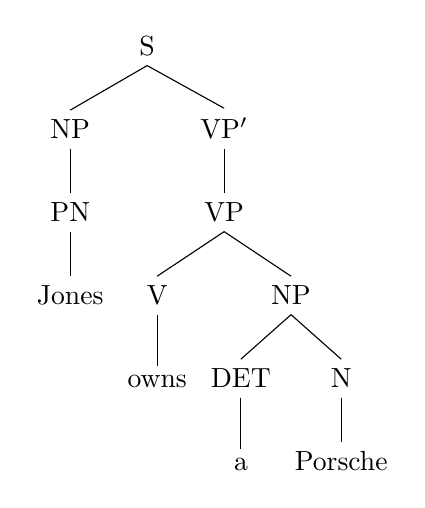
\begin{tikzpicture}
  \Tree [.S [.NP [.PN Jones ] ]
            [.VP$'$ [.VP [.V owns ]
                         [.NP [.DET a ]
                              [.N Porsche ] ] ] ] ]
\end{tikzpicture}
}
& $\to_\crpn$
& \drs{$\drx$}
{
$\obj{Jones}(\drx)$ \\
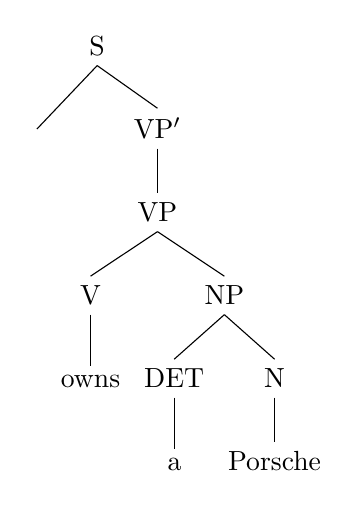
\begin{tikzpicture}
  \Tree [.S $\drx$
            [.VP$'$ [.VP [.V owns ]
                         [.NP [.DET a ]
                              [.N Porsche ] ] ] ] ]
\end{tikzpicture}
}
& $\to_\crid$
& \drs{$\drx$ $\dry$}
{
$\obj{Jones}(\drx)$ \\

\begin{tikzpicture}
  \Tree [.N($\drx$) Porsche ]
\end{tikzpicture} \\
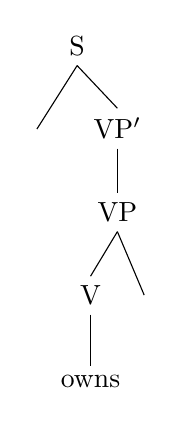
\begin{tikzpicture}
  \Tree [.S $\drx$
            [.VP$'$ [.VP [.V owns ]
                         $\dry$ ] ] ]
\end{tikzpicture}
}
\end{tabular}
\end{center}

We insert the syntactic analysis of the first sentence into the empty
DRS.\@ Then there is a reduction rule which replaces the NP \emph{Jones}
with a discourse referent $\drx$ while at the same time introducing the
discourse referent $\drx$ and the condition $\obj{Jones}(\drx)$ into the DRS.\@
In the next DRS, we evaluate the object by replacing it with $\dry$ and adding
the discourse referent $\dry$ and a condition in which (the meaning of) the
noun \emph{Porsche} is applied to $\dry$.

\begin{center}
\begin{tabular}{rcccccl}
\drs{$\drx$ $\dry$}
{
$\obj{Jones}(\drx)$ \\

\begin{tikzpicture}
  \Tree [.N($\dry$) Porsche ]
\end{tikzpicture} \\
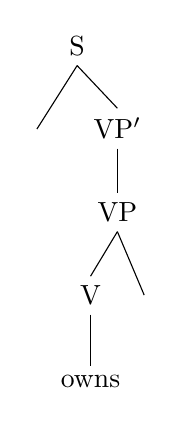
\begin{tikzpicture}
  \Tree [.S $\drx$
            [.VP$'$ [.VP [.V owns ]
                         $\dry$ ] ] ]
\end{tikzpicture}
}
& $\to_\crlin$
& \drs{$\drx$ $\dry$}
{
$\obj{Jones}(\drx)$ \\
$\obj{Porsche}(\dry)$ \\
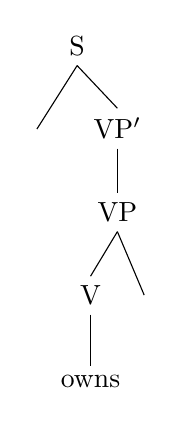
\begin{tikzpicture}
  \Tree [.S $\drx$
            [.VP$'$ [.VP [.V owns ]
                         $\dry$ ] ] ]
\end{tikzpicture}
}
& $=$
& \drs{$\drx$ $\dry$}
{
$\obj{Jones}(\drx)$ \\
$\obj{Porsche}(\dry)$ \\
$[\drx$ owns $\dry]$
}
& $\to_\crlitv$
& \drs{$\drx$ $\dry$}
{
$\obj{Jones}(\drx)$ \\
$\obj{Porsche}(\dry)$ \\
$\obj{own}(\drx, \dry)$
}
\end{tabular}
\end{center}

Having reduced the noun phrase \emph{a Porsche}, we are now led to evaluate
the noun \emph{Porsche} itself. It yields the predicate $\obj{Porsche}$. At
this point, the algorithm presented in~\cite{kamp1993discourse}
stops. However, in order to be a little bit more uniform, we will evaluate
reduce the piece of syntax $[\drx$ owns $\dry]$ and replace it with an
atomic formula $\obj{own}(\drx, \dry)$. We can now add the syntactic
analysis of the second sentence and proceed with computation.


\begin{center}
\begin{tabular}{rcl}
\drs{$\drx$ $\dry$}
{
$\obj{Jones}(\drx)$ \\
$\obj{Porsche}(\dry)$ \\
$\obj{own}(\drx, \dry)$ \\
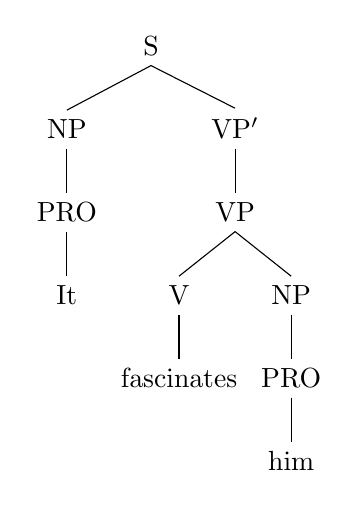
\begin{tikzpicture}
  \Tree [.S [.NP [.PRO It ] ]
            [.VP$'$ [.VP [.V fascinates ]
                         [.NP [.PRO him ] ] ] ] ]
\end{tikzpicture}
}
& $\to_\crpro$
& \drs{$\drx$ $\dry$ $\dru$}
{
$\obj{Jones}(\drx)$ \\
$\obj{Porsche}(\dry)$ \\
$\obj{own}(\drx, \dry)$ \\
$\dru = \dry$ \\
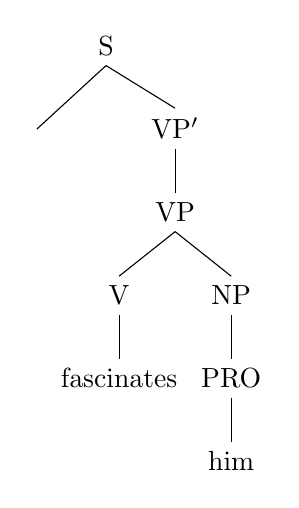
\begin{tikzpicture}
  \Tree [.S $\dru$
            [.VP$'$ [.VP [.V fascinates ]
                         [.NP [.PRO him ] ] ] ] ]
\end{tikzpicture}
}
\end{tabular}
\end{center}

Again, we start by evaluating the subject. This time, it is a pronoun, but
the process remains largely the same. We replace the pronoun with a new
discourse referent $\dru$ which we introduce into the DRS along with the
condition $\dru = \dry$.

\begin{center}
\begin{tabular}{rcccl}
\drs{$\drx$ $\dry$ $\dru$}
{
$\obj{Jones}(\drx)$ \\
$\obj{Porsche}(\dry)$ \\
$\obj{own}(\drx, \dry)$ \\
$\dru = \dry$ \\
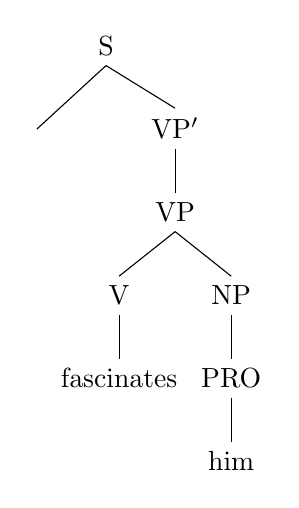
\begin{tikzpicture}
  \Tree [.S $\dru$
            [.VP$'$ [.VP [.V fascinates ]
                         [.NP [.PRO him ] ] ] ] ]
\end{tikzpicture}
}
& $\to_\crpro$
& \drs{$\drx$ $\dry$ $\dru$ $\drv$}
{
$\obj{Jones}(\drx)$ \\
$\obj{Porsche}(\dry)$ \\
$\obj{own}(\drx, \dry)$ \\
$\dru = \dry$ \\
$\drv = \drx$ \\
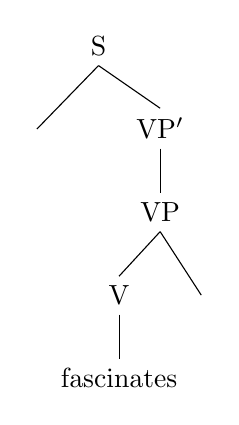
\begin{tikzpicture}
  \Tree [.S $\dru$
            [.VP$'$ [.VP [.V fascinates ]
                         $\drv$ ] ] ]
\end{tikzpicture}
}
& $\to_\crlitv$
& \drs{$\drx$ $\dry$ $\dru$ $\drv$}
{
$\obj{Jones}(\drx)$ \\
$\obj{Porsche}(\dry)$ \\
$\obj{own}(\drx, \dry)$ \\
$\dru = \dry$ \\
$\drv = \drx$ \\
$\obj{fascinate}(\dru, \drv)$
}
\end{tabular}
\end{center}

For the object noun we do the same, introducing the discourse referent
$\drv$ and the condition $\drv = \drx$. Finally, all that is left to
translate the transitive verb into a binary relation and we get the final
DRS representation.

Let us now look at the formulation of the construction rules\footnote{We
  will omit gender features from the rules as we will not be studying
  anaphora resolution in this work.}, starting with $\crid$ in
Figure~\ref{fig:crid}.

\begin{figure}
\centering
\cridbox
\caption{\label{fig:crid} $\crid$: The construction rule for indefinite
  descriptions.}
\end{figure}

The \emph{triggering configuration} describes the rule's redex (and part of
its context). In the case of $\crid$, the rule for indefinite descriptions,
the redex is a noun phrase of the form \emph{a(n) $N$}. The actual
triggering configuration also includes the node dominating the NP as
well. This is for reasons of evaluation order:

\begin{quote}
``A reducible condition $\gamma$ must be reduced by applying the appropriate
rule to its \emph{highest} triggering configuration, i.e.\ that triggering
configuration $\tau$ such that the highest node of $\tau$ dominates the
highest node of any other triggering configuration that $\gamma$ contains.''
\begin{flushright}
  From Discourse to Logic~\cite{kamp1993discourse} (Section 1.1.4, page 87
  in the Student Edition)
\end{flushright}
\end{quote}

In this rule, it serves to make the application of the rule to a subject
dominant to the application of the same rule (or any other rule evaluating,
for that purpose) to an object and therefore fixes evaluation order: first
subject, then object.

The rule then has its contractum, which is given on the last line
(\textbf{Substitute in $\overline{\gamma}$}). In this case, the contractum
is the discourse referent $u$. The rule also has two important side
effects. First, the discourse referent $u$ is introduced into the DRS that
contains this condition. Second, the condition $[N](u)$ is added to the
conditions of that same DRS.\@ The notation $[N](u)$ means that we copy the
whole syntactic structure of $N$ (i.e.\ the whole program for computing the
meaning of the noun) and once its meaning (a predicate) is computed, we
apply it to the discourse referent $u$.

\begin{figure}
\centering
\crprobox
\caption{\label{fig:crpro} $\crpro$: The construction rule for (anaphoric
  third-person singular) pronouns.}
\end{figure}

The rule for pronouns, $\crpro$ in Figure~\ref{fig:crpro}, is very
similar. In introduces a new kind of operation, in which the NP being
evaluated is asking its context for a suitable anaphoric referent.

We will leave the rule for proper nouns until~\ref{sec:presuppositions} and
give the two lexical insertion rules for nouns and transitive verbs
\footnote{the latter is not present in~\cite{kamp1993discourse}. Instead,
  the authors declare [$x$ loves $y$] to be an irreducible condition.}.

\begin{figure}
\begin{subfigure}[b]{0.4\textwidth}
\crlinbox
\caption{\label{fig:crlin} $\crlin$: The lexical insertion rule for
  (common) nouns.}
\end{subfigure}
\hfill
\begin{subfigure}[b]{0.4\textwidth}
\crlitvbox
\caption{\label{fig:crlitv} $\crlitv$: The lexical insertion rule for
  (transitive) verbs.}
\end{subfigure}
\caption{\label{fig:li} The lexical insertion construction rules.}
\end{figure}

The system from~\cite{kamp1993discourse} described above can be presented
in a manner reminiscent of operational semantics for programming languages.

The terms of this language are syntactic trees containing discourse
referents and wrapped inside DRSs. The values are just discourse referents
and DRSs\footnote{Containing only predicates as conditions.}. We will
define evaluation contexts $C$. These should reflect the fact the
construction algorithm of DRT permits reduction in any of the conditions
within a DRS.

$$
  C ::= [] \ | \ \drs{ $\drx_1$ \ldots\ $\drx_n$ }
                { $\gamma_1$ \\ \ldots \\ $\lnot C$ \\ \ldots \\ $\gamma_m$}
           \ | \ \drs{ $\drx_1$ \ldots\ $\drx_n$ }
                { $\gamma_1$ \\ \ldots \\ $C \Rightarrow K$ \\ \ldots \\ $\gamma_m$}
           \ | \ \drs{ $\drx_1$ \ldots\ $\drx_n$ }
                { $\gamma_1$ \\ \ldots \\ $K \Rightarrow C$ \\ \ldots \\ $\gamma_m$}
           \ | \ \drs{ $\drx_1$ \ldots\ $\drx_n$ }
                { $\gamma_1$ \\ \ldots \\ $C \lor K$ \\ \ldots \\ $\gamma_m$}
           \ | \ \drs{ $\drx_1$ \ldots\ $\drx_n$ }
                { $\gamma_1$ \\ \ldots \\ $K \lor C$ \\ \ldots \\ $\gamma_m$}
$$

The reducible conditions are syntactic trees. The triggering configuration
can be found in any part of a syntactic tree and so we define $C_\gamma$ to
be a context that places $[]$ inside a syntactic tree. For every rule
$A \to B_1 \ldots B_n$, there will be a production rule for the context
$C_\gamma ::= A (B_1, \ldots, B_{i-1}, C_\gamma, B_{i+1}, \ldots, B_n)$.

$$
  C_\gamma ::= []\ |\ \leaf{$C_\gamma$} \leaf{VP} \branch{2}{S} \tree
                 \ |\ \leaf{NP} \leaf{$C_\gamma$} \branch{2}{S} \tree
                 \ |\ \leaf{$C_\gamma$} \leaf{NP} \branch{2}{VP} \tree
                 \ |\ \leaf{V} \leaf{$C_\gamma$} \branch{2}{VP} \tree \ |\ \ldots
$$

The construction rule $\crid$ is then a reduction rule on these forms:

$$
  C\left[\ 
    \drs{$\drx_1$ \ldots\ $\drx_n$}
        {$\gamma_1$ \\
         \ldots \\
         $C_\gamma \left[ \leaf{a(n)} \branch{1}{DET} \leaf{N}
           \branch{2}{NP} \leaf{VP$'$} \branch{2}{S} \tree \right]$ \\
         \ldots \\
         $\gamma_m$}\ \right]
  \to_\crid
  C\left[\ 
    \drs{$\drx_1$ \ldots\ $\drx_n$ $\dru$}
        {$\gamma_1$ \\
         \ldots \\
         $[$N$](\dru)$ \\
         $C_\gamma \left[ \leaf{$\dru$} \leaf{VP$'$} \branch{2}{S} \tree \right]$ \\
         \ldots \\
         $\gamma_m$}\ \right]
$$

Likewise, there is an analogue for evaluating indefinite descriptions in
object positions which differs only in the triggerring configuration. The
reduction rules for $\crpro$, $\crlin$ and $\crlitv$ can be derived in the
same way. Then, the DRS that corresponds to a sentence can be seen as a
normal form of in this reduction system\footnote{The system permits
  reductions in different conditions at the same time and is therefore not
  confluent. Hence the indefinite article in ``\emph{a normal form}''.}.

If we look at the rule that we can see a remarkable similarity to the likes
of those seen in Chapter~\ref{chap:continuations} for $\lambda_\shift$ and
$\lambda_\shifto$. Inside the context $C$, we have some kind of delimiting
construction, a DRS in one case and a $\reset$ in the other. As one of the
arguments of this construction, we have an expression buried inside a more
limited context: $C_\gamma$, which cannot contain any more nested DRSs, and
$F$, which cannot contain any more $\reset$s. In the case of DRT, this
buried expression is an indefinite or a pronoun which wants to access the
context's DRS to add (and possibly look for) discourse referents and
conditions. In the case of $\lambda_\shift$, the buried expression is a
$\shift$ that wants complete control over the context inside the
$\reset$. In our analysis of $\lambda_\shift$, $\reset$ corresponded
directly to a handler. Therefore, we will be treating DRSs as handlers in
the coming $\banana{\lambda}$ analysis. The denotations of indefinites and
pronouns will use operations to introduce new discourse referents and
conditions and to query the state of discourse to resolve anaphora.


\section{\texorpdfstring{$\banana{\lambda}$ Analysis}{Analysis in Our Calculus}}
\label{sec:banana-drt}

The first step in building a $\banana{\lambda}$ analysis of dynamics is to
design the effect signature: how many operations we will need, what their
types should be and what they should do. However, our task is largely
facilitated by the fact that in their exposition of
DRT~\cite{kamp1993discourse}, Kamp and Reyle have structured the
construction rules by using a limited set of operations to manipulate the
DRSs. It is these operations that we will include in our effect
signature. Consider the construction rule of pronouns and the corresponding
representation as a $\banana{\lambda}$ computation.

\vspace{6mm}

\hspace{-5mm}
\begin{minipage}{0.63\textwidth}
\crprobox
\end{minipage}
\begin{minipage}{0.36\textwidth}
\vspace{0.4cm}
\begin{align*}
\alpha &: NP \\ \\
\sem{NP} &= \FF_E(\iota)
\end{align*}
\vspace{0.1cm}
\begin{align*}
\sem{\alpha} =\ & \app{\op{choose}}{&&\star}{ &(\lam{v}{ \\
                & \app{\op{introduce}}{&&\star}{ &(\lam{u}{ \\
                & \app{\op{assert}}{&&(u = v)}{ &(\lam{\_}{ \\
                \\ \\
                & \ap{\eta}{u}})}})}})}
\end{align*}
\end{minipage}

\vspace{6mm}

Let $\alpha$ be a third-person singular pronoun\footnote{Since we ignore
  gender, we can think of $\alpha$ as \emph{the} third-person singular
  pronoun}. The construction rule reduces the NP node formed by $\alpha$
into a discourse referent. In the corresponding analysis in our formalism
(ACG + $\banana{\lambda}$), we have $\alpha$ as an abstract constant of
type $NP$ whose semantic interpretation is a computation of type
$\FF_E(\iota)$. The pronoun asks the context for a suitable antecedent,
which is then referred to as $v$. We mimic the verb \textbf{choose} with an
operation $\op{choose}$. It does not take as any inputs, as no inputs are
provided in the construction to the rule\footnote{If we were to care about
  gender markers, the input of this operation would be the gender
  marker/predicate, much like in the example of the $\op{select}$ operator
  proposed in~\ref{ssec:choosing-effect-signature}.}, and expects a
discourse referent in return. Since we will be using the type $\iota$ for
terms that designate individuals, we will identify the type of discourse
referents with $\iota$.

$$
\typedop{choose}{1}{\iota}
$$

Next up, the construction rule demands the introduction of a new discourse
referent into the DRS $\KK$ that contains the condition being
evaluated. This instruction and its use of the verb \textbf{introduce}
gives rise to the $\op{introduce}$ operation. $\op{introduce}$ asks for a
fresh discourse referent and so its type ends being the same as the one for
$\op{choose}$, only the semantics differ\footnote{}:

$$
\typedop{introduce}{1}{\iota}
$$

The next step in the construction rule asks the DRS $\KK$ to introduce a
new condition. For this kind of interaction, \textbf{introducing} a
condition, we will use a new operation, $\op{assert}$. The NP indicates
that the condition it wants to add to the DRS, the truth-condition that it
wants to assert. Conditions are atomic formulas of predicate logic and so
we will use $o$, the type of propositions, to represent them. The output
will be of the trivial type $1$ and we will therefore use the variable name
$\_$, as conventional in functional programming.

$$
\typedop{assert}{o}{1}
$$

Finally, the construction rule tells us to replace the NP node with the
discourse referent $u$. This way, when this NP occurs as an argument to a
predicate, the predicate should be applied to the discourse referent
$u$. In $\banana{\lambda}$, this role is played by the return values of
computations (see equation below). Therefore, we return $u$ with the
computation $\etaE{u}$.

$$
\obj{predicate} \apr (\app{\op{op}}{M_\petitp}{(\lam{x}{ \ldots\
    \etaE{u}})}) = \app{\op{op}}{M_\petitp}{(\lam{x}{ \ldots\
    \etaE{(\obj{predicate}(u))}})}
$$

We can do the same kind of analysis/translation for the $\crid$ rule for
indefinite descriptions.

\vspace{6mm}

\hspace{-10mm}
\begin{minipage}{0.72\textwidth}
\cridbox
\end{minipage}
\begin{minipage}{0.27\textwidth}
\vspace{0.3cm}
\begin{align*}
\abs{a} &: N \limp NP \\
\sem{N} &= \FF_E(\iota \to o) \\
\sem{NP} &= \FF_E(\iota)
\end{align*}
\begin{align*}
\sem{\abs{a}} =\ \lam{N}{& \app{\op{introduce}}{&&\star}{ &(\lam{u}{ \\
                         & N &&\hsbind &(\lam {n}{ \\
                         & \app{\op{assert}}{&&(n(u))}{ &(\lam{\_}{ \\
                         \\
                         & \ap{\eta}{u}})}})})}}
\end{align*}
\end{minipage}

\vspace{6mm}

The $\crid$ rule evaluates a noun phrase which is composed of the
indefinite article followed by some noun $N$. This construction is
represented in our ACG as an abstract constant $\abs{a} : N \limp NP$. Its
denotation will be a function from $\sem{N}$ to $\sem{NP}$. As in the rest
of the analyses seen in this chapter, we will take
$\sem{N} = \FF_E(\iota \to o)$, which meshes with the fact that DRT expects
nouns to reduce to predicates.

The evaluation of the noun phrase ``\emph{a $N$}'' starts by introducing a
fresh discourse referent $u$ and so we use the same operation as in
$\crpro$. Then we will proceed by adding the condition $[N](u)$. Note that
in the DRT rule, we are dealing with a reducible condition ($[N]$ is the
syntax of $N$). In adding this reducible condition, DRT essentially
schedules the evaluation of the syntactic expression $[N]$ via some other
construction rule ($\crlin$ if $N$ is only a common noun, other rules if it
is, e.g., restricted by a relative clause or an adjective). In
$\banana{\lambda}$, we achieve a similar effect by asking for the
evaluation of $N$ using the $\hsbind$ operator. We then state that once the
noun has been evaluated down to a predicate, we want this predicate,
applied to the referent $u$, to be a condition inside the DRS.\@ Finally,
as in $\crpro$, we present the discourse referent $u$ as the referent of
the noun phrase.

For completeness, we will also give translations for the $\crlin$ and
$\crlitv$ rules, even though they do not have any dynamic effects of their
own.

\vspace{6mm}

\begin{minipage}{0.5\textwidth}
\crlinbox
\end{minipage}
\begin{minipage}{0.5\textwidth}
\begin{align*}
\abs{common} &: CN \limp N \\
\sem{CN} &= \iota \to o \\
\sem{N} &= \FF_E(\iota \to o)
\end{align*}
\begin{align*}
\sem{\abs{common}} &= \lam{\alpha}{\etaE{(\lam{v}{\alpha(v)})}} \\
                   &= \lam{\alpha}{\etaE{\alpha}} \\
                   &= \eta
\end{align*}
\end{minipage}

\vspace{6mm}

We, as well as Kamp and Reyle, assume that behind every common noun
$\alpha$ lies a set of individuals, a predicate $\alpha$. The lexical
insertion rule for nouns replaces the noun by that predicate. We can
capture the same line of reasoning in ACGs. We contrast the category $CN$
of common nouns (such as \emph{snowman}, \emph{snake}, \emph{ladder}) to
the larger category $N$ of nouns (\emph{animal in your garden}, \emph{man
  who owns a donkey}). The common nouns will correspond to plain sets of
individuals, $\sem{CN} = \iota \to o$. However, more complex nouns might
also have effects (in the case of dynamics, anaphora, more generally,
deixis, quantification, conventional implicature\ldots) and so we have
$\sem{N} = \FF_E(\iota \to o)$. In ACGs, to say that every common noun $CN$
is a noun $N$ is to provide an injection of type $N \limp
CN$. Homomorphically, its denotation will be an injection from
$\iota \to o$ to $\FF_E(\iota \to o)$, the constructor $\eta$.

\vspace{6mm}

\begin{minipage}{0.5\textwidth}
\crlitvbox
\end{minipage}
\begin{minipage}{0.5\textwidth}
\begin{align*}
\abs{trans} &: V \limp NP \limp NP \limp S \\
\sem{V} &= \iota \to \iota \to o \\
\sem{NP} &= \FF_E(\iota) \\
\sem{S} &= \FF_E(o)
\end{align*}
\begin{align*}
\sem{\abs{trans}} = \lam{\alpha Y X}{&X \hsbind (\lam{x}{ \\
                                     &Y \hsbind (\lam{y}{ \\
                                     &\etaE{(\alpha(x, y))}})})} \\
                  = \lam{\alpha Y X}{&\alpha \apr X \aplr Y}
\end{align*}
\end{minipage}

\vspace{6mm}

With $\crlitv$, the idea behind the DRT/$\banana{\lambda}$ analogy is the
same as with $\crlin$. Behind every (extensional transitive) verb $\alpha$
lies a binary relation, also called $\alpha$. When combined with a subject
and an object, verbs form sentences. This is embodied by the ACG abstract
constant $\abs{trans}$ which maps verbs from $V$ into functions in
$NP \limp NP \limp S$. From the triggerring configuration of the rule
$\crlitv$, we see that (the parent of) the subject dominates (the parent
of) the object. This leads DRT to always evaluate the dynamic effects of
the subject before the object. In $\banana{\lambda}$, this feature is
expressed in the lexical entry for the construction that combines the
subject, verb and object into a sentence, $\abs{trans}$.


\subsection{Example}
\label{ssec:dynamic-example}

We have seen how to map the syntax-semantics construction rules of DRT into
the ACG formalism and how the extra steps performed when reducing
indefinites or pronouns in DRT correspond naturally to operations, with
which we have extended ACG's lambda calculus in $\banana{\lambda}$. We can
now look at an example in action.

\begin{exe}
  \ex \label{ex:man-porsche} A man owns a Porsche. It fascinates him.
\end{exe}

This is a small variation of Example~\ref{ex:jones-porsche} in which
\emph{Jones} was replaced by \emph{a man}\footnote{We relegate the
  discussion of proper nouns to~\ref{sec:presuppositions}.}.

\begin{align*}
  \sem{\appp{\abs{trans}}{&\abs{owns}}{(\ap{\abs{a}}{(\ap{\abs{common}}{\abs{Porsche}})})}{(\ap{\abs{a}}{(\ap{\abs{common}}{\abs{man}})})}} \\
  \tto &\ \app{\op{introduce}}{\star}{(\lam{x}{ \\
       &\ \app{\op{assert}}{(\obj{man}(x))}{(\lam{\_}{ \\
       &\ \app{\op{introduce}}{\star}{(\lam{y}{ \\
       &\ \app{\op{assert}}{(\obj{Porsche}(y))}{(\lam{\_}{ \\
       &\ \etaE{(\obj{own}(x, y))}})}})}})}})}
\end{align*}

The only effects are due to the indefinites that introduce new discourse
referents and assert truth conditions. The operations are ordered
subject-first, object-last and the computation returns the predicate that
is the application of the verb's predicate to the referents of the subject
and the object. The same goes for the second sentence in
Example~\ref{ex:man-porsche}:

\begin{align*}
  \sem{\appp{\abs{trans}}{&\abs{fascinates}}{\abs{him}}{\abs{it}}} \\
  \tto &\ \app{\op{choose}}{\star}{(\lam{y'}{ \\
       &\ \app{\op{introduce}}{\star}{(\lam{u}{ \\
       &\ \app{\op{assert}}{(u = y')}{(\lam{\_}{ \\
       &\ \app{\op{choose}}{\star}{(\lam{x'}{ \\
       &\ \app{\op{introduce}}{\star}{(\lam{v}{ \\
       &\ \app{\op{assert}}{(v = x')}{(\lam{\_}{ \\
       &\ \etaE{(\obj{fascinate}(u, v))}})}})}})}})}})}})}
\end{align*}

We can compose the two using $\andlr$, the conjunction of propositions
raised to computations.

\begin{align*}
  \sem{\appp{\abs{trans}}{&\abs{owns}}{(\ap{\abs{a}}{(\ap{\abs{common}}{\abs{Porsche}})})}{(\ap{\abs{a}}{(\ap{\abs{common}}{\abs{man}})})}} \andlr \sem{\appp{\abs{trans}}{\abs{fascinates}}{\abs{him}}{\abs{it}}} \\
  \tto &\ \app{\op{introduce}}{\star}{(\lam{x}{ \\
       &\ \app{\op{assert}}{(\obj{man}(x))}{(\lam{\_}{ \\
       &\ \app{\op{introduce}}{\star}{(\lam{y}{ \\
       &\ \app{\op{assert}}{(\obj{Porsche}(y))}{(\lam{\_}{ \\
       &\ \app{\op{choose}}{\star}{(\lam{y'}{ \\
       &\ \app{\op{introduce}}{\star}{(\lam{u}{ \\
       &\ \app{\op{assert}}{(u = y')}{(\lam{\_}{ \\
       &\ \app{\op{choose}}{\star}{(\lam{x'}{ \\
       &\ \app{\op{introduce}}{\star}{(\lam{v}{ \\
       &\ \app{\op{assert}}{(v = x')}{(\lam{\_}{ \\
       &\ \etaE{(\obj{own}(x, y) \land \obj{fascinate}(u, v))}})}})}})}})}})}})}})}})}})}})}
\end{align*}

The resulting computation introduces 4 discourse referents: $x$, $y$, $u$
and $v$. Assuming that $\op{choose}$ will give us $x$ for $x'$ and $y$ for
$y'$, then we end up introducing and returning the conditions
$\obj{man}(x)$, $\obj{Porsche}(y)$, $u = x$, $v = y$, $\obj{own}(x, y)$ and
$\obj{fascinate}(u, v)$, i.e.\ the same conditions as in the DRS for
Example~\ref{ex:jones-porsche} (replacing $\obj{Jones}(x)$ with
$\obj{man}(x)$). However, while that might be our desired interpretation of
this computation, for now, it is just a string of symbols.


\subsection{Handler for Dynamics}
\label{ssec:handler-for-dynamics}

In order to give a formal semantics to the operations that we have
introduced for DRT, we will write a handler. The type of dynamic
propositions, $\gamma \to (\gamma \to o) \to o$, of de Groote's TTDL will
serve as a suitable interpretation domain. On top of that, apart from
implementing a semantics for our operations, we will have demonstrated the
link between DRT and TTDL.\@ The type of the handler's input will be
$\FF_E(o)$, where $E$ is the effect signature containing only
$\op{choose}$, $\op{introduce}$ and $\op{assert}$.

\begin{align*}
  \TTDL :\ &\FF_E(o) \to \gamma \to (\gamma \to o) \to o \\
  \TTDL = \bbanana{\ 
  &\onto{\op{choose}}{(\lam{\_ k e \phi}{\appp{k}{(\sel(e))}{e}{\phi}})}, \\
  &\onto{\op{introduce}}{(\lam{\_ k e \phi}{\exists x.\ \appp{k}{x}{(x \cons e)}{\phi}})}, \\
  &\onto{\op{assert}}{(\lam{p k e \phi}{p \land \appp{k}{\star}{(p \cons e)}{\phi}})}, \\
  &\onto{\eta}{(\lam{p e \phi}{p \land \ap{\phi}{e}})}\ }
\end{align*}

We write the handler by following the types, keeping in mind the intended
semantics. There is a remarkable similarity between the clauses of our
handler and the operators and semantic entries used in TTDL.\@ The $\eta$
clause is the operation that lifts plain propositions into dynamic
propositions~\cite{lebedeva2012expression}. The clause for $\op{choose}$ is
(ignoring the first dummy argument) exactly the denotation assigned to
pronouns in TTDL~\cite{de2006towards}. The clause for $\op{introduce}$ is
the denotation of the indefinite \emph{someone}, also known as the dynamic
existential quantifier in~\cite{lebedeva2012expression}. This is not a
coincidence. The clauses for $\op{choose}$ and $\op{introduce}$ are both
values of type $\iota$ written in continuation-passing style with
observation type $\Omega = \gamma \to (\gamma \to o) \to o$, i.e.\ values
of type $(\iota \to \Omega) \to \Omega$. TTDL uses continuation-passing
style in the denotation of its noun phrases to account for quantification
and so their denotations end up having the very same type. The two noun
phrases, the pronoun and the indefinite, stand for the two major ways that
dynamic noun phrases interact with their contexts, retrieving their
referents from context or introducing new ones into the context. Together
with $\op{assert}$, which lets us conjoin another proposition to the
observed proposition, these form the three operations with which we
characterize DRT dynamics. Our original discovery of these three operations
with which we can characterize dynamic effects came from the realization
that we can express all the denotations in TTDL with: reading from the
context ($\op{choose}$, or later $\op{get}$), wrapping an existential
quantifier over the continuation while adding the bound variable into the
context ($\op{introduce}$) and conjoining a proposition to the continuation
($\op{assert}$).

Once we have applied the $\TTDL$ handler to a computation of type
$\FF_E(o)$, we can extract the corresponding (simple) proposition by
applying the result to some left context and the trivial right context
($\lam{e}{\top}$). Since this what we will be doing most of the time, we
can simplify the $\TTDL$ handler by assuming that $\phi$ is always equal to
$\lam{e}{\top}$.

\begin{align*}
  \BOX :\ &\FF_E(o) \to \gamma \to o \\
  \BOX = \bbanana{\ 
  &\onto{\op{choose}}{(\lam{\_ k e}{\app{k}{(\sel(e))}{e}})}, \\
  &\onto{\op{introduce}}{(\lam{\_ k e}{\exists x.\ \app{k}{x}{(x \cons e)}})}, \\
  &\onto{\op{assert}}{(\lam{p k e}{p \land \app{k}{\star}{(p \cons e)}})}, \\
  &\onto{\eta}{(\lam{p e}{p})}\ }
\end{align*}

The handler is called $\BOX$ to stress the analogy to DRSs, which are
customarily drawn as boxes. The crucial common point is that putting
something in a box means that any truth conditions or discourse referents
that it introduces are contained within the box. Throughout this chapter,
we will refer to applications of this handler as boxes, DRSs or
contexts\footnote{Since the handler acts as something that provides and
  regulates access to a (left) TTDL context.}.

Getting back to Example~\ref{ex:man-porsche}, we can now apply one of these
two handlers to get the dynamic proposition.

\begin{align*}
&\ap{\TTDL}{(\sem{\appp{\abs{trans}}{\abs{owns}}{(\ap{\abs{a}}{(\ap{\abs{common}}{\abs{Porsche}})})}{(\ap{\abs{a}}{(\ap{\abs{common}}{\abs{man}})})}} \andlr \sem{\appp{\abs{trans}}{\abs{fascinates}}{\abs{him}}{\abs{it}}})} \\
&\tto \lam{e \phi}{\exists x.\ \obj{man}(x) \land (\exists y.\ \obj{Porsche}(y) \land (\exists u.\ u = \sel(e_1) \land (\exists v.\ v = \sel(e_2) \land \obj{own}(x, y) \land \obj{fascinate}(u, v) \land \ap{\phi}{e_3})))} \\
&= \lam{e \phi}{\exists x y u v.\ \obj{man}(x) \land \obj{Porsche}(y) \land u = \sel(e_1) \land v = \sel(e_2) \land \obj{own}(x, y) \land \obj{fascinate}(u, v) \land \ap{\phi}{e_3}} \\
&= \lam{e \phi}{\exists x y u v.\ \obj{man}(x) \land \obj{Porsche}(y) \land u = y \land v = x \land \obj{own}(x, y) \land \obj{fascinate}(u, v) \land \ap{\phi}{e_3}} \\
&= \lam{e \phi}{\exists x y.\ \obj{man}(x) \land \obj{Porsche}(y) \land \obj{own}(x, y) \land \obj{fascinate}(y, x) \land \ap{\phi}{e_3}}
\end{align*}

where:
\vspace{-1mm}
\begin{align*}
  e_1 &= \obj{Porsche}(y) \cons y \cons \obj{man}(x) \cons x \cons e \\
  e_2 &= (u = \sel(e_1)) \cons u \cons e_1 \\
  e_3 &= (v = \sel(e_2)) \cons v \cons e_2
\end{align*}

We have used Kamp's construction rules to compute a dynamic proposition in
de Groote's TTDL.\@ The first line shows the result as we get it from the
handler. On the second line, we pull out all of the existential quantifiers
(prenex form). On the third line, we resolve the anaphora and we get a
dynamic proposition which corresponds referent by referent, condition by
condition to the DRS derived by Kamp and Reyle. The last line removes
spurious variables and equalities.


\subsection{Negation}
\label{ssec:dynamic-negation}

In order to match the empirical coverage of the original TTDL
from~\cite{de2006towards}, we have two more features to cover: negation and
(universal) quantification. We will cover negation here. Quantification
reuses the idea from negation and the $\op{scope}$ operation of
quantification: we will see how the two connect in
Chapter~\ref{chap:composing-effects}.

\begin{figure}
  \centering
  \crnegbox
  \caption{\label{fig:crneg} $\crneg$: The construction rule for negation.}
\end{figure}

The construction rule for negation, $\crneg$, is displayed in
Figure~\ref{fig:crneg}. We are reducing a condition which is in the form of
a negated sentence. The DRT mechanism will place the sentence in its own
DRS, whose negation will then become the new condition that replaces the
sentence. The dynamic effects that we have seen so far reach only into the
nearest enclosing DRS.\@ This means that wrapping something inside a new
DRS is significant: the reach of any dynamic effects within will be limited
to that DRS.\@ We have also seen that this is akin to the way effects like
$\shift$ are delimited/handled by the nearest $\reset$. It will come as no
surprise then that our implementation of negation will use a handler for
dynamic effects.

The definition of dynamic negation in TTDL
from~\cite{lebedeva2012expression} will be a great guide in how to proceed:

\begin{align*}
\dnot_{\TTDL} \_ &: \Omega \to \Omega \\
\dnot_{\TTDL} A &= \lam{e \phi}{\lnot (\app{A}{e}{(\lam{e}{\top})}) \land \ap{\phi}{e}}
\end{align*}

We know that $\lam{e \phi}{M \land \ap{\phi}{e}}$ corresponds to $\etaE{M}$
and that $\app{A}{e}{(\lam{e}{\top})}$ is $\app{\BOX}{A}{e}$. Therefore, we
can define our dynamic negation by:

\begin{align*}
\dnot \_ &: \FF_E(o) \to \FF_E(o) \\
\dnot A &= \etaE{(\lnot (\app{\BOX}{A}{e}))}
\end{align*}

However, there is a small catch. We have a free variable $e$ of type
$\gamma$. This is supposed to be the context in which the new negated
condition is to appear. This is necessary so that the anaphoric elements
within the negated condition can refer to not only referents proper to the
negated DRS, but also those originating in superordinate DRSs. We can
introduce a new operation for accessing the context.

$$
\typedop{get}{1}{\gamma}
$$

Now, we can have dynamic negation as:

$$
\dnot A = \app{\op{get}}{\star}{(\lam{e}{\etaE{(\lnot (\app{\BOX}{A}{e}))}})}
$$

We can see the analogy with $\crneg$: the negation of $A$ puts $A$ inside a
box, the box is then negated and returned as the new condition. The name
$\BOX$ for this kind of handler was motivated exactly by this kind of
analogy, wherein a handler is used to contain dynamic effects inside some
scope.

We have introduced a new operation into our dynamic effect signature. This
means that we will have to extend our handlers to cover the new
operation. However, before we do so, we note that $\op{choose}$ can be
expressed in terms of $\op{get}$ and $\sel$:

$$
\op{choose} = \lam{\_ k}{\app{\op{get}}{\star}{(\lam{e}{\ap{k}{(\sel(e))}})}}
$$

Therefore, we will drop $\op{choose}$ and keep only $\op{get}$. We have now
arrived at our final effect signature for DRT dynamics. This signature
allows us to treat dynamic effects the same way as the other effects that
we have analyzed in this chapter.

\begin{align*}
  E_\DRT = \{\ &\typedop{get}{1}{\gamma}, \\
              &\typedop{introduce}{1}{\iota}, \\
              &\typedop{assert}{o}{1}\ \}
\end{align*}

The closed handlers $\TTDL$ and $\BOX$ are updated to use $\op{get}$
instead of $\op{choose}$:

\begin{align*}
  \TTDL :\ &\FF_{E_\DRT}(o) \to \gamma \to (\gamma \to o) \to o \\
  \TTDL = \bbanana{\ 
  &\onto{\op{get}}{(\lam{\_ k e \phi}{\appp{k}{e}{e}{\phi}})}, \\
  &\onto{\op{introduce}}{(\lam{\_ k e \phi}{\exists x.\ \appp{k}{x}{(x \cons e)}{\phi}})}, \\
  &\onto{\op{assert}}{(\lam{p k e \phi}{p \land \appp{k}{\star}{(p \cons e)}{\phi}})}, \\
  &\onto{\eta}{(\lam{p e \phi}{p \land \ap{\phi}{e}})}\ } \\ \\
  \BOX :\ &\FF_{E_\DRT}(o) \to \gamma \to o \\
  \BOX = \bbanana{\ 
  &\onto{\op{get}}{(\lam{\_ k e}{\app{k}{e}{e}})}, \\
  &\onto{\op{introduce}}{(\lam{\_ k e}{\exists x.\ \app{k}{x}{(x \cons e)}})}, \\
  &\onto{\op{assert}}{(\lam{p k e}{p \land \app{k}{\star}{(p \cons e)}})}, \\
  &\onto{\eta}{(\lam{p e}{p})}\ }
\end{align*}


\subsection{Truth Conditions as Side Effects}
\label{ssec:truth-conditions-side-effects}

Let us look back the computation that we assigned to the first sentence in
Example~\ref{ex:man-porsche}: \emph{a man owns a Porsche}.

\begin{align*}
&\app{\op{introduce}}{\star}{(\lam{x}{ \\
&\app{\op{assert}}{(\obj{man}(x))}{(\lam{\_}{ \\
&\app{\op{introduce}}{\star}{(\lam{y}{ \\
&\app{\op{assert}}{(\obj{Porsche}(y))}{(\lam{\_}{ \\
&\etaE{(\obj{own}(x, y))}})}})}})}})}
\end{align*}

The truth condition that corresponds to the verb is being returned by the
computation, whereas the truth conditions that arise from the nouns are
expressed using $\op{assert}$. The at-issue content of this sentence
consists of all of these conditions and therefore there is no reason to
separate out the verb's predicate. We could thus write this instead:

\begin{align*}
&\app{\op{introduce}}{\star}{(\lam{x}{ \\
&\app{\op{assert}}{(\obj{man}(x))}{(\lam{\_}{ \\
&\app{\op{introduce}}{\star}{(\lam{y}{ \\
&\app{\op{assert}}{(\obj{Porsche}(y))}{(\lam{\_}{ \\
&\app{\op{assert}}{(\obj{own}(x, y))}{(\lam{\_}{ \\
&\etaE{\star}})}})}})}})}})}
\end{align*}

This is a computation of type $\FF_{E_\DRT}(1)$. As before, we use a
handler to extract the proposition that is represented by this computation.

\begin{align*}
  \TTDL :\ &\FF_{E_\DRT}(1) \to \gamma \to (\gamma \to o) \to o \\
  \TTDL = \bbanana{\ 
  &\onto{\op{choose}}{(\lam{\_ k e \phi}{\appp{k}{(\ap{\sel}{e})}{e}{\phi}})}, \\
  &\onto{\op{introduce}}{(\lam{\_ k e \phi}{\exists x.\ \appp{k}{x}{(x \cons e)}{\phi}})}, \\
  &\onto{\op{assert}}{(\lam{p k e \phi}{p \land \appp{k}{\star}{(p \cons e)}{\phi}})}, \\
  &\onto{\eta}{(\lam{\_ e \phi}{\ap{\phi}{e}})}\ }
\end{align*}

The handler differs from the original $\TTDL$ only in the $\eta$ clause,
which substitutes $\top$ for the returned proposition $p$ in
$\lam{e \phi}{p \land \ap{\phi}{e}}$.

We can use computations of type $\FF_{E_\DRT}(1)$ as our type of dynamic
(i.e.\ effectful) propositions. We can embed simple propositions using
$\op{assert}!$, which has type $o \to \FF_{E_\DRT}(1)$. We can perform
dynamic conjunction $M \dand N$ by chaining two computations,
$M \hsbind (\lam{\_}{N}) : \FF_{E_\DRT}(1)$ for $M, N :
\FF_{E_\DRT}(1)$. We can modify $\BOX$ the same way we modified
$\TTDL$. Dynamic negation will be the same as before, with $\eta$ being
replaced with $\op{assert}!$.

\begin{align*}
  \BOX :\ &\FF_{E_\DRT}(1) \to \gamma \to o \\
  \BOX = \bbanana{\ 
  &\onto{\op{get}}{(\lam{\_ k e}{\app{k}{e}{e}})}, \\
  &\onto{\op{introduce}}{(\lam{\_ k e}{\exists x.\ \app{k}{x}{(x \cons e)}})}, \\
  &\onto{\op{assert}}{(\lam{p k e}{p \land \app{k}{\star}{(p \cons e)}})}, \\
  &\onto{\eta}{(\lam{\_ e}{\top})}\ }
\end{align*}

$$
\dnot A = \app{\op{get}}{\star}{(\lam{e}{\ap{\op{assert}!}{(\lnot (\app{\BOX}{A}{e}))}})}
$$

In the lexical entries derived from the construction rules, not much will
have to change. We will only see a difference in the lexical entry
$\abs{trans}$ that we have introduced for the $\crlitv$ rule for transitive
verbs (which was extrapolated from the DRT treatment
in~\cite{kamp1993discourse}). Instead of returning the proposition as the
result of evaluating the sentence, we add it as a condition using
$\op{assert}!$, which is actually what the DRS construction algorithm ends
up doing.

\begin{align*}
\abs{trans} &: V \limp NP \limp NP \limp S \\
\sem{\abs{trans}} &= \lam{\alpha Y X}{(\alpha \apr X \aplr Y) \hsbind \op{assert}!}
\end{align*}

This means that we can build up our dynamic semantics using computations
that do not return anything, only modify the context using side
effects. This is very much in the spirit of dynamic semantics: meaning is
context change potential~\cite{sep-dynamic-semantics}.

If we look closer at TTDL, we can see that the same strategy is applied
there. Let $S$ be the state monad which maps the type $\alpha$ to the type
$\gamma \to (\alpha \times \gamma)$. This is the monad that underlies
state, such as the storing and retrieving of discourse referents. Its
corresponding monad transformer $S(F)$ maps the type $\alpha$ to the type
$\gamma \to F(\alpha \times \gamma)$. Let $C$ be the continuation monad
which maps the type $\alpha$ to the type $(\alpha \to o) \to o$. By
applying the $S$ monad transformer to the $C$ monad, we get a monad $S(C)$
that maps the type $\alpha$ to the type
$\gamma \to (\alpha \times \gamma \to o) \to o$. This monad characterizes
computations that have read/write access to some state of type $\gamma$ and
can manipulate their continuation of type $o$. If we look at such
computations of return type $1$, we get a computation type
$\gamma \to (1 \times \gamma \to o) \to o$. By the isomorphism between
$1 \times \gamma$ and $\gamma$, this is the same as
$\gamma \to (\gamma \to o) \to o$, which is the type $\Omega$ of dynamic
propositions in TTDL.\@ The correspondence is not a shallow coincidence of
types, but many of the terms of TTDL can be generated using the $\eta$ and
$\hsbind$ of this monad.

The switch from $\FF_E(o)$ to $\FF_{E \uplus DRT}(1)$ is very much like the
one from $\FF_E((\iota \to o) \to o)$ to
$\FF_{E \uplus \op{scope}}(\iota)$: we found a way to encode
quantifiers/truth conditions as side effects and so we move the extra
structure from the return type to the effect signature. The choice between
the two is rather arbitrary. Keeping $o$ as the return type for
computations that interpret sentences is more consistent with what we have
been doing in Chapter~\ref{chap:introducing-effects}. On the other hand,
using $1$ as the return type:

\begin{itemize}
\item is more uniform by not admitting both $\etaE{A}$ and
  $\ap{\op{assert}!}{A}$
\item which leads to nicer canonical representations and equational theory
  in~\ref{ssec:algebraic-drt}
\item in order to correctly treat the cancellation of presuppositions
  in~\ref{sec:presuppositions}, we will need to add the truth-conditions
  generated by verbs into the context using something like $\op{assert}$
  anyway
\end{itemize}

For the remainder of this chapter, we will use the encoding that models
sentences as computations of return type $1$.


\subsection{Algebraic Considerations}
\label{ssec:algebraic-drt}

Now that we have handlers for our computations, we can study which
computations share the same interpretations and try to derive some
equational theory over them.

We will first start by looking at how $\op{get}$ behaves w.r.t.\ itself and
the other operations.

\begin{align*}
   \app{\op{get}}{\star}{(\lam{e}{\app{\op{get}}{\star}{(\lam{e'}{M(e, e')})}})}
&= \app{\op{get}}{\star}{(\lam{e}{M(e, e)})} \\
   M
&= \app{\op{get}}{\star}{(\lam{e}{M})}
\end{align*}

As with the $\op{speaker}$ getter from~\ref{sec:deixis}, we get two laws
telling us that asking for the context is idempotent (first equation) and
that it has no other bearing on the result of the computation (second
equation).

Since we know how $\op{assert}$ and $\op{introduce}$ modify the context, we
can reorder $\op{get}$ w.r.t.\ these two operations:

\begin{align*}
   \app{\op{assert}}{A}{(\lam{u}{\app{\op{get}}{\star}{(\lam{e}{M(u, e)})}})}
&= \app{\op{get}}{\star}{(\lam{e}{\app{\op{assert}}{A}{(\lam{u}{M(u, A \cons e)})}})} \\
   \app{\op{introduce}}{\star}{(\lam{x}{\app{\op{get}}{\star}{(\lam{e}{M(x, e)})}})}
&= \app{\op{get}}{\star}{(\lam{e}{\app{\op{introduce}}{\star}{(\lam{x}{M(x, x \cons e)})}})} \\
\end{align*}

This means we can assume that every computation of type $\FF_{E_\DRT}(1)$
uses $\op{get}$ exactly once and does so at the very beginning, i.e.\ it is
of the form $\app{\op{get}}{\star}{(\lam{e}{M(e)})}$ where
$M(e) : \FF_{\{\op{implicate}, \op{assert}\}}(1)$\footnote{When writing
  effect signatures in subscripts, we will often omit the types of
  operations, which are presumed to be constant.}.

If we assume that relative order of discourse referents and conditions is
not important (i.e.\ they are both separate parts, as in a DRS),
$x \cons p \cons e = p \cons x \cons e$ for $x : \iota$, $p : o$ and
$e : \gamma$, then we get the following equation:

$$
  \app{\op{assert}}{A}{(\lam{u}{\app{\op{introduce}}{\star}{(\lam{x}{M(u, x)})}})} 
= \app{\op{introduce}}{\star}{(\lam{x}{\app{\op{assert}}{A}{(\lam{u}{M(u, x)})}})}
$$

This will allows us to move $\op{introduce}$ operations above $\op{assert}$
operations so that we can have the following canonical representation for
computations of type $\FF_{E_\DRT}(1)$:

\begin{align*}
  &\app{\op{get}}{\star}{(\lam{e}{ \\
  &\app{\op{introduce}}{\star}{(\lam{x_1}{ \\
  &\qquad \cdots \\
  &\app{\op{introduce}}{\star}{(\lam{x_n}{ \\
  &\app{\op{assert}}{c_1}{(\lam{\_}{ \\
  &\qquad \cdots \\
  &\app{\op{assert}}{c_m}{(\lam{\_}{ \\
  &\etaE{\star}})}})}})}})}})}
\end{align*}

In other words, the computation examines its context $e$ and then produces
the DRS:

\vspace{2mm}

\drs{$x_1$\ \ldots\ $x_n$}{$c_1$ \\ $\cdots$ \\ $c_m$}

\vspace{2mm}

Note that as in TTDL, discourse referents correspond to $\lambda$-binders
in $\banana{\lambda}$ and their standard notion of $\alpha$-equivalence
gives rise to $\alpha$-equivalence for our representations.

If we were to further assume that the order in contexts does not matter at
all (i.e.\ the discourse referents and conditions form sets, as in a DRS),
$x \cons y \cons e = y \cons x \cons e$ and
$p \cons q \cons e = q \cons p \cons e$ for $x, y : \iota$, $p, q : o$ and
$e : \gamma$, then we get the following:

\begin{align*}
   \app{\op{assert}}{A}{(\lam{u_1}{\app{\op{assert}}{B}{(\lam{u_2}{M(u_1, u_2)})}})} 
&= \app{\op{assert}}{B}{(\lam{u_2}{\app{\op{assert}}{A}{(\lam{u_1}{M(u_1, u_2)})}})} \\
   \app{\op{introduce}}{\star}{(\lam{x}{\app{\op{introduce}}{\star}{(\lam{y}{M(x, y)})}})} 
&= \app{\op{introduce}}{\star}{(\lam{y}{\app{\op{introduce}}{\star}{(\lam{x}{M(x, y)})}})}
\end{align*}

Since the discourse referents and conditions are (unordered) sets in the
presentation in~\cite{kamp1993discourse}, this would make our
representation closer to DRSs.

Finally, if we assume that the conditions in a context can be seen as a big
conjunction, $p \cons q \cons e = (p \land q) \cons e$ for $p, q : o$ and
$e : \gamma$, then we admit the following equations:

$$
  \app{\op{assert}}{A}{(\lam{u}{\app{\op{assert}}{B}{(\lam{u'}{M(u, u')})}})} 
= \app{\op{assert}}{(A \land B)}{(\lam{u}{M(u, u)})}
$$

which gives us a simpler canonical representation:

\begin{align*}
  &\app{\op{get}}{\star}{(\lam{e}{ \\
  &\app{\op{introduce}}{\star}{(\lam{x_1}{ \\
  &\qquad \cdots \\
  &\app{\op{introduce}}{\star}{(\lam{x_n}{ \\
  &\app{\op{assert}}{p}{(\lam{\_}{ \\
  &\etaE{\star}})}})}})}})}
\end{align*}

This boils down a computation of type $\FF_{E_\DRT}(1)$ into a proposition
$p$ that depends on some context $e$ and introduces the new discourse
referents $x_1$, \ldots, $x_n$.


\section{Presuppositions}
\label{sec:presuppositions}

In our $\banana{\lambda}$ analysis of anaphora, we have completely omitted
proper nouns, even though they are treated by DRT
in~\cite{kamp1993discourse} and feature in
Example~\ref{ex:jones-porsche}. This is due to the fact that proper nouns
trigger presuppositions: \emph{Jones sleeps} presupposes that there is some
(contextually salient) entity named Jones. These presuppositions project
outside of entailment-cancelling operators such as negation, outside of the
DRSs in which they are contained.

\begin{exe}
  \ex \label{ex:jones-mercedes} It is not the case that Jones owns a
  Porsche. He owns a Mercedes.
\end{exe}

In Example~\ref{ex:jones-mercedes}, the proper noun \emph{Jones}
contributes a discourse referent which is then picked up in the second
sentence. This would be impossible to achieve using $\op{introduce}$, since
that would contribute the referent only to the DRS ($\BOX$) that is being
negated and the discourse referent would not reach the second sentence.

\begin{figure}
\centering
\crpnbox
\caption{\label{fig:crpn} $\crpn$: The construction rule for proper nouns.}
\end{figure}

If we look at the construction rule for proper nouns in DRT, $\crpn$,
displayed on Figure~\ref{fig:crpn}, we will see that the discourse referent
and the condition describing it are being inserted into the main DRS and
not into the DRS $K$, in which the condition being reduced appears.

In TTDL, this issue was resolved by adding exceptions into the lambda
calculus used for the semantic terms~\cite{lebedeva2012expression}. The
lexical entry for a presupposition trigger such as a proper noun or a
definite description throws an exception,
$(\texttt{AbsentIndividualExc}\ P)$. This exception carries the predicate
$P$ that describes the entity that is presupposed to exist. At the top
level, a handler catches these exceptions and accommodates these
presuppositions. We have seen that in $\banana{\lambda}$, dynamic
propositions are modelled as computations and these computations already
have a notion of throwing exceptions (effects) and handling them
(handlers). We will introduce an operation named $\op{presuppose}$. Its
input type will be $\iota \to o$, a predicate that describes the entity
whose existence is presupposed. The output type will be $\iota$, the
presupposed entity satisfying the predicate.

$$
\typedop{presuppose}{(\iota \to o)}{\iota}
$$

The type of this operation is not exactly equivalent to the exception
$\texttt{AbsentIndividualExc}$ from~\cite{lebedeva2012expression}. As we
have seen in Chapter~\ref{ssec:expressions-as-computations}, exceptions are
effects that have the impossible output type $0$, which means that no
handler will be able to resume the computation by using the
continuation. In Lebedeva's approach, when the toplevel handler intercepts
the exception, it accommodates the presupposition, rewinds the dynamic
state and evaluates the sentence again, this time with a context which now
contains the presupposed entity. This is not suitable to our approach
because of two reasons:

\begin{itemize}
\item We will deal with many other effects besides dynamic state and
  rewinding all of their effects in order to evaluate the sentence again in
  a new context would be needlessly complex.
\item This approach over-generates by licencing the reading ``He$_1$ loves
  John's$_1$ car''. When evaluating \emph{John}, the existence of John is
  presupposed and the sentence is evaluated again, in a context in which
  John is accessible. However, this will allow the pronoun in subject
  position to resolve to John and end up being bound by the object.
\end{itemize}

The effects in $\banana{\lambda}$ differ from traditional exceptions in
that they are resumable. Besides having the input type (which is the
message type of a traditional exception), they also have an output
type. Handlers can then resume computation at the point of the effect by
calling the continuation with a value of the output type. We make full use
of this in our treatment of presuppositions by using $\iota$ as the output
type of $\op{presuppose}$. This way, we do not have to abort the evaluation
of the sentence, rewind all of the effects and evaluate it again; we return
the presupposed entity immediately and the evaluation of the sentence
continues. This strategy also avoid the over-generation mentioned above, in
which a presupposition trigger binds a pronoun preceding it.

We have shown have the $\op{presuppose}$ operation can be motivated on the
grounds of the analysis done by Lebedeva
in~\cite{lebedeva2012expression}. We can also look at how it ties to the
DRT construction rule for presupposition triggers such as $\crpn$. When
translating construction rules into computations, we have implemented the
\textbf{Introduce in $\universe_K$} command as the $\op{introduce}$
operation and the \textbf{Introduce in $\conditions_K$} as the
$\op{assert}$ operation. We might therefore proceed the same way and
translate the \textbf{Introduce into the universe of the main DRS} command
as some operation $\typedop{introduce\_main}{\star}{\iota}$ and
\textbf{Introduce into the condition set of the main DRS} command as
$\typedop{assert\_main}{o}{1}$. However, by looking at the construction
rules of presupposition triggers, we see that they tend to use the two
operations in tandem: first introduce a new discourse referent and then
some condition(s) describing it. Therefore, we can fuse the two into a
single operation $\typedop{presuppose}{(\iota \to o)}{\iota}$, which
introduces and outputs a new discourse referent $x$ while at the same it
introduces the condition $P(x)$, where $P$ is its argument.

Besides lowering the number of basic operations that we have to introduce,
this also has an advantage when we start to consider ambiguous ways of
accommodating presuppositions
(\ref{ssec:presupposition-ambiguities}). Suppose we have two operations,
$\op{introduce\_somewhere}$ and $\op{assert\_somewhere}$, that let us
introduce discourse referents and conditions into arbitrary DRSs on the
projection line\footnote{A \emph{projection line} is a path in the
  accessibility tree from a sub-DRS to the root of the
  tree~\cite{van1992presupposition}.}. We might then end up accommodating
the discourse referent and the condition in different DRS, yielding an
undesired meaning. If we package the two operations into a single
$\op{presuppose\_somewhere}$, then we do not have this problem.


\subsection{Revising the Dynamic Handler}
\label{ssec:revising-dynamic-handler}

We will want to introduce the $\op{presuppose}$ operation into our dynamic
semantics in such a way that $\op{presuppose}$ projects outside of boxes
(DRSs, applications of the $\BOX$ handler). This means that applying the
$\BOX$ handler to a computation should yield a computation free of
$\op{get}$, $\op{introduce}$ and $\op{assert}$ but still possibly using
$\op{presuppose}$: $\BOX$ will be an open handler for $\op{get}$,
$\op{introduce}$ and $\op{assert}$. The open handler will be more complex,
since where before we had continuations which returned simple propositions,
or rather functions from contexts to propositions, we will now have
continuations which return computations.

\begin{align*}
  \BOX :\ &\FF_{E_\DRT}(1) \to \gamma \to o \\
  \BOX = \bbanana{\ 
  &\onto{\op{get}}{(\lam{\_ k e}{\app{k}{e}{e}})}, \\
  &\onto{\op{introduce}}{(\lam{\_ k e}{\exists x.\ \app{k}{x}{(x \cons e)}})}, \\
  &\onto{\op{assert}}{(\lam{p k e}{p \land \app{k}{\star}{(p \cons e)}})}, \\
  &\onto{\eta}{(\lam{\_ e}{\top})}\ } \\
  \\
  \BOX :\ &\FF_{E \uplus E_\DRT}(1) \to \gamma \to \FF_E(o) \\
  \BOX = \lam{A e}{(\ap{\banana{\ 
  &\onto{\op{get}}{(\lam{\_ k}{\etaE{(\lam{e}{\ap{k}{e} \apll e})}})}, \\
  &\onto{\op{introduce}}{(\lam{\_ k}{\etaE{(\lam{e}{\exists \apr (\ap{\CC}{(\lam{x}{\ap{k}{x} \apll (x \cons e)})})})}})}, \\
  &\onto{\op{assert}}{(\lam{p k}{\etaE{(\lam{e}{p \andr (\ap{k}{\star} \apll (p \cons e))})}})}, \\
  &\onto{\eta}{(\lam{\_}{\etaE{(\lam{e}{\top})}})}\ }}{A}) \apll e} \\
  \\
  \_ \apll \_ &: \FF_E(\alpha \to \FF_E(\beta)) \to \alpha \to \FF_E(\beta) \\
  F \apll x &= F \hsbind (\lam{f}{\ap{f}{x}})
\end{align*}

We include the closed $\BOX$ handler for comparison. At the heart of the
open $\BOX$ handler, we have a $\banana{}$ of type $\FF_{E \uplus
  E_\DRT}(1) \to \FF_E(\gamma \to \FF_E(o))$. This $\banana{}$ differs from
the closed $\bbanana{}$ in the following ways:

\begin{itemize}
\item Since the interpretations are no longer functions (type
  $\gamma \to o$), but computations that produce functions (type
  $\FF_E(\gamma \to \FF_E(o))$), we start all the clauses with
  $\etaE{(\lam{e}{\ldots})}$ instead of $\lam{e}{\ldots}$
\item When we apply the continuation $k$ to the output (the context $e$ in
  $\op{get}$, the referent $x$ in $\op{introduce}$ and the trivial $\star$
  in $\op{assert}$), we now get a computation (type
  $\FF_E(\gamma \to \FF_E(o))$) instead of a function (type
  $\gamma \to o$). We need to first evaluate the computation to get a
  function and then apply that function to the new context. For that
  purpose, we define the $\apll$ combinator below.
\item The proposition that is the result of applying the continuation to
  the output and to the new context is now a computation (type $\FF_E(o)$)
  instead of a simple proposition (type $o$). In the $\op{assert}$ clause,
  if we want to conjoin a proposition $p$ to this proposition, we need to
  use the $\andr$ operator, which takes a computation as its right
  argument. In the $\op{introduce}$ clause, we have an impure predicate
  $\lam{x}{\ap{k}{x} \apll (x \cons e)}$ of type $\iota \to \FF_E(o)$. We
  use $\CC$ to push the effects out and get a computation that returns a
  pure predicate, type $\FF_E(\iota \to o)$. We can then apply the
  existential quantifier under the $\FF_E$ type wrapper using $\apr$.
\end{itemize}

After having interpreted the $A : \FF_{E \uplus E_\DRT}(1)$ using the
$\banana{}$, we get a computation of type $\FF_E(\gamma \to \FF_E(o))$. In
order to apply it to an $e : \gamma$, we use the $\apll$ combinator one
last time.

The handler above is much more complicated than any we have seen so far in
this manuscript. However, note that:

\begin{itemize}
\item The translation from the closed $\BOX$ handler was mechanical. The
  open $\BOX$ handler does not include any ad hoc features built in to make
  it compatible with presuppositions. The only changes we made to the
  handler was adding $\eta$, $\CC$ and replacing operators with versions
  that can act on computations ($\apr$ and $\apll$ for application, $\andr$
  for conjunction). In an impure calculus with call-by-value semantics in
  which a distinction between the types $\alpha$ and $\FF_E(\alpha)$ does
  not exist, neither $\eta$ nor the $\somelr$ operators would be needed;
  the only meaningful operator would be $\CC$, which pushes effects out of
  a function body.
\item The cost of replacing the simpler closed handler with the open
  handler is a price we would have to pay anyway if we wanted to use this
  handler in a setting that involved other effects (such as quantification,
  deixis, conventional implicature); it is not limited to adding support
  for presuppositions. E.g., in Chapter~\ref{chap:composing-effects}, we
  will deal almost exclusively with open handlers.
\item The $\BOX$ handlers are by far the largest handlers in our
  analyses. Furthermore, open handlers that thread some mutable state
  throughout the computation are slightly awkward to write (as testified by
  all the uses of $\apll$) in pure languages without using some syntactic
  sugar, such as parameterized handlers that can automatically thread some
  parameter from operation to operation as
  in~\cite{kammar2013handlers,kiselyov2015freer}.
\end{itemize}

The open $\BOX$ handler outputs computations of propositions instead of
simple propositions, which is something we have to take into account when
using it in, e.g., negation:

$$
\dnot A = \app{\op{get}}{\star}{(\lam{e}{\app{\BOX}{A}{e} \hsbind (\lam{a}{\ap{\op{assert}!}{(\lnot a)}})})}
$$

Now that we have an open version of the $\BOX$ handler, there is one change
that we will make in how it actually functions. We will motivate it by the
following example.

\begin{exe}
  \ex \label{ex:not-john-car} It is not the case that John$_1$ likes his$_1$ car.
\end{exe}

The negation will use $\op{get}$ to retrieve the current context $e$ and
then proceed by evaluating the expression
$(\app{\BOX}{\sem{\text{John likes his car}}}{e})$. The proper noun
\emph{John} will then use $\op{presuppose}$, which will project out of the
$\BOX$ and introduce John into some superordinate context. But now we have
to evaluate the pronoun \emph{his} in the context $e$ which was untouched
by \emph{John} and we will thus fail to retrieve John and get the expected
reading. The problem is in our definition of $\dnot A$. We want anaphoric
expressions within $A$ to have access to referents introduced outside of
$A$. We do this by using $\op{get}$ to recover the context $e$ in which we
are about to evaluate $\dnot A$ and then use that context as the initial
context when interpreting anaphora in $A$ with $\app{\BOX}{A}{e}$. While
this works well for TTDL, in which dynamic propositions have no way to
modify contexts other contexts than the local one, it breaks when we allow
$\op{presuppose}$ to modify the top context.

The solution is to dismiss the assumption that surrounding contexts are
immune to change. Whenever we handle a $\op{get}$, we use another
$\op{get}$ to gather the current state of the surrounding context and then
combine that with the local context. This solution will actually simplify
the definition of $\dnot$ and the type of $\BOX$, since $\BOX$ does not
need to be seeded with its surrounding context but retrieves it itself when
necessary. Furthermore, note that this solution was not available to us
before we made the handler open, since it interprets computations in
$\FF_{E_\DRT}(1)$ into computations in $\FF_{\{\op{get}\}}(o)$.

\begin{align*}
  \BOX :\ &\FF_{E \uplus E_\DRT}(1) \to \FF_{E \uplus \{\op{get}\}}(o) \\
  \BOX = \lam{A}{(\ap{\banana{\ 
  &\onto{\op{get}}{(\lam{\_ k}{\etaE{(\lam{e}{\app{\op{get}}{\star}{(\lam{e'}{\ap{k}{(e \cat e')} \apll e})}})}})}, \\
  &\onto{\op{introduce}}{(\lam{\_ k}{\etaE{(\lam{e}{\exists \apr (\ap{\CC}{(\lam{x}{\ap{k}{x} \apll (x \cons e)})})})}})}, \\
  &\onto{\op{assert}}{(\lam{p k}{\etaE{(\lam{e}{p \andr (\ap{k}{\star} \apll (p \cons e))})}})}, \\
  &\onto{\eta}{(\lam{\_}{\etaE{(\lam{e}{\top})}})}\ }}{A}) \apll \nil}
\end{align*}

The $\op{get}$ now uses another $\op{get}$ to retrieve the current
surrounding $e'$ which is then combined with the local context $e$ as the
answer to the original $\op{get}$. In order to combine the two contexts, we
assume that there is some operation
$(\cat) : \gamma \to \gamma \to \gamma$. If contexts are (pairs of) lists,
then this operation would be (pointwise) list concatenation. Since we
always ask again for the surrounding context, we do not need the
surrounding context as an argument to $\BOX$. Instead, we pass in $\nil$ as
the initial local context, where $\nil : \gamma$ is a constant representing
the empty context, e.g.\ an empty list.

As we no longer need to supply the initial surrounding context, dynamic
negation becomes simpler:

$$
\dnot A = \ap{\BOX}{A} \hsbind (\lam{a}{\ap{\op{assert}!}{(\lnot a)}})
$$


\subsection{Presupposition in Action}
\label{ssec:presupposition-in-action}

With $\op{presuppose}$ in place, we can now translate the DRT construction
rule for proper nouns, $\crpn$, into $\banana{\lambda}$:

\vspace{6mm}

\hspace{-1cm}
\begin{minipage}{0.69\textwidth}
\crpnbox
\end{minipage}
\begin{minipage}{0.31\textwidth}
\vspace{-4mm}
\begin{align*}
\abs{proper} &: PN \limp NP \\
\sem{PN} &= \iota \to o \\
\sem{NP} &= \FF_E(\iota)
\end{align*}
\vspace{2mm}
\begin{align*}
  \sem{\abs{proper}} =
  \lam{\alpha}{&\app{\op{presuppose}}{&(\lam{u}{ \\
               \\
               &\alpha(u)})}{&(\lam{u}{ \\
               \\ \\
               & \ap{\eta}{u}})}}
\end{align*}
\end{minipage}

\vspace{6mm}

We map the introduction of a discourse referent and a condition into the
main DRS into the $\op{presuppose}$ operation. As with the lexical
insertion rules for common nouns and transitive verbs, this rule is
parameterized by a lexical item, this time a proper noun. In DRT, proper
nouns are described using predicates and so we introduce an abstract atomic
type $PN$ for proper nouns whose interpretation $\sem{PN}$ is the type of
predicates. The definition of $\abs{proper}$ above is expanded in order to
parallel the construction. We can actually make it a lot shorter:

\begin{align*}
  \sem{\abs{proper}}
  &= \lam{\alpha}{\app{\op{presuppose}}{(\lam{u}{\alpha(u)})}{(\lam{u}{\ap{\eta}{u}})}} \\
  &= \lam{\alpha}{\app{\op{presuppose}}{\alpha}{(\lam{u}{\ap{\eta}{u}})}} \\
  &= \lam{\alpha}{\ap{\op{presuppose}!}{\alpha}} \\
  &= \op{presuppose}!
\end{align*}

We will also need a handler to give a meaning to the $\op{presuppose}$
operation. The meaning behind is $\op{presuppose}$ is clear: it will
introduce a discourse referent and a condition.

\begin{align*}
  \accommodate &: \FF_{E \uplus \{\op{presuppose}\}}(\alpha) \to \FF_E(\alpha) \\
  \accommodate &= \banana{\onto{\op{presuppose}}{(\lam{P k}{\app{\op{introduce}}{\star}{(\lam{x}{\app{\op{assert}}{(\ap{P}{x})}{(\lam{\_}{\ap{k}{x}})}})}})}}
\end{align*}

The accommodate handler turns presupposed content into asserted
content. The place we want to do that is usually on the level of the
topmost DRS.\@ We can define a combinator which corresponds to the idea of
a top DRS.

\begin{align*}
  \TOP &: \FF_{E \uplus E_\DRT \uplus \{\op{presuppose}\}}(1) \to \FF_{E \uplus \{\op{get}\}}(o) \\
  \TOP &= \BOX \circ \accommodate
\end{align*}

We can now deal with Example~\ref{ex:jones-mercedes}. We start by computing
the denotation of the first sentence.

\begin{align*}
  \sem{S_1} =
     &\ \sem{\appp{\abs{trans}}{\abs{owns}}{(\ap{\abs{a}}{(\ap{\abs{common}}{\abs{Porsche}})})}{(\ap{\abs{proper}}{\abs{Jones}})}} \\
\tto &\ \app{\op{presuppose}}{\obj{Jones}}{(\lam{x}{ \\
     &\ \app{\op{introduce}}{\star}{(\lam{y}{ \\
     &\ \app{\op{assert}}{(\obj{Porsche}(y))}{(\lam{\_}{ \\
     &\ \app{\op{assert}}{(\obj{own}(x, y))}{(\lam{\_}{ \\
     &\ \etaE{\star}})}})}})}})}
\end{align*}

Wrapping a dynamic negation over this will resolve all the $\op{introduce}$
and $\op{assert}$ operations but the $\op{presuppose}$ will prevail.

\begin{align*}
&\dnot\ \sem{S_1} \\
\tto &\ \ap{\BOX}{\sem{S_1}} \hsbind (\lam{a}{\ap{\op{assert}!}{(\lnot a)}})\\
\tto &\ \app{\op{presuppose}}{\obj{Jones}}{(\lam{x}{ \\
     &\ \etaE{(\exists y.\ \obj{Porsche}(y) \land \obj{own}(x, y))}})} \hsbind (\lam{a}{\ap{\op{assert}!}{(\lnot a)}}) \\
\tto &\ \app{\op{presuppose}}{\obj{Jones}}{(\lam{x}{ \\
     &\ \app{\op{assert}}{(\lnot (\exists y.\ \obj{Porsche}(y) \land \obj{own}(x, y)))}{(\lam{\_}{ \\
     &\ \etaE{\star}})}})}
\end{align*}

We now turn to the second sentence in Example~\ref{ex:jones-mercedes},
whose meaning is derived below.

\begin{align*}
  \sem{S_2} =
     &\ \sem{\appp{\abs{trans}}{\abs{owns}}{(\ap{\abs{a}}{(\ap{\abs{common}}{\abs{Mercedes}})})}{\abs{he}}} \\
\tto &\ \app{\op{get}}{}{(\lam{e}{ \\
     &\ \app{\op{introduce}}{\star}{(\lam{y}{ \\
     &\ \app{\op{assert}}{(\obj{Mercedes}(y))}{(\lam{\_}{ \\
     &\ \app{\op{assert}}{(\obj{own}(\sel(e), y))}{(\lam{\_}{ \\
     &\ \etaE{\star}})}})}})}})}
\end{align*}

Dynamic propositions of type $\FF_{E_\DRT}(1)$ are conjoined by chaining
their computations. By chaining the two computations, we get a meaning for
the whole discourse in Example~\ref{ex:jones-mercedes}.

\begin{align*}
  \sem{\text{not $S_1$. $S_2$}} = &\ (\dnot\ \sem{S_1}) \hsbind (\lam{\_}{\sem{S_2}}) \\
\tto &\ \app{\op{presuppose}}{\obj{Jones}}{(\lam{x}{ \\
     &\ \app{\op{assert}}{(\lnot (\exists y.\ \obj{Porsche}(y) \land \obj{own}(x, y)))}{(\lam{\_}{ \\
     &\ \app{\op{get}}{}{(\lam{e}{ \\
     &\ \app{\op{introduce}}{\star}{(\lam{y}{ \\
     &\ \app{\op{assert}}{(\obj{Mercedes}(y))}{(\lam{\_}{ \\
     &\ \app{\op{assert}}{(\obj{own}(\sel(e), y))}{(\lam{\_}{ \\
     &\ \etaE{\star}})}})}})}})}})}})}
\end{align*}

We can now embed this in the top-level box.

\begin{align*}
  \ap{\TOP}{\sem{\text{not $S_1$. $S_2$}}} = &\ \ap{\BOX}{(\ap{\accommodate}{\sem{\text{not $S_1$. $S_2$}}})} \\
\tto \ap{\BOX}{(
     &\ \app{\op{introduce}}{\star}{(\lam{x}{ \\
     &\ \app{\op{assert}}{(\obj{Jones}(x))}{(\lam{\_}{ \\
     &\ \app{\op{assert}}{(\lnot (\exists y.\ \obj{Porsche}(y) \land \obj{own}(x, y)))}{(\lam{\_}{ \\
     &\ \app{\op{get}}{}{(\lam{e}{ \\
     &\ \app{\op{introduce}}{\star}{(\lam{y}{ \\
     &\ \app{\op{assert}}{(\obj{Mercedes}(y))}{(\lam{\_}{ \\
     &\ \app{\op{assert}}{(\obj{own}(\sel(e), y))}{(\lam{\_}{ \\
     &\ \etaE{\star}})}})}})}})}})}})}})}\ )} \\
\tto &\ \app{\op{get}}{\star}{(\lam{e}{ \\
     &\ \etaE{(\exists x.\
          \obj{Jones}(x) \land
          \lnot (\exists y.\ \obj{Porsche}(y) \land \obj{own}(x, y)) \land
          (\exists y.\ \obj{Mercedes}(y) \land \obj{own}(\sel(e'), y)))}})}
\end{align*}

where

$$
e' = \lnot (\exists y.\ \obj{Porsche}(y) \land \obj{own}(x, y)) \cons
     \obj{Jones}(x) \cons x \cons e
$$

By assuming that $x$ is \emph{the} salient antecedent for the pronoun or by
evaluating in the empty context $\nil$, we get the intended reading.

\begin{align*}
  &\ap{\banana{\onto{\op{get}}{(\lam{\_ k}{\ap{k}{\nil}})}}}{(\ap{\TOP}{\sem{\text{not $S_1$. $S_2$}}})} \\
  &\tto \etaE{(\exists x.\
          \obj{Jones}(x) \land
          \lnot (\exists y.\ \obj{Porsche}(y) \land \obj{own}(x, y)) \land
          (\exists y.\ \obj{Mercedes}(y) \land \obj{own}(x, y)))}
\end{align*}


\subsection{Cancelling Presuppositions}
\label{ssec:cancelling-presuppositions}

It has been observed that not every presupposition projects. A
presupposition can be blocked or cancelled in certain contexts. The
sentence ``John's car is cheap'' presupposes that there is someone named
John who owns a car. However, if we put this sentence into a conditional
context as in Example~\ref{ex:cancel}, the presupposition that John owns a
car disappears.

\begin{exe}
  \ex \label{ex:cancel} If John owns a car, then his car is cheap.
\end{exe}

Lebedeva~\cite{lebedeva2012expression} solves this in TTDL by making the
presupposition triggers first search the context for their referent. If the
necessary referent is present in an accessible context, then it is
retrieved and no presupposition is triggered. We can do the same in our
setting. Let $\selP : (\iota \to o) \to \gamma \to (\iota + 1)$ be a
function that retrieves from a context of type $\gamma$ the salient
individual that satisfies the predicate of type $\iota \to o$, if such an
individual exists in the context. Otherwise, it returns $\ap{\inr}{\star}$.

\begin{align*}
  \find &: (\iota \to o) \to \FF_{E \uplus \{\op{get}, \op{presuppose}\}}(\iota) \\
  \find &= \lam{P}{\app{\op{get}}{\star}{(\lam{e}{\case{\app{\selP}{P}{e}}{x}{\etaE{x}}{\_}{\ap{\op{presuppose}!}{P}}})}}
\end{align*}

$\find$ examines its context and searches it for an individual satisfying
the predicate. If no such individual is found, it triggers a
presupposition. The type of $\find$ is (almost\footnote{The type of
  $\op{presuppose}!$ is
  $(\iota \to o) \to \FF_{E \uplus \{\op{presuppose}\}}(\iota)$. However,
  $\find$ relies not only on $\op{presuppose}$, but also on $\op{get}$. In
  most contexts, both are available and so the two are interchangeable.})
the same as that of $\op{presuppose}!$ and so we can replace all uses of
$\op{presuppose}!$ with $\find$ to get the correct behavior w.r.t.\
cancelling of presuppositions.

\begin{align*}
  \abs{proper} &: PN \limp NP \\
  \lex{proper}{\find} \\
  \abs{poss} &: NP \limp N \limp NP \\
  \lex{poss}{\lam{X N}{X \hsbind (\lam{x}{N \hsbind (\lam{n}{\ap{\find}{(\lam{y}{\ap{n}{y} \land \obj{own}(x, y)})}})})}}
\end{align*}

The possessive construction \emph{X's N} uses $\find$ to behave either as a
bound pronoun, using $\selP$ to retrieve its referent from the context, or
if there is no suitable referent, it behaves as a presupposition trigger.

The final part of the puzzle is how to make the context of the antecedent
(\emph{John owns a car}) available in the consequent (\emph{his car is
  cheap}). DRT has special accessibility rules for implications, but
in~\ref{sec:intro-drt}, we have seen how to translate DRT implications into
negations and conjunctions while preserving accessibility\footnote{The same
  technique is applied in the TTDL of~\cite{lebedeva2012expression}.}. We
will use the same strategy to correctly deal with accessibility in
conditional utterances.

\begin{align*}
  \abs{if-then} &: S \limp S \limp S \\
  \lex{if-then}{\lam{A B}{A \dimp B}} \\
  &= \lam{A B}{\dnot (A \dand \dnot B)} \\
  &= \lam{A B}{\dnot (A \hsbind (\lam{\_}{\dnot B}))}
\end{align*}

The dynamic implication used in $\sem{\abs{if-then}}$ explains how
conditionals can filter presuppositions. A new box is opened using the
outer negation. Into that box, $A$ will introduce new discourse referents
and truth conditions. These will then be able available to $B$, which might
resolve the some of $B$'s presuppositions. Since the whole conditional is
inside a box due to the dynamic negation, the filtering effect will subside
after the consequent, i.e.\ dynamic implication is externally
static~\cite{groenendijk1991dynamic}.

In Example~\ref{ex:cancel}, the sentence in the antecedent introduces John
($x$, $\obj{John}(x)$) and a car ($y$, $\obj{car}(y)$) and the fact that
John owns the car ($\obj{own}(x, y)$). The sentence in the consequent then
has access to this context and can resolve \emph{his} to $x$ and then
retrieve $y$ using $\selP$, thus preventing the generation of a
presupposition.

Instead of using $\find$ in the lexical entry of every presupposition
trigger, there is also an alternative realization that is more in the
spirit of $\banana{\lambda}$. We can change the semantics of
$\op{presuppose}$ from ``introduce a new top-level discourse referent
satisfying the predicate'' to ``find a salient individual satisfying the
predicate''. If the context can satisfy the $\op{presuppose}$ operation by
binding the presupposition trigger to an existing discourse referent, it
might choose to do so. This way, all presupposition triggers consistently
use $\op{presuppose}$. The cancelling then happens at the level of a $\BOX$
(a DRS) which might decide to satisfy the presupposition by supplying an
existing discourse referent.

\begin{align*}
  \useFind &: \FF_{E \uplus \{\op{presuppose}\}}(\alpha) \to \FF_{E \uplus \{\op{get}, \op{presuppose}\}}(\alpha) \\
  \useFind &= \banana{\onto{\op{presuppose}}{(\lam{P k}{\ap{\find}{P} \hsbind k})}} \\
  \DBOX &: \FF_{E \uplus E_\DRT \uplus \{\op{presuppose}\}}(1) \to \FF_{E \uplus \{\op{get}, \op{presuppose}\}}(o) \\
  \DBOX &= \BOX \circ \useFind
\end{align*}

We define a handler for $\op{presuppose}$ called $\useFind$ that tries to
cancel the presupposition by looking into the current context for a
possible referent. In case there is no such referent, the presupposition is
propagated on. Since $\useFind$ can be defined on its own, we can define
the new $\BOX$ that cancels presuppositions, $\DBOX$, by composing the old
$\BOX$ with $\useFind$\footnote{We also replace all uses of $\BOX$ with
  $\DBOX$, i.e.\ the one in dynamic negation.}. The $\useFind$ handler
which is included in $\DBOX$ handles some uses of $\op{presuppose}$ and
propagates other. This captures the reality that some contexts cancel some
presuppositions. If we use the $\DBOX$ handler, we can now use
$\op{presuppose}$ in the lexical entries of presupposition triggers without
having to remember to use $\find$ in order to consistently get the correct
prediction w.r.t.\ the cancellation of presuppositions.

\begin{align*}
  \abs{proper} &: PN \limp NP \\
  \lex{proper}{\op{presuppose}!} \\
  \abs{poss} &: NP \limp N \limp NP \\
  \lex{poss}{\lam{X N}{X \hsbind (\lam{x}{N \hsbind (\lam{n}{\ap{\op{presuppose}!}{(\lam{y}{\ap{n}{y} \land \obj{own}(x, y)})}})})}}
\end{align*}


\subsection{Ambiguous Accommodation}
\label{ssec:ambiguous-accommodation}

Presuppositions do not have to always accommodate at the top
level. Consider the following example from~\cite{sep-presupposition}.

\begin{exe}
  \ex \label{ex:wilma} ($c_0$) Maybe ($c_1$) Wilma thinks that ($c_2$) her husband is having an affair.
\end{exe}

The NP \emph{her husband} presupposes that Wilma is married. If the
sentence is uttered in a context in which it was not yet established that
Wilma is married, the fact will need to be accomodated somewhere. We can do
so in the global context $c_0$, which would mean interpreting the sentence
as ``\emph{Wilma is married and maybe she thinks that her husband is having
  an affair}''. However, we can also accommodate the presupposition in the
intermediate context $c_1$ to get the interpretation ``\emph{Maybe Wilma is
  married and she thinks that her husband is having an affair}''. Finally,
we can even accommodate the presupposition in the local context $c_2$ to
get ``\emph{Maybe Wilma thinks that she is married and her husband is
  having an affair}''. 

If we look at the different possible accommodation sites in
Example~\ref{ex:wilma}, we remark that they are all lexically
generated. There is the possible context/accommodation site $c_1$ in the
argument of the modal operator \emph{maybe} and there is $c_2$ in the
argument of the attitude verb \emph{think}. At these points, we would like
to be able to interrupt presuppositions and accommodate them. In
$\banana{\lambda}$, this would mean applying a $\op{presuppose}$ handler to
these arguments. However, at the same time, we want to also have the
reading in which the presupposition projects
out.

In~\ref{ssec:quantifier-ambiguity}, we dealt with ambiguity by changing the
syntax, moving quantifiers into their scope using $\abs{QR}$. This would
not be suitable for presuppositions since they can be accommodated in
positions which do not correspond to sentences (e.g.\ the restrictor of a
quantificational noun phrase). This time, instead of having a different
abstract term for every possible reading, we will make it so that a single
object term (i.e.\ denotation) will represent multiple readings, as when
using underspecified representations. Our denotations are computations and
we want the denotations to evaluate to multiple different values. This is a
feature of nondeterministic computations and we can implement
nondeterminism using effects.

$$
\typedop{amb}{1}{2}
$$

The $\op{amb}$ operation allows us to branch into two different
computations. We can imagine this as asking an oracle or flipping a
coin. We give no input and we receive a Boolean: either $\true$
($\ap{\inl}{\star}$) or $\false$ ($\ap{\inr}{\star}$). A handler for
$\op{amb}$ might then consult some oracle, flip (pseudo-)random coins,
collect all the possibilities in a list or a set or just return one of the
results by always answering $\true$. If we look back to the algebraic
formulation of $\banana{\lambda}$ computations given in
Chapter~\ref{chap:definitions}, we find that $\op{amb}$ corresponds to a
single binary operation on computations. This algebraic notation will
actually be more useful then the computational one we usually use and so we
introduce the following:

\begin{align*}
  \_+\_ &: \FF_E(\alpha) \to \FF_E(\alpha) \to \FF_E(\alpha) \\
  M + N &= \app{\op{amb}}{\star}{(\lam{b}{\ifte{b}{M}{N}})}
\end{align*}

provided that $\typedop{amb}{1}{2} \in E$.

We can now write a handler that tries both projecting a presupposition and
accommodating it.

\begin{align*}
  \maybeAccommodate &: \FF_{E \uplus \{\op{presuppose}\}}(\alpha) \to
                      \FF_{E \uplus \{\op{presuppose},\op{amb}\}}(\alpha) \\
  \maybeAccommodate &= \banana{\onto{\op{presuppose}}{(\lam{P k}{
    (\app{\op{presuppose}}{P} +
     \app{\op{introduce}}{\star}{(\lam{x}{\ap{\op{assert}!}{(\ap{P}{x})}})})
       \hsbind k})}}
\end{align*}

Now we need to include this handler into the lexical entries of our
grammar, wherever presuppositions can be accommodated. Here, we can follow
existing analyses. Projective DRT~\cite{venhuizen2013parsimonious} lets
presupposed content accommodate within DRSs on the projection
line. Lebedeva's use of exceptions for presuppositions in
TTDL~\cite{lebedeva2012expression} employs an exception handler
($\mathrm{iacc}$) that allows for accommodation at every point where a
discourse referent is being bound (i.e.\ at every dynamic existential
quantification). We can achieve the same result in our $\banana{\lambda}$
analysis by including the $\maybeAccommodate$ in the $\DBOX$ handler:

\begin{align*}
  \DBOX &: \FF_{E \uplus E_\DRT \uplus \{\op{presuppose}\}}(1) \to \FF_{E \uplus \{\op{get}, \op{presuppose}, \op{amb}\}}(o) \\
  \DBOX &= \BOX \circ \maybeAccommodate \circ \useFind
\end{align*}

Now, if our semantics for the modal operator \emph{maybe} and the attitude
verb \emph{think} uses boxes, then we get as denotation of
Example~\ref{ex:wilma} a nondeterministic computation that yields the three
readings mentioned above. If we look back at those three readings,
\cite{sep-presupposition} states that while they are all possible, the
first reading (global accommodation at $c_0$) is strongly preferred to the
other readings. This is generalized to the following empirically motivated
principle:

\begin{quote}
PGA (Preference for Global Accommodation): Global accommodation is
preferred to non-global accommodation.
\flushright{\cite{sep-presupposition}, 5.1}
\end{quote}

If it were only for this principle, we might wonder why we bothered with
allowing accommodation in any DRS on the projection line instead of always
accommodating globally. However, there are other forces which push in the
opposite direction and impose constraints on presupposition projection. The
one that we will tend to in this section is the effect of variable
binding. A proposition being presupposed cannot escape the scope of a
binder that binds one of its variables. In~\cite{sep-presupposition}, this
is illustrated on the following example.

\begin{exe}
  \ex \label{ex:most-germans-wash} Most Germans wash their car on Saturday.
\end{exe}

The expression \emph{their car} triggers the presupposition of the
existence of a car belonging to the referent of \emph{their}. We could
accommodate this presupposition locally, in the nucleus of the quantifier
\emph{most Germans}, giving the reading ``\emph{Most Germans have a car and
  they wash it on Saturday.}''. We could also accommodate it in the
restrictor of that quantifier (which is accessible from, i.e.\ on the
projection line from, the nucleus), giving us ``\emph{Most Germans who have
  a car wash it on Saturday.}''.

However, we cannot get the global accommodation reading. The problem is
that the referent of \emph{their} is a variable being quantified over by
the quantifier \emph{most Germans}. If this variable is $x$, then the
presupposition being triggered is the existence of an individual satisfying
$\lam{y}{\obj{car}(y) \land \obj{own}(x, y)}$. This predicate contains a
free variable $x$, which means that for every different value $x$, we
actually have a different predicate that identifies a different car. The
solution in theories that implement accommodation, such as van der Sandt's
DRT approach~\cite{van1992presupposition} and Lebedeva's extension of
TTDL~\cite{lebedeva2012expression}, is to reflect this logical
impossibility into a linguistic constraint. Presupposed material cannot
project out of a binder that binds some part of that material.

We will look at how a similar example turns out in our system.

\begin{exe}
  \ex \label{ex:man-angry} ($c_0$) If ($c_1$) a man gets angry, ($c_2$) his
  children get frightened.
\end{exe}

Example~\ref{ex:man-angry}, taken from~\cite{van1992presupposition}, is
similar in nature to Example~\ref{ex:most-germans-wash}. We have a
presupposition trigger which can be accommodated in a local context ($c_2$)
and in an intermediate context ($c_1$), but not in the global context
($c_0$) because of a bound variable. Furthermore,
Example~\ref{ex:man-angry} is built out of lexical items we have already
covered (with the sole exception being the verb phrases \emph{get A}).

\begin{align*}
  \abs{children-of} &: NP \limp NP \\
  \lex{children-of}{\lam{X}{X \hsbind (\lam{x}{\ap{\op{presuppose}!}{(\lam{y}{\obj{children}(y, x)})}})}}
\end{align*}

\begin{align*}
\sem{S_2} = &\ \sem{\ap{\abs{get-frightened}}{(\ap{\abs{children-of}}{\abs{he}})}} \\
\tto &\ \app{\op{get}}{\star}{(\lam{e}{ \\
     &\ \app{\op{presuppose}}{(\lam{y}{\obj{children}(y, \sel(e))})}{(\lam{y}{ \\
     &\ \app{\op{assert}}{(\obj{frightened}(y))}{(\lam{\_}{ \\
     &\ \etaE{\star}})}})}})}
\end{align*}


\section{Double Negation}
\label{sec:double-negation}



\chapter{Composing the Effects}
\label{chap:composing-effects}

In Chapters~\ref{chap:introducing-effects}
and~\ref{chap:dynamic-semantics}, we have seen $\calc$ analyses of
deixis~(\ref{sec:deixis}), conventional
implicature~\ref{sec:conventional-implicature},
quantification~(\ref{sec:quantification}), anaphora~(\ref{sec:banana-drt})
and presupposition~(\ref{sec:presuppositions}). All of those analyses
shared the same structure: constituents of atomic abstract type were
interpreted as $\calc$ computations.\footnote{Note though that in
  Chapter~\ref{chap:introducing-effects}, we had $\sem{S} = \FF_E(o)$ and
  after the shift to dynamic semantics in
  Chapter~\ref{chap:dynamic-semantics}, we switched to
  $\sem{S} = \FF_E(1)$.} The fact that there is a common underlying
structure present in all of these phenomena has already been discovered by
the pioneers of monads in natural language
semantics~\cite{shan2002monads,charlow2014semantics,giorgolo2015natural,barker2015monads}. However,
the point of expressing all of these phenomena in a single framework is not
just to have a uniform set of fragments, but to also be able to combine
those fragments into a wider picture.

Most recently, proposals for combining monads in natural language semantics
have started
appearing~\cite{charlow2014semantics,giorgolo2015natural,barker2015monads}. We
can divide them into two strategies:

\begin{itemize}
\item Constructing a ``supermonad'' that combines the structural elements
  of all the monads that we want to use.

  The denotations of constituents are then all computations within this
  monad (or their denotations are injected into this supermonad). The
  monad's $\hsbind$ operator serves as the universal glue, allowing us to
  combine any two meanings, regardless of the effects they use. This
  approach was adopted by Charlow in his
  dissertation~\cite{charlow2014semantics}.
\item Making all the necessary components to build semantic glue lexical
  items in the grammar.

  Instead of deriving a general monad that encompasses all of the necessary
  monadic structure, we include the $\eta$ and $\hsbind$ of every monad we
  want to use into our grammar. Different lexical entries will use
  different (combinations of) monads and it is one of the duties of parsing
  to find the necessary semantic glue which combines these meanings in a
  sound way. This approach was proposed by Giorgolo and Asudeh in their
  ESSLLI 2015 course~\cite{giorgolo2015natural} and by Charlow in Barker's
  ESSLLI 2015 course~\cite{barker2015monads,charlow2015monads}.
\end{itemize}

Since ACGs separate the object-level types (where we use monads and
semantic types) from the abstract-level types (where we use linear
implications and syntactic types and where we control the set of valid
syntactic structures), the latter approach becomes impractical. If we
wanted to add the monadic combinators $\eta$ and $\hsbind$ and give them
their correct types, we would need to change the logic of the
abstract-level type system, e.g.\ by including a modality for every
monad. In doing this, we would no longer be working with ACGs, but with
some other type-logical grammar formalism, and we would lose the benefit of
existing results for ACGs (e.g.\ on the complexity of
parsing~\cite{kanazawa2007parsing}). Our approach is an instance of the
former method. Our ``supermonad'' is the free monad $\FF_E$
from~\ref{ssec:monad} and~\ref{ssec:free-monad}. In contrast to the
approach used in Charlow's dissertation~\cite{charlow2014semantics}, we
explore the use of effects and handlers instead of monad transformers and
we perform all computation in a formally defined object language $\calc$,
which is an extension of the simply-typed lambda calculus.

In~\ref{sec:presuppositions}, we have already seen how to combine our
treatment of anaphora with a treatment of presuppositions. We will extend
the fragment from Chapter~\ref{chap:dynamic-semantics} with the effects
from Chapter~\ref{chap:introducing-effects} using the same process that we
have used when adding presuppositions:

\begin{enumerate}
\item We will translate any closed handlers used in lexical entries into
  open handlers. While closed handlers can often be simpler to compute
  with, they are no longer applicable in the presence of other effects. For
  an example of this process, look in~\ref{ssec:revising-dynamic-handler},
  where we translate the $\BOX$ handler, which is used in entries that make
  use of dynamic negation, into an open handler.
\item We will update the existing entries in the grammar(s) to reflect any
  interactions between the lexical entries and phenomena present in both
  treatments. In the case of presupposition, we have made it so that
  contexts can cancel
  presuppositions~(\ref{ssec:cancelling-presuppositions}) and accommodate
  presuppositions~(\ref{ssec:ambiguous-accommodation}) by modifying the
  $\BOX$ (and later $\DBOX$) handler used in dynamic negation.
\end{enumerate}


\minitoc


\section{Dynamic Kernel}
\label{sec:dynamic-kernel}

As per the methodology described in~\ref{sec:methodology}, we will start
with a basic ``seed'' grammar into which we will incorporate treatments of
diverse phenomena. The grammar that we will start with will be a small
dynamic fragment, very much like the one
in~\ref{sec:banana-drt}.\footnote{We could have also started with a more
  basic fragment without any effects and add dynamics separately. However,
  adding dynamics would force us to change almost all of the fragment:
  every individual meaning would need to add its referent to the context
  and every propositional meaning would need to add the proposition to the
  context. Furthermore, as we have seen
  in~\ref{ssec:truth-conditions-side-effects}, we would also change the
  type of sentence interpretations from $\FF_E(o)$ to $\FF_E(1)$. A very
  similar translation from a static grammar to a dynamic one is described
  in~\cite{lebedeva2012expression}~(Definition~4.27).} While
in~\ref{sec:banana-drt}, we tried to keep our dynamic grammar as close as
possible to the presentation of DRT in Kamp and Reyle's
textbook~\cite{kamp1993discourse}, the grammar that we will use here will
be more in line with the categorial tradition. Instead of using
non-lexicalized rules such as $\abs{trans} : VP \limp NP \limp NP \limp S$
and $\abs{common} : CN \limp N$ (which were standing in for the DRT
construction rules $\crlitv$ and $\crlin$), we will be using lexicalized
items such as $\abs{loves} : NP \limp NP \limp S$ and $\abs{man} : N$.

We first give the lexical items in our grammar and their syntactic types
(i.e.\ the abstract signature).

\begin{align*}
  \abs{she}, \abs{he}, \abs{it} &: NP \\
  \abs{a} &: N \limp NP \\
  \abs{man}, \abs{woman}, \abs{Porsche}, \abs{Mercedes} &: N \\
  \abs{loves}, \abs{owns}, \abs{fascinates} &: NP \limp NP \limp S \\
  \abs{not-the-case} &: S \limp S \\
  \abs{and}, \abs{if-then}, \abs{either-or} &: S \limp S \limp S \\
  \abs{\_.\_} &: D \limp S \limp D \\
  \abs{nil} &: D
\end{align*}

This grammar is about dynamic semantics and anaphora. Therefore, it
contains indefinites (indefinite article + common nouns) and pronouns to
showcase the introduction and retrieval of discourse referents. It also
contains entries for verbs which let use these noun phrases inside of
sentences. One of the key issues of dynamic semantics is how anaphora
interacts with logical operators. For these purposes, we include in our
grammar lexical items corresponding to constructions that mimic the logical
operators of negation, conjunction, implication and disjunction. Finally,
dynamic semantics studies how anaphora works across sentences, through a
discourse. We treat discourse as a list of sentences. We introduce an
atomic abstract type $D$ of discourses, an empty discourse $\abs{nil} : D$
and a discourse extension operator $\abs{\_.\_} : D \limp S \limp D$.

We will now give a semantic interpretation to the abstract language
generated by these items. First, we define the object signature that will
be the target of our interpretation.

\begin{align*}
  \top, \bot &: o \\
  \lnot &: o \to o \\
  (\_ \land \_), (\_ \to \_), (\_ \lor \_) &: o \to o \to o \\
  \exists, \forall &: (\iota \to o) \to o \\
  \_ = \_ &: \iota \to \iota \to o \\
  \obj{man}, \obj{woman}, \obj{Porsche}, \obj{Mercedes} &: \iota \to o \\
  \obj{love}, \obj{own}, \obj{fascinate} &: \iota \to \iota \to o \\
  \nil &: \gamma \\
  \_ \cons \_ &: \iota \to \gamma \to \gamma \\
  \_ \cons \_ &: o \to \gamma \to \gamma \\
  \_ \cat \_ &: \gamma \to \gamma \to \gamma \\
  \selhe, \selshe, \selit &: \gamma \to \iota
\end{align*}

We will have a type $o$ of propositions, which will be built out of
first-order logic (FOL) formulas. We include constants for all FOL
constructors: tautology ($\top$), contradiction ($\bot$), negation
($\lnot$), conjunction ($\land$), implication ($\to$), disjunction
($\lor$), existential quantification ($\exists$), universal quantification
($\forall$), equality on terms ($=$), unary predicates (corresponding to
common nouns) and binary predicates (corresponding to transitive verbs). We
aim to treat anaphoric binding but not anaphora resolution, and so we
introduce constants for operations that will perform anaphora resolution:
the oracles $\selhe$, $\selshe$ and $\selit$.\footnote{In
  Chapter~\ref{chap:dynamic-semantics}, we presented a simplified account
  of DRT that omitted gender features. We add them back in a limited form
  to make the examples more comprehensible.} The anaphora resolution
operators work on contexts, which contain all the knowledge in the common
ground and all individuals available for discussion. These contexts, of
type $\gamma$, are built up using $\nil$, $\cons$ and $\cat$, where $\cons$
is overloaded to work both for individuals and propositions.

Now that we have defined the object signature into which we want to
interpret our abstract language, we are ready to lay down the
lexicon. We interpret the atomic abstract types as computations:

\begin{align*}
  \sem{NP} &= \FF_E(\iota) \\
  \sem{N} &= \FF_E(\iota \to o) \\
  \sem{S} &= \FF_E(1) \\
  \sem{D} &= \FF_E(1)
\end{align*}

The effect signature $E$ is the DRT effect signature
from~\ref{ssec:dynamic-negation}

\begin{align*}
  E = \{\ &\typedop{get}{1}{\gamma}, \\
          &\typedop{introduce}{1}{\iota}, \\
          &\typedop{assert}{o}{1}\ \}
\end{align*}

The interpretation of the constants in our abstract signature is given
next:

\begin{align*}
  \lex{she}{\begin{aligned}[t]
      &\app{\op{get}}{\star}{(\lam{e}{ \\
      &\etaE{(\selshe(e))}})}
    \end{aligned}} \\
  \lex{he}{\begin{aligned}[t]
      &\app{\op{get}}{\star}{(\lam{e}{ \\
      &\etaE{(\selhe(e))}})}
    \end{aligned}} \\
  &\vdots \\
  \lex{a}{\begin{aligned}[t]
      \lam{N}{&\app{\op{introduce}}{\star}{(\lam{x}{ \\
              &N \hsbind (\lam {n}{ \\
              &\app{\op{assert}}{(\ap{n}{x})}{(\lam{\_}{ \\
              &\etaE{x}})}})})}}
    \end{aligned}} \\
  \lex{man}{\etaE{\obj{man}}} \\
  \lex{woman}{\etaE{\obj{woman}}} \\
  &\vdots \\
  \lex{loves}{\lam{O S}{(\obj{love} \apr S \aplr O) \hsbind \op{assert}!}} \\
  \lex{owns}{\lam{O S}{(\obj{own} \apr S \aplr O) \hsbind \op{assert}!}} \\
  &\vdots \\
  \lex{not-the-case}{\lam{A}{\dnot A}} \\
  \lex{and}{\lam{A B}{A \dand B}} \\
  \lex{if-then}{\lam{A B}{A \dimp B}} \\
  \lex{either-or}{\lam{A B}{A \dor B}} \\
  \lex{\_.\_}{\lam{D S}{D \hsbind (\lam{\_}{S})}} \\
  \lex{nil}{\etaE{\star}}
\end{align*}

The interpretations are almost the same as the ones given
in~\ref{sec:banana-drt}, with the following changes:

\begin{itemize}
\item We use the simplified entry for pronouns, derived
  in~\ref{ssec:algebraic-drt}, to which we add gender markings.
\item We also give interpretations to the two new constants, $\_.\_$ and
  $\abs{nil}$. We interpret the empty discourse $\abs{nil}$ as a discourse
  which contributes nothing, a trivial computation that immediately returns
  the dummy value $\star$. The discourse extension operator $\_.\_$ is
  interpreted the same as the dynamic conjunction $\dand$, by chaining the
  evaluation of its constituents.
\end{itemize}

In the interpretations, we make use of \emph{dynamic} logical operators
that work with propositions of type $\FF_E(1)$, most of which we have seen
in Chapter~\ref{chap:dynamic-semantics}. Below, we give the definition for
the complete set of first-order dynamic logical operators:

\begin{align*}
  A \dand B &= A \hsbind (\lam{\_}{B}) \\
  \dnot A &= \ap{\BOX}{A} \hsbind (\lam{a}{\ap{\op{assert}!}{(\lnot a)}}) \\
  \dexists x.\,A &= \app{\op{introduce}}{\star}{(\lam{x}{A})} \\
  A \dimp B &= \dnot (A \dand \dnot B) \\
  A \dor B &= \dnot (\dnot A \dand \dnot B) \\
  \dforall x.\,A &= \dnot (\dexists x.\,\dnot A)
\end{align*}

From their definitions, we can glean some of the dynamic characteristics of
these operators:

\begin{itemize}
\item In $A \dand B$, the effects of $A$ combine with and scope over the
  effects of $B$. The discourse referents introduced by $A$ are therefore
  accessible in $B$, i.e.\ $\dand$ is an \emph{internally dynamic}
  operator.
\item The existential quantifier
  $\dexists : (\iota \to \FF_E(1)) \to \FF_E(1)$ uses the $\op{introduce}$
  operation to scope over its continuation. This, in combination with the
  previous fact, allows us to derive the key equation of Dynamic Predicate
  Logic~\cite{groenendijk1991dynamic}
  $(\dexists x.\,A) \dand B = (\dexists x.\,A \dand B)$.\footnote{The
    equation follows from a single reduction using the $\op{op}.\hsbind$
    rule~(Property~\ref{prop:bind-rules}).}
\item The $\dnot A$ dynamic negation uses the $\BOX$ handler to interpret
  the dynamic operations in $A$ and therefore stop their projection. This
  makes $\dnot$ an \emph{externally static operator} since the dynamic
  effects of its argument do not project (i.e.\ are not accessible) out of
  the resulting proposition.
\item The last three operators are all headed by $\dnot$ and are therefore
  all externally static.
\item The left conjunct in the definition of $A \dor B$ is negated and
  $\dor$ is therefore internally static (discourse contributions of $A$ are
  not accessible in $B$). On the other hand, the left conjunct in the
  definition of $A \dimp B$ is not negated and $\dimp$ is therefore
  internally dynamic (as in the example ``\emph{If John owns a car$_1$,
    then it$_1$ is cheap}'').
\end{itemize}

The final piece of the puzzle is the $\BOX$ handler, which we have defined
in~\ref{ssec:revising-dynamic-handler} and which we repeat here.

\begin{align*}
  &\BOX :\FF_{E \uplus E_\DRT}(1) \to \FF_{E \uplus \{\op{get}\}}(o) \\
  &\BOX = \lam{A}{(\ap{\begin{aligned}[t]\lban
  &\onto{\op{get}}{(\lam{\_ k}{\etaE{(\lam{e}{\app{\op{get}}{\star}{(\lam{e'}{\ap{k}{(e \cat e')} \apll e})}})}})}, \\
  &\onto{\op{introduce}}{(\lam{\_ k}{\etaE{(\lam{e}{\existsr x.\ \ap{k}{x} \apll (x \cons e)})}})}, \\
  &\onto{\op{assert}}{(\lam{p k}{\etaE{(\lam{e}{p \andr (\ap{k}{\star} \apll (p \cons e))})}})}, \\
  &\onto{\eta}{(\lam{\_}{\etaE{(\lam{e}{\top})}})}\rban}{A}) \apll \nil
    \end{aligned}} \\
  \\
  &\_ \apll \_ : \FF_E(\alpha \to \FF_E(\beta)) \to \alpha \to \FF_E(\beta) \\
  &F \apll x = F \hsbind (\lam{f}{\ap{f}{x}}) \\
  &\existsr : (\iota \to \FF_E(o)) \to  \FF_E(o) \\
  &\existsr P = \exists \apr (\ap{\CC}{P})
\end{align*}

We have described the evolution of this handler in
Chapter~\ref{chap:dynamic-semantics}, so we will not go through the details
again. We will highlight just one thing, in connection to the definition of
$\dexists$ above. The $\dexists$ uses the $\op{introduce}$ operation and
the reduction rule $\op{op}.\hsbind$ tells us that operations project out
of computations
($\app{\op{op}}{M_\petitp}{(\lam{x}{M_\petitc})} \hsbind N
\to_{\op{op}.\hsbind} \app{\op{op}}{M_\petitp}{(\lam{x}{M_\petitc \hsbind
    N})}$). The $\BOX$ handler replaces the $\op{introduce}$ operation with
an existential quantifier. Using $\op{introduce}$ thus has the effect of
installing an existential quantifier at the scope of the nearest enclosing
$\BOX$, much like the DRT construction rule for indefinites, $\crid$ (see
Figure~\ref{fig:crid}), introduces a discourse referent to the nearest
enclosing DRS.

The objective of our semantics is to assign truth conditions to
sentences. These truth conditions are expressed as propositions, terms of
type $o$. As we progress, we will be adding more and more effects to
implement a compositional semantics for ``non-compositional'' phenomena
such as anaphora, presupposition and implicature. We will define a handler
that will strip away this extra structure and give us the truth conditions
of a sentence in some default context.

\begin{align*}
  \EMPTY &: \FF_{E \uplus \{\op{get}\}}(\alpha) \to \FF_E(\alpha) \\
  \EMPTY &= \banana{\onto{\op{get}}{(\lam{\_ k}{\ap{k}{\nil}})}} \\
  \TOP &: \FF_{E \uplus E_\DRT}(1) \to \FF_{E}(o) \\
  \TOP &= \EMPTY \comp \BOX \\
  \\
  \cherry \comp \TOP &: \FF_{E_\DRT}(1) \to o
\end{align*}

The $\EMPTY$ handler evaluates a meaning in the empty context $\nil$,
interpreting away the $\op{get}$ operation. On the other hand, the $\BOX$
handler interprets away the $\op{introduce}$ and $\op{assert}$ operations,
and so by composing them, we can interpret away all the effects in
$E_\DRT$. The resulting handler, $\TOP$, plays the role of a top-most
(top-level) DRS: it is a $\BOX$ in an $\EMPTY$ context (i.e.\ there is no
other DRS that is accessible from this one).

Furthermore, if we look at the special case of the type of $\TOP$ when
$E = \emptyset$, we get a pure computation (type $\FF_\emptyset(o)$) as the
result. This means we can use the $\cherry$ operator to get at the
resulting proposition directly. The $\cherry \comp \TOP$ combinator
(pronounced ``cherry on top'') gives us a formal way to associate a
proposition to the denotation of a sentence or discourse (remember that
$\sem{S} = \sem{D} = \FF_E(1)$ with $E$ currently being $E_\DRT$).

We will now integrate the effects that we have seen in
Chapters~\ref{chap:introducing-effects} and~\ref{chap:dynamic-semantics}
into our dynamic grammar. We will start with the effect that we have
already seen interact with anaphora in Section~\ref{sec:presuppositions}.


\section{Adding Presuppositions}
\label{sec:adding-presuppositions}

We will be enriching our fragment with the following referring expressions:
proper names such as \emph{John} and \emph{Mary}, possessive constructions
expressing ownership or other relations (\emph{$X$'s car}, \emph{$X$'s
  children}, \emph{$X$'s best friend}\ldots) and definite descriptions
(\emph{the car}). Here are the new entries into our abstract signature:

\begin{align*}
  \abs{John}, \abs{Mary} &: NP \\
  \abs{poss} &: NP \limp N \limp NP \\
  \abs{children}, \abs{best-friend} &: NP \limp NP \\
  \abs{the} &: N \limp NP
\end{align*}

In order to give a meaning to these constructions, we will need some extra
structure in our model. We will therefore add the following into our
object signature:

\begin{align*}
  \obj{John}, \obj{Mary} &: \iota \to o \\
  \obj{own}, \obj{children}, \obj{best-friend} &: \iota \to \iota \to o \\
  \selP &: (\iota \to o) \to \gamma \to \iota
\end{align*}

We represent proper names in our models as predicates. The idea behind a
predicate such as $\obj{John}$ is that $\ap{\obj{John}}{x}$ should be true
for any $x$ which is called John.

Now we can describe how we extend our lexicon so that it covers the new
constructions. The interpretation of the abstract types will stay the same,
we will only change the effect signature to include the following two
operations:

\begin{align*}
\op{presuppose} &: (\iota \to o) \rightarrowtail \iota \\
\op{amb} &: 1 \rightarrowtail 2
\end{align*}

We extend the lexicon to the new constructions, using the new
$\op{presuppose}$ operation.

\begin{align*}
  \lex{John}{\ap{\op{presuppose}!}{\obj{John}}} \\
  \vdots \\
  \lex{poss}{\lam{X N}{X \hsbind (\lam{x}{N \hsbind (\lam{n}{\ap{\op{presuppose}!}{(\lam{y}{\ap{n}{y} \land \app{\obj{own}}{x}{y}})}})})}} \\
  \lex{children-of}{\lam{X}{X \hsbind (\lam{x}{\ap{\op{presuppose}!}{(\lam{y}{\app{\obj{children}}{y}{x}})}})}} \\
  \vdots \\
  \lex{the}{\lam{N}{N \hsbind (\lam{n}{\ap{\op{presuppose}!}{n}})}}
\end{align*}

These entries are the same as the ones we have seen in
Section~\ref{sec:presuppositions}. Besides introducing interpretations for
the new lexical items, we will also modify some of the existing
interpretations or combinators to reflect the interactions between the
existing effects and the effect being added. In this chapter, whenever we
will revise the interpretations of existing lexical items or the
definitions of existing combinators, we will use the $\coloneqq$ symbol and
if the right-hand side of the definition will make use of any of the
symbols being redefined, those symbols will be meant to refer to the
existing (old) definition.

\begin{align*}
  \TOP &: \FF_{E \uplus E_\DRT \uplus \{\op{presuppose}, \op{amb}\}}(1) \to \FF_{E}(o) \\
  \TOP &\coloneqq \search \comp \TOP \comp \accommodate \comp \useFind \\
       &= \search \comp \EMPTY \comp \BOX \comp \accommodate \comp \useFind \\
  \BOX &: \FF_{E \uplus E_\DRT \uplus \{\op{presuppose}\}}(1) \to \FF_{E \uplus \{\op{get}, \op{presuppose}, \op{amb}\}}(o) \\
  \BOX &\coloneqq \BOX \comp \maybeAccommodate \comp \useFind \\
\end{align*}

The changes proposed above account for the following features of
presuppositions:

\begin{itemize}
\item we add $\useFind$ to all boxes ($\BOX$), including also the topmost
  one ($\TOP$), so that presuppositional expressions referring to entities
  already available in the context do not trigger presuppositions
\item we add $\maybeAccommodate$ to the $\BOX$ handler because a
  presupposition can be accommodated in any DRS on the projection line from
  the point where the presupposition was triggered
\item we add $\accommodate$ to the $\TOP$ handler because we want any
  presuppositions that have been neither cancelled nor (locally)
  accommodated to be accommodated at the top level
\item we add $\search$ to the $\TOP$ handler so that the proposition that
  we recover is the most preferred available reading of the sentence
  (w.r.t.\ the presupposition accommodation ambiguity
  in~\ref{ssec:ambiguous-accommodation})
\end{itemize}

Below, we give the definition of the handlers for the new $\op{presuppose}$
which account for the ways a presupposition can be eliminated: global
accommodation ($\accommodate$), local accommodation ($\maybeAccommodate$)
or cancellation ($\useFind$).

\begin{align*}
  \accommodate &: \FF_{E \uplus \{\op{presuppose}\}}(\alpha) \to \FF_E(\alpha) \\
  \accommodate &= \banana{\onto{\op{presuppose}}{(\lam{P k}{
    \app{\op{introduce}}{\star}{(\lam{x}{\app{\op{assert}}{(\ap{P}{x})}{(\lam{\_}{\ap{k}{x}})}})}})}} \\
  \maybeAccommodate &: \FF_{E \uplus \{\op{presuppose}\}}(\alpha) \to
                      \FF_{E \uplus \{\op{presuppose},\op{amb}\}}(\alpha) \\
  \maybeAccommodate &= \banana{\onto{\op{presuppose}}{(\lam{P k}{
    \app{\op{presuppose}}{P}{k} +
    \app{\op{introduce}}{\star}{(\lam{x}{\app{\op{assert}}{(\ap{P}{x})}{(\lam{\_}{\ap{k}{x}})}})}})}} \\
  \useFind &: \FF_{E \uplus \{\op{presuppose}\}}(\alpha) \to \FF_{E \uplus \{\op{get}, \op{presuppose}\}}(\alpha) \\
  \useFind &= \banana{\onto{\op{presuppose}}{(\lam{P k}{\ap{\find}{P} \hsbind k})}}
\end{align*}

These all come from Section~\ref{sec:presuppositions}, as well as the
definitions of $\find$ and $+$ given below.

\begin{align*}
  \find &: (\iota \to o) \to \FF_{E \uplus \{\op{get}, \op{presuppose}\}}(\iota) \\
  \find &= \lam{P}{\app{\op{get}}{\star}{(\lam{e}{\case{\selP(P, e)}{x}{\etaE{x}}{\_}{\ap{\op{presuppose}!}{P}}})}} \\
  \_+\_ &: \FF_{E \uplus \{\op{amb}\}}(\alpha) \to \FF_{E \uplus \{\op{amb}\}}(\alpha) \to \FF_{E \uplus \{\op{amb}\}}(\alpha) \\
  M + N &= \app{\op{amb}}{\star}{(\lam{b}{\ifte{b}{M}{N}})}
\end{align*}

Finally, we give the handler for the $\op{amb}$ effect.

\begin{align*}
  \search &: \FF_{E \uplus \{\op{amb}\}}(\alpha) \to \FF_E(\alpha) \\
  \search &= \banana{\onto{\op{amb}}{(\lam{\_ k}{\ap{k}{\true};\ \ap{k}{\false}})}}
\end{align*}

This uses the $M; N$ notation, whose typing and reduction rules were given
in Definition~\ref{def:semi-typing-rule} and
Definition~\ref{def:semi-reduction-rule}, respectively.


\section{Adding Conventional Implicature}
\label{sec:adding-conventional-implicature}

We move to conventional implicature, which we have treated (in isolation)
in Section~\ref{sec:conventional-implicature}. We consider conventional
implicatures triggered by supplements: nominal appositives and
supplementary relative clauses. We will use the same abstract constants as
in Section~\ref{sec:conventional-implicature}, $\abs{who}_{\abs{s}}$ and
$\abs{appos}$. The constant $\abs{who}_{\abs{s}}$ stands for the
supplementary (appositive) use of the relative pronoun \emph{who}.

\begin{align*}
  \abs{who}_{\abs{s}} &: (NP \limp S) \limp NP \limp NP \\
  \abs{appos} &: NP \limp NP \limp NP
\end{align*}

We will not be adding any new predicates or operators to the object level:
the new lexical items represent new syntactic structures and function
words, not new concepts.

\begin{align*}
  \sem{\abs{who}_{\abs{s}}} &= \lam{C X}{\begin{aligned}[t]
      &X \hsbind (\lam{x}{ \\
      &\ap{\asImplicature}{(\ap{C}{(\etaE{x})})} \hsbind (\lam{\_}{ \\
      &\etaE{x}})})
    \end{aligned}} \\
  \lex{appos}{\lam{Y X}{\begin{aligned}[t]
      &X \hsbind (\lam{x}{ \\
      &\ap{\asImplicature}{(\app{\eq}{(\etaE{x})}{Y})} \hsbind (\lam{\_}{ \\
      &\etaE{x}})})
    \end{aligned}}} \\
  \\
  \eq &: \FF_E(\iota) \to \FF_E(\iota) \to \FF_E(1) \\
  \eq &= \lam{X Y}{X \hsbind (\lam{x}{Y \hsbind (\lam{y}{\ap{\op{assert}!}{(x = y)}})})} \\
  \eq &= \lam{X Y}{(X \eqlr Y) \hsbind \op{assert}!} \\
  \\
  \asImplicature &: \FF_{E \uplus \{\op{assert},\op{introduce}\}}(\alpha) \to
                    \FF_{E \uplus \{\op{implicate},\op{introduce^i}\}}(\alpha) \\
  \asImplicature &= \banana{\onto{\op{assert}}{\op{implicate}},\
                            \onto{\op{introduce}}{\op{introduce^i}}}
\end{align*}

Let us compare the entries for $\sem{\abs{who}_{\abs{s}}}$ and
$\sem{\abs{appos}}$ with those in
Section~\ref{sec:conventional-implicature}. The first reason for the
difference is that we now encode truth conditions as side effects: if we
evaluate the relative clause, its truth conditions are contributed to the
current context. We could separate the implicated truth conditions of the
embedded clause from the (asserted) truth conditions of the surrounding
material by wrapping the embedded clause in a $\BOX$.

$$
\sem{\abs{who}_{\abs{s}}} \stackrel{?}{=} \lam{C X}{\begin{aligned}[t]
    &X \hsbind (\lam{x}{ \\
    &\ap{\BOX}{(\ap{C}{(\etaE{x})})} \hsbind (\lam{i}{ \\
    &\app{\op{implicate}}{i}{(\lam{\_}{ \\
    &\etaE{x}})}})})
  \end{aligned}}
$$

However, if we do this, none of the discourse referents introduced within
the supplement will be available in subsequent discourse. This was the
behavior predicted for parentheticals by
Nunberg~\cite{nunberg1990linguistics}. However, in his theory of
conventional implicature~\cite{potts2005logic}, Potts opposes this view and
shows examples which seem to contradict Nunberg's position. This was
further supported by corpus studies in~\cite{anderbois2010crossing}. Here
is an example of anaphoric binding out of an appositive:\footnote{Shown
  in~\cite{anderbois2010crossing}, but, as far as we can tell, not from a
  corpus.}

\begin{exe}
  \ex John, who nearly killed a woman$_1$ with his car, visited her$_1$ in
  the hospital. \label{ex:hospital}
\end{exe}

Dynamic propositions contribute truth conditions ($\typedop{assert}{o}{1}$)
and discourse referents ($\typedop{introduce}{1}{\iota}$) to the local
context. In Section~\ref{sec:conventional-implicature}, we have introduced
the operation $\typedop{implicate}{o}{1}$ which contributes the truth
conditions of conventional implicatures to the global context. We will
complement $\op{implicate}$ with an operation
$\typedop{introduce^i}{1}{\iota}$ for introducing discourse referents of
conventional implicatures to the global context. We can now move at-issue
content into the conventional implicature layer by treating $\op{assert}$
as $\op{implicate}$ and $\op{introduce}$ as $\op{introduce^i}$, which is
exactly what the $\asImplicature$ handler does. If we review the lexical
entry for $\abs{who}_{\abs{s}}$, we see that the at-issue content of the
embedded relative clause $C$ gets treated \emph{as an implicature} in the
embedding expression ``\emph{$X$, who $C$}''.

$$
\sem{\abs{who}_{\abs{s}}} = \lam{C X}{\begin{aligned}[t]
    &X \hsbind (\lam{x}{ \\
    &\ap{\asImplicature}{(\ap{C}{(\etaE{x})})} \hsbind (\lam{\_}{ \\
    &\etaE{x}})})
  \end{aligned}}
$$

In particular in Example~\ref{ex:hospital}, the indefinite \emph{a woman}
in the sentence ``\emph{$x$ nearly killed a woman}'' uses the
$\op{introduce}$ operation to establish a new discourse referent. Upon
being used as an appositive clause, this $\op{introduce}$ turns into an
$\op{introduce^i}$, which will project to the global context, from which it
will be able to bind upcoming pronouns. Therefore we get the desired
binding in Example~\ref{ex:hospital}.

Finally, the implicatures signalled by the $\op{implicate}$ and
$\op{introduce^i}$ operations have to be resolved somewhere. We adopt the
approach of Projective DRT~\cite{venhuizen2013parsimonious} by interpreting
conventional implicatures as belonging to the topmost $\BOX$.

\begin{align*}
  \TOP &\coloneqq \TOP \circ \withImplicatures \\
  \\
  \withImplicatures &: \FF_{E \uplus E_\DRT \uplus \{\op{implicate},\op{introduce^i}\}}(\alpha) \to
                       \FF_{E \uplus E_\DRT \uplus \{\op{assert},\op{introduce}\}}(\alpha) \\
  \withImplicatures &= \banana{\onto{\op{implicate}}{\op{assert}},\
                               \onto{\op{introduce^i}}{\op{introduce}}}
\end{align*}


\subsection{Connection to the Standalone Theory}

The lexical entries and handlers introduced in this section have been quite
different from the ones introduced in
Section~\ref{sec:conventional-implicature}. This raises the issue of
whether the analysis that was done in
Section~\ref{sec:conventional-implicature} is upheld in our extension. We
will draw out the parallels between the original definitions and the new
ones to show that:

\begin{itemize}
\item the most visible changes are due to us representing truth conditions
  as side effects
\item the important change is the treatment of $\op{introduce}$ which
  accounts for the binding potentinal of appositives (an interaction
  between anaphora and conventional implicature)
\end{itemize}

We start with the appositive relative clause constructor.

\begin{align*}
  \sem{\abs{who}_{\abs{s}}} = \lam{C X}{
      &X \hsbind (\lam{x}{
 &\sem{\abs{who}_{\abs{s}}}' = \lam{C X}{
      &X \hsbind (\lam{x}{ \\
      &\ap{\asImplicature}{(\ap{C}{(\etaE{x})})} \hsbind (\lam{\_}{
     &&\ap{C}{(\etaE{x})} \hsbind (\lam{i}{ \\
      &
     &&\app{\op{implicate}}{i}{(\lam{\_}{ \\
      &\etaE{x}})})}
     &&\etaE{x}})}})})}
\end{align*}

In the standalone treatment (seen on the right), we used a static grammar,
where sentences denoted propositions. To turn the proposition into an
implicature, all we had to do was to pass that proposition to the
$\op{implicate}$ operation. In our dynamic grammar, sentences use
$\op{assert}$ to convey their truth conditions and so we need to use a
handler to pass these truth conditions to $\op{implicate}$, which is
exactly what (the $\op{assert}$ clause of) the $\asImplicature$ handler
does.

Now on to nominal appositives.

\begin{align*}
  \sem{\abs{appos}} = \lam{Y X}{
    &X \hsbind (\lam{x}{
 &\sem{\abs{appos}}' = \lam{Y X}{
    &X \hsbind (\lam{x}{ \\
    &\ap{\asImplicature}{(\app{\eq}{(\etaE{x})}{Y})} \hsbind (\lam{\_}{
   &&\app{\eq'}{(\etaE{x})}{Y} \hsbind (\lam{i}{ \\
    &
   &&\app{\op{implicate}}{i}{(\lam{\_}{ \\
    &\etaE{x}})})}
   &&\etaE{x}})}})})} \\
  \\
  \eq  &: \FF_E(\iota) \to \FF_E(\iota) \to \FF_E(1)
 &\eq' &: \FF_E(\iota) \to \FF_E(\iota) \to \FF_E(o) \\
  \eq  &= \lam{X Y}{(X \eqlr Y) \hsbind \op{assert}!}
 &\eq' &= \lam{X Y}{X \eqlr Y}
\end{align*}

We have refactored the original interpretation $\sem{\abs{appos}}'$ so that
the actual differences are easier to spot. Again, we see the same
difference as in $\abs{who}_{\abs{s}}$, where we use the $\asImplicature$
handler. The only other difference is that the condition about the equality
of the referents of $X$ and $Y$ is not expressed as a computation that
produces a proposition but as a computation that uses $\op{assert}$. This
is again due to us having switched to a dynamic grammar that treats truth
conditions as side effects.

Finally, we look at the handler, $\withImplicatures$. The original handler
from Section~\ref{sec:presuppositions} is given below:

\begin{align*}
  \withImplicatures' &: \FF_{\{\typedop{implicate}{o}{1}\}}(o) \to o \\
  \withImplicatures' &= \bbanana{\onto{\op{implicate}}{(\lam{i k}{i \land \ap{k}{\star}})}}
\end{align*}

The first step is to translate this handler into an open handler. The
continuation $k$ will now return a computation of a proposition (type
$\FF_E(o)$) and so we will use $\andr$ to conjoin the implicature $i$ to
it.

\begin{align*}
  \withImplicatures'' &: \FF_{E \uplus \{\typedop{implicate}{o}{1}\}}(o) \to \FF_E(o) \\
  \withImplicatures'' &= \banana{\onto{\op{implicate}}{(\lam{i k}{i \andr \ap{k}{\star}})}}
\end{align*}

Our dynamic grammar expresses truth conditions using side effects and so we
will replace $i : o$ with $\ap{\op{assert}!}{i} : \FF_{E_\DRT}(1)$ and
$\andr$ with $\dand$.

\begin{align*}
  \withImplicatures''' &: \FF_{E \uplus E_\DRT \uplus \{\typedop{implicate}{o}{1}\}}(\alpha)
                      \to \FF_{E \uplus E_\DRT}(\alpha) \\
  \withImplicatures''' &= \banana{\onto{\op{implicate}}{(\lam{i k}{(\ap{\op{assert}!}{i}) \dand \ap{k}{\star}})}} \\
  &= \banana{\onto{\op{implicate}}{(\lam{i k}{(\app{\op{assert}}{i}{(\lam{x}{\etaE{x}})}) \hsbind (\lam{\_}{\ap{k}{\star}})})}} \\
  &= \banana{\onto{\op{implicate}}{(\lam{i k}{\app{\op{assert}}{i}{(\lam{x}{\ap{k}{\star}})}})}} \\
  &\approx \banana{\onto{\op{implicate}}{(\lam{i k}{\app{\op{assert}}{i}{(\lam{x}{\ap{k}{x}})}})}}\footnotemark \\
  &= \banana{\onto{\op{implicate}}{(\lam{i k}{\app{\op{assert}}{i}{k}})}} \\
  &= \banana{\onto{\op{implicate}}{\op{assert}}}
\end{align*}

\footnotetext{The variable $x$ is of type $1$, which has only one value,
  $\star$. However, the set of closed normal forms of type $1$ also
  includes stuck computations. Nevertheless, our handlers for $\op{assert}$
  only ever return $\star$ as the output.}

For comparison, this is the $\withImplicatures$ handler that we use when
adding conventional implicatures to our dynamic grammar:

\begin{align*}
  \withImplicatures &: \FF_{E \uplus E_\DRT \uplus \{\op{implicate},\op{introduce^i}\}}(\alpha)
                   \to \FF_{E \uplus E_\DRT}(\alpha) \\
  \withImplicatures &= \banana{\onto{\op{implicate}}{\op{assert}},\
                               \onto{\op{introduce^i}}{\op{introduce}}}
\end{align*}

The difference between the two is the $\op{introduce}$ operation and how we
decide to deal with it. If we contain it locally, within the implicature,
we get a theory à la Nunberg~\cite{nunberg1990linguistics}, where referents
introduced in appositives are not accessible outside of the at-issue
layer. On the other hand, if we project the $\op{introduce}$ operations of
the appositives as $\op{introduce^i}$, we get a theory which licenses the
binding in Example~\ref{ex:hospital}.


\subsection{Connection to Layered DRT and Projective DRT}

Geurts and Maier~\cite{geurts2003layered} introduced \emph{Layered DRT},
wherein every discourse referent and condition is annotated with a
\emph{label} that tells us to which layer of meaning a referent/condition
belongs. The layers treated in~\cite{geurts2003layered} include the layers
of assertions, presuppositions and implicatures. The idea is that thanks to
these labels, it is possible to separate out the individual layers while
still allowing binding to work from layer to layer.

There is a close correspondence between our use of effects and layered
DRT:

\begin{itemize}
\item $\op{assert}$ adds conditions to the assertion layer
\item $\op{introduce}$ adds discourse referents to the assertion layer
\item $\op{implicate}$ adds conditions to the implicature layer
\item $\op{introduce^i}$ adds discourse referents to the implicature layer
\item $\op{presuppose}$ adds discourse referents and conditions to the
  presupposition layer
\end{itemize}

We can compare the layered DRS with the corresponding computation. Geurts
and Maier~\cite{geurts2003layered} give the following layered DRS as the
meaning of Example~\ref{ex:porridge}.

\begin{exe}
  \ex The porridge is warm. \label{ex:porridge}
\end{exe}

\begin{minipage}{.4\textwidth}
  \drs{$x_\petitp$}{
    $\obj{porridge}_\petitp(x)$ \\
    $\obj{warm}_\petita(x)$ \\
    $\lnot_\petiti$ \drs{}{
      $\obj{hot}_\petiti(x)$
    }
  }
\end{minipage}
\begin{minipage}{.4\textwidth}
  \vspace*{-4mm}
  \begin{center}
  \begin{align*}
    &\app{\op{presuppose}}{\obj{porridge}}{(\lam{p}{ \\
    &\app{\op{assert}}{(\obj{warm}(x))}{(\lam{\_}{ \\
    &\app{\op{implicate}}{(\lnot (\obj{hot}(x)))}{(\lam{\_}{ \\
    &\etaE{\star}})}})}})}
  \end{align*}
  \end{center}
\end{minipage}

\vspace*{3mm}

However, our use of distinct operation symbols for assertions, implicatures
and presuppositions was not motivated by the separation of these layers of
meaning, but by their different projectional behavior. In that, our
approach is closer to Projective DRT.\@ In Projective DRT, the DRSs are
labelled and every discourse referent and condition is annotated with a
pointer which either points to a label or is free. Assertions point to the
containing DRS while conventional implicatures point to the topmost DRS.\@
Presuppositions either to point to a local/intermediate DRS when the
presupposition is bound (``cancelled''), or they are free, in which case
they project and accommodate in the topmost DRS.

\vspace*{3mm}
\begin{minipage}{.4\textwidth}
{
  \begin{center}
  \let \drsalignment = l
  \shortstack{1 \\ \drs{$f \from x$}{
    $f \from \obj{porridge}(x)$ \\
    $1 \from \obj{warm}(x)$ \\
    $0 \from \lnot$ \shortstack{2 \\ \drs{}{
      $2 \from \obj{hot}(x)$
    }}
  }}
  \end{center}
}
\end{minipage}
\begin{minipage}{.4\textwidth}
  \begin{center}
  \begin{align*}
    &\app{\op{presuppose}}{\obj{porridge}}{(\lam{p}{ \\
    &\app{\op{assert}}{(\obj{warm}(x))}{(\lam{\_}{ \\
    &\app{\op{implicate}}{(\lnot (\obj{hot}(x)))}{(\lam{\_}{ \\
    &\etaE{\star}})}})}})}
  \end{align*}
  \end{center}
\end{minipage}
\vspace{5mm}

The correspondence between Projective DRT and our approach is similar to
the one with Layered DRT.\@ Material addressed to the global DRS $0$ is
analysed as implicature ($\op{implicate}$ and $\op{introduce^i}$), material
addressed to the DRS in which it appears is treated as assertion
($\op{assert}$ and $\op{introduce}$) and material that is addressed to some
free label $f$ is treated as presupposition ($\op{presuppose}$). Projective
DRSs might also contain pointers to labels which are neither local nor
global. These presumably correspond to bound/cancelled presuppositions,
which our approach treats by retrieving the presupposed referent from the
context. The pointers that appear next to discourse referents and
conditions faithfully describe the way that our approach will project and
accommodate them:

\begin{itemize}
\item implicatures (pointers to $0$) use $\op{implicate}$ and
  $\op{introduce^i}$ and therefore project all the way to the $\TOP$
  handler
\item assertions (pointers to the enclosing DRS) use $\op{assert}$ and
  $\op{introduce}$ and are therefore handled by the nearest enclosing
  $\BOX$ handler
\item presuppositions (free pointers) use $\op{presuppose}$ and can
  therefore be bound at any $\BOX$ thanks to the $\useFind$ handler
  (see~\ref{ssec:cancelling-presuppositions}) or accommodated at the $\TOP$
  thanks to the $\accommodate$ handler (or even accommodated lower due to
  binding constraints, see~\ref{ssec:ambiguous-accommodation})
\end{itemize}


\section{Adding Deixis}
\label{sec:adding-deixis}

We now move to our treatment of indexical expressions, namely of the
first-person pronoun. We will be enriching the abstract signature with a
new constant representing the pronoun as well as verbs for reported speech.

\begin{align*}
  \abs{me} &: NP \\
  \abs{said}_{\abs{is}} &: S \limp NP \limp S \\
  \abs{said}_{\abs{ds}} &: S \limp NP \limp S
\end{align*}

To give a meaning to reported speech, we will introduce into the object
signature a predicate $\obj{say}$:

\begin{align*}
  \obj{say} &: \iota \to o \to o
\end{align*}

Finally, we extend the lexicon, giving definitions to the new lexical
items.

\begin{align*}
  \lex{me}{\ap{\op{speaker}!}{\star}} \\
  \sem{\abs{said}_{\abs{is}}} &= \lam{C S}{(\obj{say} \apr S \aplr C) \hsbind \op{assert}!} \\
  &= \lam{C S}{S \hsbind (\lam{s}{(\ap{\BOX}{C}) \hsbind (\lam{c}{\ap{\op{assert}!}{(\app{\obj{say}}{s}{c})}})})} \\
  \sem{\abs{said}_{\abs{ds}}}
  &= \lam{C S}{S \hsbind (\lam{s}{(\app{\TOP}{s}{C}) \hsbind (\lam{c}{\ap{\op{assert}!}{(\app{\obj{say}}{s}{c})}})})} \\
  \\
  \TOP &: \iota \to \FF_{E \uplus E_\DRT \uplus \{\op{presuppose}, \op{amb}, \op{implicate}, \op{introduce^i}, \op{speaker}\}}(1) \to \FF_{E}(o) \\
  \TOP &\coloneqq \lam{s}{\TOP \comp \ap{\withSpeaker}{s}} \\
  \withSpeaker &: \iota \to \FF_{\{\typedop{speaker}{1}{\iota}\} \uplus E}(\alpha) \to \FF_E(\alpha) \\
  \withSpeaker &= \lam{s}{\banana{\onto{\op{speaker}}{(\lam{\_ k}{\ap{k}{s}})}}}
\end{align*}

The semantics of $\abs{me}$ are exactly the same as the original ones in
Section~\ref{sec:deixis} and so is the $\withSpeaker$ handler. We also
extend the $\TOP$ handler so that it still covers all the effects in our
grammar. However, unlike with the dynamics, where we could use the $\empty$
handler to supply an ``out-of-the-blue'' context, it is more difficult to
identify a default speaker. Therefore, we add an argument to $\TOP$ so that
if someone is to recover the meaning of a sentence in our growing fragment,
they will have to identify the speaker.

Finally, we will examine the entries for reported speech. Again, we have
differences due to our use of side effects to convey truth conditions:

\begin{itemize}
\item the propositions generated by the $\obj{say}$ predicate need to be
  $\op{assert}$ed
\item the quoted sentence is evaluated down to a proposition using $\BOX$
\end{itemize}

Then we have an important difference in the $\abs{said}_{\abs{ds}}$ entry
for direct speech:

\begin{itemize}
\item we want to bind the speaker to the referent of the subject, $s$,
  using $\ap{\withSpeaker}{s}$
\item we want to use $\BOX$ to evaluate the clause down to a proposition,
  same as for the $\abs{said}_{\abs{is}}$ entry
\item we do not want pronouns or other anaphoric elements within the quoted
  sentence to be bound by referents from the quoting context and so we use
  the $\EMPTY$ handler (see~\ref{sec:dynamic-kernel})\footnote{A more
    involved treatment of quotation would use anaphora to look into the
    context for the situation in which the original sentence was produced
    and evaluate the sentence in that context.}
\item we do not want the presuppositions triggered by the quoted sentence
  to be considered as presuppositions of the report and so we
  $\accommodate$ them within the scope of $\obj{say}$
\item we also do not want the same to happen for implicatures and so we use
  the $\withImplicatures$ handler to ascribe them to the person being
  quoted
\end{itemize}

In the end, what we want is to apply a handler for all of the effects that
we have introduced so far. Since we have defined the composition of all
these handlers as the combinator $\TOP$, we can use that in the lexical
entry for $\abs{said}_{\abs{ds}}$. The intuition behind it is that a
directly quoted sentence does not get to have any of its usual linguistic
effects.


\section{Adding Quantification}
\label{sec:adding-quantification}

We finish extending our fragment by adding the last of the phenomena that
we have studied in Chapter~\ref{chap:introducing-effects}, (in-situ)
quantification. We add into our fragment the determiners \emph{every} and
\emph{a},\footnote{We already have a lexical entry for the indefinite
  article from our theory of dynamics. We include another one, which will
  turn out to be equivalent in most situations, to parallel the one we had
  in Section~\ref{sec:quantification}.} as well as a genitive construction
with a relational noun\footnote{When studying presuppositions, we
  introduced entries for genitive constructions with relational nouns that
  had the syntactic type $NP \limp NP$. Those correspond to referring
  expressions such as \emph{$X$'s children} or \emph{$X$'s best
    friend}. The lexical entry $\abs{owner-of} : NP \limp N$ instead
  corresponds to the complex noun \emph{owner of $X$}, which can appear in
  expressions like \emph{the owner of $X$}, \emph{every owner of $X$},
  \emph{an owner of $X$}\ldots} (\emph{owner}) so that we can experiment
with quantifiers embedded within quantifiers.

\begin{align*}
  \abs{every}, \abs{a'} &: N \limp NP \\
  \abs{owner-of} &: NP \limp N
\end{align*}

The object signature already contains the necessary logical material to
interpret these new lexical items (logical operators and quantifiers for
the determiners and the $\obj{own}$ relation for the relational noun). To
account for how quantified noun phrases take scope over their
context, we will be using the $\op{scope}$ operator, as in
Section~\ref{sec:quantification}.

$$
\typedop{scope}{((\iota \to \FF_{E'}(1)) \to \FF_{E'}(1))}{\iota}
$$

Its type has changed from $((\iota \to o) \to o) \rightarrowtail \iota$ to
$((\iota \to \FF_{E'}(1)) \to \FF_{E'}(1)) \rightarrowtail \iota$ to
reflect the change due to using dynamic propositions $\FF_{E'}(1)$ instead
of static propositions $o$. Also note that the effect signature that we
refer to in the type of $\op{scope}$ is $E'$. Throughout this chapter, we
use $E$ to mean the effect signature containing all the effects introduced
so far. Now, we will be adding $\op{scope}$ into the effect signature
$E$. However, if we gave it the type
$((\iota \to \FF_E(1)) \to \FF_E(1)) \rightarrowtail \iota$, then we would
be giving a circular definition of $E$: $E$ is an effect signature which,
among others, contains an effect
$\typedop{scope}{((\iota \to \FF_E(1)) \to \FF_E(1))}{\iota}$, where $E$ is
an effect signature which, among others, contains an effect
$\op{scope}$\ldots. Therefore, we use a different effect signature in the
type of $\op{scope}$, one that does not contain $\op{scope}$:
$E' = E \setminus \{\op{scope}\}$.\footnote{Note that this is the same as
  the $\op{shift0}$ operation used in~\ref{sec:considering-types}, where we
  extend an existing effect signature $E$ with
  $\typedop{shift0}{((\delta \to \FF_E(\omega)) \to
    \FF_E(\omega))}{\delta}$.}

We can now give the lexical entries for the determiners and the relational
noun. These will follow the ones from Section~\ref{sec:quantification},
modulo the use of dynamic propositions (dynamic logical operators and
quantifiers, $\op{assert}$).

\begin{align*}
  \lex{every}{\lam{N}{\ap{\op{scope}!}{(\lam{k}{\dforall x.\,\ap{\SI}{((N \apl x) \hsbind \op{assert}!)} \dimp \ap{k}{x}})}}} \\
  \lex{a'}{\lam{N}{\ap{\op{scope}!}{(\lam{k}{\dexists x.\,\ap{\SI}{((N \apl x) \hsbind \op{assert}!)} \dand \ap{k}{x}})}}} \\
  \lex{owner-of}{\lam{Y}{Y \hsbind (\lam{y}{\etaE{(\lam{x}{\app{\obj{own}}{x}{y}})}})}} \\
  \\
  \SI &: \FF_{E \uplus \{\op{scope}\}}(1) \to \FF_E(1) \\
  \SI &= \banana{\onto{\op{scope}}{(\lam{c k}{\ap{c}{k}})}} \\
  \\
  \TOP &\coloneqq \lam{s}{\ap{\TOP}{s} \circ \SI}
\end{align*}

We can check the types of $\sem{\abs{every}}$ and $\sem{\abs{a'}}$, namely
their uses of $\op{scope}$. We know that the use of $\op{scope}$ is allowed
only when its argument is guaranteed \emph{not} to use $\op{scope}$. The
continuation $k$ that we get from $\SI$ is guaranteed to be free of
$\op{scope}$ since $\SI$ will have handled any occurrences of $\op{scope}$
within before passing it to our scope-taker. The denotation of the noun $N$
can trigger its own effects, including $\op{scope}$, as in \emph{every
  owner of a car}. We have two ways to dispense with this: having the
quantifier embedded within the noun take scope either below or above the
quantifier of the determiner.

\begin{align*}
  \sem{\abs{every}_1} &= \lam{N}{\ap{\op{scope}!}{(\lam{k}{\dforall x.\,\ap{\SI}{((N \apl x) \hsbind \op{assert}!)} \dimp \ap{k}{x}})}} \\
  \sem{\abs{every}_2} &= \lam{N}{\ap{\op{scope}!}{(\lam{k}{\ap{\SI}{(\dforall x.\,((N \apl x) \hsbind \op{assert}!) \dimp \ap{k}{x})}})}}
\end{align*}

We choose the entry which assigns scope that corresponds to the linear
order of the determiners within the sentence. To account for the
alternative readings, we will adopt the solution of quantifier raising
from~\ref{ssec:quantifier-ambiguity}.

We can also check that the new entry for the indefinite article $\abs{a'}$
amounts to almost the same thing as the one for $\abs{a}$:\footnote{The
  difference being that $\abs{a'}$ projects to the $\BOX$ which contains
  the nearest scope island marker $\SI$, whereas $\abs{a}$ project to the
  nearest $\BOX$.}

\begin{align*}
\ap{\SI}{(\ap{\sem{\abs{a'}}}{N})}
&= \ap{\SI}{(\ap{\op{scope}!}{(\lam{k}{\dexists x.\,\ap{\SI}{((N \apl x) \hsbind \op{assert}!)} \dand \ap{k}{x}})})} \\
&= \dexists x.\,\ap{\SI}{((N \apl x) \hsbind \op{assert}!)} \dand \etaE{x} \\
&\approx \dexists x.\,((N \apl x) \hsbind \op{assert}!) \dand \etaE{x} \\
&= \app{\op{introduce}}{\star}{(\lam{x}{((N \apl x) \hsbind \op{assert}!) \dand \etaE{x}})} \\
&= \app{\op{introduce}}{\star}{(\lam{x}{(N \hsbind (\lam{n}{\ap{\op{assert}!}{(\ap{n}{x})}})) \dand \etaE{x}})} \\
&= \app{\op{introduce}}{\star}{(\lam{x}{(N \hsbind (\lam{n}{\ap{\op{assert}!}{(\ap{n}{x})}})) \hsbind (\lam{\_}{\etaE{x}})})} \\
&= \app{\op{introduce}}{\star}{(\lam{x}{N \hsbind (\lam{n}{\app{\op{assert}}{(\ap{n}{x})}{(\lam{\_}{\etaE{x}})}})})} \\
&= \ap{\sem{\abs{a}}}{N}
\end{align*}

Quantified noun phrases using the $\op{scope}$ effect take scope over
all the material up to the nearest enclosing $\SI$ handler. We should
therefore modify some of the existing constructions in our grammar to use
$\SI$ to designate scope islands. Notably, we will make it so that every
tensed clause acts as a scope island by including $\SI$ in the lexical
entries of tensed verbs.

\begin{align*}
  \sem{\abs{loves}} &:= \lam{O S}{\ap{\SI}{(\app{\sem{\abs{loves}}}{O}{S})}} \\
  \sem{\abs{owns}} &:= \lam{O S}{\ap{\SI}{(\app{\sem{\abs{owns}}}{O}{S})}} \\
  \sem{\abs{said}_{\abs{is}}} &:= \lam{C S}{\ap{\SI}{(\app{\sem{\abs{said}_{\abs{is}}}}{C}{S})}} \\
  \sem{\abs{said}_{\abs{ds}}} &:= \lam{C S}{\ap{\SI}{(\app{\sem{\abs{said}_{\abs{ds}}}}{C}{S})}}
\end{align*}


\subsection{Quantifier Raising --- Inverse Scope and Crossover}
\label{ssec:crossover}

The strategy that we have used in
Subsection~\ref{ssec:quantifier-ambiguity} to deal with quantifier scope
ambiguity was to change the order of evaluation of the quantified noun
phrases. This was the case both in the first approach, which considered
adding different lexical items which evaluate their arguments in different
orders, and in the second, final approach, which used a general operator
$\abs{QR}$ to displace the evaluation of an $NP$.

However, freely changing the order of evaluation is problematic. Consider
the following sentence (from~\cite{shan2006explaining}):

\begin{exe}
  \ex[*]{His$_1$ mother likes every man$_1$. \label{ex:crossover}}
\end{exe}

Our strategy of generating an inverse scope reading by evaluating the
object first and then the subject would lead us to bind the pronoun
\emph{his} to the variable introduced by \emph{every man}. However, this is
considered unacceptable and we would therefore like to avoid doing that in
our model.

This kind of problem represents a challenge to the fundamental assumptions
behind our methodology. Anaphora forces us to evaluate the constituents in
linear order, subject first and object last, so that we do not license
cataphora from object to subject. Inverse scope forces us to evaluate the
constituents in inverse order, object first and subject last, so that the
object can take scope over the sentence before the subject does.

In our current setting, this conflict seems impossible to resolve. However,
we can find a solution by decomposing the action of a quantified noun
phrases into two steps:

\begin{enumerate}
\item The quantified noun phrase takes scope over its matrix clause
  \emph{without} making the variable anaphorically accessible. The
  quantified noun phrase is ``replaced'' by a \emph{trace}
  computation.
\item The trace is evaluated, making the variable anaphorically accessible.
\end{enumerate}

This strategy can be summarized by saying that even though a quantifier can
move out and in front of a sentence, it is its original position,
represented by a trace, which controls its anaphoric behavior.

Our denotations $\sem{\abs{a'}}$ and $\sem{\abs{every}}$ use the $\dexists$
and $\dforall$ dynamic quantifiers, where $\dforall$ is expressed in terms
of $\dnot$ and $\dexists$. The $\dexists$ quantifier itself is defined by
the $\op{introduce}$ operation.

\begin{align*}
  \dexists x.\,A &= \app{\op{introduce}}{\star}{(\lam{x}{A})} \\
  \dforall x.\,A &= \dnot (\dexists x.\,\dnot A)
\end{align*}

The $\op{introduce}$ operation is interpreted by the $\BOX$ handler as
installing an existential handler \emph{and} introducing the variable into
the context.

$$
\BOX = \ldots \banana{\ldots,\ \onto{\op{introduce}}{(\lam{\_ k}{\etaE{(\lam{e}{\existsr x.\ \ap{k}{x} \apll (x \cons e)})}})},\ \ldots} \ldots
$$

We can decompose $\op{introduce}$ into two operations, $\op{fresh}$ and
$\op{push}$, one to wrap an existential quantifier with a fresh variable
over the discourse ($\op{fresh}$) and another to add an individual into the
context ($\op{push}$).

\begin{align*}
  \op{fresh} &: 1 \rightarrowtail \iota \\
  \op{push} &: \iota \rightarrowtail 1
\end{align*}

These two operations will replace $\op{introduce}$, which is expressible as
their composition, and their interpretations replace the interpretation of
$\op{introduce}$ in the $\BOX$ handler:

\begin{align*}
  \BOX &= \ldots \lban\begin{aligned}[t]
      &\ldots, \\
      &\onto{\op{fresh}}{(\lam{\_ k}{\etaE{(\lam{e}{\existsr x.\ \ap{k}{x} \apll e})}})}, \\
      &\onto{\op{push}}{(\lam{x k}{\etaE{(\lam{e}{\ap{k}{\star} \apll (x \cons e)})}})}, \\
      &\ldots\ \rban \ldots
    \end{aligned} \\
  \\
  \op{introduce} &: 1 \to (\iota \to \FF_{E \uplus \{\op{fresh},
                    \op{push}\}}(\alpha)) \to \FF_{E \uplus \{\op{fresh},
                    \op{push}\}}(\alpha) \\
  \op{introduce} &= \lam{\_ k}{\begin{aligned}[t]
      &\app{\op{fresh}}{\star}{(\lam{x}{ \\
      &\app{\op{push}}{x}{(\lam{\_}{ \\
      &\ap{k}{x}})}})}
    \end{aligned}}
\end{align*}

We can now adjust the dynamic quantifiers so that they only introduce a
quantifier over the discourse without modifying the context.

\begin{align*}
  \dexists x.\,A &= \app{\op{fresh}}{\star}{(\lam{x}{A})} \\
  \dforall x.\,A &= \dnot (\dexists x.\,\dnot A)
\end{align*}

We can now give a new meaning to the determiners \emph{every} and \emph{a}.

\begin{align*}
  \abs{every}, \abs{a'} &: N \limp QNP \\
  \sem{QNP} &= \FF_{\{\op{scope}\}}(\FF_{E'}(\iota)) \\
  \\
  \lex{every}{\lam{N}{\begin{aligned}[t]
      &\app{\op{scope}!}{(\lam{k}{\dforall x.\ \ap{\SI}{((N \apl x) \hsbind \op{assert}!)} \dimp \ap{k}{x}})}{(\lam{x}{ \\
      &\etaE{(\ap{\trace}{x})}})}
    \end{aligned}}} \\
  \lex{a'}{\lam{N}{\begin{aligned}[t]
      &\app{\op{scope}!}{(\lam{k}{\dexists x.\ \ap{\SI}{((N \apl x) \hsbind \op{assert}!)} \dand \ap{k}{x}})}{(\lam{x}{ \\
      &\etaE{(\ap{\trace}{x})}})}
    \end{aligned}}} \\
  \\
  \trace &: \iota \to \FF_{E'}(\iota) \\
  \trace &= \lam{x}{\app{\op{push}}{x}{(\lam{\_}{\etaE{x}})}}
\end{align*}

We split the computations into two layers: an outer layer using the
$\op{scope}$ effect, where the order will determine the relative scope of
quantifiers (using the $\op{fresh}$ effect in the $\dexists$ and $\dforall$
quantifiers), and an inner layer using all the other effects in $E'$, where
the order will determine the behavior of other phenomena such as anaphora
(e.g.,\ the $\op{push}$ of the QNP's trace and the $\op{get}$ of an
anaphoric pronoun). This way, we can have a different order of evaluation
in the two layers and get inverse scope readings without risking the
violation of crossover constraints.

We could have introduced two layers of computation into all of our NP
meanings but this would needlessly create complexity. Instead, only the
meanings of quantified noun phrases (abstract type $QNP$) will have two
layers. We can then plug these meanings into our grammars using one of
these two lexical items:

\begin{align*}
  \abs{in-situ} &: QNP \limp NP \\
  \lex{in-situ}{\lam{Q}{Q \hsbind (\lam{X}{X})}} \\
  \abs{QR} &: QNP \limp (NP \limp S) \limp S \\
  \lex{QR}{\lam{Q K}{Q \hsbind K}}
\end{align*}

$\abs{in-situ}$ collapses the two layers of effects so that quantified noun
phrases become single-layer computations, just like other NPs. With this
lexical item, we recover the original readings that were possible with the
single-layer denotations of every $\abs{every}$ and $\abs{a'}$ that we had
at the beginning of this section.

Furthermore, we can use $\abs{QR}$ to generate inverse scope (and all the
other permutations of quantifiers
from~\ref{ssec:quantifier-ambiguity}). $\abs{QR}$ evaluates the outer layer
of effects before the matrix clause, allowing it to take scope. The
computation in the inner layer, which is responsible for adding the
quantified variable into the context and making it anaphorically
accessible, takes the place of the QNP's trace.

Using $\abs{QR}$, we can explain the inverse scope reading of
Example~\ref{ex:inverse}.

\begin{exe}
  \ex A woman loves every man. \label{ex:inverse}
\end{exe}

\begin{align*}
  &\ap{(\cherry \circ \TOP\footnotemark)}{\sem{\app{\abs{QR}}{(\ap{\abs{every}}{\abs{man}})}{(\lam{O}{\app{\abs{loves}}{O}{(\ap{\abs{a'}}{\abs{woman}})}})}}} \\
  &\tto \forall y.\, \ap{\obj{man}}{y} \to (\exists x.\, \ap{\obj{woman}}{x} \land \app{\obj{love}}{x}{y})
\end{align*}

\footnotetext{After adding deixis, the type of $\TOP$ became
  $\iota \to \FF_E(1) \to \FF_\emptyset(o)$. However, we will often look at
  sentences which are not indexical. In such cases, we will overload $\TOP$
  to also mean ``the $\TOP$ handler without the $\withSpeaker$ handler'',
  type $\FF_{E \setminus \{\op{speaker}\}}(1) \to \FF_\emptyset(o)$. This
  means will not be obliged to provide a referent for the speaker.}

However, we cannot use the same mechanism to derive the incorrect reading
of Example~\ref{ex:crossover}.

\begin{align*}
  &\ap{(\cherry \circ \TOP \circ \banana{\onto{\op{get}}{(\lam{\_ k}{\ap{k}{e}})}})}{\sem{\app{\abs{QR}}{(\ap{\abs{every}}{\abs{man}})}{(\lam{O}{\app{\abs{loves}}{O}{(\ap{\abs{mother}}{\abs{he}})}})}}} \\
  &\tto \exists x.\, \app{\obj{mother}}{x}{(\ap{\selhe}{e})} \land (\forall y.\, \ap{\obj{man}}{y} \to \app{\obj{love}}{x}{y})\footnotemark
\end{align*}
\footnotetext{Note that the quantifier ranging over mothers has wider scope
  than the one ranging over men, even though we raised the QNP \emph{every
    man} over the whole sentence. This is because the referring expression
  \emph{his mother} is presuppositional and is accommodated globally, above
  the meaning of this particular sentence. The context in which the
  operator $\selhe$ looks for an antecedent to the pronoun \emph{his} is
  the context $(\ap{\obj{man}}{y}) \cons e$, where $e$ is the context in
  which the sentence is being evaluated. Since adding a proposition to a
  context is not supposed to change the set of possible antecedents, we
  write simply $\ap{\selhe}{e}$.}

We now have a grammar that is both capable of licensing inverse scope and
respects (certain) crossover constraints.\footnote{We will see shortly that
  there are situations for which our treatment is not sufficient.} The rest
of the grammar needs to be modified only insofar as handlers for
$\op{introduce}$ need to be replaced with handlers for $\op{fresh}$ and
$\op{push}$. The only other handler for $\op{introduce}$ besides $\BOX$ is
the $\asImplicature$ handler.

\begin{align*}
  \asImplicature &: \FF_{E \uplus \{\op{assert},\op{fresh},\op{push}\}}(\alpha) \to
                    \FF_{E \uplus \{\op{implicate},\op{fresh^i},\op{push^i}\}}(\alpha) \\
  \asImplicature &= \banana{\onto{\op{assert}}{\op{implicate}},\
                            \onto{\op{fresh}}{\op{fresh^i}},\
                            \onto{\op{push}}{\op{push^i}}}
\end{align*}

Since we no longer use $\op{introduce}$ as a primitive operation,
$\asImplicature$ will act on $\op{fresh}$ and $\op{push}$, turning them
into new operations, $\typedop{fresh^i}{1}{\iota}$ and
$\typedop{push^i}{\iota}{1}$. The converse handler, $\withImplicatures$,
will therefore also need to be changed to treat $\op{fresh^i}$ and
$\op{push^i}$.

\begin{align*}
  \withImplicatures &: \FF_{E \uplus E_\DRT \uplus \{\op{implicate},\op{fresh^i},\op{push^i}\}}(\alpha) \to
                       \FF_{E \uplus E_\DRT \uplus \{\op{assert},\op{fresh},\op{push}\}}(\alpha) \\
  \withImplicatures &= \banana{\onto{\op{implicate}}{\op{assert}},\
                               \onto{\op{fresh^i}}{\op{fresh}},\
                               \onto{\op{push^i}}{\op{push}}}
\end{align*}


\subsubsection{Connections to Other Solutions}

We will draw parallels to two other approaches.

In the interpretations of $\abs{every}$ and $\abs{a'}$, we introduce an
extra layer of computation. Then, instead of generalizing all other noun
phrases to employ this extra layer, we added $\abs{in-situ}$ and $\abs{qr}$
as lexical items into our grammar, allowing us to use quantified noun
phrases, which use this extra layer of computation, in contexts where an
ordinary noun phrase was expected. The interpretation of $\abs{qr}$ is the
$\hsbind$ operator. This is reminiscent of the way of composing different
monads proposed by Simon Charlow during Barker's and Bumford's ESSLLI 2015
course~\cite{barker2015monads}. The idea is that we should not try to build
some large monad that encompasses all aspects of meaning but rather build
meanings in smaller, different monads, each meaning using only as much
structure as it needs. The gluing together of the meanings is then
performed by the parser which can insert $\hsbind$ for the relevant monads
and other plumbing as necessary. This is also the kind of approach adopted
by Giorgolo and Asudeh~\cite{giorgolo2015natural}.

We also notice a similarity between our approach to inverse scope and that
of Shan in~\cite{shan2007inverse}. Shan adopts multistage programming to
suspend the evaluation of the context of the object until after the object
itself has been evaluated, effectively displacing the evaluation of the
object before the evaluation of the rest of the sentence. Our strategy is
based on similar techniques: $\abs{QR}$ has the same effect of displacing
evaluation and the denotations of $\abs{every}$ and $\abs{a'}$ suspend the
evaluation of their anaphoric effects. A distinguishing sign of
meta-programming or multistage programming are types like
$\FF_{E_1}(\FF_{E_2}(\alpha))$, i.e.\ programs producing programs, which is
exactly the kind of type we use for $\sem{QNP}$.


\subsubsection{Limitations}

Our treatment of inverse scope eliminates both primary crossover (the
raised quantifier is the object, e.g.\ Example~\ref{ex:primary-crossover})
and secondary crossover (the raised quantifier is embedded in the object,
e.g.\ Example~\ref{ex:secondary-crossover}). Examples
from~\cite{shan2006explaining}:

\begin{exe}
  \ex[*]{He$_1$ likes every man$_1$. \label{ex:primary-crossover}}
  \ex[*]{He$_1$ likes every man$_1$'s mother. \label{ex:secondary-crossover}}
\end{exe}

However, there is a configuration that we can construct in our grammar in
which a kind of crossover is permitted.

\begin{exe}
  \ex[*]{It$_1$ loves every owner of a dog$_1$. \label{ex:bad-crossover}}
\end{exe}

If we aim for the reading where there is a dog and it loves every one of
its owners (i.e.\ we raise the QNP \emph{a dog}), then everything works
correctly: we predict that the binding is impossible. However, if we raise
the whole object QNP \emph{every owner of a dog} to get the reading in
which there are possibly multiple different dogs, then we will license the
cataphoric binding from \emph{a dog} to \emph{it}. Even though the raising
of the object will not make the dog-owner available as an antecedent to the
subject, we will still have evaluated the object QNP's restrictor
\emph{owner of a dog}, which has the effect of introducing a new discourse
referent, a dog. If we were to outlaw cases like these, we would need a
more robust way of delaying the introduction of discourse referents.


\section{Considering Restrictive Relative Clauses}
\label{sec:relative-clauses}

There is one construction that we have not treated in our grammar and those
are restrictive relative clauses. We will sketch out possible ways of
dealing with those along with some of the challenges.

$$
\abs{who}_{\abs{r}} : (NP \limp S) \limp N \limp N
$$

Contrary to supplementary (appositive) relative clauses, which attach to
noun phrases and add extra information about their referent, restrictive
relative clauses attach to nouns and narrow down the set of individuals
under consideration, just like subsective adjectives (e.g.\ \emph{woman},
and \emph{woman who loves books} as \emph{book-loving woman}).

Restrictive relative clauses let us use the extension of any verb phrase as
the extension of a noun: for a given verb phrase $P$, we can form the noun
\emph{one who $P$s}. We therefore have an injection from verb phrases to
nouns, telling us verb phrases are nouns too. The question now is whether
the type of interpretations we use for nouns is large enough to fit the
denotations of verb phrases.

\begin{align*}
  \sem{NP \limp S} = \sem{NP} \limp \sem{S} &= \FF_E(\iota) \to \FF_E(1) \\
  \sem{N} &= \FF_E(\iota \to o)
\end{align*}

There are two important issues here. Firstly, the denotations of our
sentences are computations that express their truth conditions using side
effects. On the other hand, the denotations of our nouns are taken to be
computations that produce predicates, pure functions from individuals to
propositions. Secondly, the effects in the denotations $\sem{NP \limp S}$
can depend on the individual in $\sem{NP} = \FF_E(\iota)$ whereas the
effects in the denotations $\FF_E(\iota \to o)$ must be independent of the
argument individual.

The latter will lead us to trouble if we try fixing the former too naively:

\begin{align*}
  \sem{\abs{who}_{\abs{r}}} = \lam{K N}{\ap{\CC}{(\lam{x}{
    &N \hsbind (\lam{n}{ \\
    &\ap{K}{(\etaE{x})} \hsbind (\lam{\_}{ \\
    &\etaE{(\ap{n}{x})}})})})}}
\end{align*}

Here we add the truth conditions of the relative clause to the noun by
including the side effects of the clause in the effects of the
noun. However, this only works when the effects of the relative clause are
independent of the entity $x$ under consideration,\footnote{Because our use
  of $\CC$.} which is rarely the case. For example, assuming that
$\sem{\lam{x}{\app{\abs{loves}}{\abs{Mary}}{x}}} =
\lam{x}{\ap{\op{assert}!}{(\app{\obj{love}}{x}{\obj{m}})}}$, the meaning of
\emph{man who loves Mary} becomes:

\begin{align*}
& \sem{\app{\abs{who}_{\abs{r}}}{(\lam{x}{\app{\abs{loves}}{\abs{Mary}}{x}})}{\abs{man}}} \\
& \tto \ap{\CC}{(\lam{x}{\app{\op{assert}}{(\app{\obj{love}}{x}{\obj{m}})}{(\lam{\_}{\etaE{(\ap{\obj{man}}{x})}})}})}
\end{align*}

The evaluation of $\CC$ is blocked because the operation
$\ap{\op{assert}}{(\app{\obj{love}}{x}{\obj{m}})}$ depends on $x$. The
truth conditions of \emph{$x$ $P$s}, where $P$ is a verb phrase, will
always depend on $x$ and so this approach will not work.

However, our system already has a well-defined way for turning dynamic
propositions into simple propositions, and that is the $\BOX$ handler.

\begin{align*}
  \sem{\abs{who}_{\abs{r}}} = \lam{K N}{\ap{\CC}{(\lam{x}{
    &N \hsbind (\lam{n}{ \\
    &\ap{\BOX}{(\ap{K}{(\etaE{x})})} \hsbind (\lam{p}{ \\
    &\etaE{(\ap{n}{x} \land p)}})})})}} \\
  \sem{\abs{who}_{\abs{r}}} = \lam{K N}{\ap{\CC}{(\lam{x}{
    &(N \apl x) \andlr \ap{\BOX}{(\ap{K}{(\etaE{x})})}})}}
\end{align*}

By wrapping the meaning of the relative clause in a $\BOX$, its truth
conditions ($\op{assert}$ and $\op{introduce}$) are contained within the
noun's predicate and they do not block the $\CC$ operator. However, adding
the $\BOX$ in the entry for $\abs{who}_{\abs{r}}$ does have its
repercussions.\footnote{We have seen that the $\BOX$ handler corresponds to
  the boundary of a DRS.\@ We note that DRT does not instruct us to wrap
  the relative clause in a DRS and we can therefore expect our theory to
  diverge w.r.t.\ accessibility.} It will lead to the blocking of anaphoric
binding from the noun, as in the Example~\ref{ex:donkey-rc}.

\begin{exe}
  \exr{ex:donkey-rc} Every farmer who owns a donkey$_1$ beats it$_1$.
\end{exe}

Our entry for $\sem{\abs{who}_{\abs{r}}}$ gives the following meaning to
the noun \emph{farmer who owns a donkey}:

\begin{align*}
& \sem{\app{\abs{who}_{\abs{r}}}{(\lam{x}{\app{\abs{owns}}{(\ap{\abs{a}}{\abs{donkey}})}{x}})}{\abs{farmer}}} \\
& \tto \etaE{(\lam{x}{\ap{\obj{man}}{x} \land (\exists y.\, \ap{\obj{donkey}}{y} \land \app{\obj{own}}{x}{y})})}
\end{align*}

The result is a pure computation that is not going to introduce any
referents into the discourse (because all of the $\op{introduce}$
operations were captured by $\BOX$) and therefore it is not going to be
able to license the anaphoric binding to the pronoun \emph{it} in
Example~\ref{ex:donkey-rc}.

We have seen that by not using $\BOX$ evaluation gets stuck because the
$\op{assert}$ operations that carry the truth conditions of the relative
clause are not independent of the argument to which the noun's extension is
applied. On the other hand, by using $\BOX$, the $\op{introduce}$
operations that introduce new discourse referents are blocked and cannot
license the kind of anaphora that we see in Example~\ref{ex:donkey-rc}. We
can find the middle ground between the two by only handling $\op{assert}$
to get the truth conditions and letting $\op{introduce}$ project outside of
the noun.

\begin{align*}
  \withAssertions &: \FF_{E \uplus \{\op{assert}\}}(1) \to \FF_E(o) \\
  \withAssertions &= \lban \begin{aligned}[t]
      &\onto{\op{assert}}{(\lam{p k}{p \andr \ap{k}{\star}})}, \\
      &\onto{\eta}{(\lam{\_}{\top})} \, \rban
    \end{aligned} \\
  \sem{\abs{who}_{\abs{r}}} &= \lam{K N}{\ap{\CC}{(\lam{x}{(N \apl x) \andlr \ap{\withAssertions}{(\ap{K}{(\etaE{x})})}})}}
\end{align*}

Now, if we reexamine the meaning of the noun \emph{farmer who owns a
  donkey} under the new interpretation of $\abs{who}_{\abs{r}}$, we find
that the new discourse referent projects outside of the noun and will
therefore be able to bind the pronoun in Example~\ref{ex:donkey-rc}:

\begin{align*}
& \sem{\app{\abs{who}_{\abs{r}}}{(\lam{x}{\app{\abs{owns}}{(\ap{\abs{a}}{\abs{donkey}})}{x}})}{\abs{farmer}}} \\
& \tto \begin{aligned}[t]
    &\app{\op{introduce}}{\star}{(\lam{y}{ \\
    &\etaE{(\lam{x}{\ap{\obj{man}}{x} \land \ap{\obj{donkey}}{y} \land \app{\obj{own}}{x}{y}})}})}\end{aligned}
\end{align*}

In the rest of this section, we will discuss two topics related to
restrictive relative clauses. First, we will outline an analysis which
chooses a richer type of interpretations for nouns so that the lexical
entry for the relative pronoun will be less ad-hoc. Then, we will discuss how
relative clauses and other kinds of complex nouns interact with
presuppositions and definite descriptions.


\subsection{Different Interpretation for Nouns}
\label{ssec:different-nouns}

At the start of this section, we have shown the challenge that is posed by
folding in the meanings of sentences into the meanings of nouns when the
two are interpreted completely differently:

\begin{align*}
  \sem{NP \limp S} &= \FF_E(\iota) \to \FF_E(1) \\
  \sem{N} &= \FF_E(\iota \to o)
\end{align*}

If we change the type of interpretations of nouns so that truth conditions
are expressed as side effects and the effects can depend on the individual
argument, then there is no conflict any more and the lexical entry for
$\abs{who}_{\abs{r}}$ becomes trivial:

\begin{align*}
  \sem{NP \limp S} &= \FF_E(\iota) \to \FF_E(1) \\
  \sem{N} &= \iota \to \FF_E(1) \\
  \\
  \sem{\abs{who}_{\abs{r}}} &= \lam{k n x}{\ap{n}{x} \dand \ap{k}{(\etaE{x})}}
\end{align*}

The schema underlying the use of computation types in such a grammar could
be expressed the following way. Let the type of extensions
$\sem{A}_\petitv$ of an atomic abstract type $A$ be of the form
$a_1 \to \cdots \to a_n \to b$, where $a_i$ are atomic object types. Then
we will use the type $a_1 \to \cdots \to a_n \to \FF_E(b)$ as the
interpretation $\sem{A}_\petitc$ of the atomic abstract type $A$. This
means that the interpretations are call-by-value functions, taking $n$
values as arguments and then producing a computation.

\begin{align*}
  \sem{S}_\petitc &= \FF_E(o) \\
  \sem{NP}_\petitc &= \FF_E(\iota) \\
  \sem{N}_\petitc &= \iota \to \FF_E(o)
\end{align*}

Then, if we adopt the use of side effects to encode truth conditions, as in
our dynamic grammar, we get the following:

\begin{align*}
  \sem{S} &= \FF_E(1) \\
  \sem{NP} &= \FF_E(\iota) \\
  \sem{N} &= \iota \to \FF_E(1)
\end{align*}

If we were to adopt this schema universally, we could also adapt the
lifting operators and prove their conservativity by slightly modifying the
proof of Observation~\ref{obs:conservativity-lifting}.

\begin{align*}
  \liftl_\alpha &: \sem{\alpha}_\petitv \to \sem{\alpha}_\petitc \\
  \liftl_{S}(p) &= \etaE{p} \\
  \liftl_{NP}(x) &= \etaE{x} \\
  \liftl_{N}(n) &= \lam{x}{\etaE{(\ap{n}{x})}} \\
  \liftl_{S \limp \beta}(f) &= \lam{P}{P \hsbind (\lam{p}{\liftl_\beta(\ap{f}{p})})} \\
  \liftl_{NP \limp \beta}(f) &= \lam{X}{X \hsbind (\lam{x}{\liftl_\beta(\ap{f}{x})})} \\
  \liftl_{N \limp \beta}(f) &= \lam{N}{(\ap{\CC}{N}) \hsbind (\lam{n}{\liftl_\beta(\ap{f}{n})})}
\end{align*}

Finally, we could integrate this type of noun interpretations and the
simpler lexical entry for the relative pronoun by adjusting the grammar
that we have been building during this chapter.

\centerline{
\begin{minipage}{\linewidth}
\begin{align*}
  \lex{man}{\lam{x}{\ap{\op{assert}!}{(\ap{\obj{man}}{x})}}}
& \lex{man}{\etaE{\obj{man}}} \\
  \lex{woman}{\lam{x}{\ap{\op{assert}!}{(\ap{\obj{woman}}{x})}}}
& \lex{woman}{\etaE{\obj{woman}}} \\
& \vdots & & \vdots \\
  \lex{a}{\lam{N}{\app{\op{introduce}}{\star}{N}}}
& \lex{a}{\begin{aligned}[t]
     \lam{N}{&\app{\op{introduce}}{\star}{(\lam{x}{ \\
             &N \hsbind (\lam {n}{ \\
             &\app{\op{assert}}{(\ap{n}{x})}{(\lam{\_}{ \\
             &\etaE{x}})}})})}}
  \end{aligned}} \\
  \lex{every}{\lam{N}{\ap{\op{scope}!}{(\lam{k}{\dforall x.\,\ap{\SI}{(\ap{N}{x})} \dimp \ap{k}{x}})}}}
& \lex{every}{\lam{N}{\ap{\op{scope}!}{(\lam{k}{\dforall x.\,\ap{\SI}{((N \apl x) \hsbind \op{assert}!)} \dimp \ap{k}{x}})}}} \\
  \lex{a'}{\lam{N}{\ap{\op{scope}!}{(\lam{k}{\dexists x.\,\ap{\SI}{(\ap{N}{x})} \dand \ap{k}{x}})}}}
& \lex{a'}{\lam{N}{\ap{\op{scope}!}{(\lam{k}{\dexists x.\,\ap{\SI}{((N \apl x) \hsbind \op{assert}!)} \dand \ap{k}{x}})}}} \\
  \lex{owner-of}{\lam{Y x}{(\ap{\obj{own}}{x} \apr Y) \hsbind \op{assert}!}}
& \lex{owner-of}{\lam{Y}{Y \hsbind (\lam{y}{\etaE{(\lam{x}{\app{\obj{own}}{x}{y}})}})}}
\end{align*}
\end{minipage}
}
\vspace{5mm}

These are all the changes that need to be made to the grammar,
\emph{except} for the entries having to do with presuppositions
($\abs{poss}$ and $\abs{the}$), which we will deal with next.


\subsection{Relative Clauses and Presuppositions}
\label{ssec:relative-clauses-presuppositions}

While changing the semantics of nouns and introducing restrictive relative
clauses, we have so far ignored their interaction with presupposition
triggers that depend on them. We will now give the semantics to these
referring expressions, observe some of their deficiencies and propose
solutions.\footnote{Below, we use the interpretation of nouns introduced
  in~\ref{ssec:different-nouns}. However, we could draw similar conclusions
  for the interpretation of nouns used in the rest of this chapter.}

\begin{align*}
  \lex{poss}{\lam{X N}{\begin{aligned}[t]
      &X \hsbind (\lam{x}{ \\
      &\ap{\CC}{(\BOX \circ N)} \hsbind (\lam{n}{ \\
      &\ap{\op{presuppose}!}{(\lam{y}{\ap{n}{y} \land \app{\obj{own}}{x}{y}})}})})
    \end{aligned}}} \\
  \lex{the}{\lam{N}{\begin{aligned}[t]
      &\ap{\CC}{(\BOX \circ N)} \hsbind (\lam{n}{ \\
      &\ap{\op{presuppose}!}{n}})
    \end{aligned}}}
\end{align*}

The $\op{presuppose}$ operation accepts \emph{static properties}, functions
of type $\iota \to o$, as arguments. Our noun is a \emph{dynamic
  property}\footnote{Terminology due to~\cite{lebedeva2012expression}.}, a
function of type $\iota \to \FF_E(1)$. To go from dynamic to static, we can
use the $\BOX$ handler to cast the $\op{introduce}$ and $\op{assert}$
operations down to propositions. Note that the same strategy is employed by
Lebedeva in~\cite{lebedeva2012expression} (Equations~(5.14) and~(5.22)):

\begin{align*}
  \widetilde{\sel} &= \lam{\textbf{P} e}{\app{\sel}{(\lam{x}{\appp{\textbf{P}}{(\lam{e}{x})}{e}{(\lam{e}{\top})}})}{e}} \\
  \widetilde{\sem{the}} &= \lam{\textbf{N} \textbf{P}}{\ap{\textbf{P}}{(\ap{\widetilde{\sel}}{\textbf{N}})}}
\end{align*}

The entry for the definite article uses the operator $\sel$, on which our
$\find$ operator is based. The $\sel$ operator is made compatible with
dynamic properties in $\widetilde{\textsf{sel}}$. This is done by applying
a context $e$ and the trivial continuation $\lam{e}{\top}$ to the dynamic
proposition $\ap{\textbf{P}}{(\lam{e}{x})}$.\footnote{This is equivalent to
  the use of the $\BOX$ handler in our approach.}

However, this solution can be lacking when the dynamic property which is
the denotation of the noun introduces new discourse referents itself (e.g.\
\emph{the man who owns a dog}).

\begin{align*}
& \sem{\ap{\abs{the}}{(\app{\abs{who}_{\abs{r}}}{(\lam{x}{\app{\abs{owns}}{(\ap{\abs{a}}{\abs{dog}})}{x}})}{\abs{man}})}} \\
& \tto \ap{\op{presuppose}!}{(\lam{x}{\exists y.\, \ap{\obj{man}}{x} \land
  \ap{\obj{dog}}{y} \land \app{\obj{own}}{x}{y}})}
\end{align*}

If we were to accommodate such a presupposition, we would introduce at the
global level a new discourse referent satisfying the above
condition. However, the binding potential of the NP \emph{a dog} would have
already been wasted by the use of $\BOX$ (or in the case of TTDL, the use
of $\lam{e}{\top}$). This means that we would not be able to account for
the binding in Example~\ref{ex:presupposition-binding}.

\begin{exe}
  \ex The man who owns a dog$_1$ loves it$_1$. \label{ex:presupposition-binding}
\end{exe}

Before we address this issue, we turn to another similar problem. We will
consider a very similar situation, but instead of introducing a discourse
referent, the relative clause will trigger a presupposition where the
description of the presupposed individual will contain a variable bound by
the relative clause. For example, in \emph{the man$_1$ who loves his$_1$
  dog}, the genitive construction \emph{his$_1$ dog} is a presupposition
trigger but the presupposition cannot project outside of the relative
clause because the variable $1$ has scope only over the relative clause. If
we were to calculate the meaning of \emph{the man$_1$ who loves his$_1$
  dog} in the TTDL of~\cite{lebedeva2012expression}, we would get the
following:

\begin{align*}
& \sem{\textit{the man$_1$ who loves his$_1$ dog}} \\
& = \lam{\textbf{P} e \phi}{\appp{\textbf{P}}{(\app{\textsf{sel}}{(\lam{x}{\ap{\textsf{raise}}{(\ap{\texttt{AbsentIndividualExc}}{(\lam{y}{\ap{\obj{dog}}{y} \land \app{\obj{poss}}{x}{y}})})}})}{e})}{e}{\phi}}
\end{align*}

At this point, we would get stuck since the exception cannot propagate
outside of the lambda abstraction $\lambda x$, because $x$ is bound within
the exception's message,
$\lam{y}{\ap{\obj{dog}}{y} \land \app{\obj{poss}}{x}{y}}$.\footnote{This
  kind of stuck term is very similar to the
  $\ap{\CC}{(\lam{x}{\app{\op{presuppose}}{(\lam{y}{\ap{\obj{dog}}{y} \land
          \app{\obj{poss}}{x}{y}})}{(\lam{y}{M_\petitc(y)})}})}$ in
  $\calc$.} However, in TTDL we can fix this by using the same intermediate
accommodation handler as is used in the dynamic existential quantifier to
solve the binding problem.\footnote{The $\textsf{iacc}$ handler that we
  mentioned in~\ref{ssec:comparison-ttdl}, defined
  in~\cite{lebedeva2012expression}, Definition~6.29.} In our approach, the
handler responsible for intermediate accommodation, $\maybeAccommodate$, is
already part of the $\BOX$ handler and so evaluation does not get stuck and
the presupposition is accommodated. Nevertheless, to get the intended
reading of the above noun phrase, we will have to make the argument to the
property anaphorically accessible within the noun:\footnote{In the
  presentation of TTDL in Lebedeva's thesis~\cite{lebedeva2012expression},
  adding the condition $\ap{\obj{man}}{x}$ to the context suffices to make
  $x$ accessible. In our setting, we make a distinction between adding a
  fact to the common ground using $\op{assert}$ versus introducing a new
  discourse referent for discussion using $\op{push}$ or $\op{introduce}$
  (this lets us give a (partial) account of crossover constraints).}

\begin{align*}
  \lex{the}{\lam{N}{\begin{aligned}[t]
      &\ap{\CC}{(\lam{x}{\ap{\BOX}{(\app{\op{push}}{x}{(\lam{\_}{\ap{N}{x}})})}})} \hsbind (\lam{n}{ \\
      &\ap{\op{presuppose}!}{n}})
    \end{aligned}}}
\end{align*}

We can now use this entry to compute the meaning of the noun phrase
\emph{the man$_1$ who loves his$_1$ dog}. When presenting the result, we
use the $\EMPTY$ and $\search$ handlers to filter out the irrelevant
branches (looking for the antecedent of \emph{his dog} in the context and
trying to project outside of the relative clause).

\begin{align*}
& \ap{\search}{(\ap{\EMPTY}{\sem{\ap{\abs{the}}{(\app{\abs{who}_{\abs{r}}}{(\lam{x}{\app{\abs{loves}}{(\app{\abs{poss}}{\abs{he}}{\abs{dog}})}{x}})}{\abs{man}})}}})} \\
& \tto \ap{\op{presuppose}!}{(\lam{x}{\exists y.\, \ap{\obj{dog}}{y} \land
  \app{\obj{own}}{x}{y} \land \ap{\obj{man}}{x} \land \app{\obj{love}}{x}{y}})}
\end{align*}

We have solved the problem of the definite description \emph{the $N$ who
  $P$s} where $P$ triggers a presupposition dependent on $N$. However,
there is still the same issue that we encountered at the beginning of this
subsection. When we accommodate the presupposition triggered by the
definite description \emph{the man who loves his dog}, we introduce the man
as a discourse referent. However, the scope of the quantifier ranging over
dogs will be limited to the proposition
$\exists y.\, \ap{\obj{dog}}{y} \land \app{\obj{own}}{x}{y} \land
\ap{\obj{man}}{x} \land \app{\obj{love}}{x}{y}$. This means that we will
not be able to explain the anaphoric binding in
Example~\ref{ex:presupposition-binding2}.

\begin{exe}
  \ex The man$_1$ who loves his$_1$ dog$_2$ treats it$_2$ well. \label{ex:presupposition-binding2}
\end{exe}


\subsubsection{Sketching a Solution --- Dynamic Presuppositions}

If we want the dynamic effects of definite descriptions to have
discourse-wide scope, then we should move their whole evaluation, not just
their results, to the global context. We can change the type of
$\op{presuppose}$ so that we are not signalling the presupposition of
static properties but of dynamic ones.

$$
\typedop{presuppose}{(\iota \to \FF_{E^*}(1))}{\iota}
$$

However, we have to be careful about the effect signature $E^*$ used
above. From the discussion in Section~\ref{sec:adding-quantification}, we
know that $E^*$ cannot include
$\typedop{presuppose}{(\iota \to \FF_{E^*}(1))}{\iota}$ because then $E^*$
is not well-defined. For similar reasons, $E^*$ cannot contain
$\typedop{scope}{((\iota \to \FF_{E'}(1)) \to \FF_{E'}(1))}{\iota}$,
because $\op{presuppose} \in E'$.

We can dispose of the $\op{presuppose}$ effects by evaluating them and
accommodating them using $\op{introduce}$ and $\op{assert}$ should they
depend on the argument of the property (e.g.\ \emph{the man who is talking
  to Peter} should presuppose the existence of a salient individual called
Peter and \emph{the man$_1$ who is talking to his$_1$ friend} should, when
accommodated, introduce two individuals, a man and his friend).

The $\op{scope}$ effect can be eliminated either by evaluating it (i.e.\
projecting it) or by handling it with $\SI$. Handling it would give us
narrow scope w.r.t.\ the presupposition, whereas projecting it would give
us wider scope. We find that both are possible: narrow scope in
Example~\ref{ex:presupposition-every-narrow} and wide scope in
Example~\ref{ex:presupposition-every-wide}. We will therefore choose
narrow scope by default, since in that case we can always derive the wider
scope by quantifier raising with $\abs{QR}$.

\begin{exe}
  \ex The owner of every book ever published by Elsevier must be very
  rich. \label{ex:presupposition-every-narrow}
  \ex Mary sent an email to the representative of every
  country. \label{ex:presupposition-every-wide}
\end{exe}

Coming at it from a different angle, we can start looking at the effects
that we \emph{need} to have in $E^*$. Our dynamic properties need to convey
truth conditions ($\op{assert}$) and introduce discourse referents
($\op{introduce}$, or rather its parts: $\op{fresh}$ and $\op{push}$).

Next we look at what to do with the anaphoric operation $\op{get}$. If we
were not to evaluate the $\op{get}$ operation at the point where the
presupposition is triggered but rather project it as part of the
presupposed material and evaluate in the global context (or some other
accommodation site), then we would not be able to derive the reading of
Example~\ref{ex:every-presupposition}. If we were to evaluate \emph{$x$ is
  the sound of their voice} in the global context, we could no longer bind
the pronoun \emph{their} to its intended antecedent. On the other hand, we
cannot evaluate the $\op{get}$ operations without evaluating the
$\op{introduce}$ operations (which we do not want to do since we want to
evaluate them at accommodation-time) because otherwise we would break
anaphoric binding \emph{within} the dynamic proposition being
presupposed. For example, in Example~\ref{ex:binding-in-presupposition}, we
would need to evaluate the $\op{introduce}$ operation of the indefinite
\emph{a car} in order for the $\op{get}$ operation used by the pronoun to
be able to bind to the car.

\begin{exe}
  \ex Everyone$_1$ hates the sound of their$_1$
  voice. \label{ex:every-presupposition}
  \ex John met the woman who stole a car$_1$ by hacking into its$_1$
  computer. \label{ex:binding-in-presupposition}
\end{exe}

We can deal with this by preserving the $\op{get}$ operations in the
material being presupposed (so that internal anaphoric binding will work
correctly) but making sure that they have access to all the referents
available at the point of triggering the presupposition. For this kind of
manipulation, we introduce the $\inTheContext$ handler, which for any
context $e$ and computation $X$ will yield the computation
$\app{\inTheContext}{e}{X}$ that, when evaluated, will have access to the
material in the context $e$.

\begin{align*}
  \inTheContext &: \gamma \to \FF_{E \uplus \{\op{get}\}}(\alpha)
                          \to \FF_{E \uplus \{\op{get}\}}(\alpha) \\
  \inTheContext &= \lam{e}{\banana{\onto{\op{get}}{(\lam{\_ k}{\app{\op{get}}{\star}{(\lam{e'}{\ap{k}{(e \cat e')}})}})}}}
\end{align*}

Finally, we have the rest of the effects, such as $\op{speaker}$ and
$\op{implicate}$. We could either evaluate them at the point where the
presupposition is triggered or include them into the set of effects $E^*$
that is projected with the presupposition. Note that if we include them in
$E^*$, then they might get evaluated twice: once when the argument to
$\op{presuppose}$ is evaluated down to a static property to be used with
$\selP$ to search for an existing referent satisfying the definite
description, and then, if the referent does not exist, a second time to
accommodate the presupposition and evaluate all of its dynamic effects in
the global context. If we include these effects into the dynamic property
that is given to $\op{presuppose}$ as an argument, then these should be
idempotent so that repeated evaluation does not interfere with the
semantics, or we should take special care of them when doing multiple
evaluations. Both $\op{speaker}$ and $\op{implicate}$ are idempotent, so we
are not limited by this factor. However, we still want to keep $E^*$ as
simple as possible and so we will evaluate these effects at the point where
the presupposition is triggered.

This means that the effect signature $E^*$ in
$\typedop{presuppose}{(\iota \to \FF_{E^*}(1))}{\iota}$ will be the
$E_\DRT$ effect signature from Chapter~\ref{chap:dynamic-semantics}, though
with $\op{introduce}$ replaced with $\op{fresh}$ and $\op{push}$ due to the
changes we have made in~\ref{ssec:crossover}.

\begin{align*}
  E^* = \{\ &\typedop{get}{1}{\gamma}, \\
            &\typedop{fresh}{1}{\iota}, \\
            &\typedop{push}{\iota}{1}, \\
            &\typedop{assert}{o}{1}\ \}
\end{align*}

Our intention is to handle or evaluate the effects of the noun in the
definite description with the exception of the effects in $E^*$. This means
that we want to split the computation of the noun's meaning into two
layers: one using the effects in $E \setminus E^*$ and another using the
effects in $E^*$. We can write a handler for this.\footnote{This amounts to
  reordering all of the operations in a computation so that the ones in
  $E \setminus E^*$ go before those in $E^*$. This is not always possible
  since some of the operations from $E \setminus E^*$ might depend on the
  results of some of the operations in $E^*$. We can therefore expect the
  handler to make use of $\CC$, our partial operator for messing around
  with evaluation and functional dependencies.}

\begin{align*}
  \splitDRT &: \FF_{E \uplus E^*}(\alpha) \to \FF_E(\FF_{E^*}(\alpha)) \\
  \splitDRT &= \lban \begin{aligned}[t]
      &\onto{\op{get}}{(\lam{x k}{\ap{\op{get}}{x} \apr (\ap{\CC}{k})})}, \\
      &\onto{\op{fresh}}{(\lam{x k}{\ap{\op{fresh}}{x} \apr (\ap{\CC}{k})})}, \\
      &\onto{\op{push}}{(\lam{x k}{\ap{\op{push}}{x} \apr (\ap{\CC}{k})})}, \\
      &\onto{\op{asssert}}{(\lam{x k}{\ap{\op{assert}}{x} \apr (\ap{\CC}{k})})}, \\
      &\onto{\eta}{(\lam{x}{\etaE{(\etaE{x})}})}\ \rban
    \end{aligned}
\end{align*}

We can now finally give an interpretation to the definite article
$\abs{the}$ as well as the other presupposition triggers.

\begin{align*}
  \packageProperty &: (\iota \to \FF_{E \uplus E^*}(1))
                  \to \FF_{E \uplus \{\op{get}\}}(\iota \to \FF_{E^*}(1)) \\
  \packageProperty &= \lam{P}{\begin{aligned}[t]
      &\app{\op{get}}{\star}{(\lam{e}{ \\
      &\ap{\CC}{(\lam{x}{\ap{\splitDRT}{(\app{\inTheContext}{e}{(\ap{\maybeAccommodate}{(\ap{\SI}{(\ap{P}{x})})})})}})}})}
    \end{aligned}} \\
  \\
  \lex{the}{\lam{N}{\begin{aligned}[t]
      &\ap{\packageProperty}{(\lam{x}{\app{\op{push}}{x}{(\lam{\_}{\ap{N}{x}})}})} \hsbind (\lam{N'}{ \\
      &\ap{\op{presuppose}!}{N'}})
    \end{aligned}}} \\
  \lex{poss}{\lam{X N}{\begin{aligned}[t]
      &X \hsbind (\lam{x}{ \\
      &\ap{\packageProperty}{(\lam{y}{\app{\op{push}}{y}{(\lam{\_}{\app{\op{assert}}{(\app{\obj{own}}{x}{y})}{(\lam{\_}{\ap{N}{y}})}})}})} \hsbind (\lam{N'}{ \\
      &\ap{\op{presuppose}!}{N'}})})
    \end{aligned}}} \\
  \lex{children-of}{\lam{X}{\begin{aligned}[t]
      &X \hsbind (\lam{x}{ \\
      &\ap{\packageProperty}{(\lam{y}{\ap{\op{assert}!}{(\app{\obj{children}}{y}{x})}})} \hsbind (\lam{N'}{ \\
      &\ap{\op{presuppose}!}{N'}})})
    \end{aligned}}}
\end{align*}

Finally, since we have changed the type (and therefore also the intended
semantics) of the $\op{presuppose}$ operation, we will also have to modify
its handlers ($\accommodate$, $\maybeAccommodate$ and $\useFind$)
accordingly.

\begin{align*}
  \accommodate &: \FF_{E \uplus \{\op{presuppose}\}}(\alpha) \to \FF_{E \uplus E^*}(\alpha) \\
  \accommodate &= \banana{\onto{\op{presuppose}}{(\lam{P k}{
    \app{\op{introduce}}{\star}{(\lam{x}{(\ap{P}{x}) \hsbind (\lam{\_}{\ap{k}{x}})})}})}} \\
  \maybeAccommodate &: \FF_{E \uplus \{\op{presuppose}\}}(\alpha) \to
                      \FF_{E \uplus E^* \uplus \{\op{presuppose},\op{amb}\}}(\alpha) \\
  \maybeAccommodate &= \banana{\onto{\op{presuppose}}{(\lam{P k}{
    \app{\op{presuppose}}{P}{k} +
    \app{\op{introduce}}{\star}{(\lam{x}{(\ap{P}{x}) \hsbind (\lam{\_}{\ap{k}{x}})})}})}} \\
  \useFind &: \FF_{E \uplus \{\op{presuppose}\}}(\alpha) \to \FF_{E \uplus \{\op{get}, \op{presuppose}\}}(\alpha) \\
  \useFind &= \banana{\onto{\op{presuppose}}{(\lam{P k}{\ap{\find}{P} \hsbind k})}} \\
  \\
  \find &: (\iota \to \FF_{E^*}(1)) \to \FF_{E \uplus \{\op{get}, \op{presuppose}\}}(\iota) \\
  \find &= \lam{P}{\app{\op{get}}{\star}{(\lam{e}{\case{\app{\selP}{(\cherry \circ \TOP \circ P)}{e}}{x}{\etaE{x}}{\_}{\ap{\op{presuppose}!}{P}}})}}
\end{align*}

In $\accommodate$ and $\maybeAccommodate$, instead of asserting
$\ap{P}{x}$, we evaluate it, letting it have its dynamic effects at
wherever the presupposition is being accomodated. The $\useFind$ handler
will work the same way as before but with a new definition for $\find$
which works on dynamic predicates of type $\iota \to \FF_{E^*}(1)$. $\find$
will map dynamic predicates to static predicates using
$\cherry \circ \TOP$. The use of $\TOP$ blocks any effects in the predicate
$P$. This can be intuitively understood as the listener considering whether
there exists some $x$ such that $\ap{P}{x}$ without committing the effects
of $P$ to the common ground.

With all of this heavy machinery in place, we now have a system that can
deal with sentences like Example~\ref{ex:presupposition-binding} and
Example~\ref{ex:presupposition-binding2}. The noun phrases \emph{the man
  who owns a dog} and \emph{the man who loves his dog} both trigger
presuppositions with dynamic content. This content is then accommodated
globally and all the new discourse referents are available in subsequent
discourse.

\begin{exe}
  \exr{ex:presupposition-binding} The man who owns a dog$_1$ loves
  it$_1$.
  \exr{ex:presupposition-binding2} The man$_1$ who loves his$_1$ dog$_2$
  treats it$_2$ well.
\end{exe}

\begin{align*}
& \sem{\ap{\abs{the}}{(\app{\abs{who}_{\abs{r}}}{(\lam{x}{\app{\abs{owns}}{(\ap{\abs{a}}{\abs{dog}})}{x}})}{\abs{man}})}} \\
& \leadsto \ap{\op{presuppose}!}{(\lam{x}{\begin{aligned}[t]
    &\app{\op{push}}{x}{(\lam{\_}{ \\
    &\app{\op{assert}}{(\ap{\obj{man}}{x})}{(\lam{\_}{ \\
    &\app{\op{introduce}}{\star}{(\lam{y}{ \\
    &\app{\op{assert}}{(\ap{\obj{dog}}{y})}{(\lam{\_}{ \\
    &\app{\op{assert}}{(\app{\obj{own}}{x}{y})}{(\lam{\_}{ \\
    &\etaE{\star}})}})}})}})}})})
  \end{aligned}}}
& & \approx \ap{\op{presuppose}!}{(\lam{x}{\begin{aligned}[t]
    &\app{\op{assert}}{(\ap{\obj{man}}{x})}{(\lam{\_}{ \\
    &\app{\op{introduce}}{\star}{(\lam{y}{ \\
    &\app{\op{assert}}{(\ap{\obj{dog}}{y})}{(\lam{\_}{ \\
    &\app{\op{assert}}{(\app{\obj{own}}{x}{y})}{(\lam{\_}{ \\
    &\etaE{\star}})}})}})}})})
  \end{aligned}}} \\
  \\
& \sem{\ap{\abs{the}}{(\app{\abs{who}_{\abs{r}}}{(\lam{x}{\app{\abs{loves}}{(\app{\abs{poss}}{\abs{he}}{\abs{dog}})}{x}})}{\abs{man}})}} \\
& \leadsto \ap{\op{presuppose}!}{(\lam{x}{\begin{aligned}[t]
    &\app{\op{push}}{x}{(\lam{\_}{ \\
    &\app{\op{assert}}{(\ap{\obj{man}}{x})}{(\lam{\_}{ \\
    &\app{\op{introduce}}{\star}{(\lam{y}{ \\
    &\app{\op{assert}}{(\ap{\obj{dog}}{y})}{(\lam{\_}{ \\
    &\app{\op{get}}{\star}{(\lam{e}{ \\
    &\app{\op{assert}}{(\app{\obj{own}}{(\ap{\selhe}{e})}{y})}{(\lam{\_}{ \\
    &\app{\op{assert}}{(\app{\obj{love}}{x}{y})}{(\lam{\_}{ \\
    &\etaE{\star}})}})}})}})}})}})}})})
  \end{aligned}}}
& & \approx \ap{\op{presuppose}!}{(\lam{x}{\begin{aligned}[t]
    &\app{\op{assert}}{(\ap{\obj{man}}{x})}{(\lam{\_}{ \\
    &\app{\op{introduce}}{\star}{(\lam{y}{ \\
    &\app{\op{assert}}{(\ap{\obj{dog}}{y})}{(\lam{\_}{ \\
    &\app{\op{assert}}{(\app{\obj{own}}{x}{y})}{(\lam{\_}{ \\
    &\app{\op{assert}}{(\app{\obj{love}}{x}{y})}{(\lam{\_}{ \\
    &\etaE{\star}})}})}})}})}})})
  \end{aligned}}}
\end{align*} 

We also derive the intended readings behind
Examples~\ref{ex:presupposition-every-narrow},
\ref{ex:presupposition-every-wide}, \ref{ex:every-presupposition}
and~\ref{ex:binding-in-presupposition}, but that was already the case
before delving into dynamic presuppositions.


\section{Summary}
\label{sec:composing-summary}

In this chapter, we have built up a single grammar that covered anaphora,
presuppositions (of referring expressions), deixis (of first person
pronouns), quantifiers and conventional implicatures (of appositive
clauses). The grammar can derive the meanings of all the sentences we
analyzed in Chapters~\ref{chap:introducing-effects}
and~\ref{chap:dynamic-semantics} using the same abstract syntactic
structure.\footnote{With the exception of in-situ quantifiers which now use
  the $\abs{in-situ}$ operator.} Furthermore, the grammar covers sentences
which combine these phenomena, such as Example~\ref{ex:combo}.

\begin{exe}
  \ex My best friend, who owns a dog$_1$, said it$_1$ loves
  everyone. \label{ex:combo}
\end{exe}

\begin{align*}
& \sem{\app{\abs{said}_{\abs{is}}}{(\app{\abs{loves}}{(\ap{\abs{in-situ}}{\abs{everyone}})}{\abs{it}})}{(\app{\abs{who}_{\abs{s}}}{(\ap{\abs{owns}}{(\ap{\abs{a}}{\abs{dog}})})}{(\ap{\abs{best-friend}}{\abs{me}})})}}\footnotemark \\
& \tto \begin{aligned}[t]
      &\app{\op{speaker}}{\star}{(\lam{s}{ \\
      &\ap{\op{presuppose}}{(\lam{x}{\begin{aligned}[t]
          &\app{\op{push}}{x}{(\lam{\_}{ \\
          &\app{\op{assert}}{(\app{\obj{best-friend}}{x}{s})}{(\lam{\_}{ \\
          &\etaE{\star}})}})})\ (\lambda x.\,
        \end{aligned}}} \\
      &\app{\op{introduce^i}}{\star}{(\lam{y}{ \\
      &\app{\op{implicate}}{(\ap{\obj{dog}}{y})}{(\lam{\_}{ \\
      &\app{\op{implicate}}{(\app{\obj{own}}{x}{y})}{(\lam{\_}{ \\
      &\app{\op{get}}{\star}{(\lam{e}{ \\
      &\app{\op{assert}}{(\app{\obj{say}}{x}{(\forall z.\, \app{\obj{love}}{(\ap{\selit}{e})}{z})})}{(\lam{\_}{ \\
      &\etaE{\star}})}})}})}})}})})})}
    \end{aligned} \\
  \\
& \ap{\cherry}{(\app{\TOP}{s}{\sem{\app{\abs{said}_{\abs{is}}}{(\app{\abs{loves}}{(\ap{\abs{in-situ}}{\abs{everyone}})}{\abs{it}})}{(\app{\abs{who}_{\abs{s}}}{(\ap{\abs{owns}}{(\ap{\abs{a}}{\abs{dog}})})}{(\ap{\abs{best-friend}}{\abs{me}})})}}})} \\
& \tto \exists x.\, \app{\obj{best-friend}}{x}{s} \land (\exists y.\, \ap{\obj{dog}}{y} \land \app{\obj{own}}{x}{y} \land \app{\obj{say}}{x}{(\forall z.\, \app{\obj{love}}{y}{z})})
\end{align*}

\footnotetext{We can define the interpretation $\sem{\abs{everyone}}$ of
  $\abs{everyone : QNP}$ as
  $\sem{\abs{everyone}} = \ap{\sem{\abs{every}}}{(\lam{x}{\etaE{\star}})}$,
  where $\lam{x}{\etaE{\star}}$ is of type $\sem{N}$ and
  $\etaE{\star} : \FF_E(1)$ is the dynamic tautology.}


\subsection{Note on Conservativity}
\label{ssec:conservativity}

An interesting feature of the grammar is that as we added more and more
phenomena throughout Sections~\ref{sec:adding-presuppositions},
\ref{sec:adding-conventional-implicature}, \ref{sec:adding-deixis} and
\ref{sec:adding-quantification}, we rarely modified the interpretations of
existing entries. For example, we did not need to turn our interpretations
of proper nouns or pronouns into generalized quantifiers when adding
quantification, we did not need to change the interpretation of transitive
verbs to account for the fact that both subject and object might carry
conventional implicatures, etc.

The changes that we did to existing interpretations consisted almost
exclusively of inserting handlers for new effects which did not exist in
the grammar before. For example, in
Section~\ref{sec:adding-presuppositions}, we added the $\useFind$ and
$\maybeAccommodate$ handlers for the new $\op{presuppose}$ operation into
the $\BOX$ combinator and in Section~\ref{sec:adding-quantification}, we
added the $\SI$ handler for the new $\op{scope}$ operation to the
interpretations of tensed verbs. In all those four sections, we also
modified the $\TOP$ combinator by composing it with a handler for the newly
defined effect. However, we know that if we apply a handler to a
computation in which none of the operations being handled occur, then the
result will be the same computation (modulo stuck computations). Therefore,
we have a strong conservativity result for our incremental grammar. In the
grammars developed from Sections~\ref{sec:dynamic-kernel}
to~\ref{sec:adding-quantification} (Subsection~\ref{ssec:crossover} not
included), if an abstract term has an interpretation in one grammar, then
it has the same interpretation in every other grammar in which it is
derivable (i.e.\ in every one of its extensions). This is because any
extension would only change the interpretation by inserting handlers for
effects which are not used in the interpretation and therefore the handlers
would make no difference.


\chapter*{Conclusion}

\section{Summary of Results}

In Part~\ref{part:calculus}, we have introduced $\calc$, a formal calculus
of effects and handlers. Its definition is given in
Chapter~\ref{chap:definitions}. $\calc$ can be compared to several existing
calculi and implementations of effects and handlers:

\begin{itemize}
\item System F (i.e.\ the polymorphic lambda calculus or the second-order
  lambda calculus)

  $\calc$ extends the simply-typed lambda calculus with computation types
  $\FF_E(\alpha)$. Computations are algebraic expressions and as such can
  be expressed as inductive data types.\footnote{An inductive type is a
    recursive type with positive
    constructors. In~\ref{ssec:termination-for-idts}, we have seen that a
    computation type $\FF_E(\alpha)$ has positive constructors $\eta$ and
    $\op{op}$ for every $\op{op} \in E$.} Inductive data types, along with
  the sums and products that we add to the calculus in
  Section~\ref{sec:sums-and-products}, can be expressed in System
  F~\cite{wadler1990recursive}.

  In $\calc$, a computation of type $\FF_E(\alpha)$ can also be given the
  type $\FF_{E \uplus E'}(\alpha)$, where $E \uplus E'$ is an extension of
  $E$. However, in the direct encoding of $\calc$ into System F, for every
  effect signature $E \uplus E'$ that we would like to ascribe to a
  computation, we would end up with a different term. On the other hand, in
  $\calc$ we can keep using the same term. This lets us give a semantics to
  lexical items that does not have to change when new effects are
  introduced into the theory.

\item \emph{Eff}

  The \emph{Eff} language~\cite{bauer2012programming} is an ML-like
  programming language with effects and handlers. Like in ML, effects can
  be freely used within any expression, without any term encoding (we say
  that the calculus is \emph{direct-style}). For this to work correctly,
  the calculus has a fixed evaluation order, which, following ML, is
  call-by-value.

  We have used \emph{Eff} in our first explorations of effects and handlers
  in natural language semantics~\cite{marsik2014algebraic}, benefiting from
  the existing implementation. However, we have found that besides
  call-by-value, call-by-name evaluation is also common, notably on the
  boundaries of lexical items (see~\ref{ssec:cbn-and-cbv}). Call-by-name
  can be simulated in call-by-value by passing around thunks (functions of
  type $1 \to \alpha$ for some $\alpha$). However, in the presence of both
  call-by-name and call-by-value, we have opted for an indirect
  presentation of effects using monads which favors neither call-by-value
  nor call-by-name and that lets us manipulate the order of execution using
  $\hsbind$.

  Finally, we note that \emph{Eff} is a general-purpose programming
  language which includes general recursion (\texttt{let rec}) and
  therefore it is not terminating, contrary to $\calc$.
  
\item $\lambda_{\mathrm{eff}}$

  The $\lambda_{\mathrm{eff}}$ calculus~\cite{kammar2013handlers} is a
  call-by-push-value lambda calculus~\cite{levy1999call} with operations
  and handlers. Call-by-push-value is special in introducing two kinds of
  terms: computations and values. 

  Both languages are \emph{direct-style}, meaning that
  effects are not encoded but immediate. The chaining of operation
  execution that is managed by $\hsbind$ in $\calc$ is instead managed by
  the reduction relation of the calculus itself. For the reduction relation
  to be confluent, the relation reduction is deterministic, i.e.\ there is
  always at most one redex.
\end{itemize}

\section{Future Work}



\addtocontents{toc}{\protect\newpage}
\bibliography{references}
\bibliographystyle{plain}

\Annexes


\Annex{List of Examples}
\label{chap:list-of-examples}

\begin{exe}
  \exr{ex:intro} She might still be dating that idiot.
  \dotfill \pageref{ex:intro}
\end{exe}

\begin{exe}
  \exr{ex:syllogism-hypothesis} Every man is mortal. Socrates is a man.
  \dotfill \pageref{ex:syllogism-hypothesis}
\end{exe}

\begin{exe}
  \exr{ex:syllogism-conclusion} Socrates is mortal.
  \dotfill \pageref{ex:syllogism-conclusion}
\end{exe}

\begin{exe}
  \exr{ex:no-antecedent} It fascinates him.
  \dotfill \pageref{ex:no-antecedent}
\end{exe}

\begin{exe}
  \exr{ex:ulysses} Jones$_1$ owns Ulysses$_2$. It$_2$ fascinates him$_1$.
  \dotfill \pageref{ex:ulysses}
\end{exe}

\begin{exe}
  \exr{ex:jones-porsche} Jones$_1$ owns a Porsche$_2$. It$_2$ fascinates him$_1$.
  \dotfill \pageref{ex:jones-porsche}
\end{exe}

\begin{exe}
  \exr{ex:donkey-rc} Every farmer who owns a donkey$_1$ beats it$_1$.
  \dotfill \pageref{ex:donkey-rc}
\end{exe}

\begin{exe}
  \exr{ex:donkey-if} If a farmer$_1$ owns a donkey$_2$, he$_1$ beats it$_2$.
  \dotfill \pageref{ex:donkey-if}
\end{exe}

\begin{exe}
  \exr{ex:donkey-cruel}[*]{Every farmer$_1$ who owns a donkey$_2$ beats
    it$_2$. He$_1$ is cruel.
  \dotfill \pageref{ex:donkey-cruel}}
\end{exe}

\begin{exe}
  \exr{ex:trivial} John loves Mary.
  \dotfill \pageref{ex:trivial}
\end{exe}

\begin{exe}
  \exr{ex:deixis} John loves me.
  \dotfill \pageref{ex:deixis}
\end{exe}

\begin{exe}
  \exr{ex:indirect-speech} John said Mary loves me.
  \dotfill \pageref{ex:indirect-speech}
\end{exe}

\begin{exe}
  \exr{ex:direct-speech} John said ``Mary loves me''.
  \dotfill \pageref{ex:direct-speech}
\end{exe}

\begin{exe}
  \exr{ex:either-or} Either John loves Sarah, or Mary, John's best friend, loves John.
  \dotfill \pageref{ex:either-or}
\end{exe}

\begin{exe}
  \exr{ex:if-not} If it is not the case that John, whom Sarah loves, loves Sarah then Mary loves John.
  \dotfill \pageref{ex:if-not}
\end{exe}

\begin{exe}
  \exr{ex:quantifiers} Every man loves a woman.
  \dotfill \pageref{ex:quantifiers}
\end{exe}

\begin{exe}
  \exr{ex:siamese} Every owner of a siamese cat loves a therapist.
  \dotfill \pageref{ex:siamese}
\end{exe}

\begin{exe}
  \exr{ex:mixed-nps} John loves a man.
  \dotfill \pageref{ex:mixed-nps}
\end{exe}

\begin{exe}
  \exr{ex:man-porsche} A man owns a Porsche. It fascinates him.
  \dotfill \pageref{ex:man-porsche}
\end{exe}

\begin{exe}
  \exr{ex:jones-mercedes} It is not the case that Jones$_1$ owns a
  Porsche. He$_1$ owns a Mercedes.
  \dotfill \pageref{ex:jones-mercedes}
\end{exe}

\begin{exe}
  \exr{ex:not-john-car} It is not the case that John$_1$ likes his$_1$ car.
  \dotfill \pageref{ex:not-john-car}
\end{exe}

\begin{exe}
  \exr{ex:cancel} If John owns a car, then his car is cheap.
  \dotfill \pageref{ex:cancel}
\end{exe}

\begin{exe}
  \exr{ex:john-presupposed} If there is a poor man called John, then if
  John owns a car, his car is cheap.
  \dotfill \pageref{ex:john-presupposed}
\end{exe}

\begin{exe}
  \exr{ex:wilma} ($c_0$) Maybe ($c_1$) Wilma thinks that ($c_2$) her
  husband is having an affair.
  \dotfill \pageref{ex:wilma}
\end{exe}

\begin{exe}
  \exr{ex:most-germans-wash} Most Germans wash their car on Saturday.
  \dotfill \pageref{ex:most-germans-wash}
\end{exe}

\begin{exe}
  \exr{ex:man-angry} ($c_0$) If ($c_1$) a man gets angry, ($c_2$) his
  children get frightened.
  \dotfill \pageref{ex:man-angry}
\end{exe}

\begin{exe}
  \exr{ex:cataphora}[*]{He$_1$ loves John's$_1$ car.
  \dotfill \pageref{ex:cataphora}}
\end{exe}

\begin{exe}
  \exr{ex:bathroom} Either there's no bathroom$_1$ in the house, or
  it's$_1$ in a funny place.
  \dotfill \pageref{ex:bathroom}
\end{exe}

\begin{exe}
  \exr{ex:hospital} John, who nearly killed a woman$_1$ with his car,
  visited her$_1$ in the hospital.
  \dotfill \pageref{ex:hospital}
\end{exe}

\begin{exe}
  \exr{ex:porridge} The porridge is warm.
  \dotfill \pageref{ex:porridge}
\end{exe}

\begin{exe}
  \exr{ex:crossover}[*]{His$_1$ mother likes every man$_1$.
  \dotfill \pageref{ex:crossover}}
\end{exe}

\begin{exe}
  \exr{ex:inverse} A woman loves every man.
  \dotfill \pageref{ex:inverse}
\end{exe}

\begin{exe}
  \exr{ex:primary-crossover}[*]{He$_1$ likes every man$_1$.
  \dotfill \pageref{ex:primary-crossover}}
\end{exe}

\begin{exe}
  \exr{ex:secondary-crossover}[*]{He$_1$ likes every man$_1$'s mother.
  \dotfill \pageref{ex:secondary-crossover}}
\end{exe}

\begin{exe}
  \exr{ex:bad-crossover}[*]{It$_1$ loves every owner of a dog$_1$.
  \dotfill \pageref{ex:bad-crossover}}
\end{exe}

\begin{exe}
  \exr{ex:presupposition-binding} The man who owns a dog$_1$ loves it$_1$.
  \dotfill \pageref{ex:presupposition-binding}
\end{exe}

\begin{exe}
  \exr{ex:presupposition-binding2} The man$_1$ who loves his$_1$ dog$_2$
  treats it$_2$ well.
  \dotfill \pageref{ex:presupposition-binding2}
\end{exe}

\begin{exe}
  \exr{ex:presupposition-every-narrow} The owner of every book ever
  published by Elsevier must be very rich.
  \dotfill \pageref{ex:presupposition-every-narrow}
\end{exe}

\begin{exe}
  \exr{ex:presupposition-every-wide} Mary sent an email to the
  representative of every country.
  \dotfill \pageref{ex:presupposition-every-wide}
\end{exe}

\begin{exe}
  \exr{ex:every-presupposition} Everyone$_1$ hates the sound of their$_1$
  voice.
  \dotfill \pageref{ex:every-presupposition}
\end{exe}

\begin{exe}
  \exr{ex:binding-in-presupposition} John met the woman who stole a car$_1$
  by hacking into its$_1$ computer.
  \dotfill \pageref{ex:binding-in-presupposition}
\end{exe}

\begin{exe}
  \exr{ex:combo} My best friend, who owns a dog$_1$, said it$_1$ loves everyone.
  \dotfill \pageref{ex:combo}
\end{exe}

\begin{exe}
  \exr{ex:C-operator} A man$_1$ walks in the park. He$_1$ whistles.
  \dotfill \pageref{ex:C-operator}
\end{exe}

\begin{exe}
  \exr{ex:mary-peter} Peter said ``Mary kissed me''.
  \dotfill \pageref{ex:mary-peter}
\end{exe}

\begin{exe}
  \exr{ex:peter-mary} Peter said ``I was kissed by Mary''.
  \dotfill \pageref{ex:peter-mary}
\end{exe}

\begin{exe}
  \exr{ex:modal-subordination} A wolf$_1$ might walk in. It$_1$ would growl.
  \dotfill \pageref{ex:modal-subordination}
\end{exe}

\begin{exe}
  \exr{ex:salmon}[*]{John had a great evening last night. He had a great
    meal. He ate salmon$_1$. He devoured lots of cheese. He then won a
    dancing competition. It$_1$ was pink.
  \dotfill \pageref{ex:salmon}}
\end{exe}



\Annex{Example from the Final Fragment}
\label{chap:final-example}

We dedicate this chapter to the following sentence:

\begin{exe}
  \exr{ex:combo} My best friend, who owns a dog$_1$, said it$_1$ loves
  everyone.
\end{exe}

This sentence features all of the aspects of language that we covered in
Part~\ref{part:natural-language}:

\begin{itemize}
\item we have the deictic first-person pronoun \emph{my}
\item we have the presupposition triggering noun phrase \emph{my best
    friend}
\item we have the appositive relative clause \emph{who owns a dog}
\item we have the anaphoric pronoun \emph{it}, which is bound by an
  indefinite inside an appositive
\item we have the quantificational noun phrase \emph{everyone}
\end{itemize}

As with the examples in Chapter~\ref{chap:dynamic-semantics}, we will
proceed by incrementally building up the meanings of the parts of the
sentence. We start with the clause \emph{it loves everyone}. First, we
introduce the noun phrase $\abs{everyone} : NP$, which can be seen as a
special case of the $\abs{every} : N \limp NP$ determiner that already
exists in our grammar.

\begin{align*}
  \abs{everyone} &: NP \\
  \sem{\abs{everyone}} &= \app{\op{scope}}{\dforall}{(\lam{x}{\etaE{(\ap{\trace}{x})}})}
\end{align*}

Now, we move to the clause. The entry for the transitive verb \emph{loves}
tells us to evaluate the subject and the object, to assert that the
relation $\obj{love}$ holds for the two, and to handle any $\op{scope}$
operations using $\SI$ to enforce the ``tensed clauses are scope islands''
constraint.

\begin{align*}
  &\sem{\app{\abs{loves}}{(\ap{\abs{in-situ}}{\abs{everyone}})}{\abs{it}}} \\
  &\tto \ap{\SI}{(\begin{aligned}[t]
      &\app{\op{get}}{\star}{(\lam{e}{ \\
      &\app{\op{scope}}{\dforall}{(\lam{z}{ \\
      &\app{\op{push}}{z}{(\lam{\_}{ \\
      &\app{\op{assert}}{(\app{\obj{love}}{(\ap{\selit}{e})}{z})}{(\lam{\_}{ \\
      &\etaE{\star}})}})}})}})})
    \end{aligned}} \\
  &\tto \begin{aligned}[t]
      &\app{\op{get}}{\star}{(\lam{e}{ \\
      &\ap{\dforall}{(\lam{z}{\app{\op{push}}{z}{(\lam{\_}{\ap{\op{assert}!}{(\app{\obj{love}}{(\ap{\selit}{e})}{z})}})}})}})}
    \end{aligned} \\
  &\tto \begin{aligned}[t]
      &\app{\op{get}}{\star}{(\lam{e}{ \\
      &\app{\op{assert}}{(\forall z.\, \app{\obj{love}}{(\ap{\selit}{e})}{z})}{(\lam{\_}{ \\
      &\etaE{\star}})}})}
    \end{aligned}
\end{align*}

We will now give a meaning to the verb phrase \emph{said it loves
  everyone}. The verb \emph{said} evaluates its complementary clause down
to a proposition using the $\BOX$ handler. We will therefore first
calculate the value of applying $\BOX$ to the meaning of \emph{it loves
  everyone}.

\begin{align*}
  &\ap{\BOX}{\sem{\app{\abs{loves}}{(\ap{\abs{in-situ}}{\abs{everyone}})}{\abs{it}}}} \\
  &\tto \ap{\BOX}{(\begin{aligned}[t]
      &\app{\op{get}}{\star}{(\lam{e}{ \\
      &\app{\op{assert}}{(\forall z.\, \app{\obj{love}}{(\ap{\selit}{e})}{z})}{(\lam{\_}{ \\
      &\etaE{\star}})}})}\,)
    \end{aligned}} \\
  &\tto \begin{aligned}[t]
      &\app{\op{get}}{\star}{(\lam{e}{ \\
      &\etaE{(\forall z.\, \app{\obj{love}}{(\ap{\selit}{e})}{z})}})}
    \end{aligned}
\end{align*}

We can now plug this result into the lexical entry $\abs{said}_{\abs{is}}$.

\begin{align*}
  &\sem{\ap{\abs{said}_{\abs{is}}}{(\app{\abs{loves}}{(\ap{\abs{in-situ}}{\abs{everyone}})}{\abs{it}})}} \\
  &\tto \lam{X}{\ap{\SI}{(\begin{aligned}[t]
        &X \hsbind (\lam{x}{ \\
        &\app{\op{get}}{\star}{(\lam{e}{ \\
        &\app{\op{assert}}{(\app{\obj{say}}{x}{(\forall z.\, \app{\obj{love}}{(\ap{\selit}{e})}{z})})}{(\lam{\_}{ \\
        &\etaE{\star}})}})}})\,)
      \end{aligned}}}
\end{align*}

Now we move to the subject of the sentence. The meaning of the first-person
pronoun \emph{me} is obtained by asking the context for the identity of the
speaker and the meaning of the possessive construction \emph{X's best
  friend} is obtained by asking the context for an individual that is $X$'s
best friend. To obtain the meaning of the noun phrase \emph{my best
  friend}, it suffices to chain/concatenate the two computations.

\begin{align*}
  &\sem{\ap{\abs{best-friend}}{\abs{me}}} \\
  &\tto \begin{aligned}[t]
      &\app{\op{speaker}}{\star}{(\lam{s}{ \\
      &\app{\op{presuppose}}{(\lam{x}{\ap{\op{assert}!}{(\app{\obj{best-friend}}{x}{s})}})}{(\lam{x}{ \\
      &\etaE{x}})}})}
    \end{aligned}
\end{align*}

Next, we compute the meaning of the verb phrase \emph{owns a dog} that
occurs in the relative clause. The indefinite \emph{a dog} introduces a
discourse referent which it claims to be a dog.

\begin{align*}
  &\sem{\ap{\abs{owns}}{(\ap{\abs{a}}{\abs{dog}})}} \\
  &\tto \lam{X}{\ap{\SI}{(\begin{aligned}[t]
      &X \hsbind (\lam{x}{ \\
      &\app{\op{introduce}}{\star}{(\lam{y}{ \\
      &\app{\op{assert}}{(\ap{\obj{dog}}{y})}{(\lam{\_}{ \\
      &\app{\op{assert}}{(\app{\obj{own}}{x}{y})}{(\lam{\_}{ \\
      &\etaE{\star}})}})}})}})\,)
    \end{aligned}}}
\end{align*}

According to the lexical entry for $\abs{who}_{\abs{s}}$, the verb phrase
inside an appositive relative clause is applied to a variable $x$ and
passed through the $\asImplicature$, which moves the contents of the
relative clause from the at-issue layer to the layer of conventional
implicatures.

\begin{align*}
  &\ap{\asImplicature}{\sem{\app{\abs{owns}}{(\ap{\abs{a}}{\abs{dog}})}{(\etaE{x})}}} \\
  &\tto \ap{\asImplicature}{(\begin{aligned}[t]
      &\app{\op{introduce}}{\star}{(\lam{y}{ \\
      &\app{\op{assert}}{(\ap{\obj{dog}}{y})}{(\lam{\_}{ \\
      &\app{\op{assert}}{(\app{\obj{own}}{x}{y})}{(\lam{\_}{ \\
      &\etaE{\star}})}})}})}\,)
    \end{aligned}} \\
  &\tto \begin{aligned}[t]
      &\app{\op{introduce^i}}{\star}{(\lam{y}{ \\
      &\app{\op{implicate}}{(\ap{\obj{dog}}{y})}{(\lam{\_}{ \\
      &\app{\op{implicate}}{(\app{\obj{own}}{x}{y})}{(\lam{\_}{ \\
      &\etaE{\star}})}})}})}
    \end{aligned}
\end{align*}

To get the meaning of the noun phrase \emph{my best friend} as modified by
the appositive relative clause \emph{who owns a dog}, we chain their
computations.

\begin{align*}
  &\sem{\app{\abs{who}_{\abs{s}}}{(\ap{\abs{owns}}{(\ap{\abs{a}}{\abs{dog}})})}{(\ap{\abs{best-friend}}{\abs{me}})}} \\
  &\tto \begin{aligned}[t]
      &\app{\op{speaker}}{\star}{(\lam{s}{ \\
      &\app{\op{presuppose}}{(\lam{x}{\ap{\op{assert}!}{(\app{\obj{best-friend}}{x}{s})}})}{(\lam{x}{ \\
      &\app{\op{introduce^i}}{\star}{(\lam{y}{ \\
      &\app{\op{implicate}}{(\ap{\obj{dog}}{y})}{(\lam{\_}{ \\
      &\app{\op{implicate}}{(\app{\obj{own}}{x}{y})}{(\lam{\_}{ \\
      &\etaE{x}})}})}})}})}})}
    \end{aligned}
\end{align*}

Finally, to compute the meaning of the whole sentence of
Example~\ref{ex:combo}, we chain the computation of the subject with the
computation of the verb phrase.

\begin{align*}
& \sem{\app{\abs{said}_{\abs{is}}}{(\app{\abs{loves}}{(\ap{\abs{in-situ}}{\abs{everyone}})}{\abs{it}})}{(\app{\abs{who}_{\abs{s}}}{(\ap{\abs{owns}}{(\ap{\abs{a}}{\abs{dog}})})}{(\ap{\abs{best-friend}}{\abs{me}})})}} \\
& \tto \begin{aligned}[t]
      &\app{\op{speaker}}{\star}{(\lam{s}{ \\
      &\app{\op{presuppose}}{(\lam{x}{\ap{\op{assert}!}{(\app{\obj{best-friend}}{x}{s})}})}{(\lam{x}{ \\
      &\app{\op{introduce^i}}{\star}{(\lam{y}{ \\
      &\app{\op{implicate}}{(\ap{\obj{dog}}{y})}{(\lam{\_}{ \\
      &\app{\op{implicate}}{(\app{\obj{own}}{x}{y})}{(\lam{\_}{ \\
      &\app{\op{get}}{\star}{(\lam{e}{ \\
      &\app{\op{assert}}{(\app{\obj{say}}{x}{(\forall z.\, \app{\obj{love}}{(\ap{\selit}{e})}{z})})}{(\lam{\_}{ \\
      &\etaE{\star}})}})}})}})}})}})}})}
    \end{aligned}
\end{align*}

We now have all the instructions that tell us how to find the truth
conditions of the sentence within any context. We can use the handler
$\ap{\TOP}{s}$ to get the meaning of the sentence within an ``empty''
context with the speaker $s$. The $\TOP$ handler is defined as a
composition of all the partial handlers for the different aspects of our
fragment. We will apply the handlers to the meaning of
Example~\ref{ex:combo} one by one.

\begin{align*}
  \TOP &: \iota \to \FF_E(1) \to \FF_\emptyset(o) \\
  \TOP &= \lam{s}{\search \comp \EMPTY \comp \BOX \comp \accommodate \comp \useFind \comp \withImplicatures \comp \ap{\withSpeaker}{s} \comp \SI}
\end{align*}

We label the meaning of Example~\ref{ex:combo} as $t_0$ and the successive
applications of the handlers as $t_1$, $t_2$\ldots

$$
t_0 = \sem{\app{\abs{said}_{\abs{is}}}{(\app{\abs{loves}}{(\ap{\abs{in-situ}}{\abs{everyone}})}{\abs{it}})}{(\app{\abs{who}_{\abs{s}}}{(\ap{\abs{owns}}{(\ap{\abs{a}}{\abs{dog}})})}{(\ap{\abs{best-friend}}{\abs{me}})})}}
$$

We start with the $\SI$ handler. Since the computation $t_0$ uses no
$\op{scope}$ operation, the $\SI$ handler will have no effect.

$$
t_1 = \ap{\SI}{t_0} \tto t_0
$$

Next up is the $\ap{\withSpeaker}{s}$ handler. This will resolve the
$\op{speaker}$ operation by replacing the speaker variable $s$ by the
hypothetical speaker $s$, i.e.\ the rest of the computation stays the same.

\begin{align*}
  t_2 = \app{\withSpeaker}{s}{t_1} \tto \ 
  &\app{\op{presuppose}}{(\lam{x}{\ap{\op{assert}!}{(\app{\obj{best-friend}}{x}{s})}})}{(\lam{x}{ \\
  &\app{\op{introduce^i}}{\star}{(\lam{y}{ \\
  &\app{\op{implicate}}{(\ap{\obj{dog}}{y})}{(\lam{\_}{ \\
  &\app{\op{implicate}}{(\app{\obj{own}}{x}{y})}{(\lam{\_}{ \\
  &\app{\op{get}}{\star}{(\lam{e}{ \\
  &\app{\op{assert}}{(\app{\obj{say}}{x}{(\forall z.\, \app{\obj{love}}{(\ap{\selit}{e})}{z})})}{(\lam{\_}{ \\
  &\etaE{\star}})}})}})}})}})}})}
\end{align*}

Then we have the $\withImplicatures$ handler that will accommodate the
conventional implicatures of the sentence as part of its truth conditions.

\begin{align*}
  t_3 = \ap{\withImplicatures}{t_2} \tto \ 
  &\app{\op{presuppose}}{(\lam{x}{\ap{\op{assert}!}{(\app{\obj{best-friend}}{x}{s})}})}{(\lam{x}{ \\
  &\app{\op{introduce}}{\star}{(\lam{y}{ \\
  &\app{\op{assert}}{(\ap{\obj{dog}}{y})}{(\lam{\_}{ \\
  &\app{\op{assert}}{(\app{\obj{own}}{x}{y})}{(\lam{\_}{ \\
  &\app{\op{get}}{\star}{(\lam{e}{ \\
  &\app{\op{assert}}{(\app{\obj{say}}{x}{(\forall z.\, \app{\obj{love}}{(\ap{\selit}{e})}{z})})}{(\lam{\_}{ \\
  &\etaE{\star}})}})}})}})}})}})}
\end{align*}

Next is the $\useFind$ handler that will try to look up a referent for the
speaker's best friend within the context.

\begin{align*}
  t_4 = \ap{\useFind}{t_3} \tto \
  &\app{\op{get}}{\star}{(\lam{e}{ \\
  &(\casenl{\app{\selP}{(\lam{x}{\app{\obj{best-friend}}{x}{s}})}{e}}
       {x}{\etaE{x}}
       {\_}{\ap{\op{presuppose}!}{(\lam{x}{\ap{\op{assert}!}{(\app{\obj{best-friend}}{x}{s})}})}}) \hsbind (\lam{x}{ \\
  &\app{\op{introduce}}{\star}{(\lam{y}{ \\
  &\app{\op{assert}}{(\ap{\obj{dog}}{y})}{(\lam{\_}{ \\
  &\app{\op{asssert}}{(\app{\obj{own}}{x}{y})}{(\lam{\_}{ \\
  &\app{\op{get}}{\star}{(\lam{e}{ \\
  &\app{\op{assert}}{(\app{\obj{say}}{x}{(\forall z.\, \app{\obj{love}}{(\ap{\selit}{e})}{z})})}{(\lam{\_}{ \\
  &\etaE{\star}})}})}})}})}})}})})}
\end{align*}

We know ahead of time that the context $e$ in which the sentence will be
evaluated will not contain the speaker's best friend and so we allow
ourselves to reduce
$\app{\selP}{(\lam{x}{\app{\obj{best-friend}}{x}{s}})}{e}$ to
$\ap{\inr}{\star}$.

\begin{align*}
  t_4 \tto\ 
  &\app{\op{get}}{\star}{(\lam{e}{ \\
  &\app{\op{presuppose}}{(\lam{x}{\ap{\op{assert}!}{(\app{\obj{best-friend}}{x}{s})}})}{(\lam{x}{ \\
  &\app{\op{introduce}}{\star}{(\lam{y}{ \\
  &\app{\op{assert}}{(\ap{\obj{dog}}{y})}{(\lam{\_}{ \\
  &\app{\op{assert}}{(\app{\obj{own}}{x}{y})}{(\lam{\_}{ \\
  &\app{\op{get}}{\star}{(\lam{e}{ \\
  &\app{\op{assert}}{(\app{\obj{say}}{x}{(\forall z.\, \app{\obj{love}}{(\ap{\selit}{e})}{z})})}{(\lam{\_}{ \\
  &\etaE{\star}})}})}})}})}})}})}})}
\end{align*}

The presupposition is then accommodated by the $\accommodate$ handler.

\begin{align*}
  t_5 = \ap{\accommodate}{t_4} \tto \ 
  &\app{\op{get}}{\star}{(\lam{e}{ \\
  &\app{\op{introduce}}{\star}{(\lam{x}{ \\
  &\app{\op{assert}}{(\app{\obj{best-friend}}{x}{s})}{(\lam{\_}{ \\
  &\app{\op{introduce}}{\star}{(\lam{y}{ \\
  &\app{\op{assert}}{(\ap{\obj{dog}}{y})}{(\lam{\_}{ \\
  &\app{\op{assert}}{(\app{\obj{own}}{x}{y})}{(\lam{\_}{ \\
  &\app{\op{get}}{\star}{(\lam{e}{ \\
  &\app{\op{assert}}{(\app{\obj{say}}{x}{(\forall z.\, \app{\obj{love}}{(\ap{\selit}{e})}{z})})}{(\lam{\_}{ \\
  &\etaE{\star}})}})}})}})}})}})}})}})}
\end{align*}

Next up is the $\BOX$ handler which takes care of the sentence dynamics.

\begin{align*}
  t_6 = \ap{\BOX}{t_5} \tto \
  &\app{\op{get}}{\star}{(\lam{e}{ \\
  &\app{\op{get}}{\star}{(\lam{e}{ \\
  &\etaE{(\exists x.\, \app{\obj{best-friend}}{x}{s} \land
          (\exists y.\, \ap{\obj{dog}}{y} \land \app{\obj{own}}{x}{y} \land
           \app{\obj{say}}{x}{(\forall z.\, \app{\obj{love}}{(\ap{\selit}{e'})}{z})}))}})}})}
\end{align*}

where

$$
e' = ((\app{\obj{own}}{x}{y}) \cons (\ap{\obj{dog}}{y}) \cons y \cons
(\app{\obj{best-friend}}{x}{s}) \cons x \cons \nil) \cat e
$$

The $\EMPTY$ handler, which comes next, will identify the (anaphoric)
context $e$ in which the sentence is being evaluated as the empty context
$\nil$.

\begin{align*}
  t_7 = \ap{\EMPTY}{t_6} \tto \
  &\etaE{(\exists x.\, \app{\obj{best-friend}}{x}{s} \land
          (\exists y.\, \ap{\obj{dog}}{y} \land \app{\obj{own}}{x}{y} \land
           \app{\obj{say}}{x}{(\forall z.\, \app{\obj{love}}{(\ap{\selit}{e''})}{z})}))}
\end{align*}

where

\begin{align*}
e'' &= ((\app{\obj{own}}{x}{y}) \cons (\ap{\obj{dog}}{y}) \cons y \cons
(\app{\obj{best-friend}}{x}{s}) \cons x \cons \nil) \cat \nil \\
    &= (\app{\obj{own}}{x}{y}) \cons (\ap{\obj{dog}}{y}) \cons y \cons
(\app{\obj{best-friend}}{x}{s}) \cons x \cons \nil
\end{align*}

The context $e''$ contains only two entities: the speaker's best friend $x$
and his dog $y$. Assuming that anaphora resolution will choose the dog $y$
as the referent of the pronoun \emph{it}, we can reduce $\ap{\selit}{e''}$
to $y$.

\begin{align*}
  &t_7 = \app{\TOP}{s}{\sem{\app{\abs{said}_{\abs{is}}}{(\app{\abs{loves}}{(\ap{\abs{in-situ}}{\abs{everyone}})}{\abs{it}})}{(\app{\abs{who}_{\abs{s}}}{(\ap{\abs{owns}}{(\ap{\abs{a}}{\abs{dog}})})}{(\ap{\abs{best-friend}}{\abs{me}})})}}} \\
  &\tto \etaE{(\exists x.\, \app{\obj{best-friend}}{x}{s} \land
              (\exists y.\, \ap{\obj{dog}}{y} \land \app{\obj{own}}{x}{y} \land
               \app{\obj{say}}{x}{(\forall z.\, \app{\obj{love}}{y}{z})}))}
\end{align*}

By applying the $\ap{\TOP}{s}$ composition of handlers, we have interpreted
away all the operations. The result is of the form $\etaE{A}$ where $A$ are
the truth conditions of the sentence. To retrieve $A$ from $\etaE{A}$, we
can use $\cherry$.

\begin{align*}
& \ap{\cherry}{t_7} = \ap{\cherry}{(\app{\TOP}{s}{\sem{\app{\abs{said}_{\abs{is}}}{(\app{\abs{loves}}{(\ap{\abs{in-situ}}{\abs{everyone}})}{\abs{it}})}{(\app{\abs{who}_{\abs{s}}}{(\ap{\abs{owns}}{(\ap{\abs{a}}{\abs{dog}})})}{(\ap{\abs{best-friend}}{\abs{me}})})}}})} \\
& \tto \exists x.\, \app{\obj{best-friend}}{x}{s} \land (\exists y.\, \ap{\obj{dog}}{y} \land \app{\obj{own}}{x}{y} \land \app{\obj{say}}{x}{(\forall z.\, \app{\obj{love}}{y}{z})})
\end{align*}



\Annex[Computer Mechanization of the Calculus]{Computer Mechanization \\ of the Calculus}
\label{chap:mechanization}

During the development of our approach, we have experimented with several
implementations of effects and handlers. In our initial explorations, we
used Kiselyov's extensible effects Haskell
library~\cite{kiselyov2013extensible,extensible-effects}. However, this
made it difficult to separate our contribution from the details of the
Haskell encoding of effects and handlers. In the next step, we turned to a
programming language which included effects and handlers as first-class
primitives, Bauer and Pretnar's \emph{Eff}~\cite{bauer2012programming}. We
have used \emph{Eff} to prototype the grammars which led to us reporting
our first results with effects and handlers in natural
language~\cite{marsik2014algebraic}. Nevertheless, we found it difficult to
develop larger grammars in a direct-style calculus without a suitable
effect system.

We designed $\calc$ to have a calculus in which evaluation (reduction) is
independent of execution (the ordering of effects within
computations). After the definition of $\calc$ started to stabilize, we
looked at ways of mechanizing the calculus so as to be able to use a
computer to assist us in exploring the calculus. $\calc$ is defined by a
set of reduction rules and so we have used PLT
Redex~\cite{felleisen2009semantics} to develop the mechanization of the
calculus. Redex is a Racket library/domain-specific language for
engineering and debugging reduction semantics. The formal language of terms
and types, the typing rules and the reduction rules can all be written in a
style close to the one used in academic papers. The formalization can then
be used to automatically generate test cases for formal properties such as
subject reduction, termination or progress.

We have formalized the syntax, typing rules and reduction rules using
Redex. The source code can be found at:

\centerline{\url{https://github.com/jirkamarsik/ling-eff/blob/master/redex/effects-and-handlers.rkt}}

However, in order to be able to define the typing rules as judgment forms
within Redex, we needed to include type annotations in our terms. Since
$\calc$ types include computation types, which are indexed by effect
signatures, which contain more types, the type-annotated terms become
unwieldy. We have therefore also developed a formalization which omits the
type system but keeps the original syntax. This second formalization can be
found at:

\centerline{\url{https://github.com/jirkamarsik/ling-eff/blob/master/redex/untyped-bananas.rkt}}

We have commented this formalization and we have also included the complete
final grammar that we introduce in
Chapter~\ref{chap:composing-effects}. This formalization still leaves much
to be desired: normalizing a $\calc$ term which corresponds to a
non-trivial linguistic example can easily take half an hour.\footnote{The
  Redex library only allows us to compute \emph{all} of the possible
  reduction steps going from a given term. Since after expanding all the
  syntactic sugar, the auxiliary handlers and other combinators, the
  $\calc$ terms that compute the meaning of an entire sentence can be very
  large, the atomic Redex operation of finding all the reductions in a term
  becomes costly.} The formalization is therefore not suitable for rapid
prototyping of semantic grammars. However, we can still use the
formalization as a source of machine proofs for reductions in $\calc$. For
example, we can use the formalization to verify the predicted meaning of
Example~\ref{ex:combo} from Appendix~\ref{chap:final-example}. In the rest
of the appendix, we present an edited version of this formalization.
\newpage

\setmonofont{DejaVu Sans Mono}

\inputminted{racket}{redex/intro.rkt}
\newpage
\inputminted{racket}{redex/reduce.rkt}
\newpage
\inputminted{racket}{redex/anaphora.rkt}
\newpage
\inputminted{racket}{redex/code.rkt}
\newpage
\inputminted{racket}{redex/extend-ops.rkt}
\newpage
\inputminted{racket}{redex/handlers.rkt}
\newpage
\inputminted{racket}{redex/grammar.rkt}


\begin{french}
\chapter*{Résumé en français}
\label{chap:french-summary}

La motivation de ces travaux de thèse est de proposer des traductions
automatiques d'énoncés en langue naturelle en des représentations logiques. 
L'intérêt est double, d'un côté de permettre aux linguistes de définir une sémantique
formelle de la langue et de l'autre côté de permettre aux informaticiens de les 
utiliser pour, par exemple, créer des systèmes de raisonnement automatique sur des données 
exprimées en langue naturelle.

De nombreux travaux de recherche cherchent à définir un système transformant 
des énoncés en anglais ou en d'autres langues en représentation sémantique. Mais ils se heurtent à plusieurs difficultés.
Par exemple dans une phrase en anglais, on peut identifier plusieurs phénomènes 
linguistiques et leur associer des théories qui en rendent compte.

\begin{exe}
  \exr{ex:intro} She might still be dating that idiot.
\end{exe}

Cet exemple est constitué :
\begin{enumerate}
  \item \label{item:french-first-feature} d'expressions anaphoriques, comme
    le pronom \emph{she}. On sait qu'il est possible de traduire des phrases avec des anaphores
    dans des structures de la Discourse Representation
    Theory~(DRT)~\cite{kamp1993discourse}, des formules de la Dynamic Predicate
    Logic~(DPL)~\cite{groenendijk1991dynamic} ou des $\lambda$-termes avec des
     continuations~\cite{de2006towards}.
  \item de l'auxiliaire modal \emph{might} qu'on peut traduire comme un
    opérateur d'une logique modale ou une quantification existentielle sur des
    mondes possibles.
  \item du temps présent progressif dans \emph{be dating}. Comme avec
    l'auxiliaire modal, on peut le traduire en un opérateur d'une logique
    temporelle ou introduire une quantification existentielle sur des
    intervalles de temps pendant lesquels le fait de \emph{dating} a lieu et postuler
    que le moment d'énonciation de la phrase se trouve dans cet intervalle.
  \item du déclencheur de présupposition \emph{still} qui implique que le
    sujet et l'objet sortaient déjà ensemble. Un mécanisme permettant de projeter 
    cette présupposition en dehors de
    la portée de n'importe quel opérateur logique est alors nécessaire\footnote{Dans le présent, 
    on peut déduire que les deux sont \emph{peut-être} en train de sortir
      ensemble (grâce à l'auxiliaire modal \emph{might}), mais avec la
      présupposition, on peut déduire que dans le passé, ils ont \emph{dû}
      sortir ensemble.}. On peut utiliser la stratégie de
    Lebedeva~\cite{lebedeva2012expression} qui utilise une levé d'exception pour projeter
    la présupposition.
  \item \label{item:french-last-feature} de l'épithète expressif \emph{idiot}.
    En suivant la théorie des implicatures conventionnelles de
    Potts~\cite{potts2005logic}, élaborée par Gutzmann~\cite{gutzmann2015use},
    on introduit une deuxième dimension du sens dans laquelle on va noter
    l'attitude négative de l'interlocuteur envers l'objet.
\end{enumerate}

Les descriptions ci-dessus peuvent sembler être une bonne première approximation de 
l'exemple. Il est possible de les reprendre et intuitivement construire une représentation 
logique raisonnable du contenu informationnel. Mais comment formaliser ce processus 
complexe ? La plupart de ces théories utilisent leur propre système de représentation, leurs propres
définitions, notations et opérations.

La DRT introduit un encodage spécifique des formules logiques et propose un
algorithme qui les construits progressivement à partir de la phrase~\cite{kamp1993discourse}. La logique des implicatures conventionnelles de
Potts introduit des formules logiques bidimensionnelles et définit ses propres
façons de les combiner~\cite{potts2005logic}. Les traitements compositionnels
de l'intensionalité ou du temps ont tendance à utiliser le $\lambda$-calcul
simplement typé~\cite{ben2007semantics,de2013note}, comme c'est également le cas
avec le traitement des anaphores de de Groote~\cite{de2006towards}. Pour son traitement
des présuppositions, Lebedeva utilise une version modifiée du calcul de de Groote
qui inclut aussi les exceptions~\cite{lebedeva2012expression}.

Il semble clair que pour rendre compte des phénomènes présentés dans les descriptions~\ref{item:french-first-feature} à~\ref{item:french-last-feature}, il est pertinent de proposer un cadre universel basé sur un langage formel.

\section*{Les monades}

Notre langage universel est fondé sur le $\lambda$-calcul. Grâce au travail
très influent de Richard Montague~\cite{montague1973proper}, le $\lambda$-calcul
est un formalisme répandu en sémantique
compositionnelle formelle\footnote{Il est généralement motivé par le principe de compositionnalité de Frege qui
  dit que le sens d'une expression complexe doit être déterminé par le sens de ses constituants (c.-à-d.\
  être une fonction de). Si un sens complexe est une fonction d'autres sens, il est logique d'utiliser un calcul sur les
  fonctions, comme le $\lambda$-calcul.}. Beaucoup de systèmes pour la sémantique
utilisent le $\lambda$-calcul et les autres ont tendance à se 
traduire en $\lambda$-calcul (par exemple la $\lambda$-DRT~\cite{kuschert1995type} 
ou le traitement de dynamicité à partir
des continuations de de Groote~\cite{de2006towards}).

Cependant, même si nous avons plusieurs théories qui sont toutes formalisées
dans le $\lambda$-calcul, cela ne signifie pas nécessairement qu'elles sont
compatibles ou que nous savons les combiner. Une théorie de l'intensionalité
pourrait déclarer que les phrases sont traduites en termes de type
$\sigma \to o$, le type des fonctions des mondes possibles vers les valeurs de
vérité. D'un autre côté, une analyse des expressives suggère que des phrases
devraient correspondre à des termes de type $o \times \epsilon$, le type des
paires composées de valeurs de vérité (le contenu propositionnel) et de marqueurs
expressifs (le contenu expressif). Les deux théories seraient compatibles au
niveau du calcul utilisé mais pas au niveau des termes. Une fonction
traitant des propositions intensionnelles ne seraient pas directement
applicables à une proposition expressive.

Pour poursuivre notre recherche d'uniformité et de compatibilité des opérations
sémantiques, nous avons examiné les termes et les types utilisés par les
traitements sémantiques à partir du $\lambda$-calcul et nous avons essayé de trouver
une structure sous-jacente commune. Nous remarquons que l'ensemble de ces 
approches partagent les caractéristiques suivantes :

\begin{enumerate}
\item \label{item:french-type-transformation} Les types de certaines 
  dénotations sont élargies. Par exemple, lorsqu'il s'agit de quantificateurs,
  le type des dénotations des syntagmes nominaux va de $\iota$ (des individus) à
  $(\iota \to o) \to o$ (des quantificateurs généralisés sur les individus);
  dans la sémantique intensionnelle, le type des dénotations des phrases va de $o$
  (des valeurs de vérité) à $\sigma \to o$ (des fonctions des mondes possibles
  vers des valeurs de vérité, c.-à-d.\ des ensembles de mondes possibles) ; et
  avec les expressives, le type des dénotations des phrases va de $o$ à $o \times
  \epsilon$ (des valeurs de vérité associées à des marqueurs expressifs).
\item \label{item:french-monad-eta} Il existe un processus pouvant transformer des
  dénotations de l'ancien type dans des dénotations du nouveau type. Dans
  l'exemple avec les quantificateurs, il s'agit de la fameuse opération de type 
  <<\textit{type raising}>>. Dans l'exemple avec les intensions,
  il s'agit du combinateur $\textbf{K}$ qui transforme une valeur de vérité en
  une fonction constante qui attribue cette valeur de vérité à tous les mondes,
  (une intension rigide). Dans l'exemple avec des expressifs, c'est la fonction
  qui couple une proposition avec un marqueur expressif neutre/vide.
\item Puis il y a d'autres types étendus qui ne peuvent pas être
  obtenus en utilisant la fonction de \textit{type raising} évoqué ci-dessus ; ce sont ceux pour
  lequel nous avons élargi le type. Les syntagmes nominaux quantificationnel
  tels que \emph{everyone} ne sont pas les résultats d'un \textit{type raising} sur un type 
  individu. Les propositions intensionnelles telles que \emph{Hespherus is
    Phosphorus} ont des extensions qui varient d'un monde à l'autre. Les
  expressives tel que le diminutif \emph{Wolfie} indiquent un individu et
  portent également un marqueur expressif qui transmet l'attitude du locuteur
  envers le référent.
\item \label{item:french-monad-mu} Enfin, ces approches ont aussi une stratégie 
  de composition des dénotations plus petites en des dénotations plus grandes
  et de traitement de la complexité ajoutée par les types plus élaborés. Lorsqu'on
  applique un verbe transitif à un sujet et à un objet quantificationnel, on
  laisse l'un (souvent le sujet) prendre la portée et ensuite on laisse l'autre
  prendre la sienne. Lorsque nous appliquons le verbe aux arguments
  intensionnels, nous passons le monde où nous évaluons la phrase au sujet et
  à l'objet. Quand on l'applique à des arguments expressifs, on applique le verbe
  aux référents du sujet et de l'objet et on recueille le contenu expressif des deux.
\end{enumerate}

Ce type de structure est en réalité très commun dans la programmation fonctionnelle et dans
la sémantique dénotationnelle des langages de programmation. C'est la structure
d'un \emph{foncteur applicatif}~\cite{mcbride2008applicative}. Les exemples
ci-dessus sont également des instances d'une structure plus spéciale appelée une
\emph{monade}~\cite{moggi1991notions}.

Nous n'entrons pas dans cette section dans les détails de la définition d'une monade que l'on peut retrouver dans ce document,
mais nous allons néanmoins en donner un aperçu. Une monade est un triplet $(T, \eta,
\hsbind)$ où $T$ est une fonction sur les types (l'expansion des types que nous
avons vu dans la section~\ref{item:french-type-transformation}), $\eta$ est une façon de
transformer des valeurs simples en valeurs étendues (les fonctions de \textit{type raising}
dans~\ref{item:french-monad-eta}) et $\hsbind$ nous donne un moyen général de
combiner des valeurs de ce type étendu (semblable aux exemples données
dans~\ref{item:french-monad-mu})\footnote{Cette façon de présenter une monade (un
  constructeur de type, $\eta$ et $\hsbind$) est particulière à la programmation
  fonctionnelle. Notez que cette présentation diffère de celle utilisée dans la
  théorie des catégories, qui remplace $\hsbind$ par une transformation
  naturelle $\mu$ \cite{mac1978categories}.}. Le triplet doit également satisfaire
certaines propriétés algébriques qui garantissent que la composition des
fonctions sur des types étendus est associative et que la fonction de \emph{type raising}
sert d'unité pour cet opérateur de composition.

Les analyses discutées ci-dessus sont toutes des exemples de monades. La
prévalence des monades dans la sémantique de la langue a déjà été
mise en avant par Shan dans~\cite{shan2002monads}. Cependant, le défi consiste à
combiner l'utilisation de plusieurs monades en même temps.


\section*{Les effets de bord linguistiques}

Les monades apparaissent souvent dans la sémantique dénotationnelle des langages
de programmation pour tenir compte des notions de calcul communément appelées
\emph {les effets de bord}~\cite{moggi1991notions}. Nous pouvons nous baser sur
cette correspondance et considérer la structure monadique en langue naturelle
comme des effets de bord linguistiques. Cette analogie a été poursuivie par
Shan~\cite{shan2005linguistic,shan2005thesis} et
Kiselyov~\cite{kiselyov2008call} et est présente dans les travaux récents sur
les monades dans la sémantique de la langue naturelle~\cite{giorgolo2012monads,charlow2014semantics}. Cependant, l'idée remonte avant que les monades soient introduites en informatique. Dans leur
article de 1977, Hobbs et Rosenschein prennent une perspective computationnelle
sur la logique intensionnelle de Montague~\cite{montague1973proper} : les
intensions correspondent aux programmes et les extensions correspondent aux
valeurs. Un programme peut accéder aux variables globales qui décrivent l'état
du monde\footnote{La dépendance à un environnement d'un certain type $\sigma$
  est un effet de bord qui peut être décrit en utilisant la monade <<reader>>.
  Cette monade transforme le type $\alpha$ vers le type $\sigma \to \alpha$. Cette
  transformation de types est exactement la même que celle décrite par les théories
  d'intensionalisation~\cite{ben2007semantics,de2013note}.}. Les opérateurs
$\uparrow$ et $\downarrow$, qui traduisent les expressions
dénotant les extensions et les expressions dénotant les intensions,
correspondent respectivement aux opérateurs $\texttt{quote} $ et $\texttt{eval}$
dans les langages de la famille Lisp.

L'idée de traiter les expressions linguistiques comme des actions ou des
programmes avec des effets est également pertinente pour la sémantique
dynamique, qui traite le sens d'une phrase comme des instructions mettant à
jour le <<common ground>> (ou un autre contexte
linguistique)\footnote{L'utilisation des monades pour encoder des effets
  dynamiques (l'anaphore) remonte à 2009 et aux travaux de Giorgolo et
  Unger~\cite{giorgolo2009coreference,unger2012dynamic}.}. La sémantique
dynamique et l'anaphore sont parfois classées comme appartenant à la fois à la
sémantique et à la pragmatique. C'est également le cas pour d'autres phénomènes
que nous traitons comme des effets de bord dans cette thèse: la deixis, la
présupposition, l'implicature conventionnelle. La pragmatique étudie la façon
dont un langage se situe dans la communauté de ses utilisateurs, c.-à-d.\ comment
il est réellement utilisé par ses locuteurs pour atteindre leurs objectifs. Il
ne serait donc pas surprenant que la pragmatique corresponde bien aux effets de
bord des langages de programmation, car les effets de bord eux-mêmes concernent
la façon dont les programmes peuvent interagir avec le monde de leurs
utilisateurs (par exemple, en faisant apparaître des choses sur l'écran ou en
récupérant des entrées fournies par l'utilisateur).


\section*{Les effets et les handlers}

En prenant les différentes structures monadiques de la sémantique de la langue
naturelle comme des effets de bord, nous pouvons appliquer des théories qui les 
combinent pour définir un formalisme capable d'exprimer différents aspects du langage 
en même temps. Les effets et les handlers sont pour nous un tel
cadre théorique. Ici, les programmes sont interprétés comme des
séquences d'instructions (ou plus généralement comme des arbres de
décision)\footnote{Plus précisément, nous interprétons des programmes dans une
  monade libre~\cite{swierstra2008data}.}. Les instructions sont des symboles
appelés des \emph{opérations}, qui représentent les différents effets, les
différentes façons dont les programmes peuvent interagir avec leur contexte.
Dans notre application à la sémantique de la langue naturelle, voici quelques
exemples d'opérations qui figurent dans nos définitions, ainsi que leur
sémantique\footnote{Les opérations ne sont que des symboles et n'ont donc pas
  un sens inhérent.} :

\begin{itemize}
\item $\op{introduce}$ introduit un nouveau référent de discours dans le
  contexte. C'est l'opération utilisée par des syntagmes nominaux comme
  l'indéfini \emph{a man}.
\item $\ap{\op{presuppose}}{P}$ présuppose l'existence d'une entité satisfaisant
  le prédicat $P$. Elle est utilisée par des descriptions définies \emph{the $P$}
  et par des noms propres.
\item $\ap{\op{implicate}}{i}$ indique que $i$ est une implicature
  conventionnelle. Cette opération est utilisée par des constructions
  appositives telles que \emph {John, who is my neighbor}.
\item $\op{speaker}$ demande au contexte l'identité du locuteur. Il est utilisé
  par le pronom de première personne pour trouver son référent.
\end{itemize}

Le calcul de la dénotation d'une expression linguistique est décomposé en ces
opérations. Lorsque les expressions se combinent pour former des phrases et des
discours, ces opérations finissent par être concaténées dans un grand programme
qui effectue une série d'interactions avec son contexte. C'est à ce point que
les handlers sont utilisés. Un \emph{handler} est un interpréteur qui donne une
définition aux symboles d'opération présents dans un programme. Les handlers peuvent être
rendus modulaires~\footnote{De la même manière que les monades peuvent être
  transformées en <<monad transformers>> (<<monad morphisms>>) puis
  composées~\cite{shan2002monads,wu2015transformers}.} afin que l'interprète
global de toutes les interactions avec le contexte puisse être défini comme la
composition de plusieurs petits handlers, chacun traitant un aspect différent du
langage (la dynamique, les implicatures, la deixis\ldots).

Lorsque nous utilisons les effets et les handlers, nous commençons par énumérer
l'ensemble de toutes les interactions possibles que les programmes (c.-à-d.\ les
expressions linguistiques dans notre application) peuvent avoir avec leurs
contextes. Ensuite, nous pouvons interpréter les expressions linguistiques comme
des séquences d'instructions. Enfin, nous écrivons des handlers qui
mettent en œuvre ces instructions et produisent une représentation sémantique
appropriée. Cette approche suit donc de près le mantra donné par Lewis:

\begin{quote}
  \begin{english}
    \textit{In order to say what a meaning is, we may first ask what a meaning
      does and then find something that does that.}
  \end{english}

  Afin de dire ce que c'est le sens, nous pouvons d'abord demander ce que le
  sens fait et puis trouver quelque chose qui le fait.

  \begin{flushright}
    General Semantics, David Lewis~\cite{lewis1970general}
  \end{flushright}
\end{quote}

Nous pouvons faire remonter les origines des effets et des handlers à deux moment. L'un
est le travail de Cartwright et Felleisen sur les Extensible Denotational
Language Specifications~\cite{cartwright1994extensible}, dans lequel une
technique de développement de la sémantique est présentée qui fait que lorsqu'un
langage (de programmation) est étendu avec des nouvelles constructions (et des
nouveaux effets de bord), les dénotations restent compatibles et peuvent être
réutilisées. L'autre précurseur est le travail de Hyland, de Plotkin et de Power
sur les effets algébriques~\cite{hyland2006combining}, une technique catégorique
pour étudier les programmes avec des effets de bord, qui fut ensuite étendu par
Plotkin et Pretnar pour inclure les
handlers~\cite{plotkin2009handlers,pretnar2010logic,plotkin2013handling}. La
technique a gagné en popularité ces dernières années (depuis 2012). Elle
trouve des applications à la fois dans l'encodage des effets dans les langages
de programmation fonctionnels
purs~\cite{kiselyov2013extensible,kiselyov2015freer,kammar2013handlers,brady2013programming}
et dans la conception des langages de
programmation~\cite{bauer2012programming,lindley2016dobedobedo,dolan2015effective,kiselyov2016eff,hillerstrom2016compiling}.
Notre thèse explore l'applicabilité des effets et des handlers à la sémantique
de la langue naturelle.

\section*{Résumé des résultats}
\label{sec:french-summary-of-results}

Après avoir introduit la problématique dans laquelle se situe
ces travaux, nous revenons sur une description du contenu du manuscrit.

Dans la partie~\ref{part:calculus}, nous introduisons $\calc$, un calcul
formel qui étend le $\lambda$-calcul simplement typé (STLC) avec des effets et
des handlers.

La définition de $\calc$ est donnée dans le chapitre~\ref{chap:definitions}.
$\calc$ introduit une nouvelle famille de types dans STLC, les types des
calculs, et des nouveaux termes, qui comprennent des constructeurs et des
destructeurs des calculs. Nous avons donné un système de types au calcul qui
étend celui de STLC et une sémantique de réduction qui combine les réductions de
STLC $\beta$ et $\eta$ avec les définitions des nouveaux symboles. Dans ce
chapitre, nous maintenons deux perspectives sur la signification de ces termes :
les calculs peuvent être considérés comme des programmes qui interagissent avec
un système à travers un ensemble d'opérations spéciales ou ils peuvent être
considérés comme des expressions algébriques construites à partir d'une signature
algébrique infinie.

Dans le chapitre~\ref{chap:examples}, nous avons donné un exemple d'utilisation
du calcul $\calc$. En plus d'introduire les notations et les
réductions du calcul, l'exemple sert d'aperçu du genre d'ingénierie
linguistique que nous faisons plus tard dans le manuscrit. Au cours du chapitre,
nous développons une sémantique compositionnelle pour un langage
informatique simple avec des erreurs et des variables. Ceci nous permet de
démontrer la modularité de l'utilisation de notre monade de calcul, car nous
pouvons ajouter des variables au langage sans avoir à modifier la sémantique
des autres constructions.

La contribution principale de la partie~\ref{part:calculus} se trouve dans le
chapitre~\ref{chap:properties}, dans lequel nous avons développé la métathéorie
de $\calc$. Dans la section~\ref{sec:derived-rules}, les concepts qui sont
primitifs dans d'autres langues (les handlers clos et l'opérateur $\hsbind$) ont
été définis dans $\calc$ et leurs règles de typage et de réduction ont été
dérivées à partir de celles de $\calc$. Dans la
section~\ref{sec:algebraic-properties}, nous avons ensuite relié le calcul à la
théorie des monades en identifiant une monade dans la catégorie dans laquelle
nous interprétons $\calc$ avec notre \emph{sémantique dénotationnelle}. Dans la
section~\ref{sec:type-soundness}, nous avons prouvé la \emph{préservation des
  types} (<<subject reduction>>) dans $\calc$. Ce résultat donne une cohérence
entre le système des types de $\calc$ et sa sémantique de réduction,
garantissant que les types sont conservés par la réduction. Ceci est complété par
une preuve de \emph{progression}, qui indique que les termes qui n'utilisent
aucun des opérateurs partiels et qui ne peuvent plus être réduits doivent avoir
une forme spécifique.

Nous avons enchaîné avec la preuve d'une autre propriété fondamentale : la
\emph{normalisation forte}. Sa preuve a été divisée en deux parties :
\emph{confluence} (prouvée dans la section~\ref{sec:confluence}) et
\emph{terminaison} (prouvée dans la section~\ref{sec:termination}). Les preuves
de confluence et de terminaison procèdent par des stratégies similaires : prouver
la propriété pour le calcul sans la $\eta$-réduction en appliquant un résultat
général, puis étendre la propriété au calcul complet. Dans le cas de la
confluence, le résultat général est la confluence des systèmes de réduction
combinatoires orthogonaux~\cite{klop1993combinatory}. Dans le cas de la
terminaison, nous nous appuyons sur deux techniques : la terminaison de la
relation de réduction dans les systèmes de type de données inductives qui
valident le schéma général~\cite{blanqui2000termination} et l'étiquetage
sémantique d'ordre supérieur~\cite{hamana2007higher}, ce qui nous permet
d'utiliser notre sémantique dénotationnelle pour étiqueter les termes de notre
calcul afin de valider le schéma général.

Andrej Bauer a fait l'analogie dans laquelle les effets et les handlers sont aux
continuations délimitées ce que les boucles while ou les constructions
if-then-else sont aux instructions du type \textit{goto}~\cite{bauer2012lambda}. Les
continuations elles-mêmes se sont avérées être un outil efficace dans la
sémantique de la langue naturelle~\cite{de2001type,barker2002continuations,shan2005linguistic,de2006towards,
  barker2006continuations,barker2014continuations}. Dans le
chapitre~\ref{chap:continuations}, nous avons montré comment $\calc$ peut
simuler des continuations délimitées, à savoir les opérateurs de contrôle
délimitée $\shift$/$\reset$. Nous avons présenté un $\lambda$-calcul avec appel
par valeur et les opérateurs $\shift$ et $\reset$ et simulé ses types et ses
réductions dans $\calc$.

Dans la partie~\ref{part:natural-language}, nous démontrons les applications
de $\calc$ aux problèmes de modélisation du sens des énoncés de la langue
naturelle.

Après avoir examiné les bases de la sémantique formelle dans le
chapitre~\ref{chap:intro-fs}, nous avons montré comment les calculs dans $\calc$
peuvent être utilisés pour donner une sémantique compositionnelle à plusieurs
phénomènes linguistiques ``non compositionnels". Dans le
chapitre~\ref{chap:introducing-effects}, nous avons décrit comment introduire
des calculs dans une sémantique compositionnelle tout en préservant les
dénotations assignées par la sémantique dans la
section~\ref{sec:lifting-semantics}. Nous avons ensuite présenté des analyses de
plusieurs phénomènes linguistiques dans $\calc$: la deixis
(section~\ref{sec:deixis}), l'implicature conventionnelle à la Potts
(section~\ref{sec:conventional-implicature}) et la quantification à la Montague
(section~\ref{sec:quantification}). Nous avons ensuite décrit explicitement la
méthodologie utilisée pour trouver le genre d'analyses que nous avons présentées
dans le chapitre~\ref{chap:introducing-effects} afin d'encourager les chercheurs
à élaborer d'autres analyses dans le même cadre.

Nous avons consacré le chapitre~\ref{chap:dynamic-semantics} à un phénomène
particulièrement complexe : la dynamique. Dans les sections~\ref{sec:drt-as-pl}
et~\ref{sec:banana-drt}, nous avons montré comment une analyse $\calc$ de la
dynamique peut être extraite à partir de la Discourse Representation Theory. Cela 
donne un moyen de gérer la dynamique dans $\calc$ et renforcer l'idée
que les effets et les handlers sont des mécanismes appropriés pour
traiter la langue naturelle. Nous avons également montré comment interpréter les
calculs $\calc$ comme les propositions dynamiques de la Type-Theoretic Dynamic
Logic (TTDL)~\cite{de2006towards}. Dans sa thèse~\cite{lebedeva2012expression},
Lebedeva a étendu TTDL avec des exceptions pour traiter les présuppositions
et dans la section~\ref{sec:presuppositions}, nous avons intégré l'analyse de
présuppositions de Lebedeva dans notre analyse $\calc$ de la dynamique (nous
avons comparé notre adaptation avec l'original dans la section suivante,
%\ref{ssec:comparison-linguistic}
). Dans la section~\ref{sec:double-negation}, nous avons
considéré une autre extension de TTDL pour la double négation~\cite{qian2014accessibility} et nous avons montré que le \textit{type raising} des dénotations qui y est utilisé ne peut pas être simulé dans $\calc$.

Dans le chapitre~\ref{chap:composing-effects}, nous montrons comment l'utilisation d'effets et de handlers permet de
combiner le traitement de phénomènes différents dans une seule grammaire. Nous avons commencé
avec la grammaire dynamique développée dans le
chapitre~\ref{chap:dynamic-semantics}, répété dans les
sections~\ref{sec:dynamic-kernel} et~\ref{sec:adding-presuppositions}. Nous
avons ensuite étendu cette grammaire avec les implicatures
conventionnelles~(\ref{sec:adding-conventional-implicature}), la
deixis~(\ref{sec:adding-deixis}) et la
quantification~(\ref{sec:adding-quantification}) avec peu ou aucune modification
de la sémantique originale. Nous terminons le chapitre en esquissant une
analyse des subordonnées restrictives et leurs interactions avec les
présuppositions dans la section~\ref{sec:relative-clauses}.
\end{french}

\begin{ThesisAbstract}
  \begin{FrenchAbstract}

    Ces travaux s’intéressent à la modélisation formelle de la sémantique
    des langues naturelles. Pour cela, nous suivons le principe de
    compositionalité qui veut que le sens d’une expression complexe soit
    une fonction du sens de ses parties. Ces fonctions sont généralement
    formalisées à l’aide du $\lambda$-calcul. Cependant, ce principe est
    remis en cause par certains usages de la langue, comme les pronoms
    anaphoriques ou les présuppositions. Ceci oblige à soit abandonner la
    compositionalité, soit modifier les structures du sens. Dans le premier
    cas, le sens n’est alors plus obtenu par un calcul qui correspond à des
    fonctions mathématiques, mais par un calcul dépendant du contexte, ce
    qui le rapproche des langages de programmation qui manipulent leur
    contexte avec des effets de bord. Dans le deuxième cas, lorsque les
    structures de sens sont ajustées, les nouveaux sens ont tendance à
    avoir une structure de monade. Ces dernières sont elles-mêmes largement
    utilisées en programmation fonctionnelle pour coder des effets de bord,
    que nous retrouvons à nouveau. Par ailleurs, s’il est souvent possible
    de proposer le traitement d’un unique phénomène, composer plusieurs
    traitements s’avère être une tâche complexe. Nos travaux proposent
    d’utiliser les résultats récents autour des langages de programmation
    pour parvenir à combiner ces modélisations par les effets de bord.

    Pour cela, nous étendons le $\lambda$-calcul avec une monade qui
    implémente les \textit{effects} et les \textit{handlers}, une technique
    récente dans l’étude des effets de bord. Dans la première partie de la
    thèse, nous démontrons les propriétés fondamentales de ce calcul
    (préservation de type, confluence et terminaison). Dans la seconde
    partie, nous montrons comment utiliser le calcul pour le traitement de
    plusieurs phénomènes linguistiques: deixis, quantification, implicature
    conventionnelle, anaphore et présupposition. Enfin, nous construisons
    une unique grammaire qui gère ces phénomènes et leurs interactions.
    
    \KeyWords{sémantique formelle, compositionalité, effets de bord,
      monades, grammaires catégorielles abstraites, sémantique dynamique.}
  \end{FrenchAbstract}

  \begin{EnglishAbstract}
    In formal semantics, researchers assign meanings to sentences of a
    natural language. This work is guided by the principle of
    compositionality: the meaning of an expression is a function of the
    meanings of its parts. These functions are often formalized using the
    $\lambda$-calculus. However, there are areas of language which
    challenge the notion of compositionality, e.g.\ anaphoric pronouns or
    presupposition triggers. These force researchers to either abandon
    compositionality or adjust the structure of meanings.  In the first
    case, meanings are derived by processes that no longer correspond to
    pure mathematical functions but rather to context-sensitive procedures,
    much like the functions of a programming language that manipulate their
    context with side effects. In the second case, when the structure of
    meanings is adjusted, the new meanings tend to be instances of the same
    mathematical structure, the monad. Monads themselves being widely used
    in functional programming to encode side effects, the common theme that
    emerges in both approaches is the introduction of side
    effects. Furthermore, different problems in semantics lead to different
    theories which are challenging to unite. Our thesis claims that by
    looking at these theories as theories of side effects, we can reuse
    results from programming language research to combine them.

    This thesis extends $\lambda$-calculus with a monad of computations. The
    monad implements effects and handlers, a recent technique in the study
    of programming language side effects.  In the first part of the thesis,
    we prove some of the fundamental properties of this calculus: subject
    reduction, confluence and termination. Then in the second part, we
    demonstrate how to use the calculus to implement treatments of several
    linguistic phenomena: deixis, quantification, conventional implicature,
    anaphora and presupposition. In the end, we build a grammar that
    features all of these phenomena and their interactions.

    \KeyWords{formal semantics, compositionality, side effects, monads,
      abstract categorial grammars, dynamic semantics.}
  \end{EnglishAbstract}
\end{ThesisAbstract}


\end{document}
